%============================================================

%  Thesis Defense Presentation  ---  REVISED v3 per student request
%  Topology-Optimized GaP Nanostructures for Valley-to-OAM
%  Author:  Yin-Jie Cheng  |  Advisor: Dr. Jhih-Sheng Wu
%  Dept. of Photonics, NYCU  |  August 2026

\documentclass[aspectratio=169, 10pt]{beamer}
\usetheme{Madrid}
\usecolortheme{default}
\definecolor{NYCUblue}{RGB}{0,56,116}
\definecolor{NYCUgold}{RGB}{200,155,60}
\definecolor{lightblue}{RGB}{220,235,255}
\definecolor{darkgray}{RGB}{60,60,60}
\definecolor{accentred}{RGB}{180,30,30}
\definecolor{accentgreen}{RGB}{20,120,60}
\definecolor{mutezone}{RGB}{255,245,220}
\setbeamercolor{palette primary}{bg=NYCUblue, fg=white}
\setbeamercolor{palette secondary}{bg=NYCUblue!80, fg=white}
\setbeamercolor{palette tertiary}{bg=NYCUblue!60, fg=white}
\setbeamercolor{palette quaternary}{bg=NYCUblue, fg=white}
\setbeamercolor{frametitle}{bg=NYCUblue, fg=white}
\setbeamercolor{title}{fg=white}
\setbeamercolor{subtitle}{fg=NYCUgold}
\setbeamercolor{block title}{bg=NYCUblue!90, fg=white}
\setbeamercolor{block body}{bg=lightblue}
\setbeamercolor{block title alerted}{bg=accentred!85, fg=white}
\setbeamercolor{block body alerted}{bg=accentred!10}
\setbeamercolor{block title example}{bg=accentgreen!80, fg=white}
\setbeamercolor{block body example}{bg=accentgreen!8}
\setbeamercolor{structure}{fg=NYCUblue}
\setbeamercolor{item}{fg=NYCUblue}
\usefonttheme{professionalfonts}
\setbeamerfont{title}{size=\large, series=\bfseries}
\setbeamerfont{frametitle}{size=\normalsize, series=\bfseries}
\setbeamerfont{block title}{size=\small, series=\bfseries}
\usepackage{amsmath, amssymb, bm}
\usepackage{graphicx}
\usepackage{booktabs}
\usepackage{multirow}
\usepackage{multicol}
\usepackage{makecell}
\usepackage{tikz}
\usepackage{tabularx}
\usetikzlibrary{arrows.meta, shapes, positioning, fit, backgrounds, calc}
\usepackage{xcolor}
\usepackage{hyperref}
\usepackage{array}
\usepackage{colortbl}
\usepackage{pgfplots}
%\usepackage{cite}
\setbeamertemplate{bibliography item}[text]
\pgfplotsset{compat=1.18}
\newcommand{\highlight}[1]{\textcolor{NYCUgold}{\textbf{#1}}}
\newcommand{\red}[1]{\textcolor{accentred}{\textbf{#1}}}
\newcommand{\grn}[1]{\textcolor{accentgreen}{\textbf{#1}}}

% ---- Placeholder-figure commands (dashed box, never the school logo) ----
\newcommand{\figTBD}[1][4cm]{%
\begin{tikzpicture}
\node[draw=gray,dashed,thick,minimum height=3.0cm,minimum width=#1,
      font=\footnotesize,text=gray,align=center] {FIGURE TBD};
\end{tikzpicture}}

\newcommand{\figTBDsmall}[1][1.8cm]{%
\begin{tikzpicture}
\node[draw=gray,dashed,thick,minimum height=1.1cm,minimum width=#1,
      font=\tiny,text=gray,align=center] {TBD};
\end{tikzpicture}}

\setbeamertemplate{footline}{%
  \leavevmode%
  \hbox{%
    \begin{beamercolorbox}[wd=.30\paperwidth,ht=2.25ex,dp=1ex,center]{palette primary}%
      \usebeamerfont{author in head/foot}\insertshortauthor
    \end{beamercolorbox}%
    \begin{beamercolorbox}[wd=.50\paperwidth,ht=2.25ex,dp=1ex,left]{section in head/foot}% 
      \hspace{2ex}\usebeamerfont{section in head/foot}\insertsectionhead%
      \ifx\insertsubsectionhead \empty\else\ $\rightarrow$\ \insertsubsectionhead\fi 
    \end{beamercolorbox}%
    \begin{beamercolorbox}[wd=.20\paperwidth,ht=2.25ex,dp=1ex,right]{palette primary}%
      \usebeamerfont{date in head/foot}%
      \insertframenumber{} / \inserttotalframenumber\hspace*{2ex}
    \end{beamercolorbox}}%
  \vskip0pt%
}



\setbeamertemplate{navigation symbols}{}
\title[Valley-to-OAM via Topology Optimization]{%
  Inverse Design of Chiral Nano-Optical Couplers for On-Chip Quantum Spin-to-Orbital Angular Momentum Conversion%
}

\author[Yin-Jie Cheng]{\textbf{Yin-Jie Cheng}\\[4pt]{\small Advisor: Prof.\ Jhih-Sheng Wu}}
\institute[NYCU]{Department of Photonics\\National Yang Ming Chiao Tung University}
\date{August 2026}
\begin{document}



% [COVER] Title -- unchanged, per student: already finalized

\begin{frame}[plain]
  \vspace{0.6cm}
  \titlepage
  \vspace{-0.4cm}
  \begin{columns}[c]
    \column{0.3\textwidth}
      \centering
      
\includegraphics[width=0.85\textwidth,height=2.0cm,keepaspectratio]{img/nycu_title.png}\\
    \column{0.3\textwidth}
      \centering
      
\includegraphics[width=0.85\textwidth,height=2.0cm,keepaspectratio]{img/nstc_title.png}\\
    \column{0.2\textwidth}
      \centering
      
\includegraphics[width=0.85\textwidth,height=1.5cm,keepaspectratio]{img/dop_title.png}\\
  \end{columns}
\end{frame}



% [TOC] Outline -- unchanged, per student: already finalized
\begin{frame}{Outline}
\begin{columns}[T]
\column{0.50\textwidth}
{\large \textbf{\textcircled{1} Introduction \& Motivation}}
\begin{itemize}\footnotesize
  \item OAM
  \item Laguerre--Gaussian Modes
  \item TMDs ($\text{WS}_2$)
  \item Literature Timeline
  \item Motivation \& Research Gap \& Objectives
\end{itemize}
\vspace{0.3cm}
{\large \textbf{\textcircled{2} Methods}}
\begin{itemize}\footnotesize
  \item Physical Model
  \item Topology Optimization
  \item Figure of Merits (FoMs)
  \item Performance Metrics
\end{itemize}
\column{0.48\textwidth}
{\large \textbf{\textcircled{3} Results \& Discussion}}
\begin{itemize}\footnotesize
  \item Compare FoMs
  \item Optimized Structures
  \item Far-Field Purity
  \item Phase Winding 
  \item Chirality Propagation
  \item Valley Selectivity
  \item Device Energy Efficiency
  \item Comparison with Prior Work
\end{itemize}
\vspace{0.3cm}
{\large \textbf{\textcircled{4} Conclusions \& Future Work}}
\end{columns}
\end{frame}



\section{Introduction \& Motivation}



% [DIVIDER-1] -- keyword order updated to match new funnel order below
\begin{frame}[plain]
  \begin{tikzpicture}[remember picture, overlay]
    \fill[NYCUblue](current page.south west) rectangle (current page.north east);
    \node[white,font=\Huge\bfseries] at (current page.center){1.\ Introduction \& Motivation};
    \node[white,font=\large] at ([yshift=-1.2cm]current page.center){OAM $\cdot$ Laguerre--Gaussian Modes $\cdot$ TMDs $\cdot$ Literature Timeline $\cdot$ Motivation};
  \end{tikzpicture}
\end{frame}


% [I-1] OAM as Target DOF -- MOVED UP: broadest, most universal concept first
\begin{frame}{OAM: Degree of Freedom}
  \begin{columns}[T]
    \column{0.25\textwidth}
      \begin{block}{Degree of Freedom}
      {\small $A\vec{e}(kx+\omega t+\phi)$}\\
      \begin{itemize}
        \item Time
        \item Space
        \item Amplitude
        \item Frequency
        \item Polarization
        \item Phase
      \end{itemize}
      \end{block}
    \column{0.72\textwidth}
      \centering
	  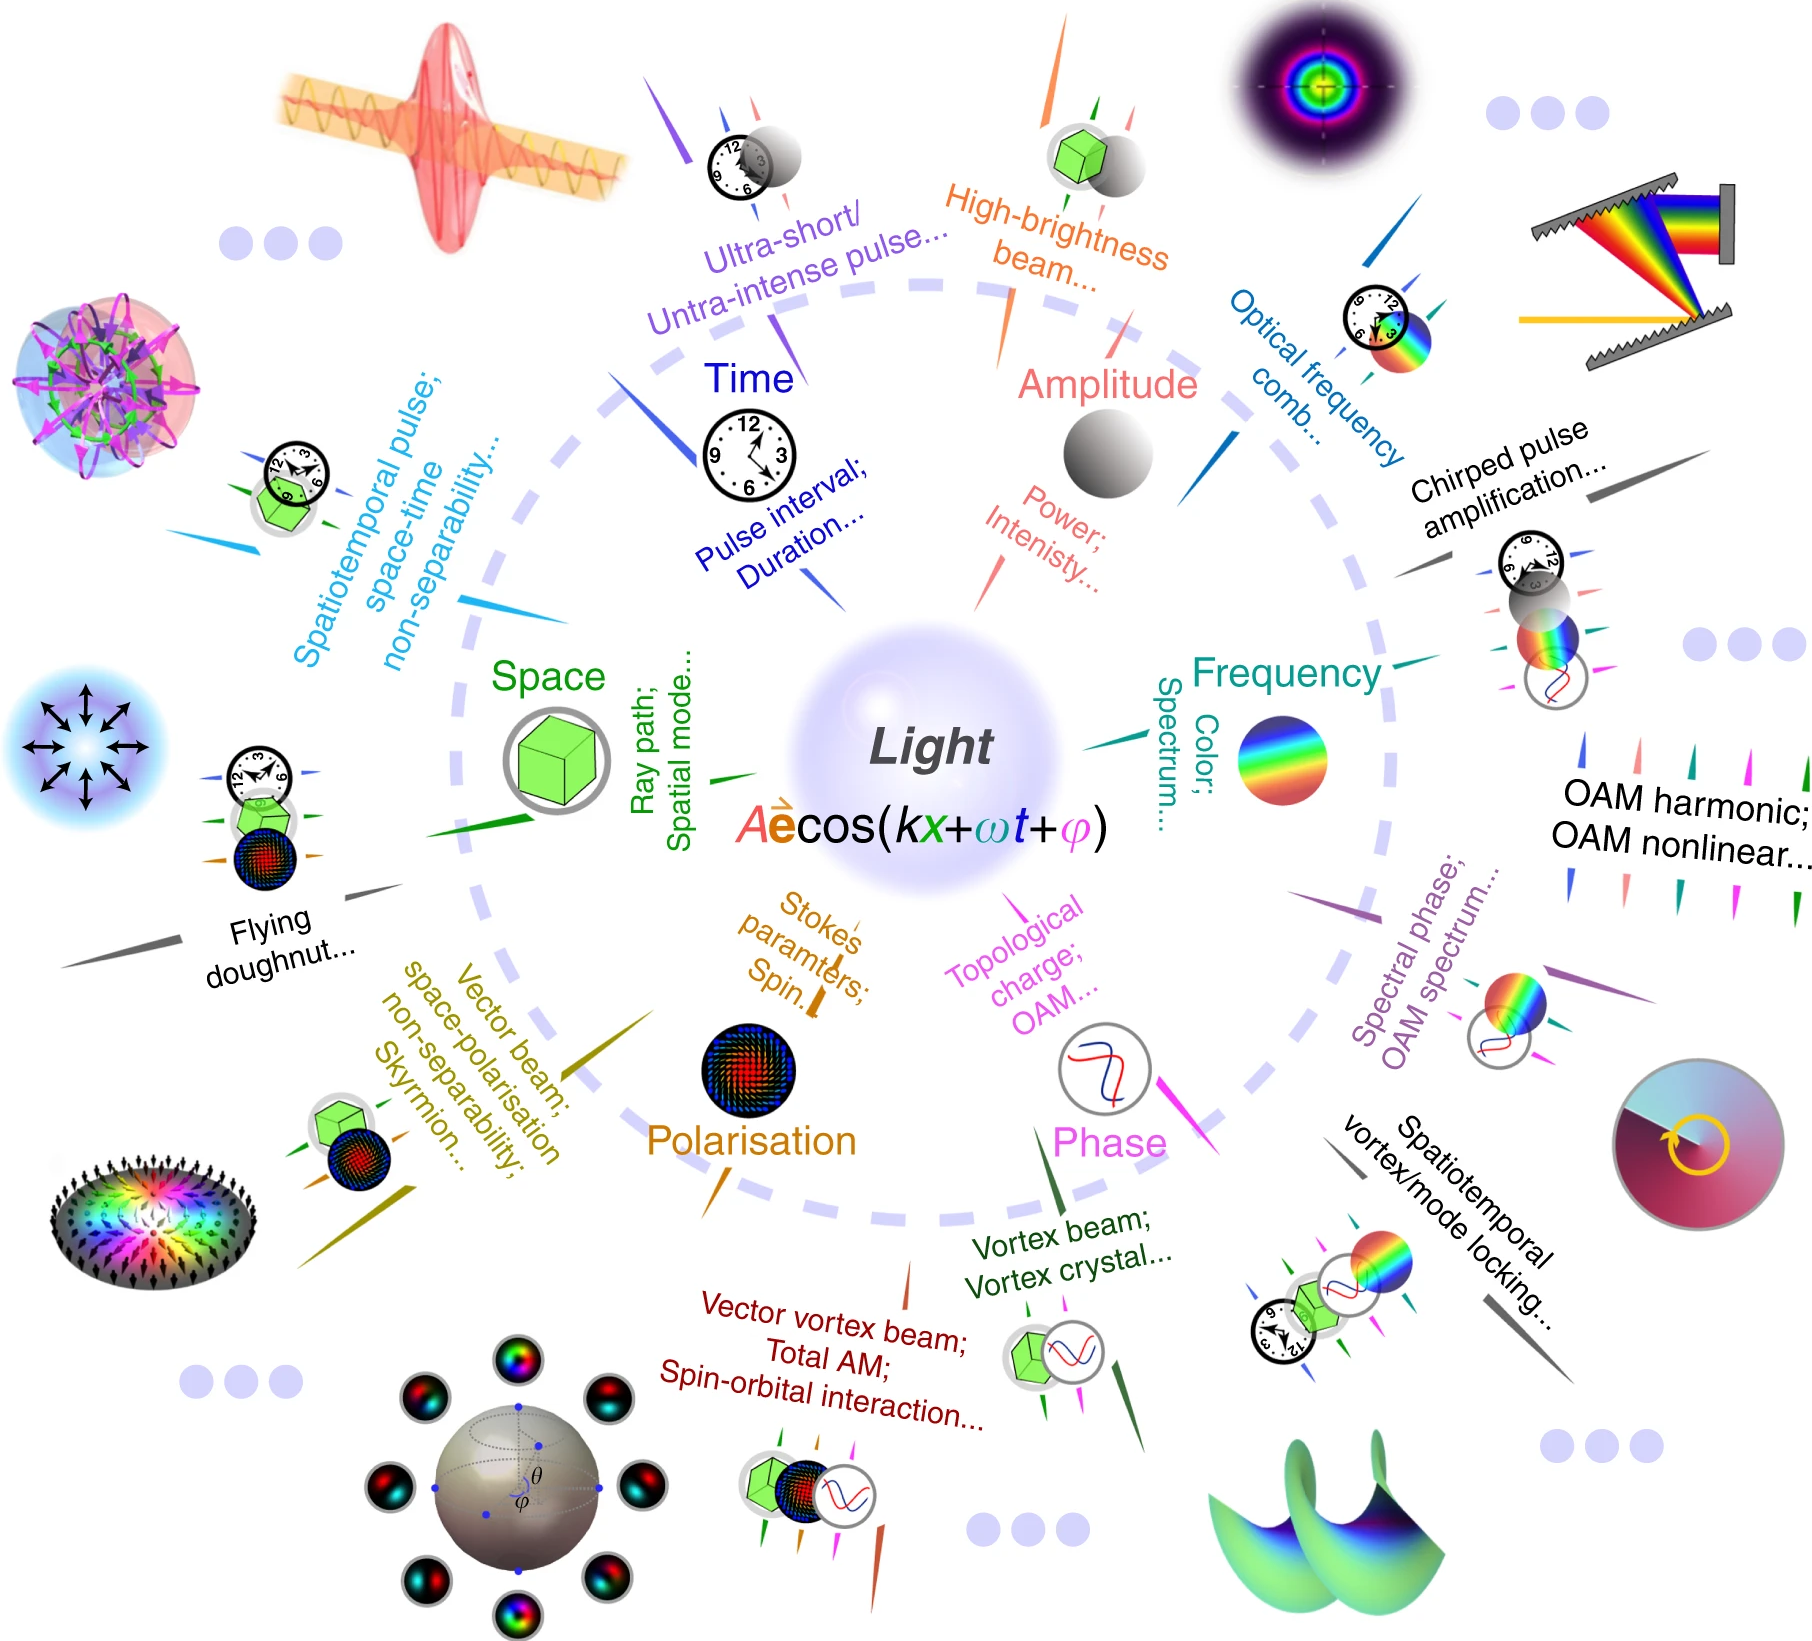
\includegraphics[width=1.0\textwidth,height=6.5cm,keepaspectratio]{img/towards_light.png}\\
	  {\tiny He et al., \textit{Nat.\ Rev.\ Phys.}\ \textbf{4}, 170 (2022) \cite{he2022towards}}
  \end{columns}
\end{frame}



% [I-2] LG Mode Fundamentals -- MOVED UP: this is the target basis, foundational
\begin{frame}{LG Mode Fundamentals}
  \centering
  \[
  u_{p,\ell}(r,\phi,z)=\sqrt{\frac{2p!}{\pi(p+|\ell|)!}}\,\frac{1}{w(z)}
  \left(\frac{\sqrt{2}r}{w(z)}\right)^{|\ell|}
  L_p^{|\ell|}\!\!\left(\frac{2r^2}{w^2(z)}\right)
  e^{-\frac{r^2}{w^2(z)}}\,
  e^{\frac{ikr^2}{2R(z)}}\,
  \textcolor{NYCUblue}{\bm{e^{i\ell\phi}}}\,
  e^{-i(2p+|\ell|+1)\psi(z)}
  \]
  {\small \textcolor{NYCUblue}{highlight term}: helical phase, carries topological charge $\ell$}
  \vspace{1pt}
  \begin{columns}[T]
    \column{0.40\textwidth}
      \begin{block}{Properties}
        \begin{itemize}
          \item $\ell$: topological charge; $L_z=\ell\hbar$
          \item Peak ring: $r_{\rm peak}=w_0\sqrt{|\ell|/2}$
        \end{itemize}
      \end{block}
      \vspace{1pt}
    \column{0.57\textwidth}
      \centering
      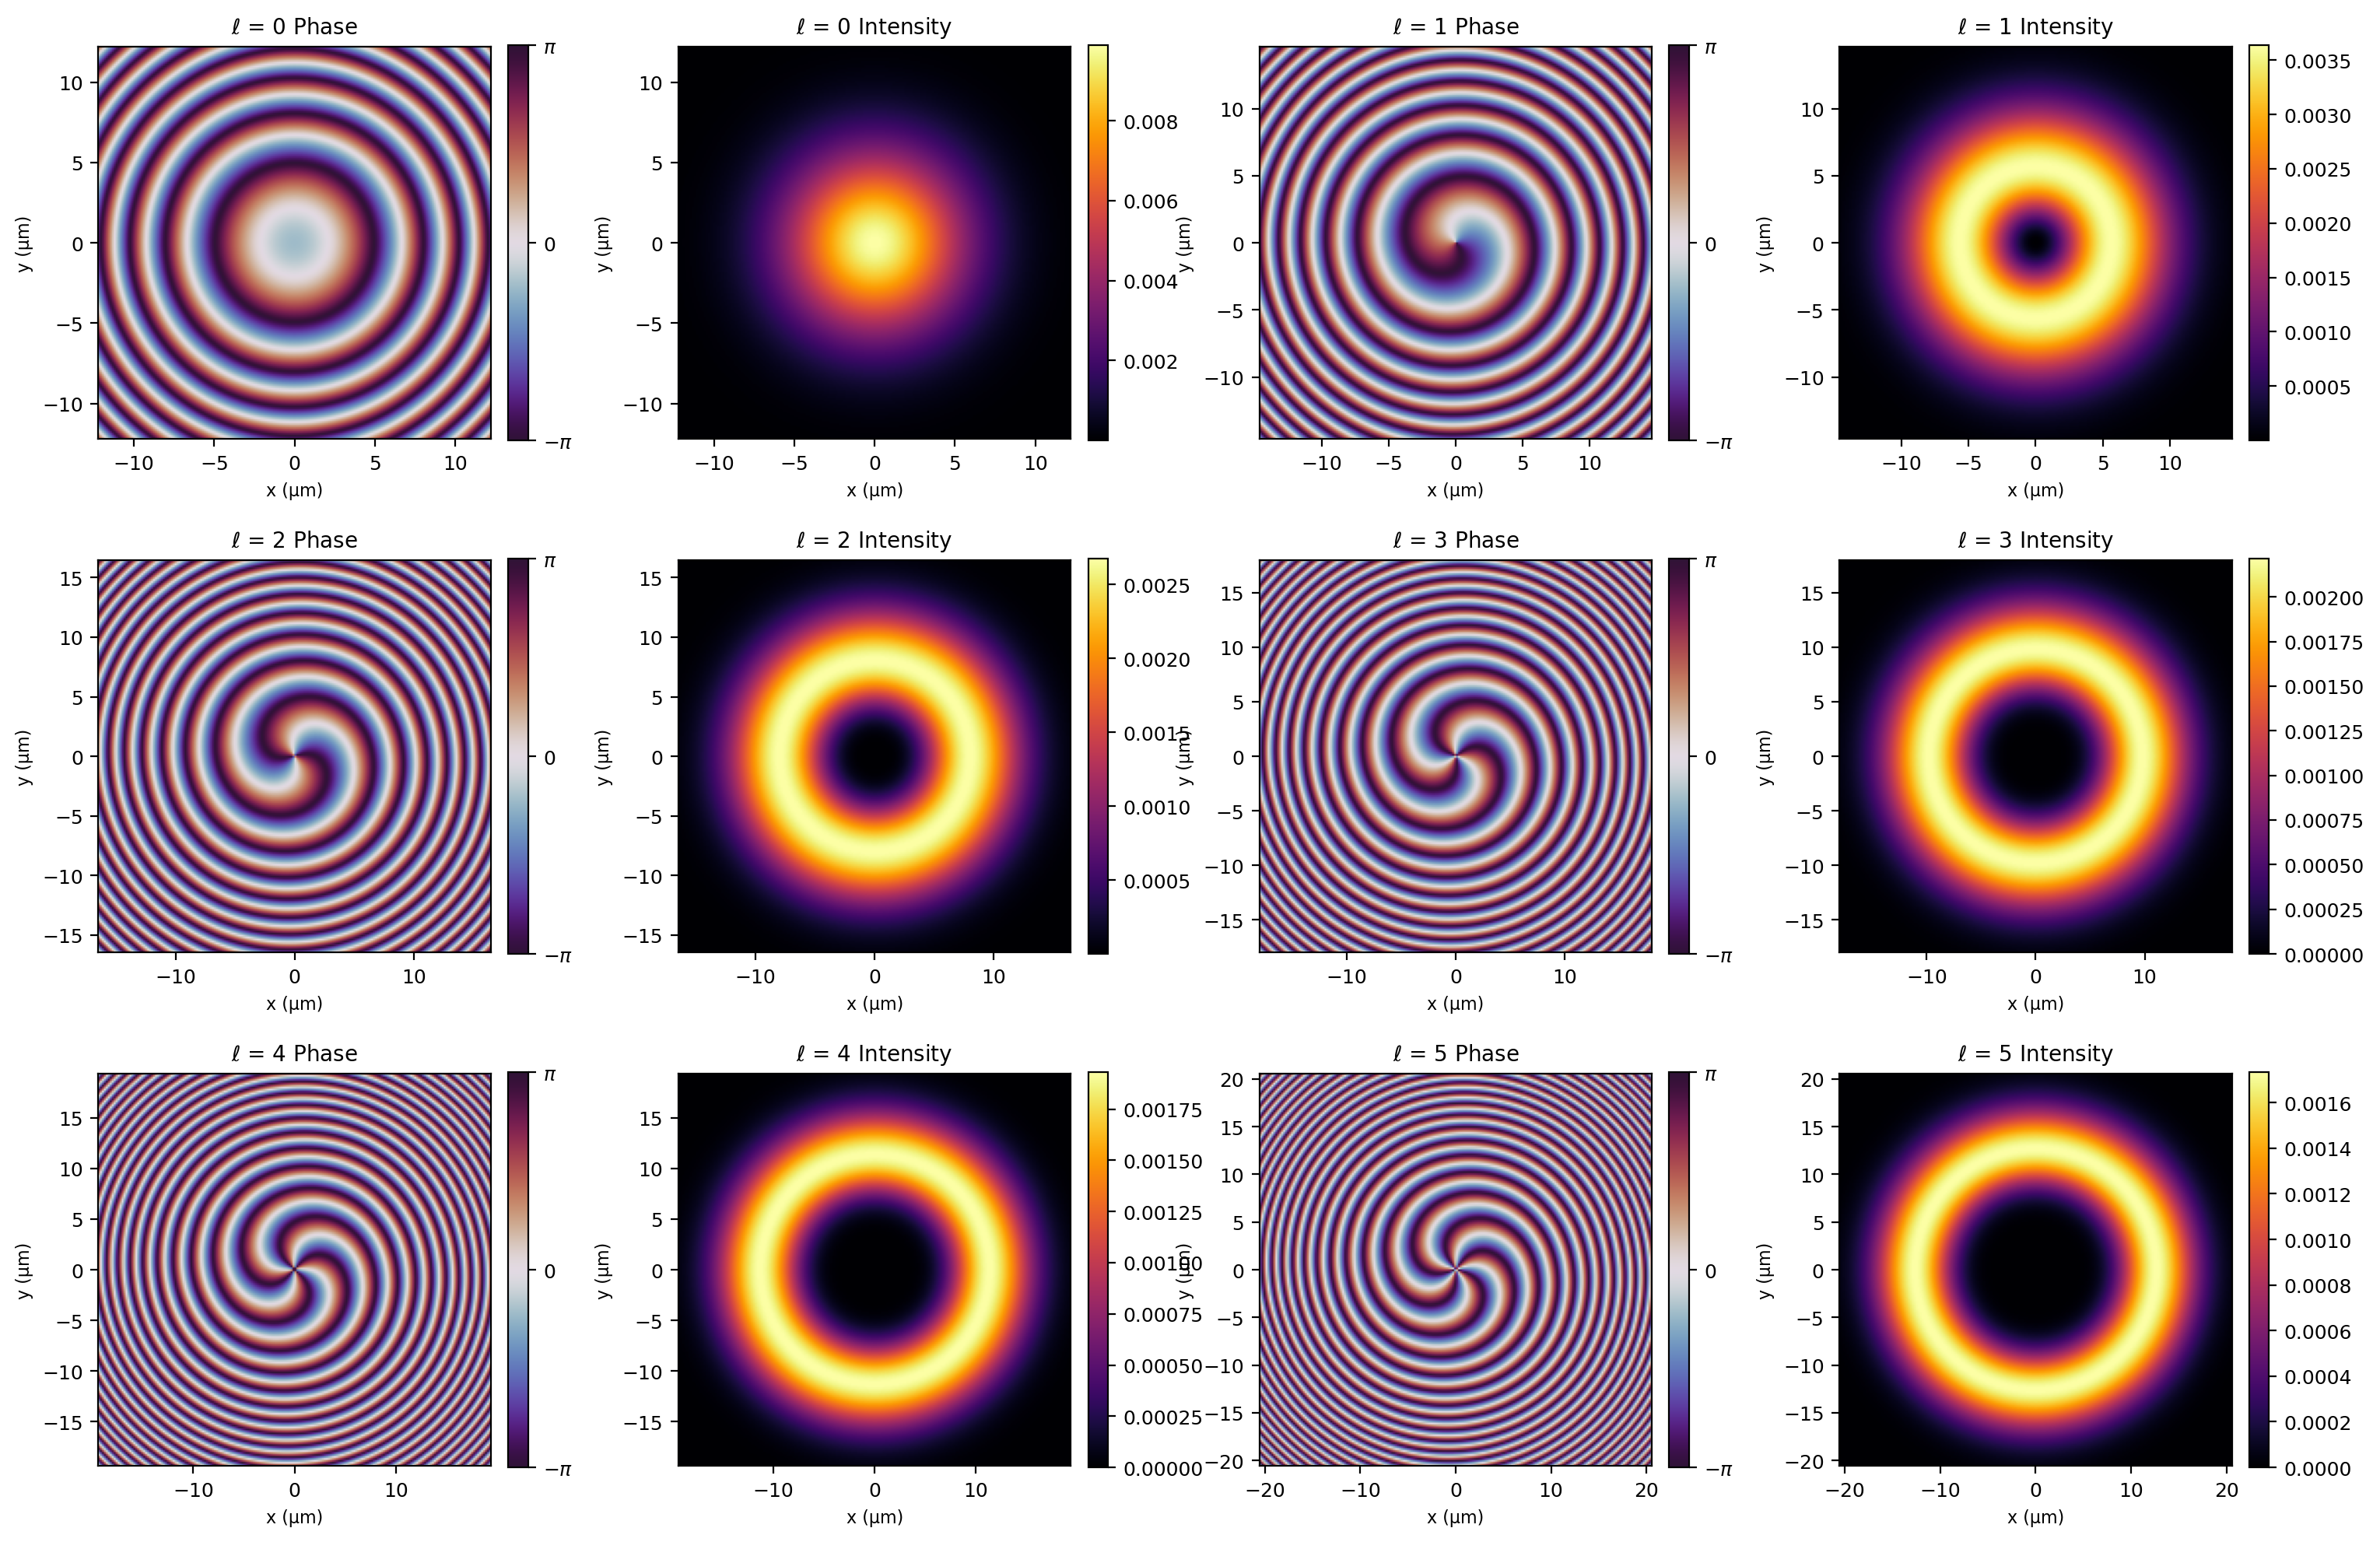
\includegraphics[width=1.0\textwidth,height=5.2cm,keepaspectratio]{img/target_LG_grid2x3.png}\\
  \end{columns}
\end{frame}


% VERIFY: D3h crystal-symmetry description flagged by student as needing
% verification against thesis main text -- unchanged here, verify before
% final print.


% [I-3] WS2 Valley Physics -- MOVED: narrows from "OAM in general" to
% "the specific active source this thesis uses". Empty itemize filled
% with 3 short bullets (images on the right already carry most of the
% visual information, per text-reduction instruction).

\begin{frame}{Transition Metal Dichalcogenides (TMDs)}
  
  \begin{columns}[T]
    \column{0.50\textwidth}
      \begin{block}{Properties of Monolayer $\text{WS}_2$, for example}
        \begin{itemize}
        \item Monolayer: indirect $\to$ \textbf{direct} bandgap
        \item Strong spin--orbit coupling
        \item broken inversion symmetry ($D_{3h}$)
        \item $K$/$K'$ valley selectivity
        \end{itemize}
      \end{block}
      \vspace{1pt}
      \begin{alertblock}{Valley Selection Rules}
        \centering
        \begin{tabular}{cc}
          \toprule
          Valley & Optical helicity \\
          \midrule
          $K$  & LCP ($\sigma^-$)  \\
          $K'$ & RCP ($\sigma^+$)  \\
          \bottomrule
        \end{tabular}
      \end{alertblock}
    \column{0.50\textwidth}
      \centering
      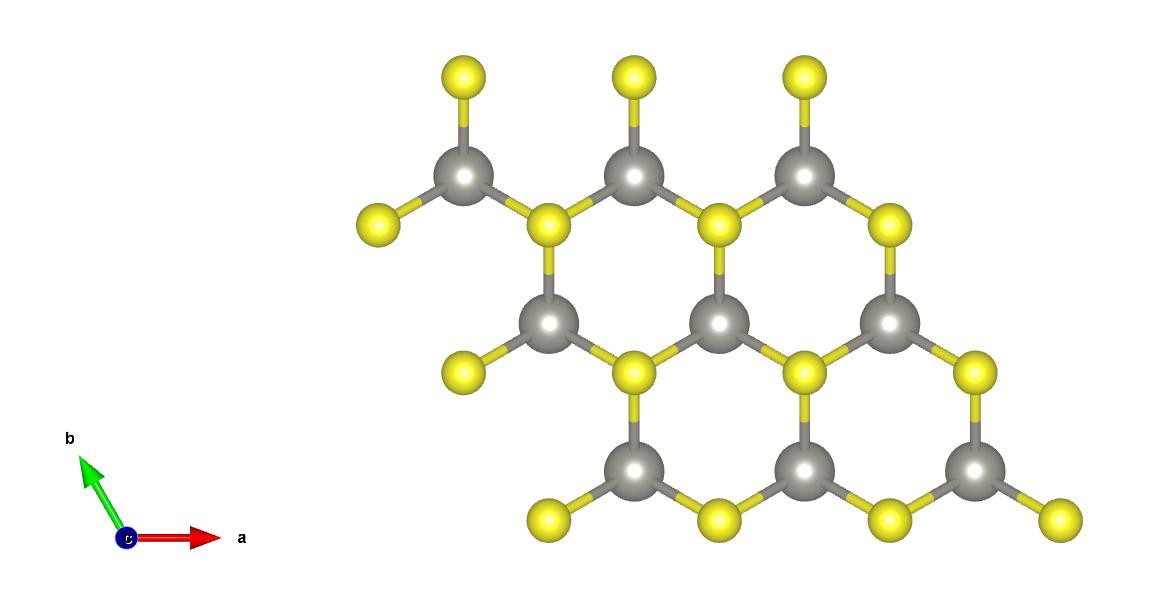
\includegraphics[width=0.85\textwidth,height=3.3cm,keepaspectratio]{img/TMDs_structure.jpg}\\[1pt]
      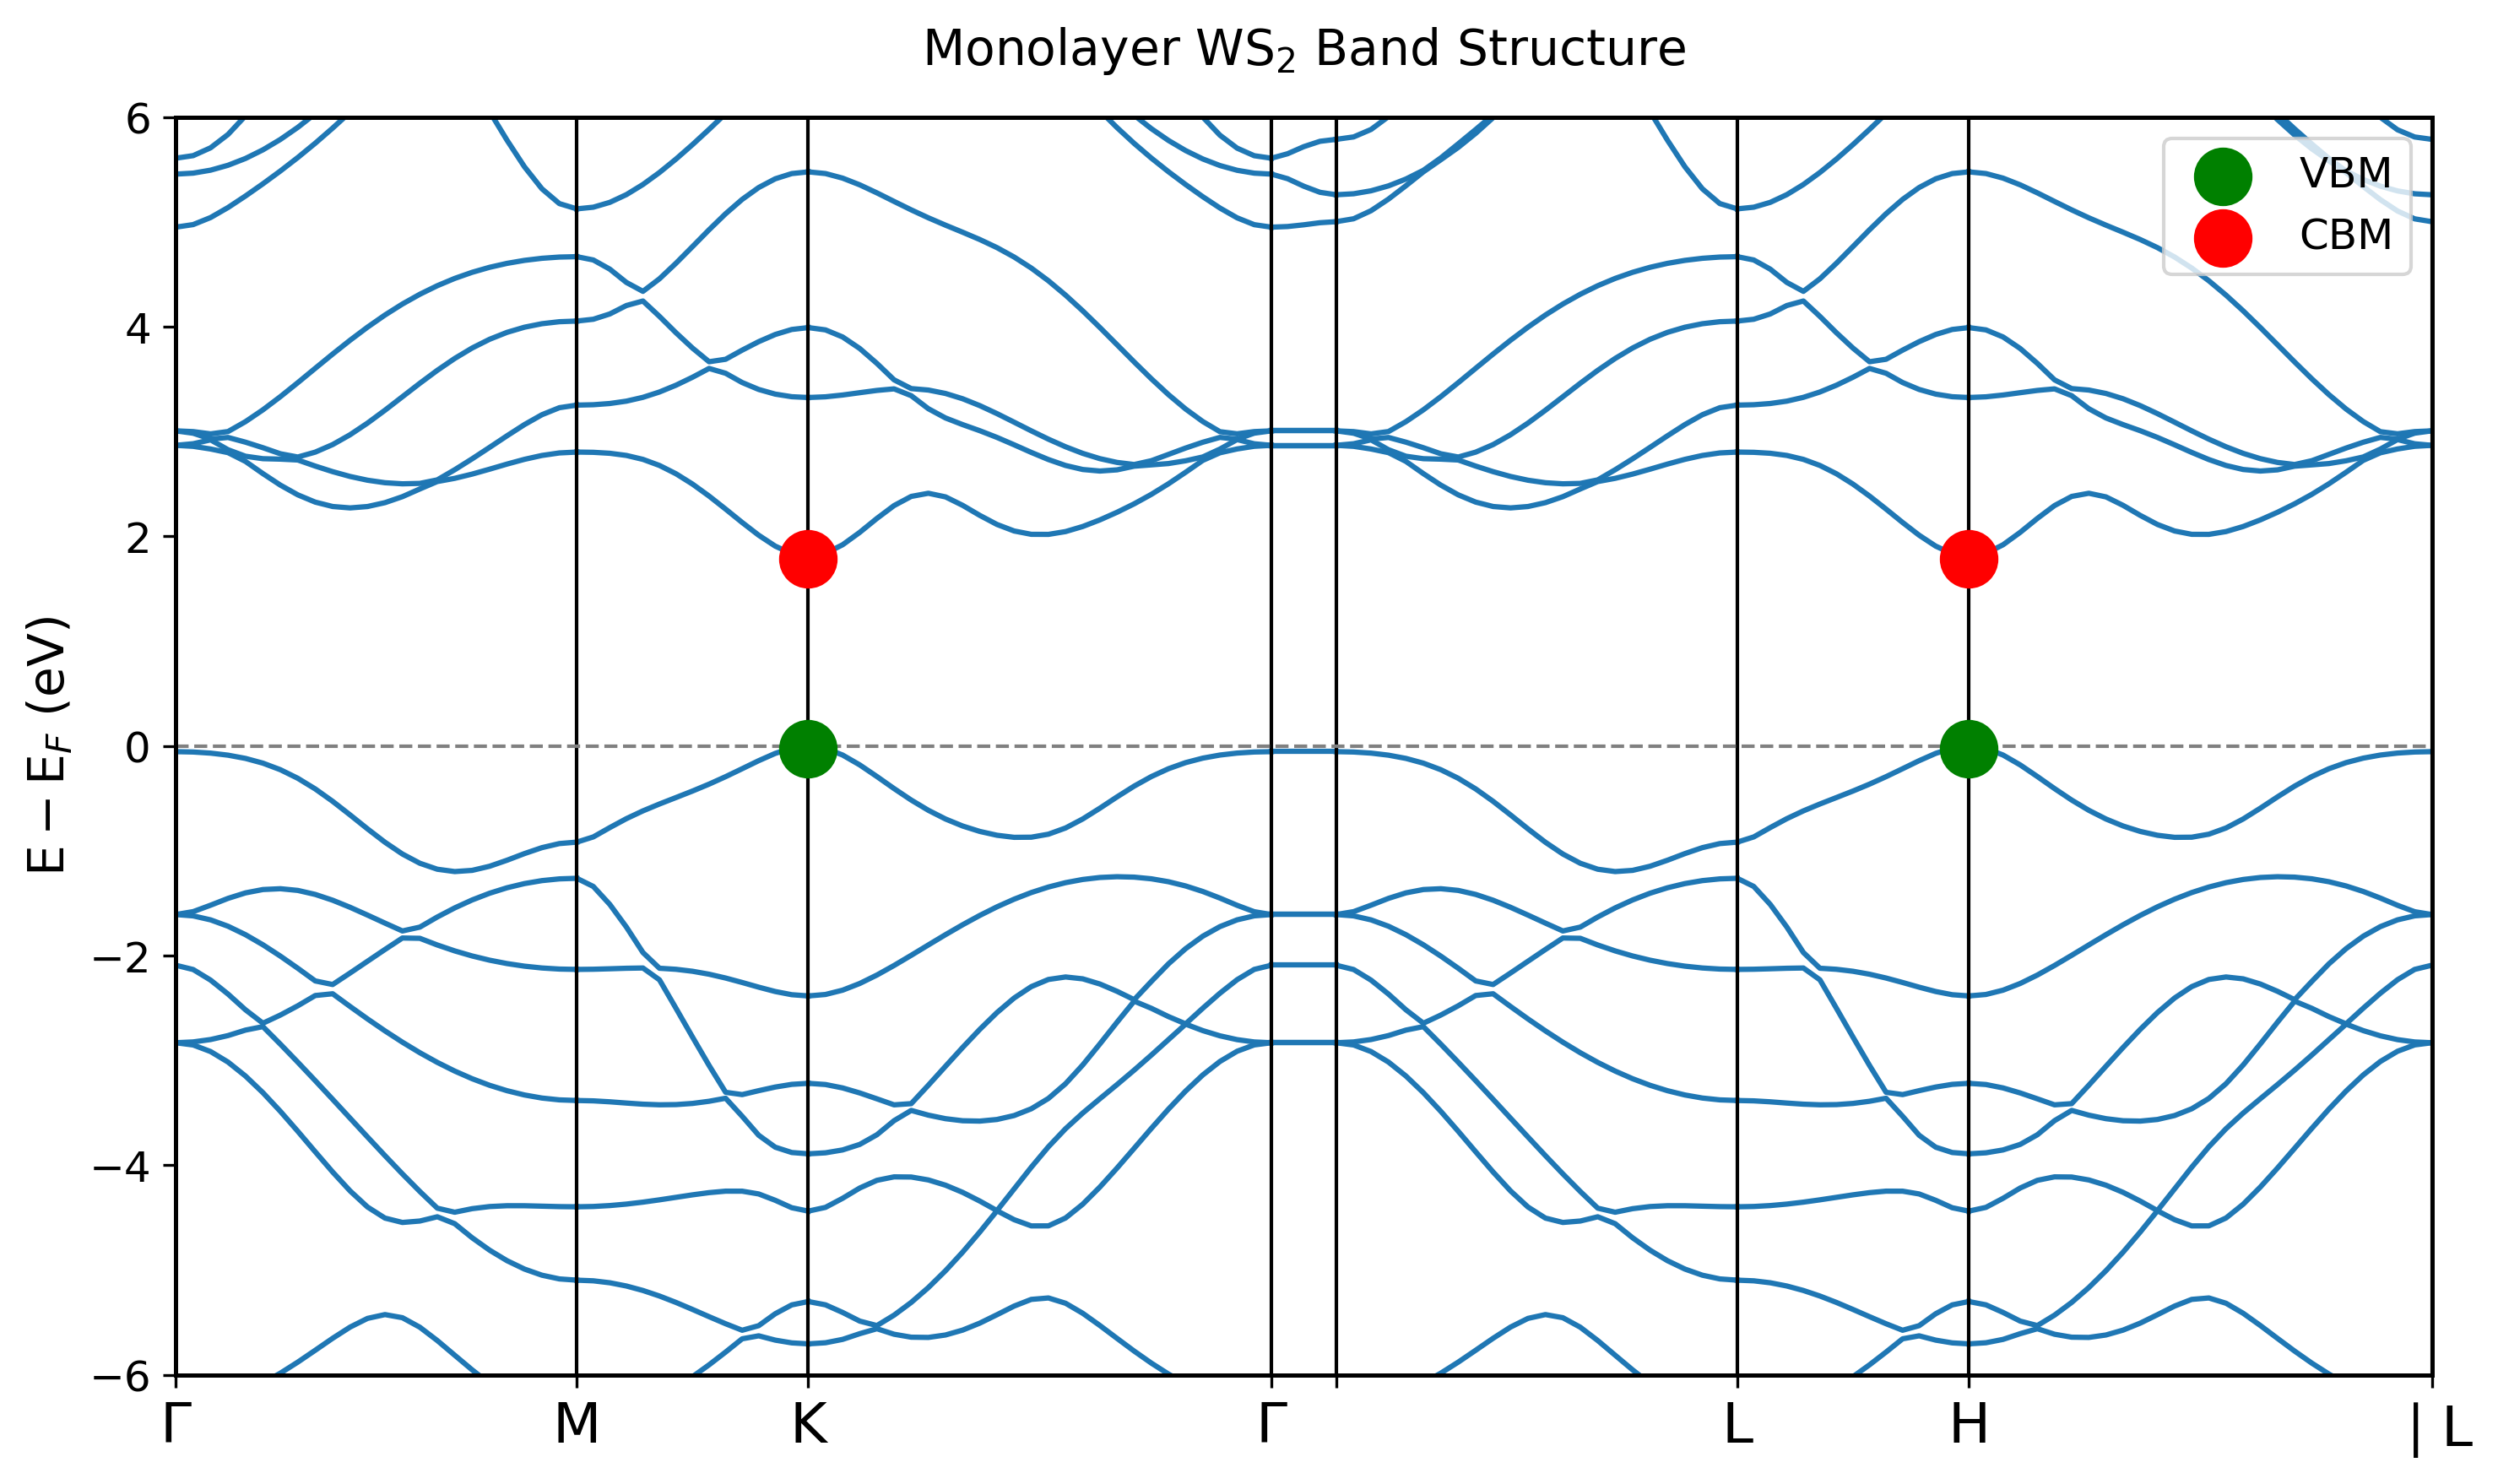
\includegraphics[width=0.85\textwidth,height=3.3cm,keepaspectratio]{img/WS2_8points_markers.png}
  \end{columns}
\end{frame}



% [I-5] Literature Timeline
% NOTE: Sroor 2020 is a committee member's work -- wording kept
% neutral/factual (no "outperform"-style language on this node).


\begin{frame}{Literature Timeline}
\centering

% ==================== 1. 上排 4 張圖片 ====================
\begin{columns}[T, totalwidth=\textwidth]
  \begin{column}{0.23\textwidth}
    \centering
    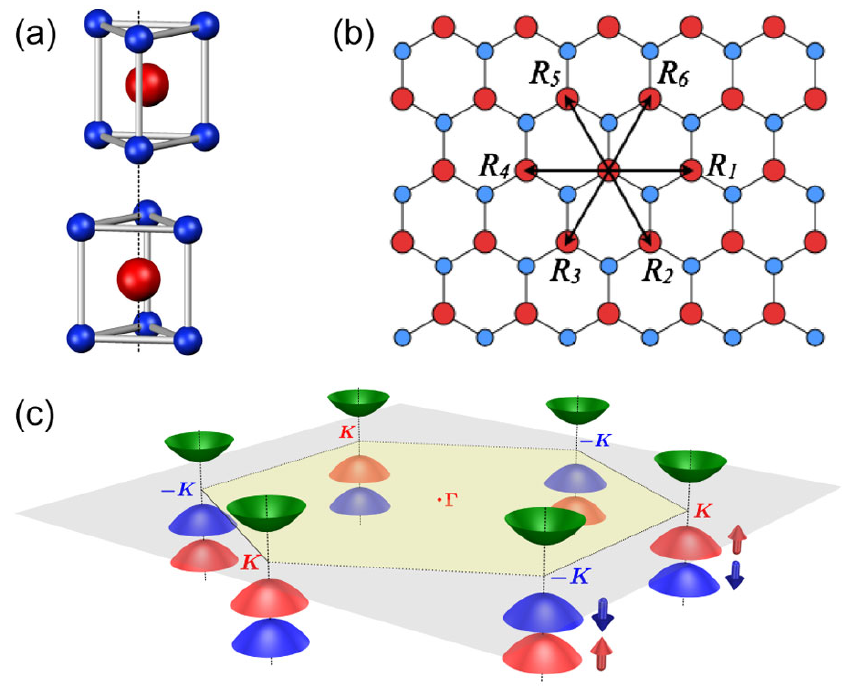
\includegraphics[width=\linewidth, height=2.2cm, keepaspectratio]{img/xiao2012.png}\\[1pt]
    {\tiny Xiao et al.~\cite{xiao2012coupled}}
  \end{column}
  \begin{column}{0.23\textwidth}
    \centering
    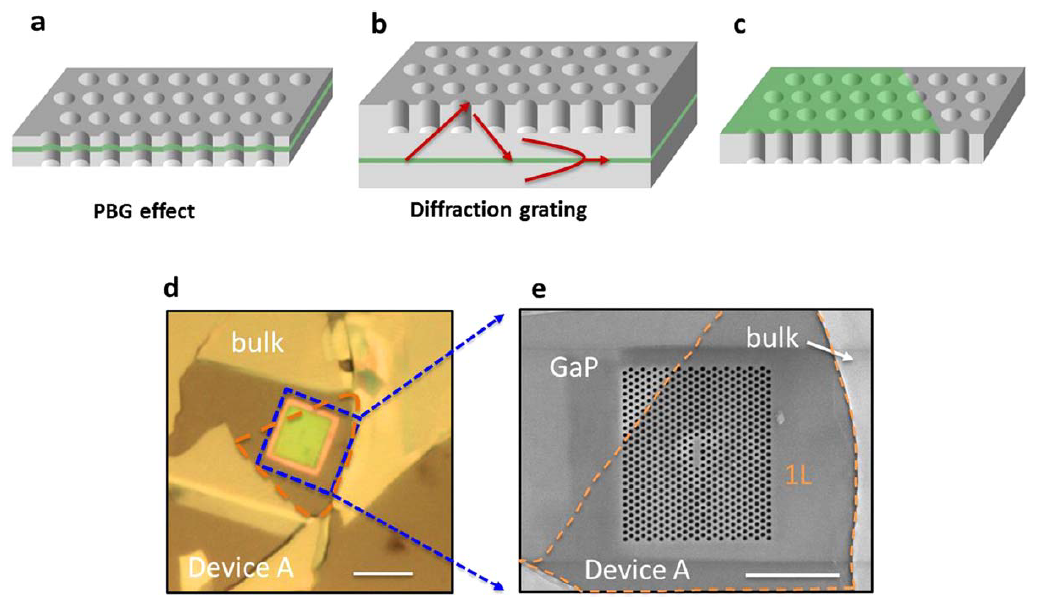
\includegraphics[width=\linewidth, height=2.2cm, keepaspectratio]{img/wu2014.png}\\[1pt]
    {\tiny Wu et al.~\cite{Wu2014control}}
  \end{column}
  \begin{column}{0.23\textwidth}
    \centering
    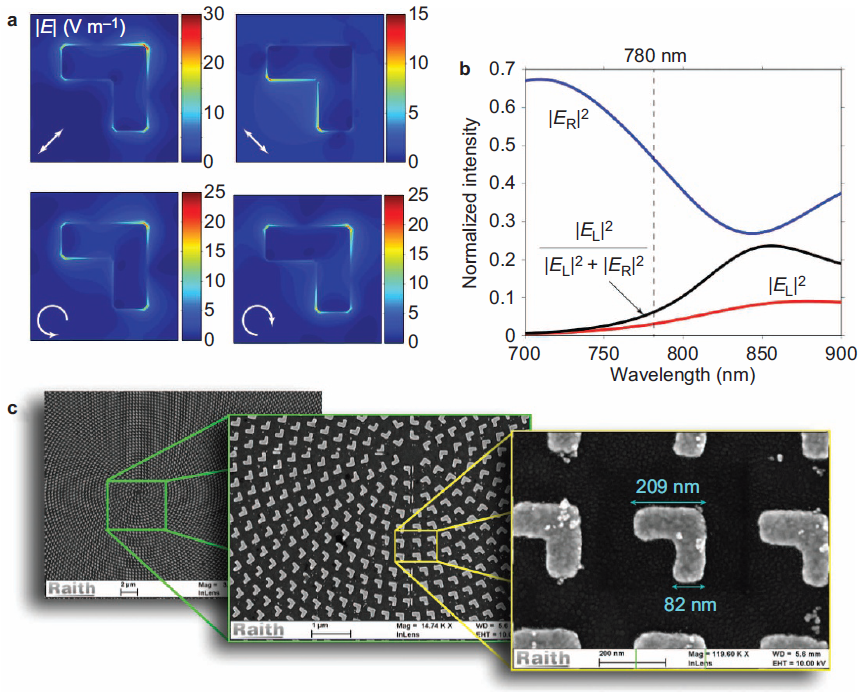
\includegraphics[width=\linewidth, height=2.2cm, keepaspectratio]{img/karimi2014.png}\\[1pt]
    {\tiny Karimi et al.~\cite{karimi2014generating}}
  \end{column}
  \begin{column}{0.23\textwidth}
    \centering
    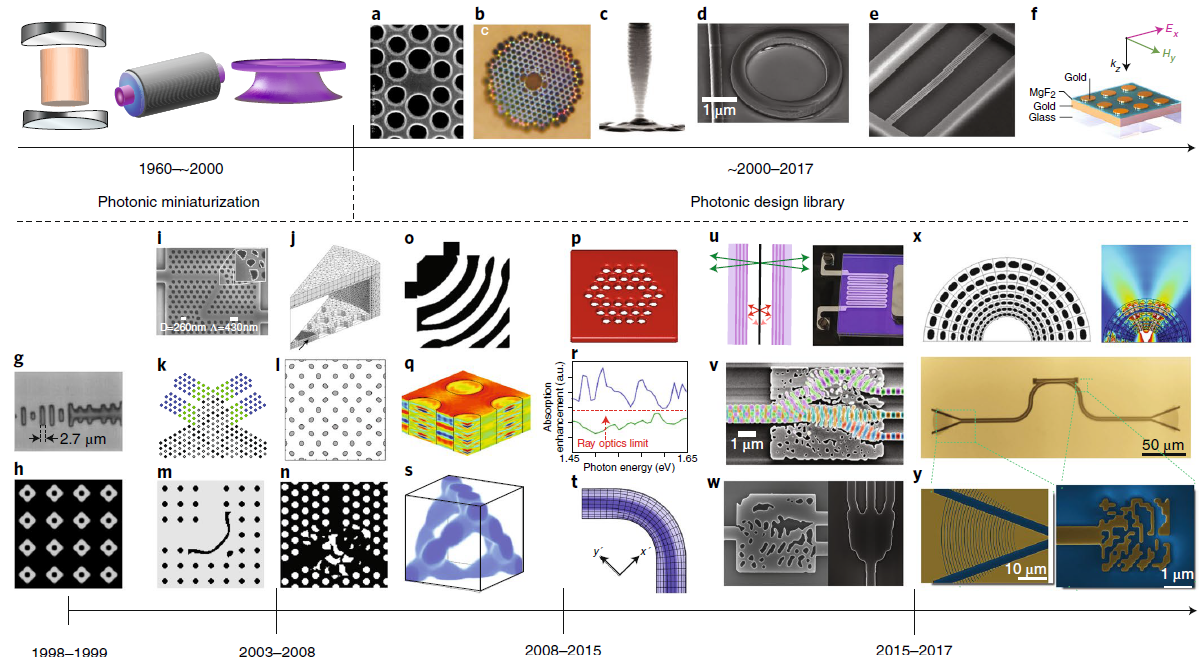
\includegraphics[width=\linewidth, height=2.2cm, keepaspectratio]{img/molesky2018.png}\\[1pt]
    {\tiny Molesky et al.~\cite{molesky2018inverse}}
  \end{column}
\end{columns}

\vspace{1pt}

% ==================== 2. 中間時間線與資訊 ====================
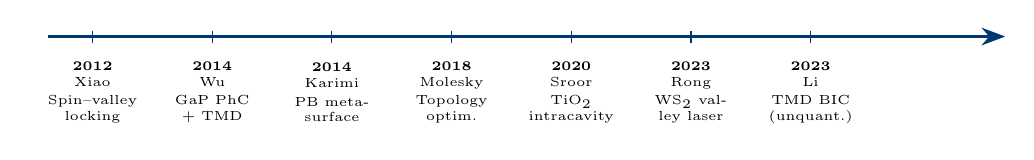
\begin{tikzpicture}[font=\tiny, scale=0.95, transform shape]
  % 時間軸橫線與箭頭
  \draw[thick, NYCUblue, -{Stealth[length=3mm]}] (-6.2,0) -- (6.6,0);

  % 刻度線
  \foreach \x in {-5.6,-4.0,-2.4,-0.8,0.8,2.4,4.0}{
    \draw[NYCUblue] (\x,0.08) -- (\x,-0.08);
  }

  % 2012 Xiao
  \node[align=center, text width=1.5cm] at (-5.6,-0.75)
    {\textbf{2012}\\Xiao\\[1pt]Spin--valley locking};

  % 2014 Wu
  \node[align=center, text width=1.5cm] at (-4.0,-0.75)
    {\textbf{2014}\\Wu\\[1pt]GaP PhC + TMD};

  % 2014 Karimi
  \node[align=center, text width=1.5cm] at (-2.4,-0.75)
    {\textbf{2014}\\Karimi\\[1pt]PB metasurface};

  % 2018 Molesky
  \node[align=center, text width=1.5cm] at (-0.8,-0.75)
    {\textbf{2018}\\Molesky\\[1pt]Topology optim.};

  % 2020 Sroor
  \node[align=center, text width=1.5cm] at (0.8,-0.75)
    {\textbf{2020}\\Sroor\\[1pt]TiO$_2$ intracavity};

  % 2023 Rong
  \node[align=center, text width=1.5cm] at (2.4,-0.75)
    {\textbf{2023}\\Rong\\[1pt]$\text{WS}_2$ valley laser};

  % 2023 Li
  \node[align=center, text width=1.5cm] at (4.0,-0.75)
    {\textbf{2023}\\Li\\[1pt]TMD BIC (unquant.)};

\end{tikzpicture}
\vspace{1pt}

% ==================== 3. 下排 3 張圖  ====================
\begin{columns}[T, totalwidth=\textwidth]
  \begin{column}{0.23\textwidth}
    \centering
    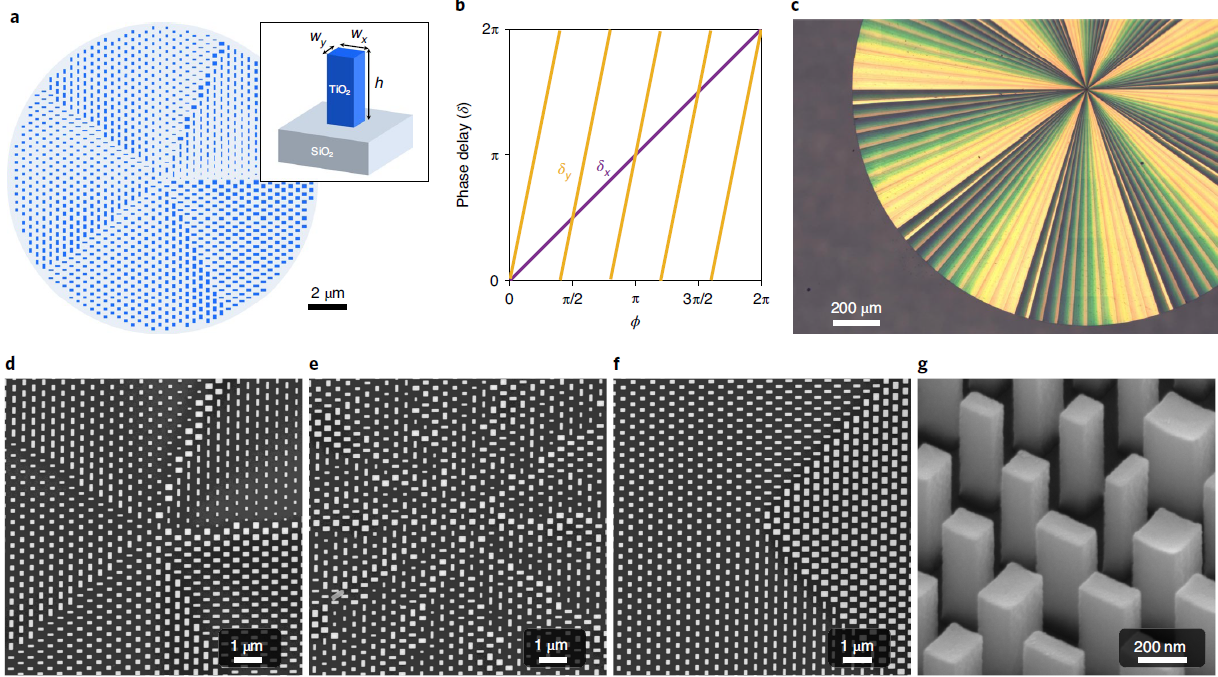
\includegraphics[width=\linewidth, height=2.2cm, keepaspectratio]{img/sroor2020.png}\\[1pt]
    {\tiny Sroor et al.~\cite{sroor2020high}}
  \end{column}
  \begin{column}{0.23\textwidth}
    \centering
    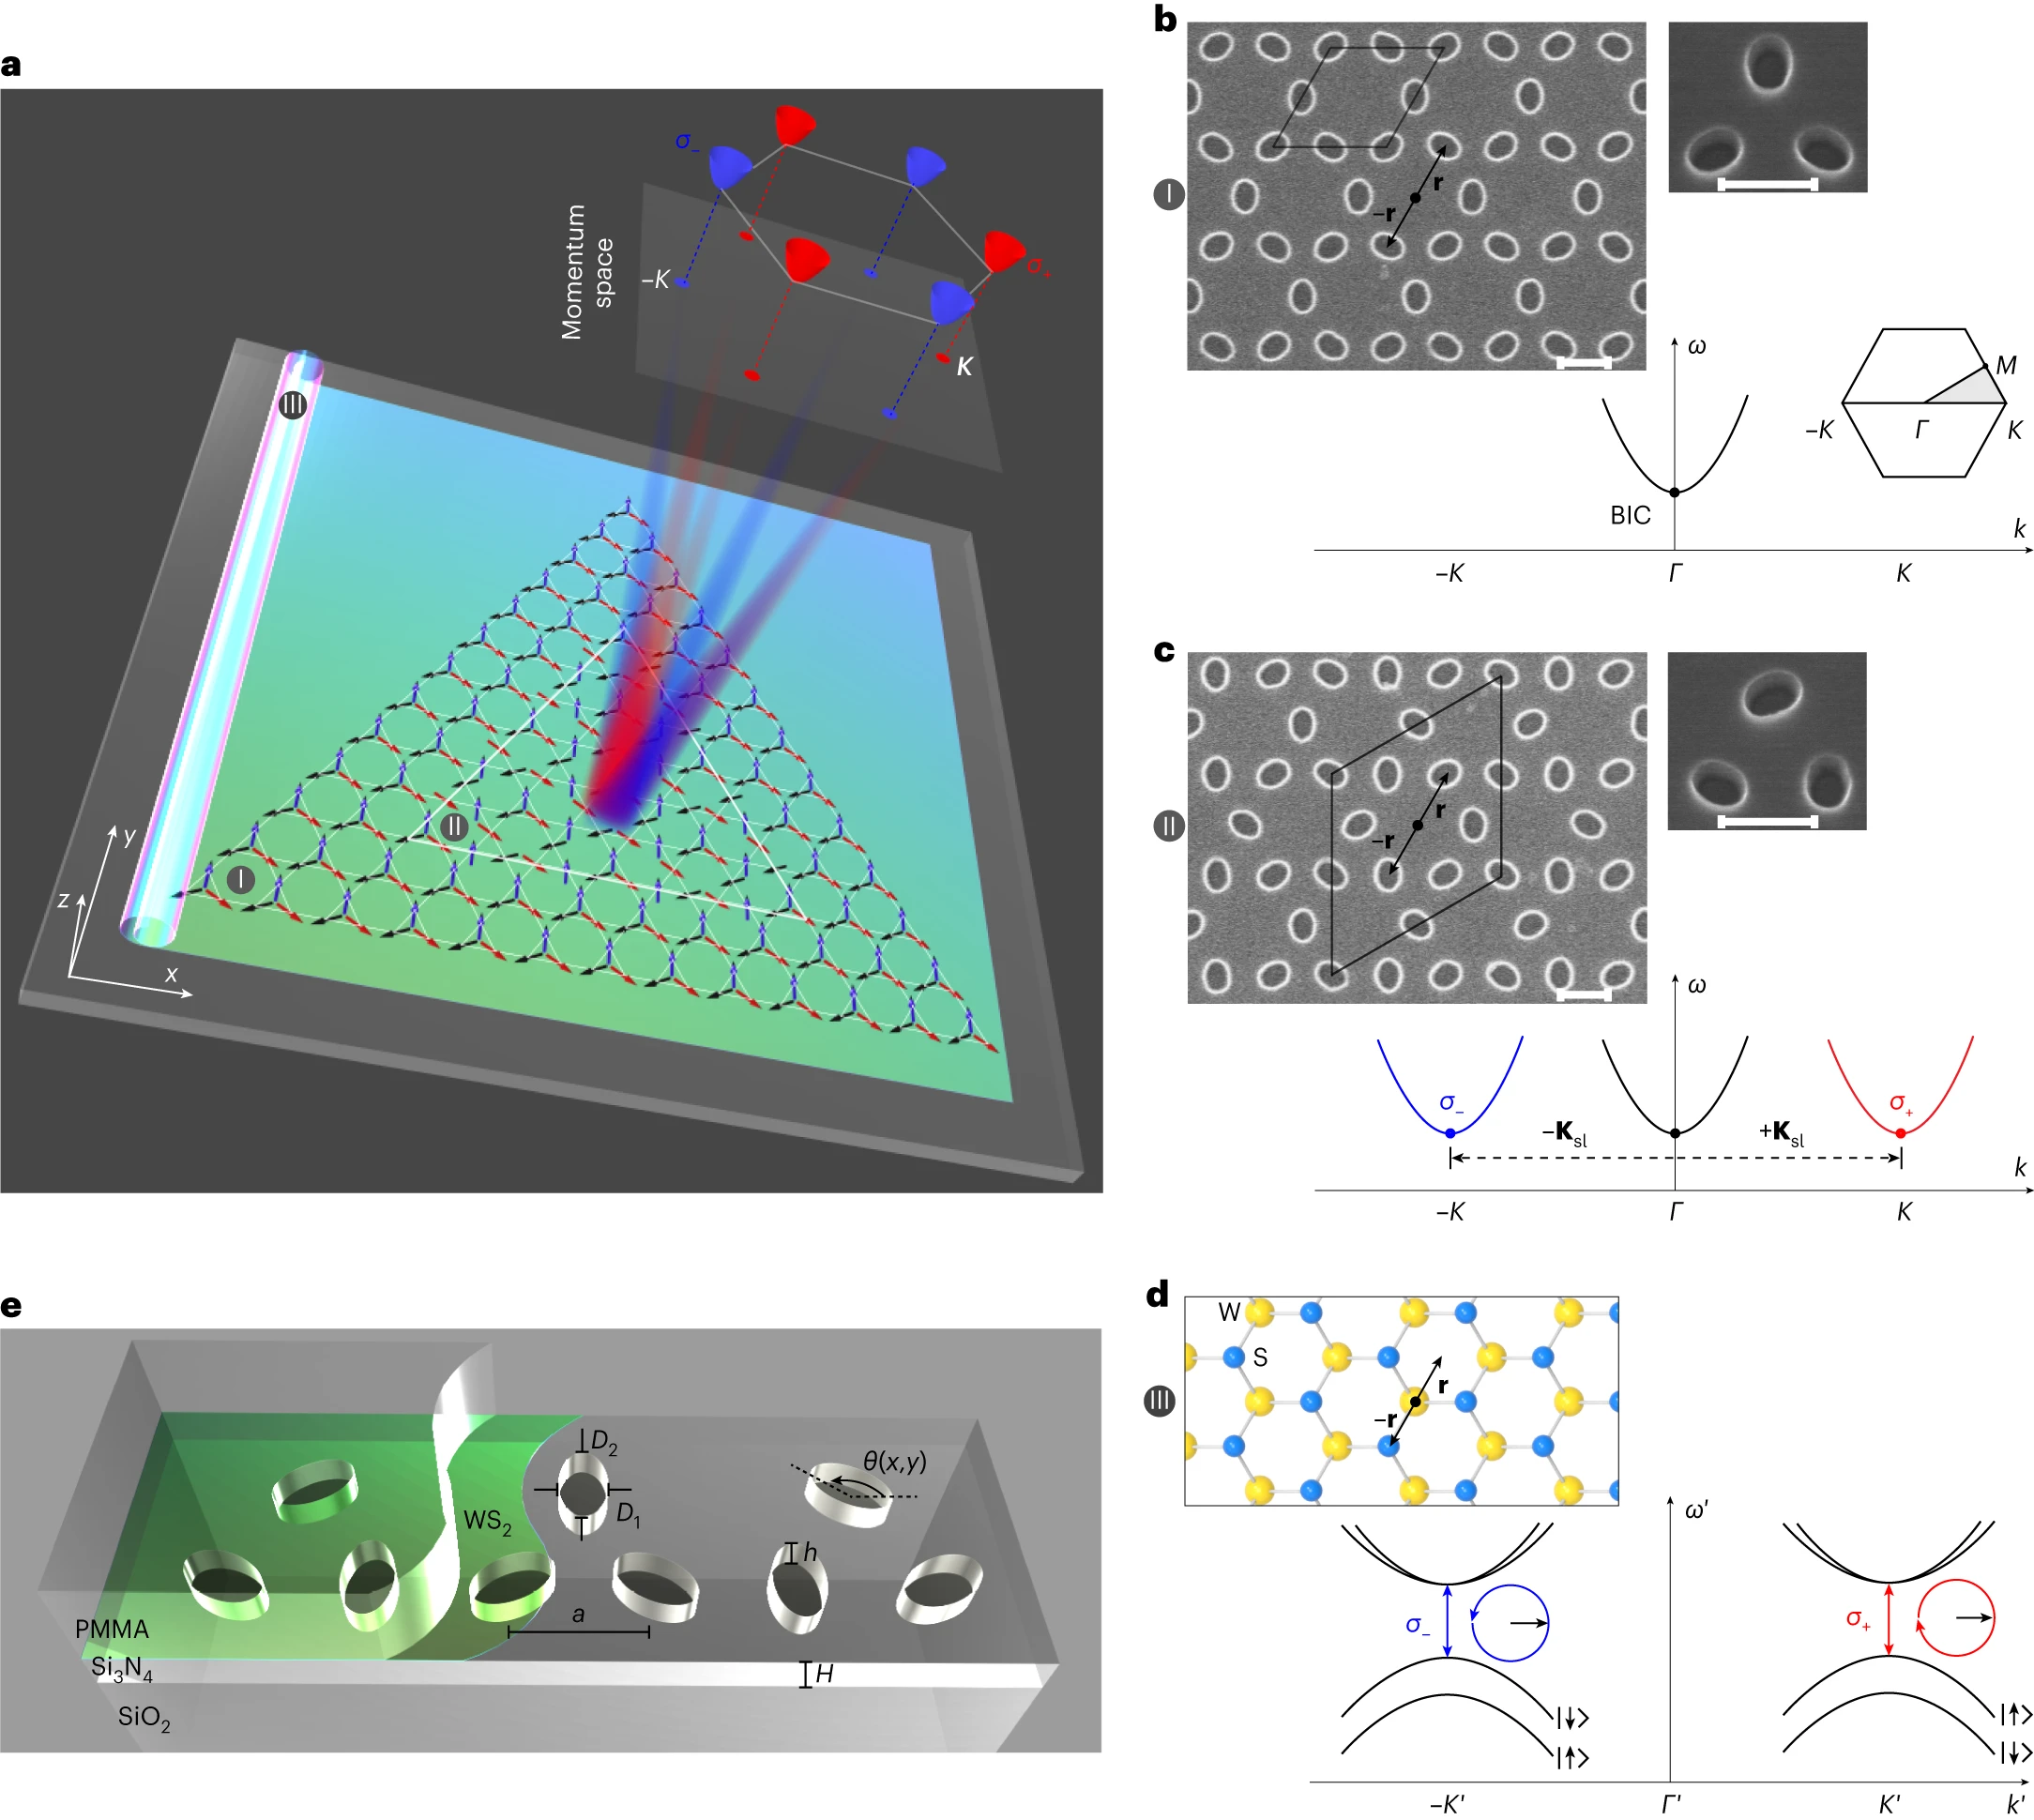
\includegraphics[width=\linewidth, height=2.2cm, keepaspectratio]{img/rong2023.png}\\[1pt]
    {\tiny Rong et al.~\cite{rong2023spin}}
  \end{column}
  \begin{column}{0.23\textwidth}
    \centering
    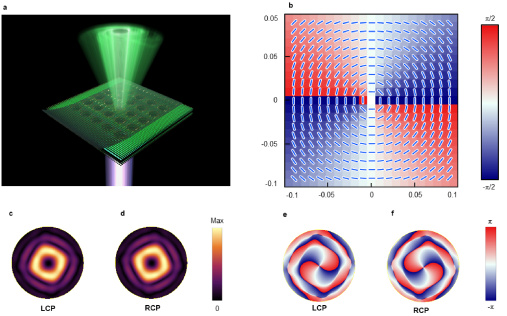
\includegraphics[width=\linewidth, height=2.2cm, keepaspectratio]{img/li2023.png}\\[1pt]
    {\tiny Li et al.~\cite{li2023valley}}
  \end{column}
\end{columns}
\vspace{1pt}
{\small \textbf{Gap:} no prior work combines active valley source \textbf{+} inverse design \textbf{+} quantified valley-OAM contrast.}
\end{frame}

% VERIFY: "Rong" appears here as 2023 / WS2 spin-valley laser, but the
% Backup literature table (Backup II) lists "2020 Rong -- Si metasurface,
% photonic Rashba" -- please confirm whether these are the same or two
% different Rong papers before the defense.


% [I-6] Motivation & Research Gap & Thesis Objectives -- narrowest point
% of the funnel: this specific thesis. Unchanged from v2.

\begin{frame}{Motivation, Research Gap \& Thesis Objectives}
  \begin{columns}[T]
    \column{0.40\textwidth}
      \centering
      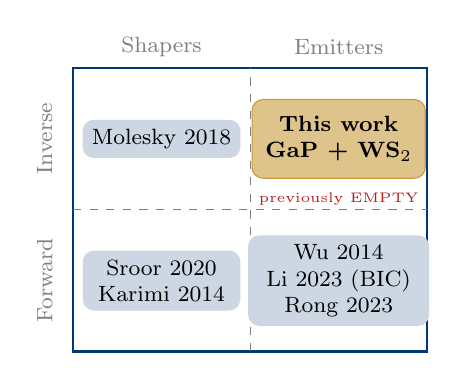
\begin{tikzpicture}[font=\small, scale=0.9]
        \draw[thick, NYCUblue] (0,0) rectangle (5,4);
        \draw[dashed, gray] (2.5,0) -- (2.5,4);
        \draw[dashed, gray] (0,2)   -- (5,2);
        \node[font=\footnotesize,gray] at (1.25,4.3) {Shapers};
        \node[font=\footnotesize,gray] at (3.75,4.3) {Emitters};
        \node[font=\footnotesize,gray,rotate=90] at (-0.4,1.0) {Forward};
        \node[font=\footnotesize,gray,rotate=90] at (-0.4,3.0) {Inverse};
        \node[fill=NYCUblue!20,rounded corners,align=center,font=\footnotesize,minimum width=2cm] at (1.25,1.0) {Sroor 2020\\Karimi 2014};
         \node[fill=NYCUblue!20,rounded corners,align=center,font=\footnotesize,minimum width=2.3cm] at (3.75,1.0) {Wu 2014\\Li 2023 (BIC)\\Rong 2023};
		\node[fill=NYCUblue!20,rounded corners,align=center,font=\footnotesize,minimum width=2cm] at (1.25,3.0) {Molesky 2018};
        \node[fill=NYCUgold!60,draw=NYCUgold,rounded corners,align=center,font=\footnotesize\bfseries,minimum width=2.2cm,minimum height=1.0cm] at (3.75,3.0) {\textbf{This work}\\GaP + $\text{WS}_2$};
        \node[accentred,font=\tiny] at (3.75,2.15) {previously EMPTY};
      \end{tikzpicture}
    \column{0.60\textwidth}
        \begin{alertblock}{Motivation}
        Chip-integrated, valley-controlled structured light emitter
      \end{alertblock}
      \begin{block}{Objectives}
        \begin{itemize}
          \item 3D FDTD + adjoint framework for $\text{WS}_2$ + GaP metasurface
          \item Inversely design valley-controlled LG emitters ($\ell=0$--$5$)
          \item Quantify: purity, phase winding, chirality propagation, inter-valley contrast
        \end{itemize}
      \end{block}
  \end{columns}
\end{frame}



\section{Methods}



% [DIVIDER-2]

\begin{frame}[plain]
  \begin{tikzpicture}[remember picture, overlay]
    \fill[NYCUblue](current page.south west) rectangle (current page.north east);
    \node[white,font=\Huge\bfseries] at (current page.center){2.\ Methods};
    \node[white,font=\large] at ([yshift=-1.2cm]current page.center){Physical Model $\cdot$ Topology Optimization $\cdot$ Figure of Merit $\cdot$ Performance Metrics};
  \end{tikzpicture}

\end{frame}

  

% [M-1] FDTD + MEEP. Empty blocks filled with short bullets; the
% right-hand figure caption already documents the simulation cross-
% section, so "Simulation Setup" only adds the numbers not visible there.

\begin{frame}{FDTD via MEEP \& Physical Model}

  \begin{columns}[T]
    \column{0.42\textwidth}
      \begin{exampleblock}{Simulation Setup}
        \begin{itemize}
        \item Resolution 50 pts/$\mu$m
        \item PML 0.3\,$\mu$m
        \item $\text{WS}_2$ $K$-valley LCP
        \item Near-field monitor $\to$ Far-field (10$z_R$)
        \item Design region $4.5\times4.5\times0.257\;\mu\text{m}^3$ \\
        \end{itemize}
      \end{exampleblock}
    \column{0.55\textwidth}
      \centering
      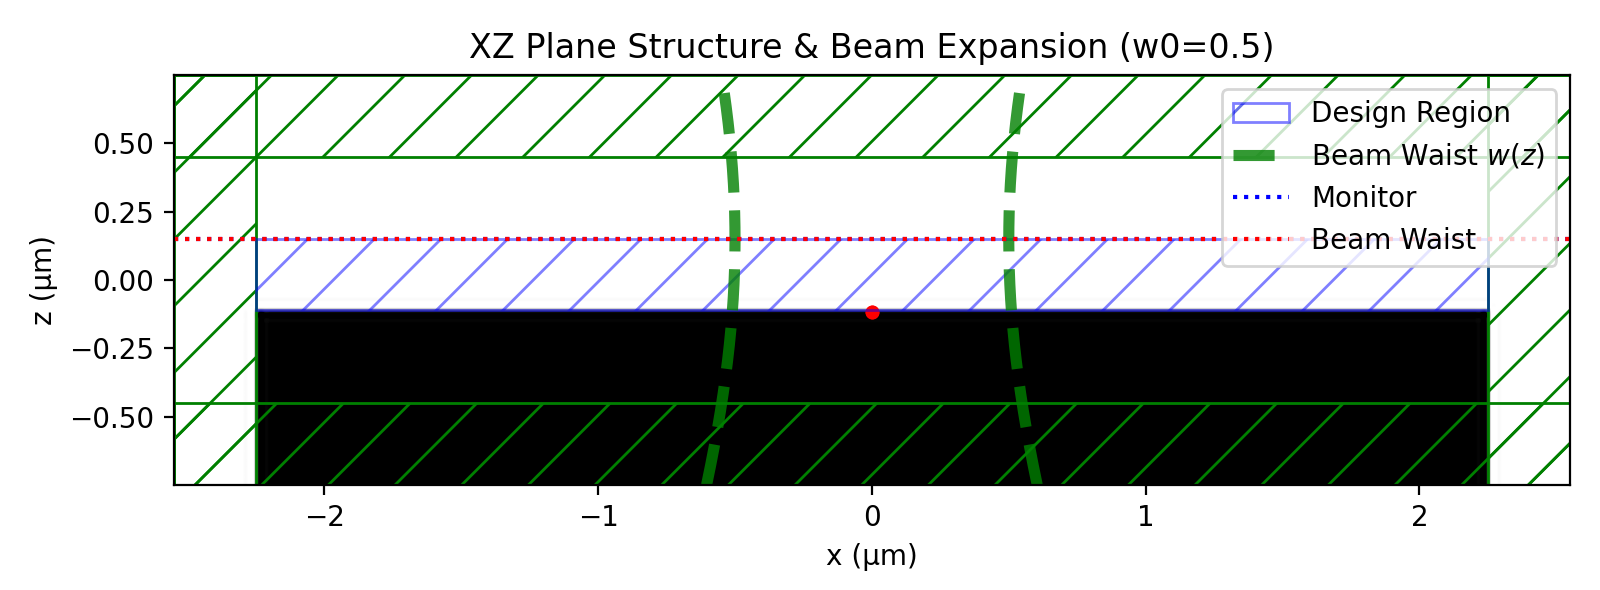
\includegraphics[width=\textwidth,keepaspectratio]{img/xz_structure_waist.png}\\
      {\tiny Cross-section: PML / Diamond / $\text{WS}_2$ dipole / GaP--Air design layer / NF monitor (red dashed) / Air / PML.}
  \end{columns}
\end{frame}


% [M-3] Topology Optimization I: Parametrization + N2F workflow.
% (Consolidated from the old, near-duplicate S13/S14/S15 -- see v3 log.)

\begin{frame}{Topology Optimization}
  \begin{columns}[T]
    \column{1.0\textwidth}
      \centering
      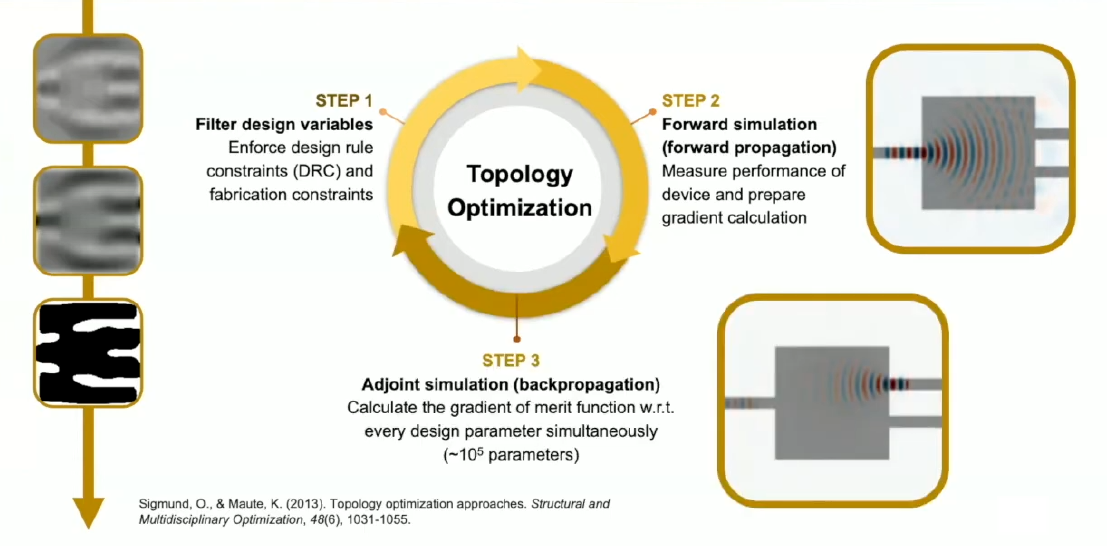
\includegraphics[width=0.8\textwidth,height=5.0cm,keepaspectratio]{img/to_workflow.png}\\
      {\tiny \cite{meepcon2022topology} Init $\to$ Forward FDTD $\to$ N2F $\to$ FOM $\to$ Adjoint FDTD $\to$ Gradient $\to$ MMA update. $\beta$ increases until $\beta_{\rm max}=512$.}
      \begin{minipage}{0.4\textwidth}
      \begin{block}{Tanh Projection}
      \centering
        $\bar{\rho}=\dfrac{\tanh(\beta\eta)+\tanh(\beta(\tilde{\rho}-\eta))}{\tanh(\beta\eta)+\tanh(\beta(1-\eta))}$
      \end{block}
      \end{minipage}
  \end{columns}
\end{frame}


% [M-5] Metrics -- unchanged from v2 (FOM back-reference now resolves to
% an actual definition on M-4 above).

\begin{frame}{Figure of Merit (FOM)}

{\footnotesize \[ P_\text{sim}=\int_A\!\left(E_{sim,x}E_{sim,x}^*+E_{sim,y}E_{sim,y}^*\right)dA \]}\\
{\footnotesize \[ P_\text{target}=\int_A\!\left(E_{t,x}E_{t,x}^*+E_{t,y}E_{t,y}^*\right)dA  \quad P_\text{target}=1\] }\\
{\footnotesize \[ \text{Overlap}=\int_A\!\left(E_{ff,x}E_{t,x}^*+E_{ff,y}E_{t,y}^*\right)dA \]}\\


  \begin{columns}[T]
    \column{0.48\textwidth}
      \begin{block}{FoM I}
        {\footnotesize \[ \text{FOM} = \dfrac{|\text{Overlap}|^{2}}{P_\text{sim} P_\text{target}} \]}
      \end{block}
    \column{0.48\textwidth}
      \begin{block}{FoM II}
        {\footnotesize \[ \text{FOM} = \log \dfrac{|\text{Overlap}|^{2}}{P_\text{sim} P_\text{target}} +\alpha \log|\text{Overlap}|^2 \quad\alpha=0.1 \]}
      \end{block}
  \end{columns}
\end{frame}


\begin{frame}{Performance Metrics}

  \begin{columns}[T]
    \column{0.48\textwidth}
      \begin{block}{\textcircled{1} Mode Overlap Integral}
        $|\text{Overlap}|^2$$\Rightarrow$ \text{absolute coupling power} {\scriptsize\textcolor{accentgreen}{($\uparrow$ better)}}
      \end{block}
      \vspace{1pt}
      \begin{block}{\textcircled{2} LG Mode Purity}
        \[ \text{Purity}=\frac{|\text{Overlap}|^2}{P_\text{sim} \cdot P_\text{target}}\]
        \textbf{Normalized shape fidelity}; $\in[0,1]$ {\scriptsize\textcolor{accentgreen}{($\uparrow$ better)}}
      \end{block}
    \column{0.48\textwidth}
      \begin{block}{\textcircled{3} Phase Winding}
        Unwrapped $\Delta\phi$ should $=\ell\times2\pi$\\
      \end{block}
      \vspace{1pt}
      \begin{block}{\textcircled{4} Optical Chirality}
        $C=\pi f\,\mathrm{Im}(\mathbf{E}^*\cdot\mathbf{H})$\\
        $C<0$: LCP;\quad $C>0$: RCP dominant\\
        Evaluated at near-field and $z=10\,z_R$
      \end{block}
    \vspace{2pt}
  \end{columns}
\end{frame}



\section{Results \& Discussion}



% [DIVIDER-3]

\begin{frame}[plain]
\begin{tikzpicture}[remember picture, overlay]
\fill[NYCUblue](current page.south west) rectangle (current page.north east);
\node[white,font=\Huge\bfseries] at (current page.center){3.\ Results \& Discussion};
\node[white,font=\large,align=center] at ([yshift=-1.2cm]current page.center){%
  FoMs $\cdot$ Structures $\cdot$ Far-Field $\cdot$ Phase winding \\%
  Chirality Propagation $\cdot$ Valley Selectivity $\cdot$ Device Energy Efficiency $\cdot$ Comparison%
};
\end{tikzpicture}
\end{frame}

% Results & Discussion frames below are UNCHANGED from v2 per your
% instruction -- this section keeps its full detail, no text reduction.

\begin{frame}{Compare FoMs}
  \begin{center}
    {\small $\ell=5$ , for example}\\[2pt]
    \begin{tabular}{cc}
    {\small Purity = 72.89\%, $|\text{Overlap}|^2$ = 0.89} & {\small Purity = 82.62\%, $|\text{Overlap}|^2$ = 3.96}\\
    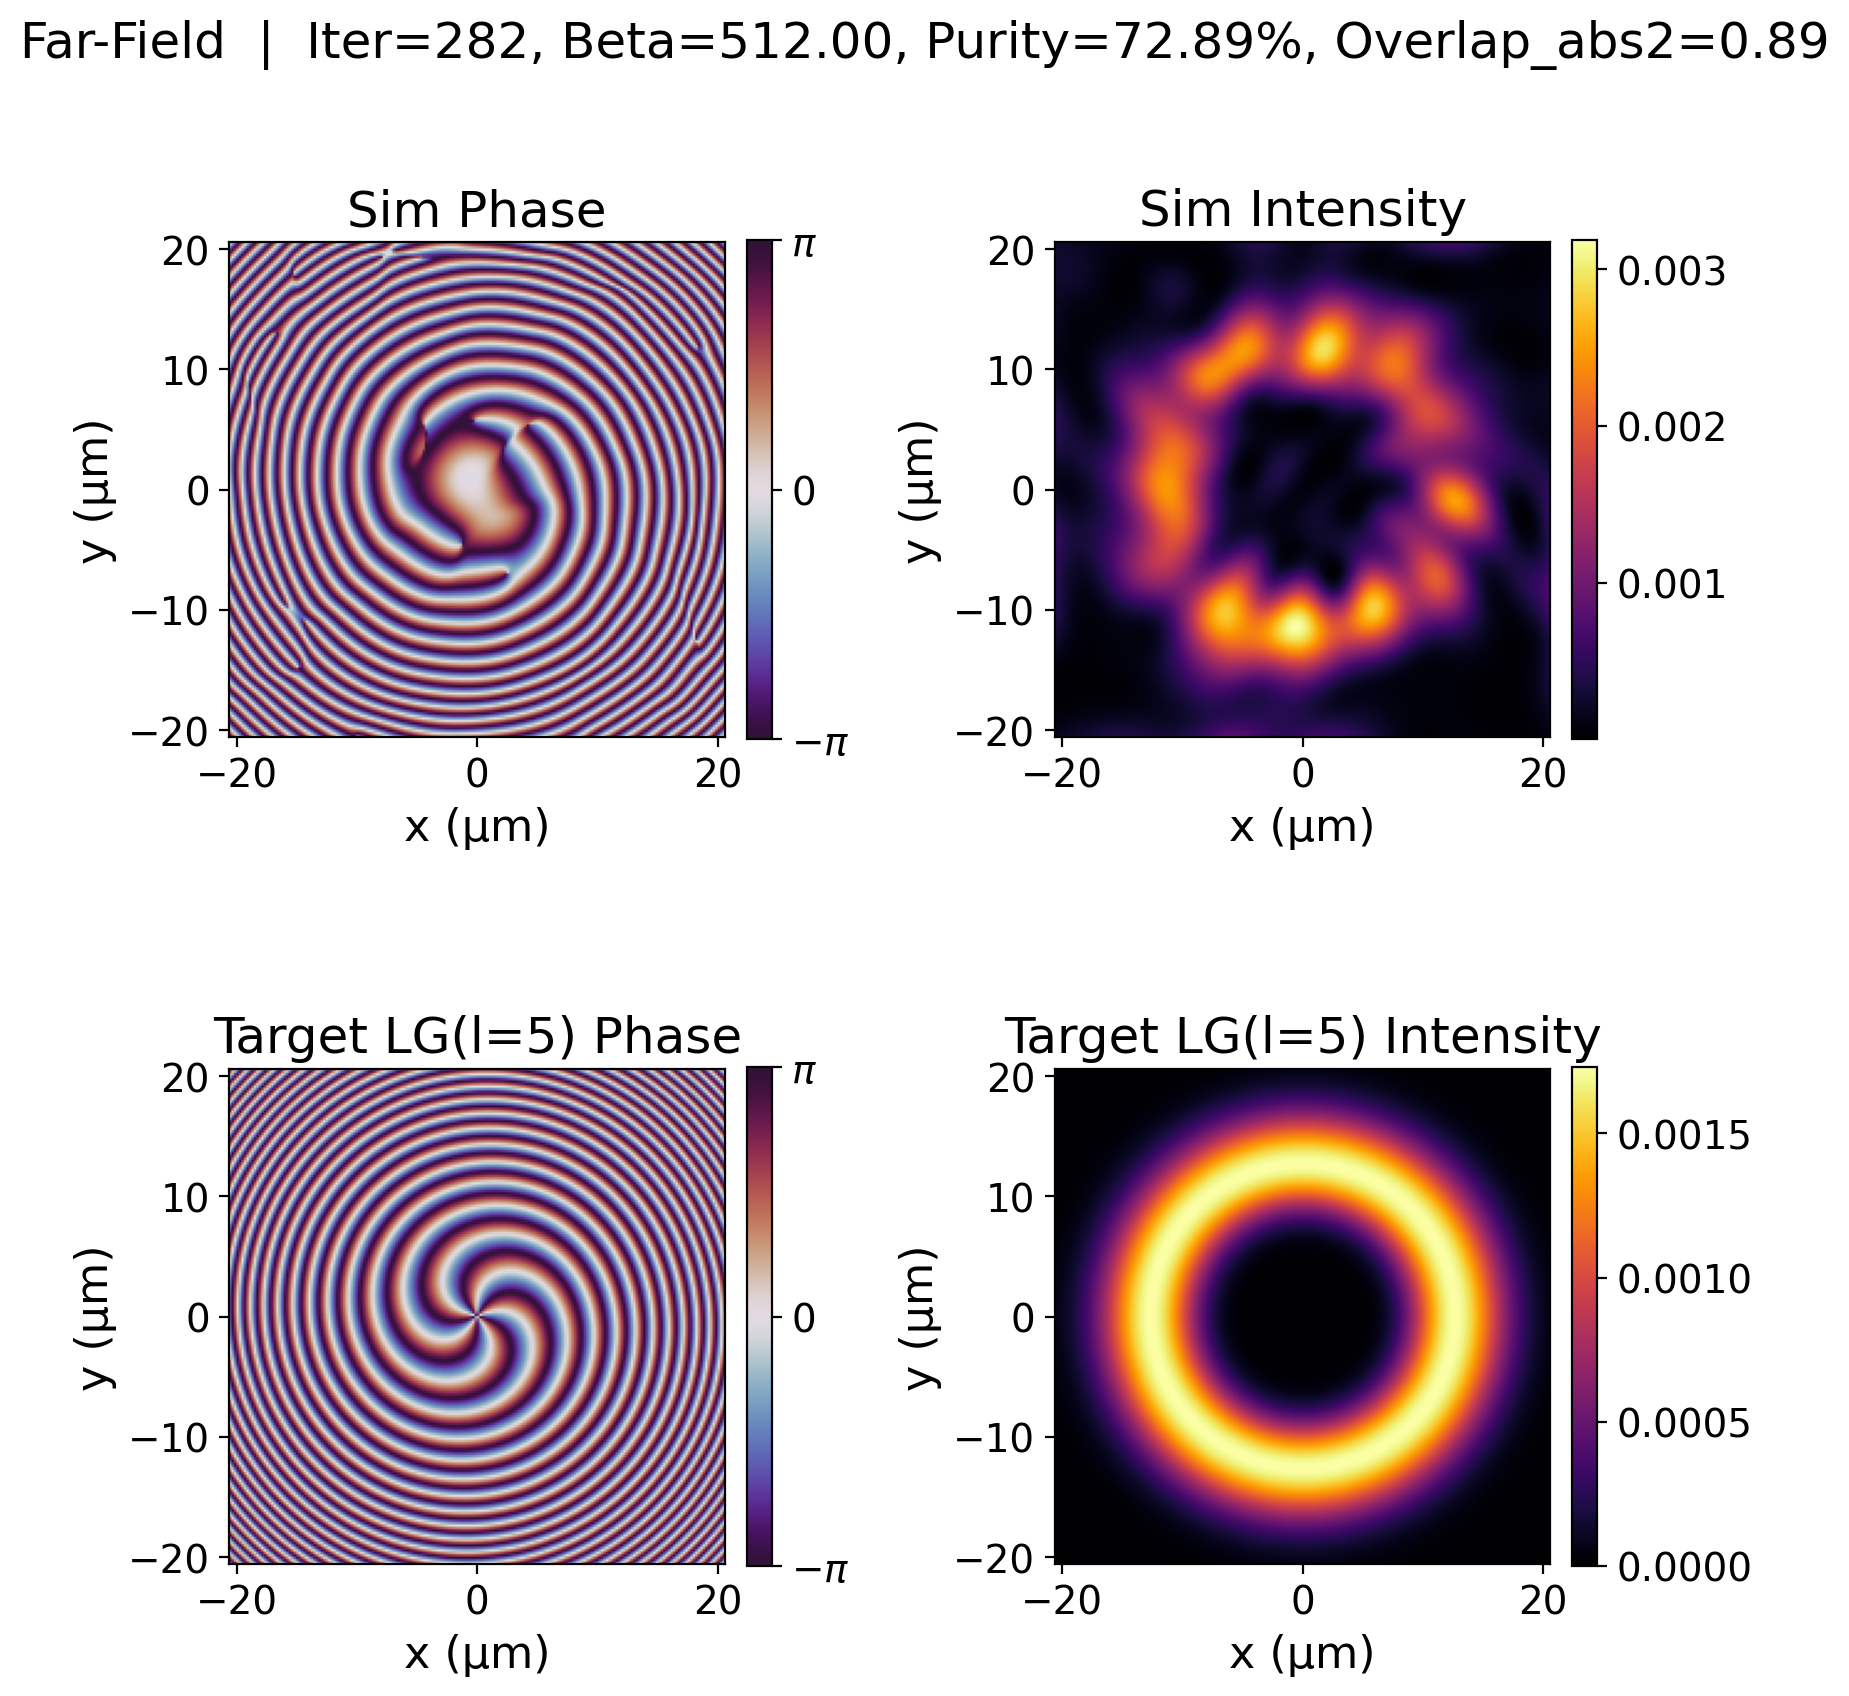
\includegraphics[width=1.0\linewidth,height=5.0cm,keepaspectratio]{img/016_ff_iter_282_beta_512.00.png} &
    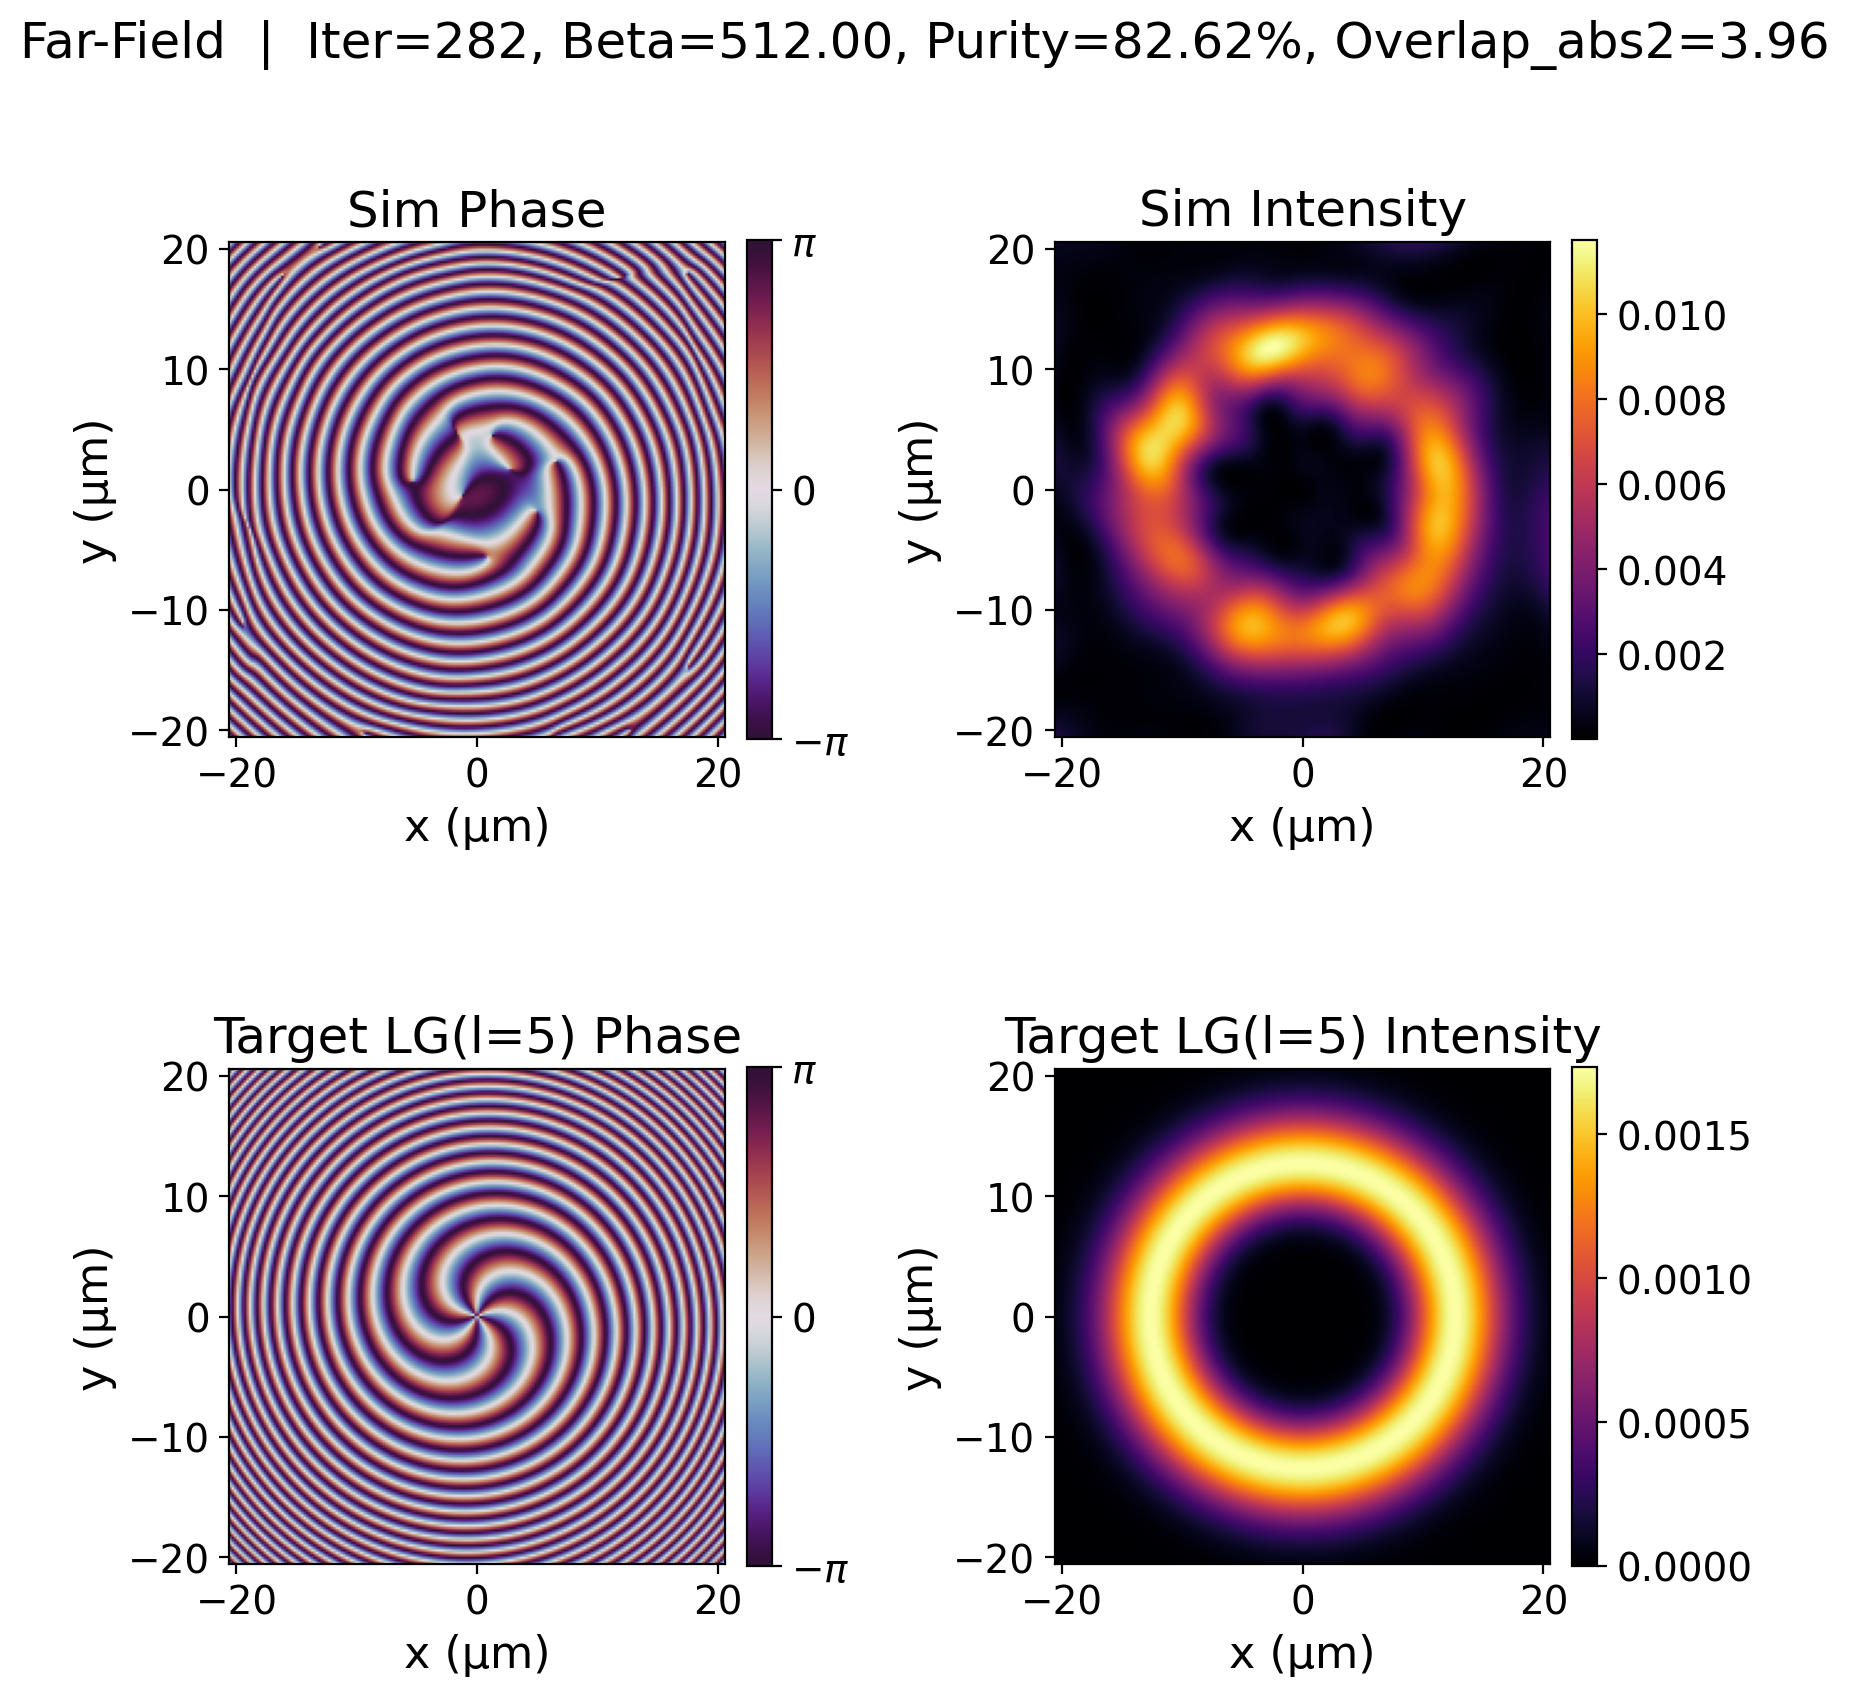
\includegraphics[width=1.0\linewidth,height=5.0cm,keepaspectratio]{img/022_ff_iter_282_beta_512.00.png} \\
    {\small (a) FoM I =$\dfrac{|\text{Overlap}|^{2}}{P_\text{sim} P_\text{target}}$} & {\small (b) FoM II = $\log \dfrac{|\text{Overlap}|^{2}}{P_\text{sim} P_\text{target}} +\alpha \log|\text{Overlap}|^2$}
    \end{tabular}
  \end{center}
\end{frame}

% [R-1] Structures

\begin{frame}{Optimized Structures ($\ell=0\sim5$)}
  \begin{center}
    {\footnotesize GaP/air binary ($\beta=512$): \textbf{black}=GaP, \textbf{white}=air}\\[1pt]
    \begin{tabular}{ccc}
    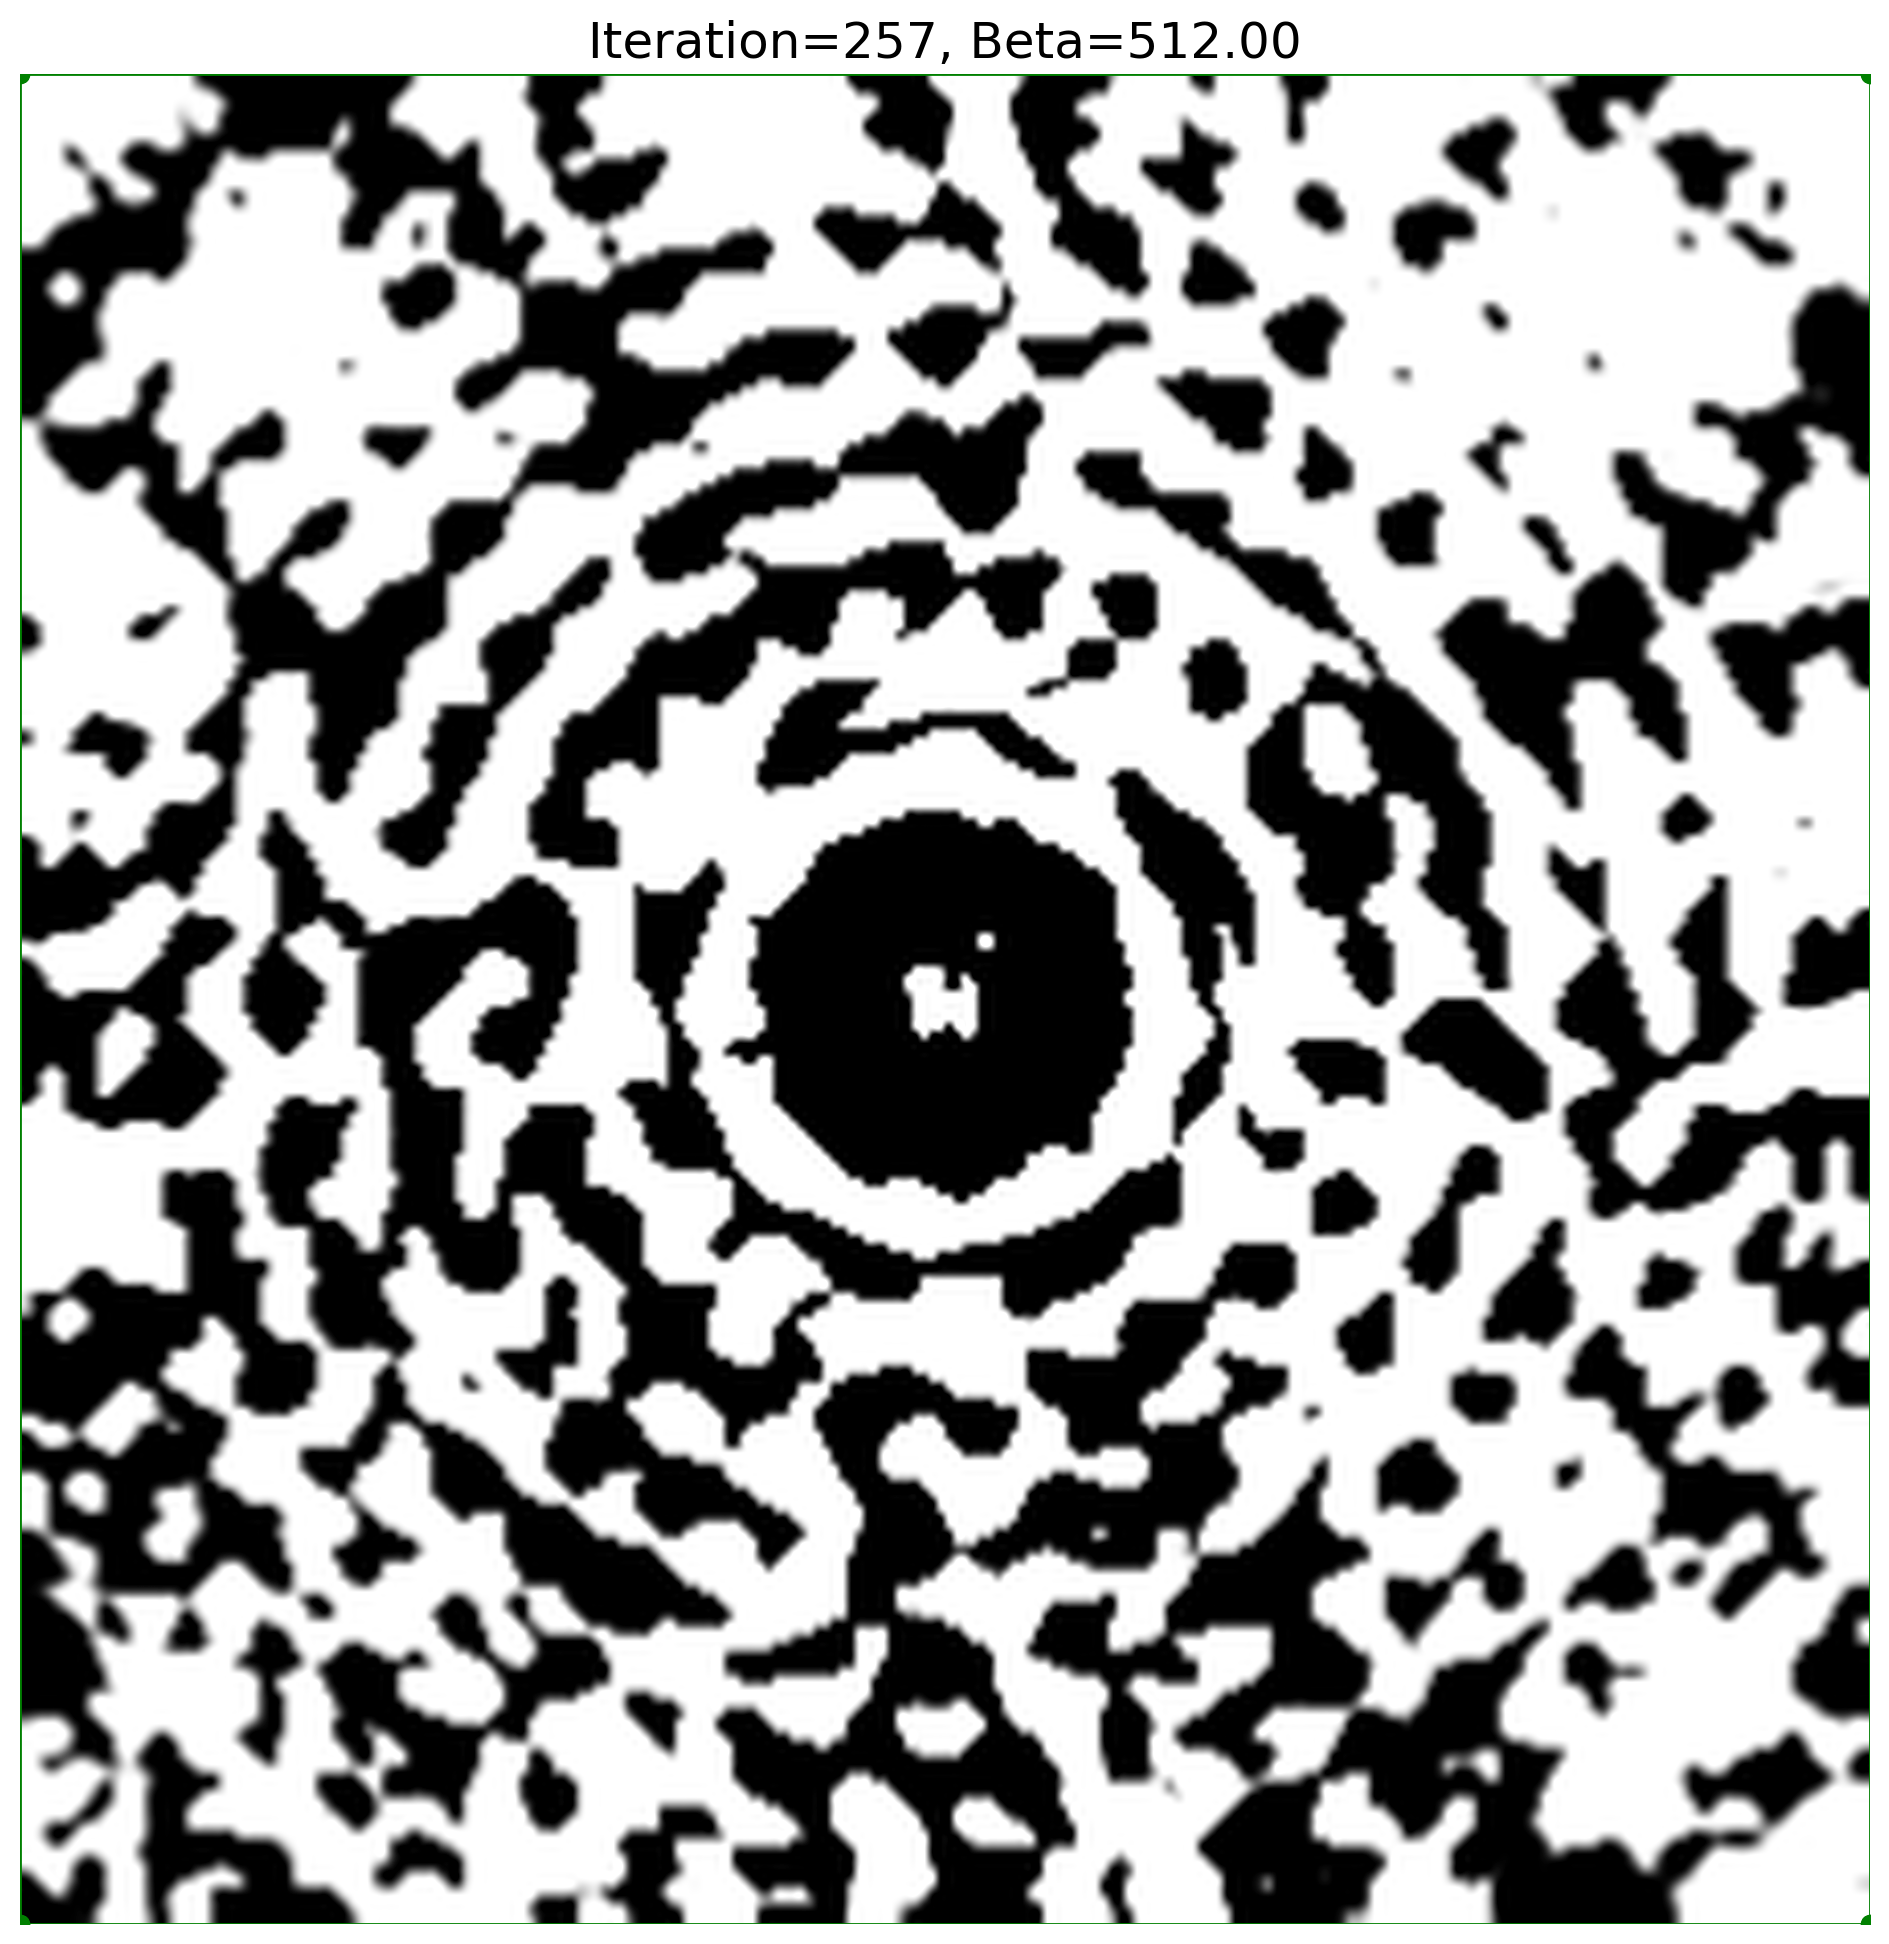
\includegraphics[width=0.31\linewidth,height=3.0cm,keepaspectratio]{img/017_structure_iter_257_beta_512.00.png} &
    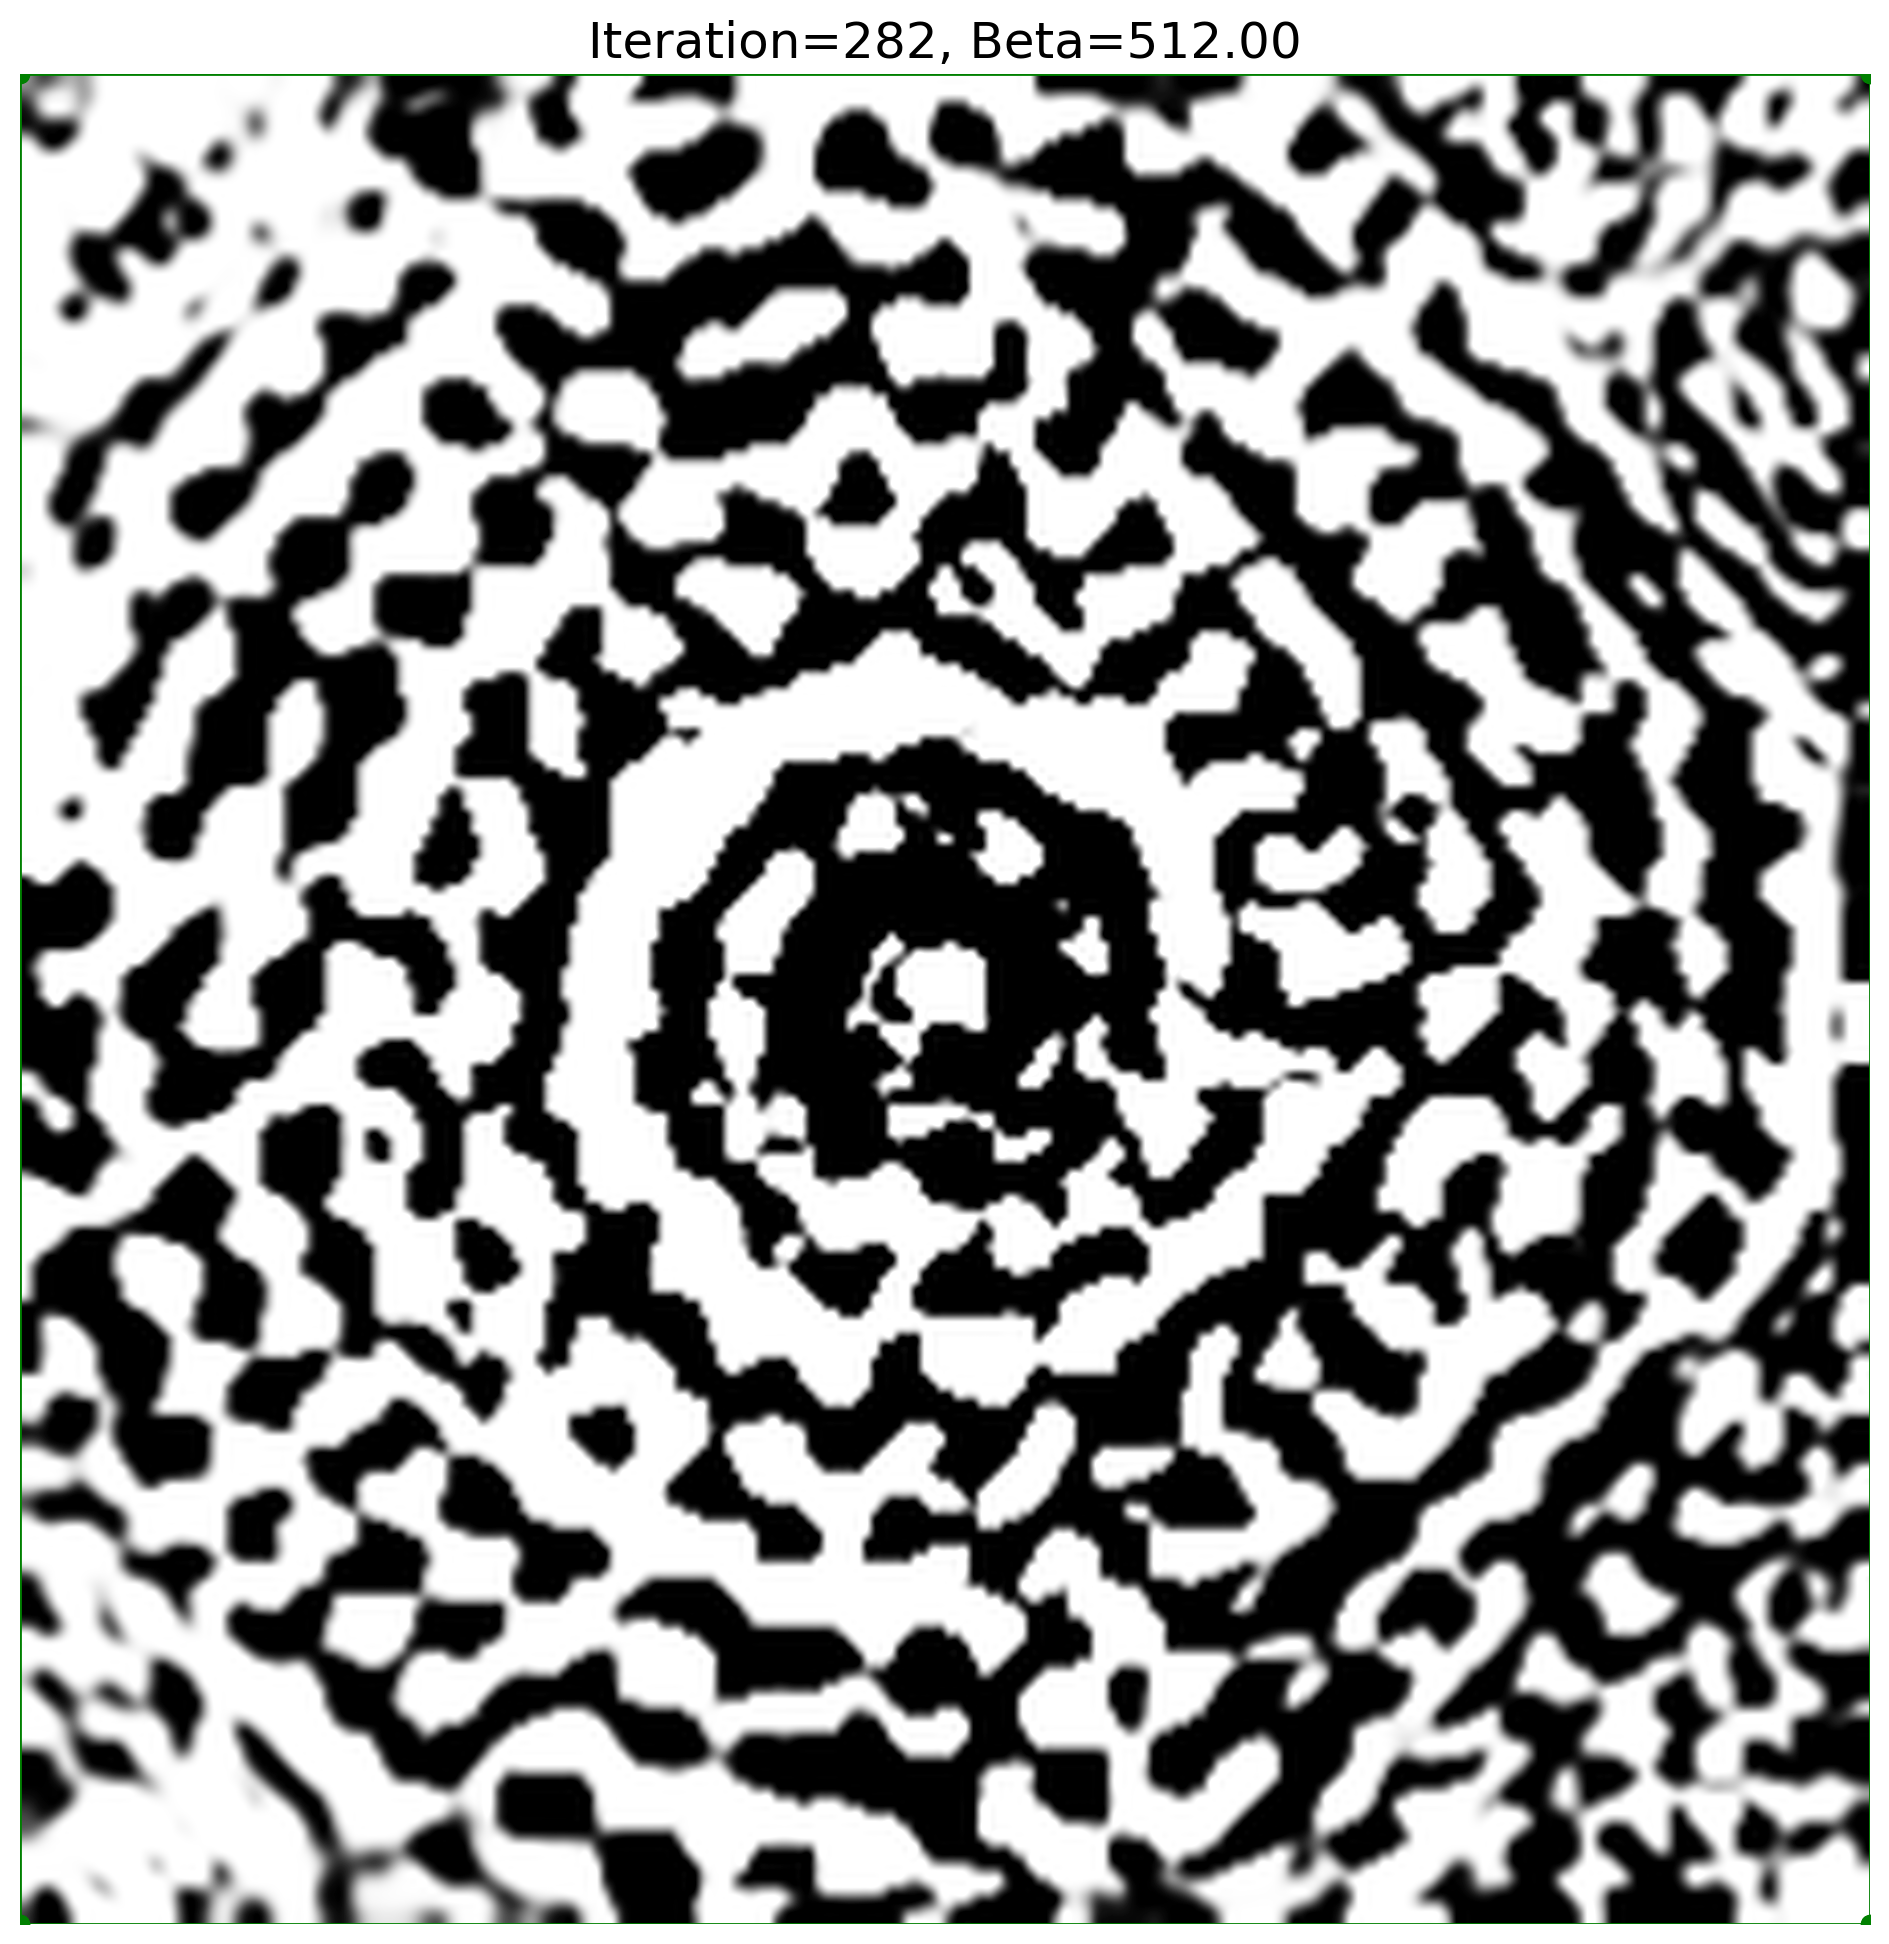
\includegraphics[width=0.31\linewidth,height=3.0cm,keepaspectratio]{img/018_structure_iter_282_beta_512.00.png} &
    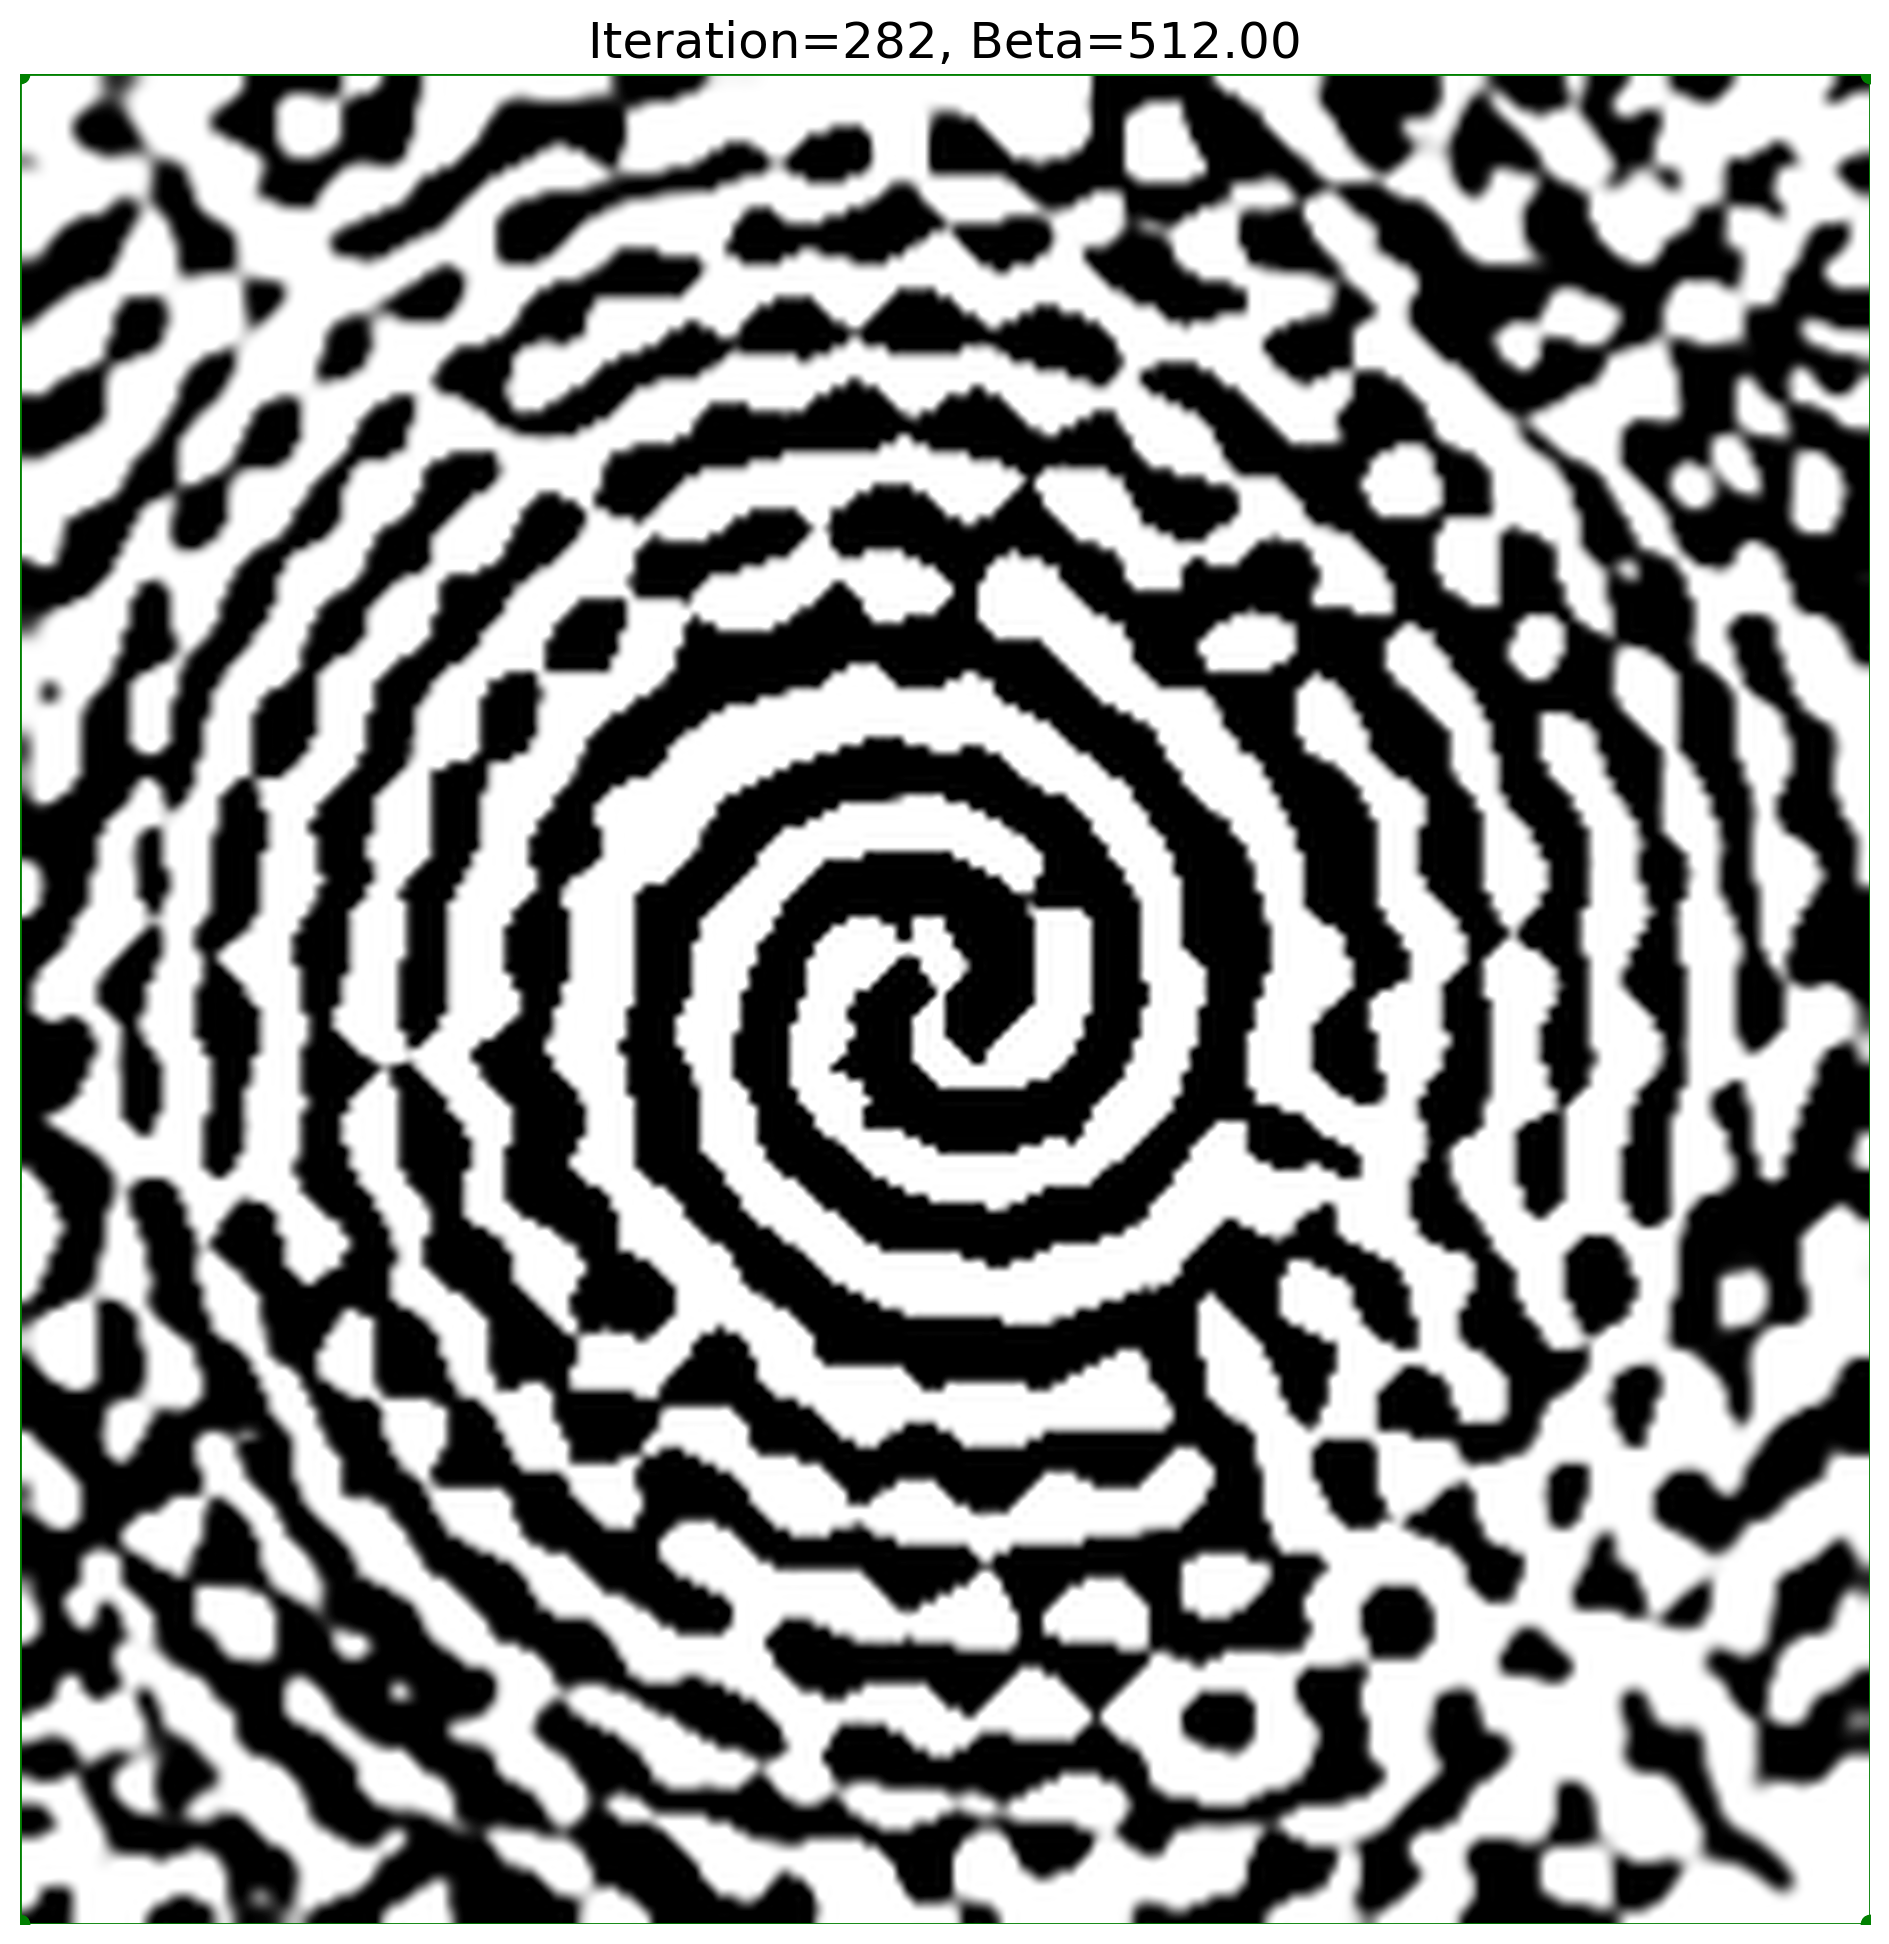
\includegraphics[width=0.31\linewidth,height=3.0cm,keepaspectratio]{img/013_structure_iter_282_beta_512.00.png} \\
    {\small (a) $\ell=0$} & {\small (b) $\ell=1$} & {\small (c) $\ell=2$}\\[1pt]
	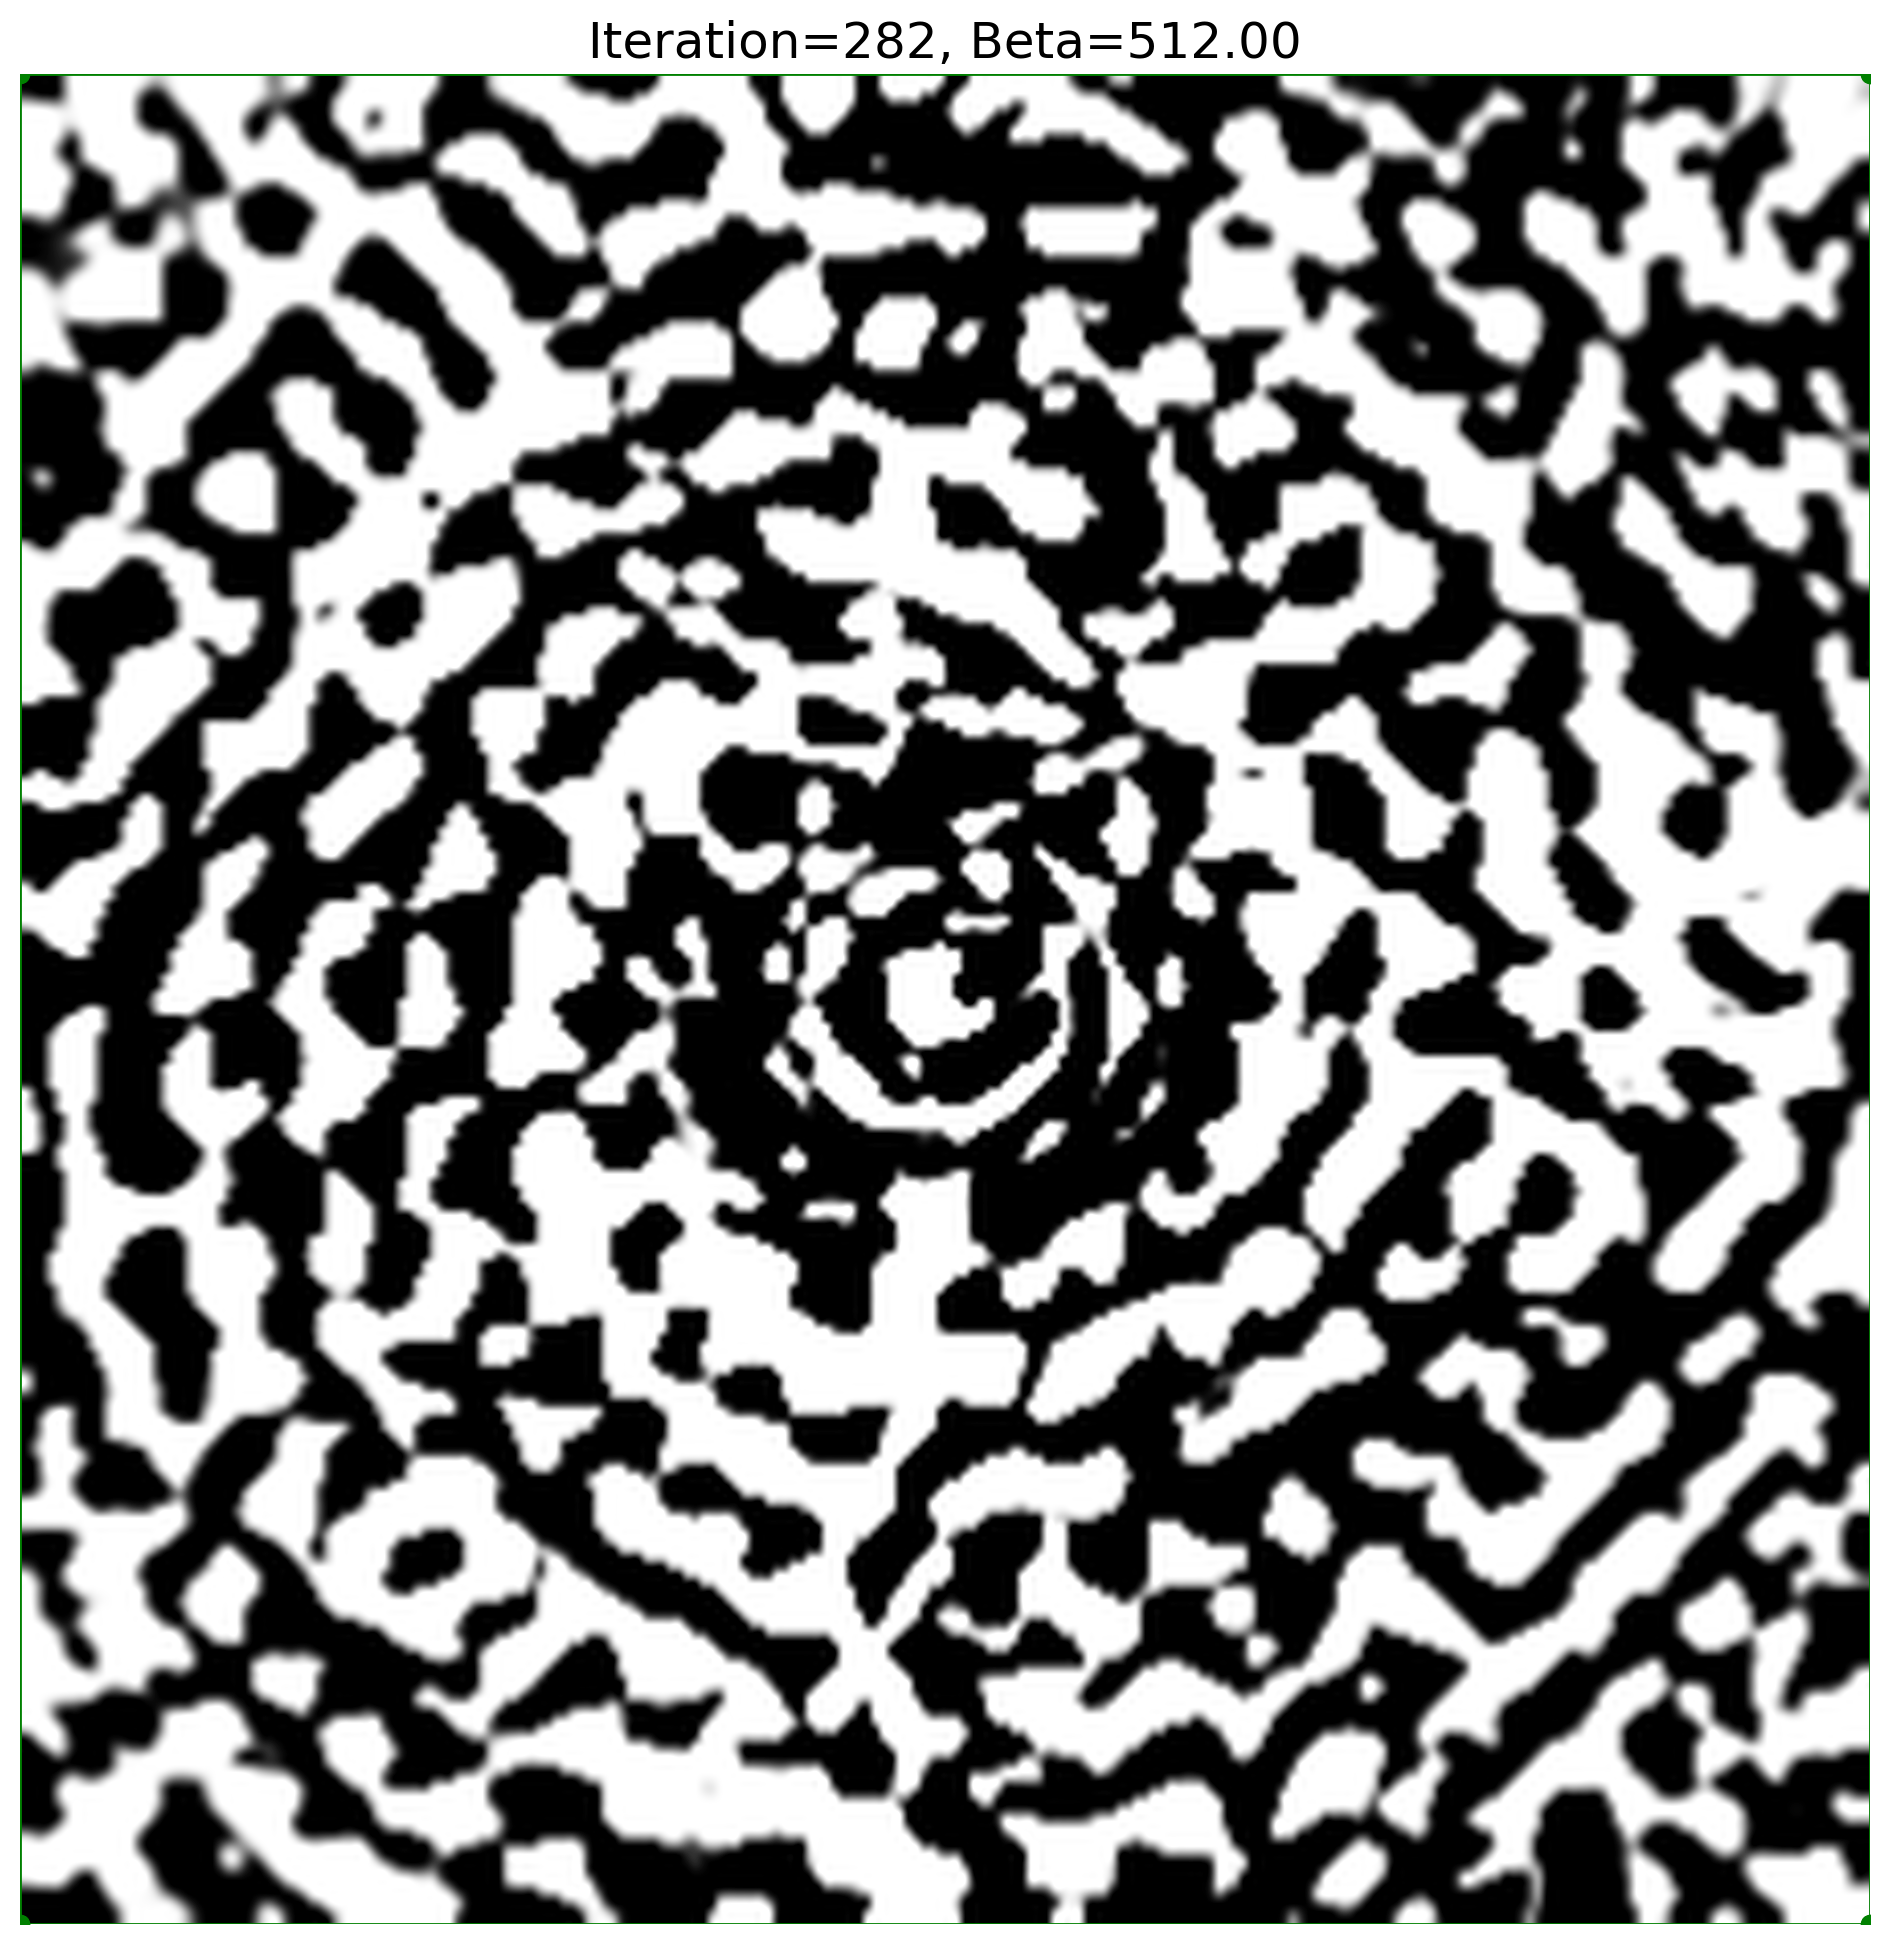
\includegraphics[width=0.31\linewidth,height=3.0cm,keepaspectratio]{img/020_structure_iter_282_beta_512.00.png} &
    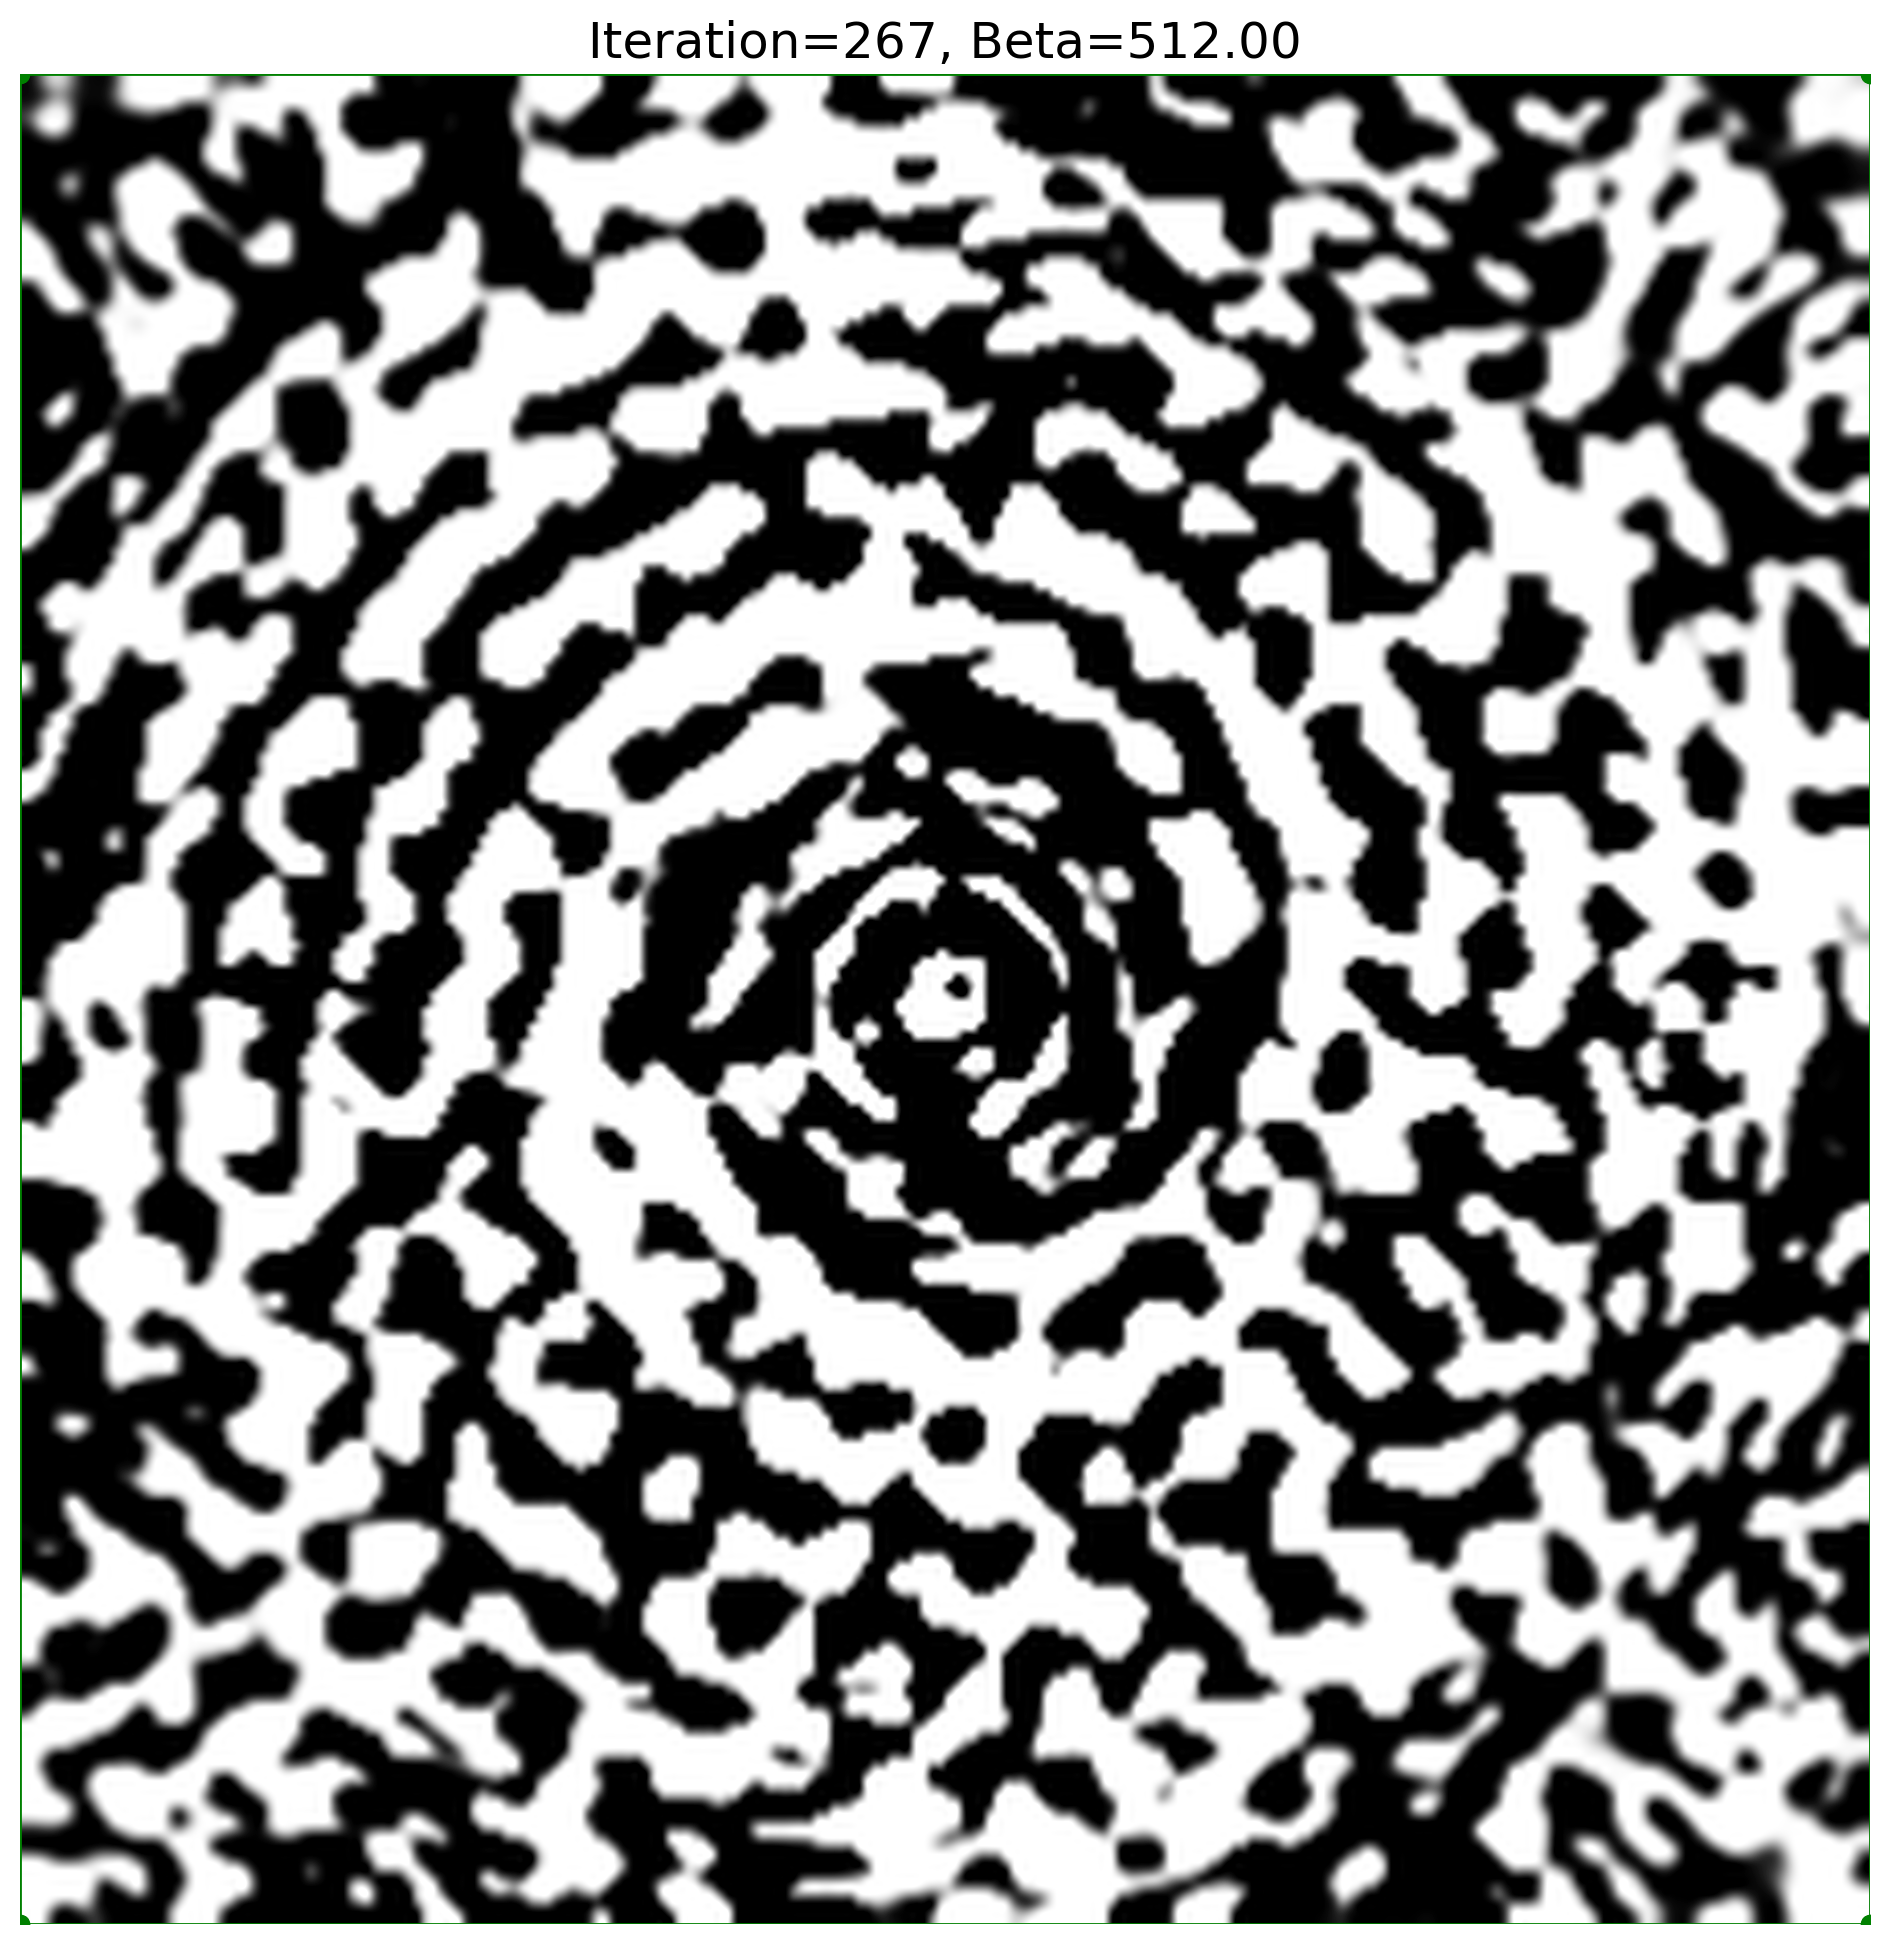
\includegraphics[width=0.31\linewidth,height=3.0cm,keepaspectratio]{img/021_structure_iter_267_beta_512.00.png} &
    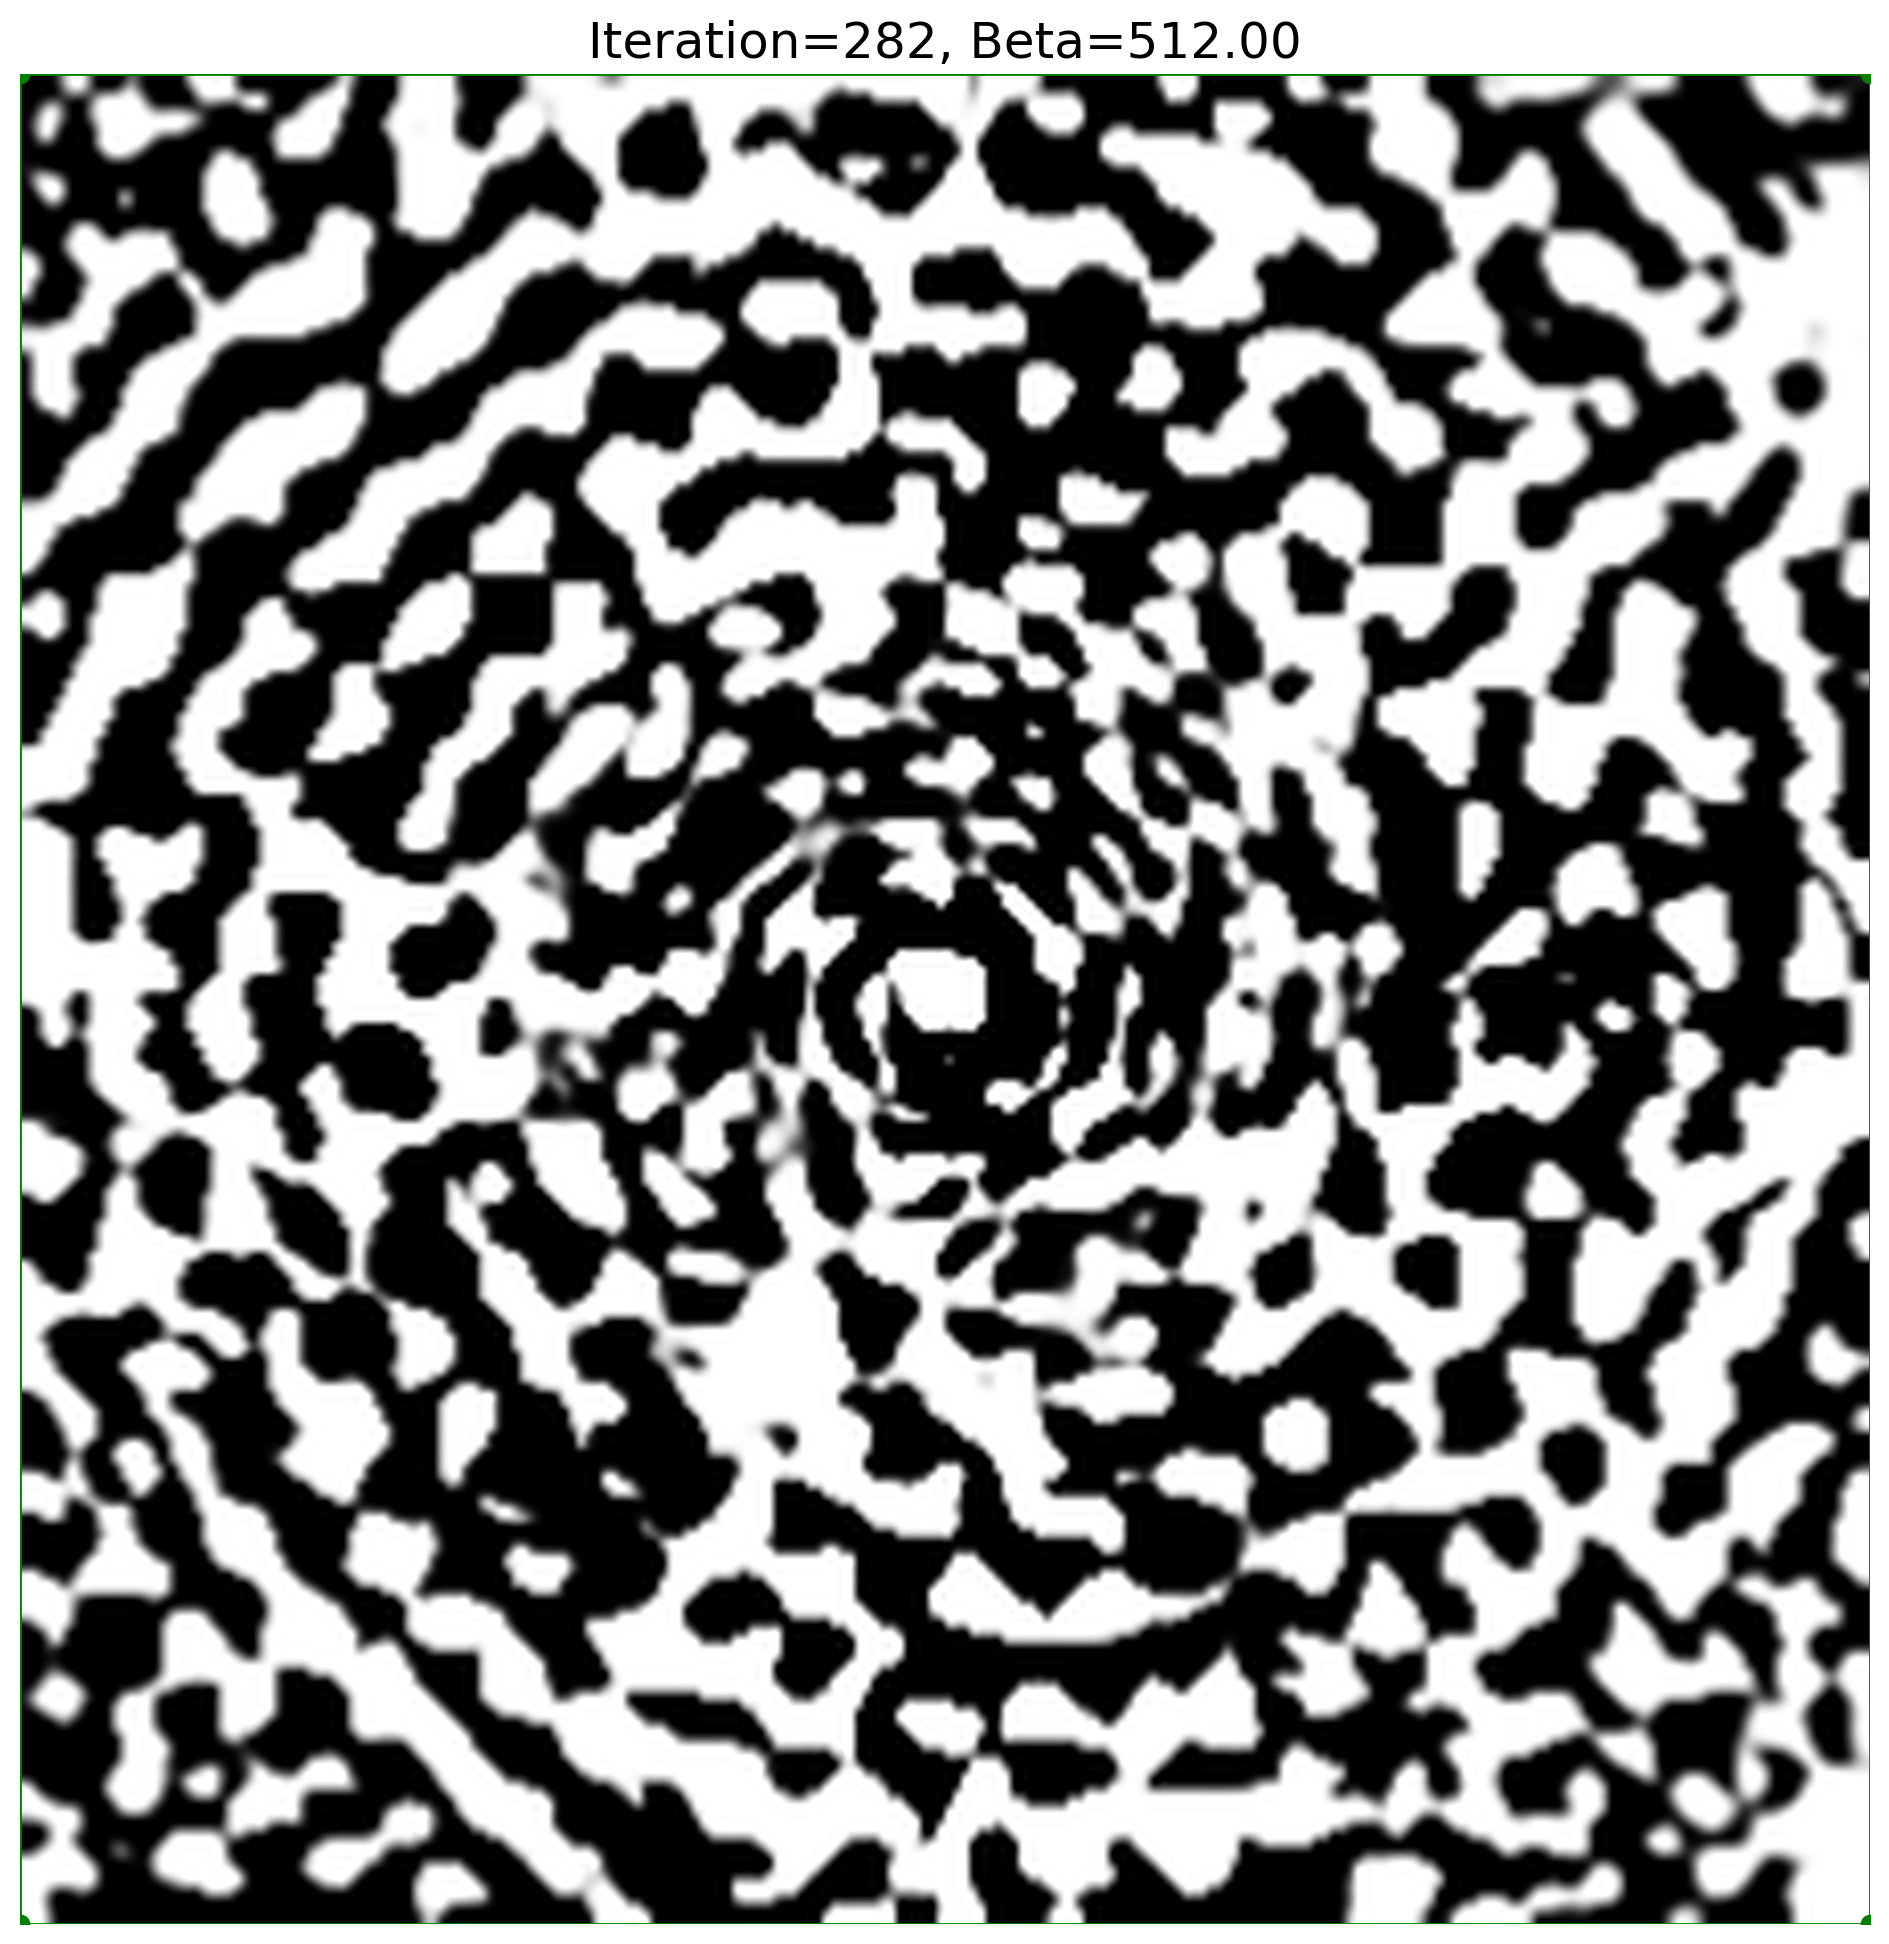
\includegraphics[width=0.31\linewidth,height=3.0cm,keepaspectratio]{img/022_structure_iter_282_beta_512.00.png} \\
    {\small (d) $\ell=3$} & {\small (e) $\ell=4$} & {\small (f) $\ell=5$}
    \end{tabular}
  \end{center}
\end{frame}




% [R-2] Far-Field: high-purity group

\begin{frame}{Far-Field LG Mode ($\ell=0,1,2,3$) at $z=10\,z_R$} 
\centering 
\begin{tabular}{cccc}
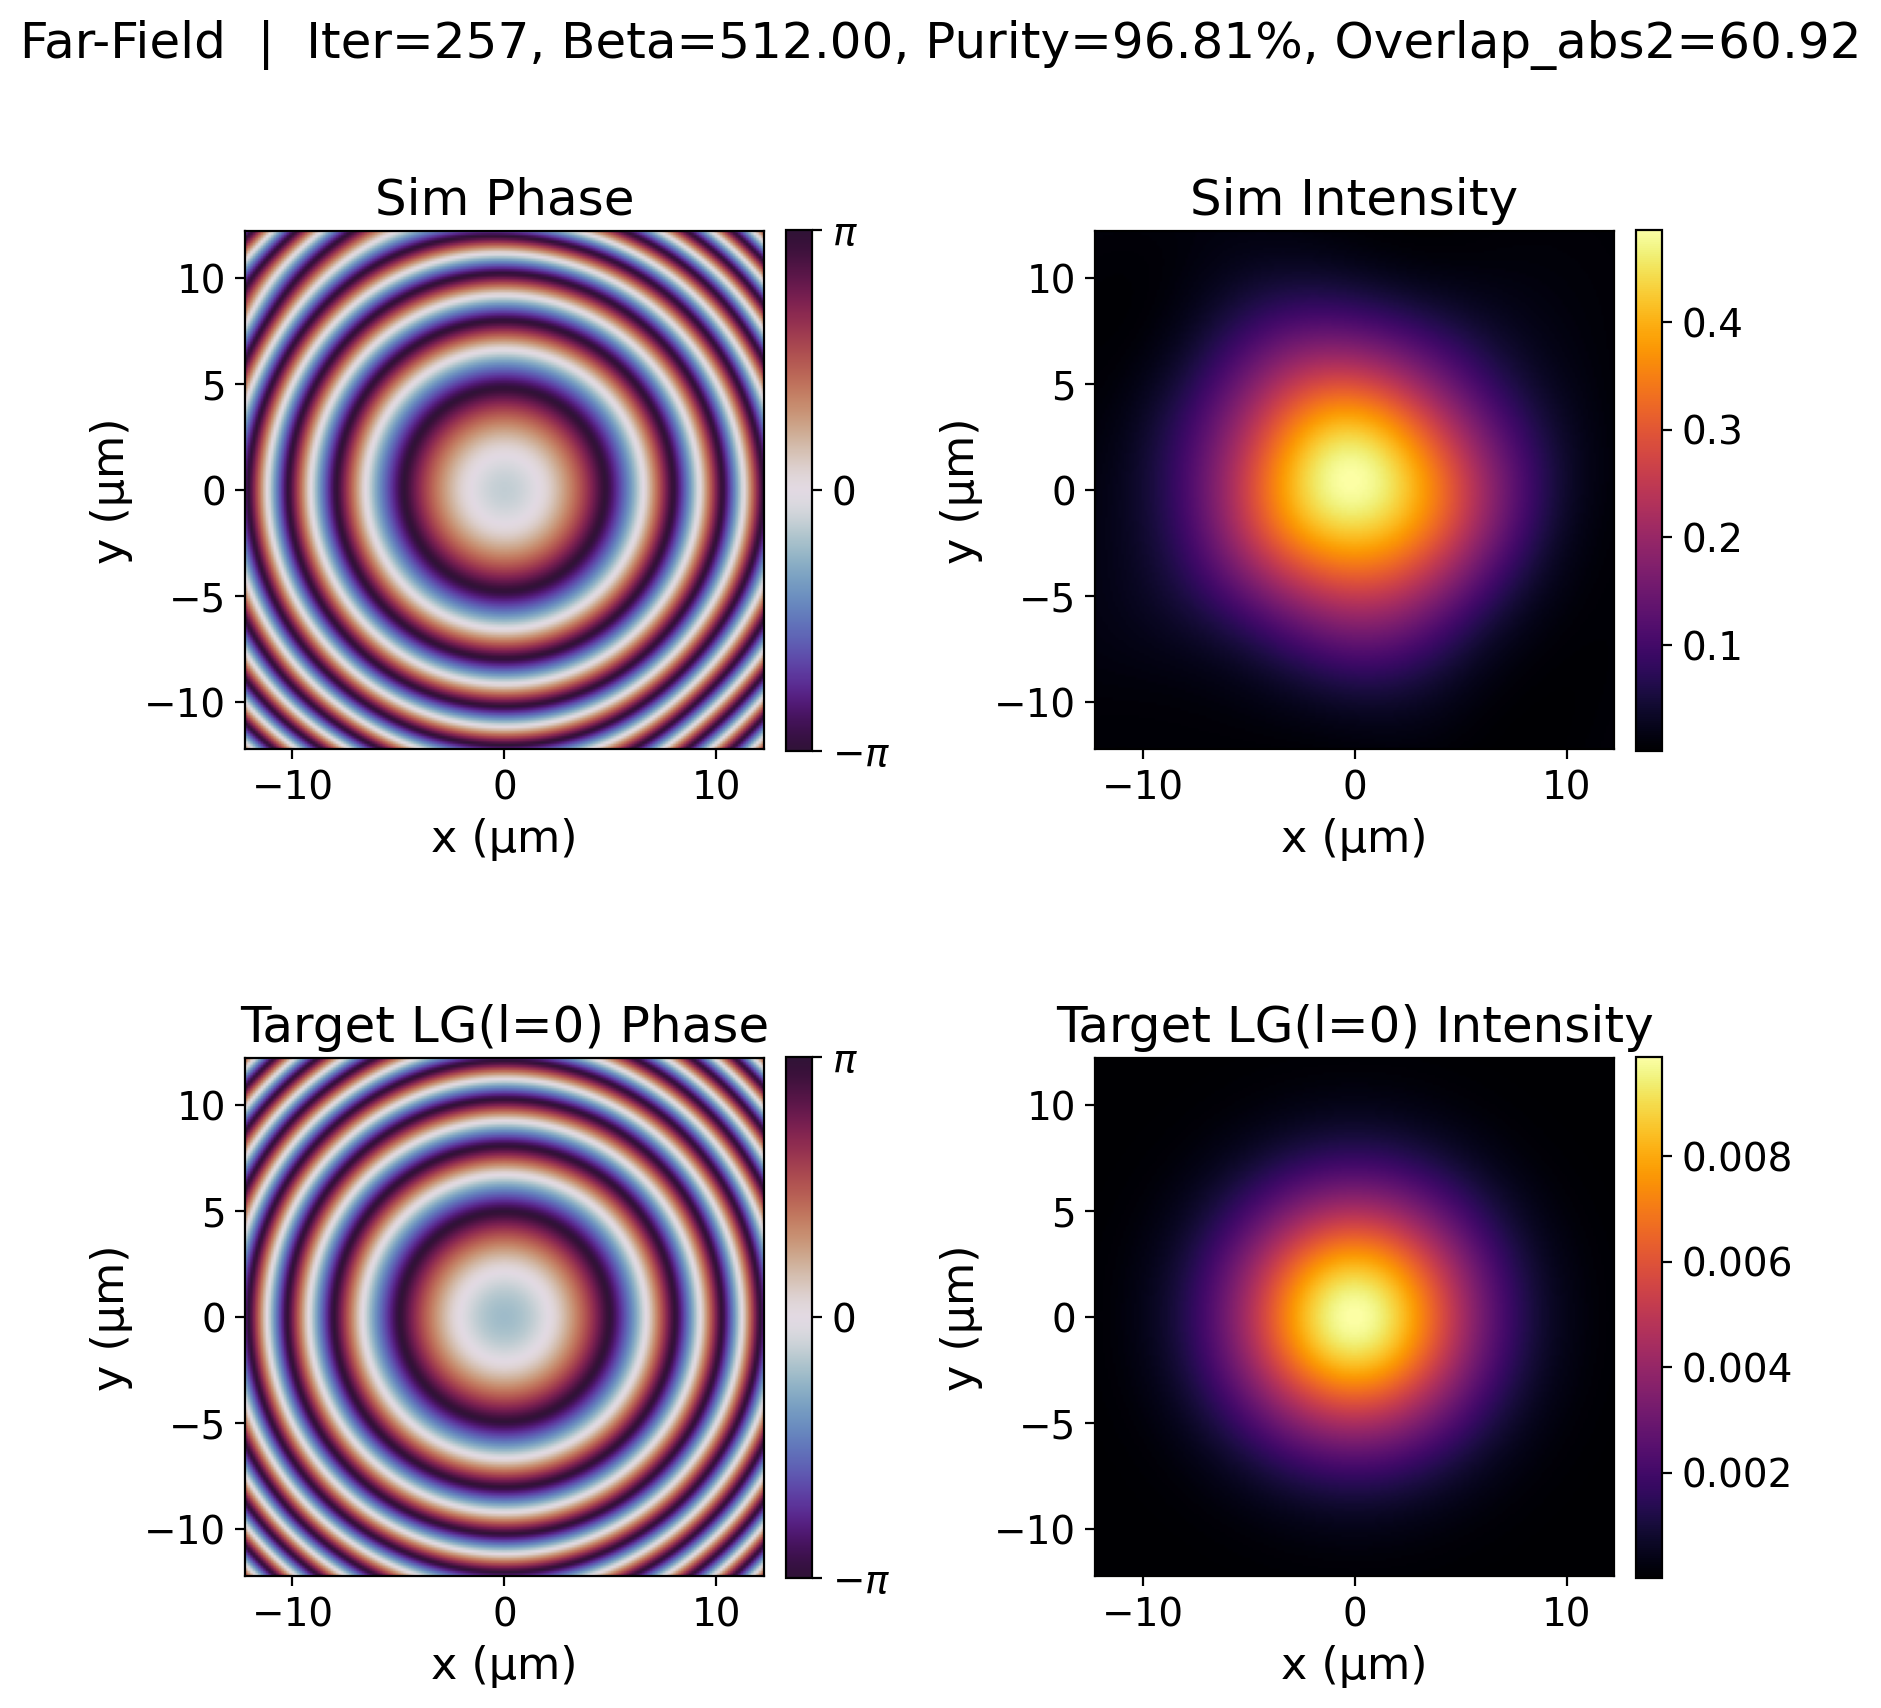
\includegraphics[width=0.23\textwidth,height=3.3cm,keepaspectratio]{img/017_ff_iter_257_beta_512.00.png} & 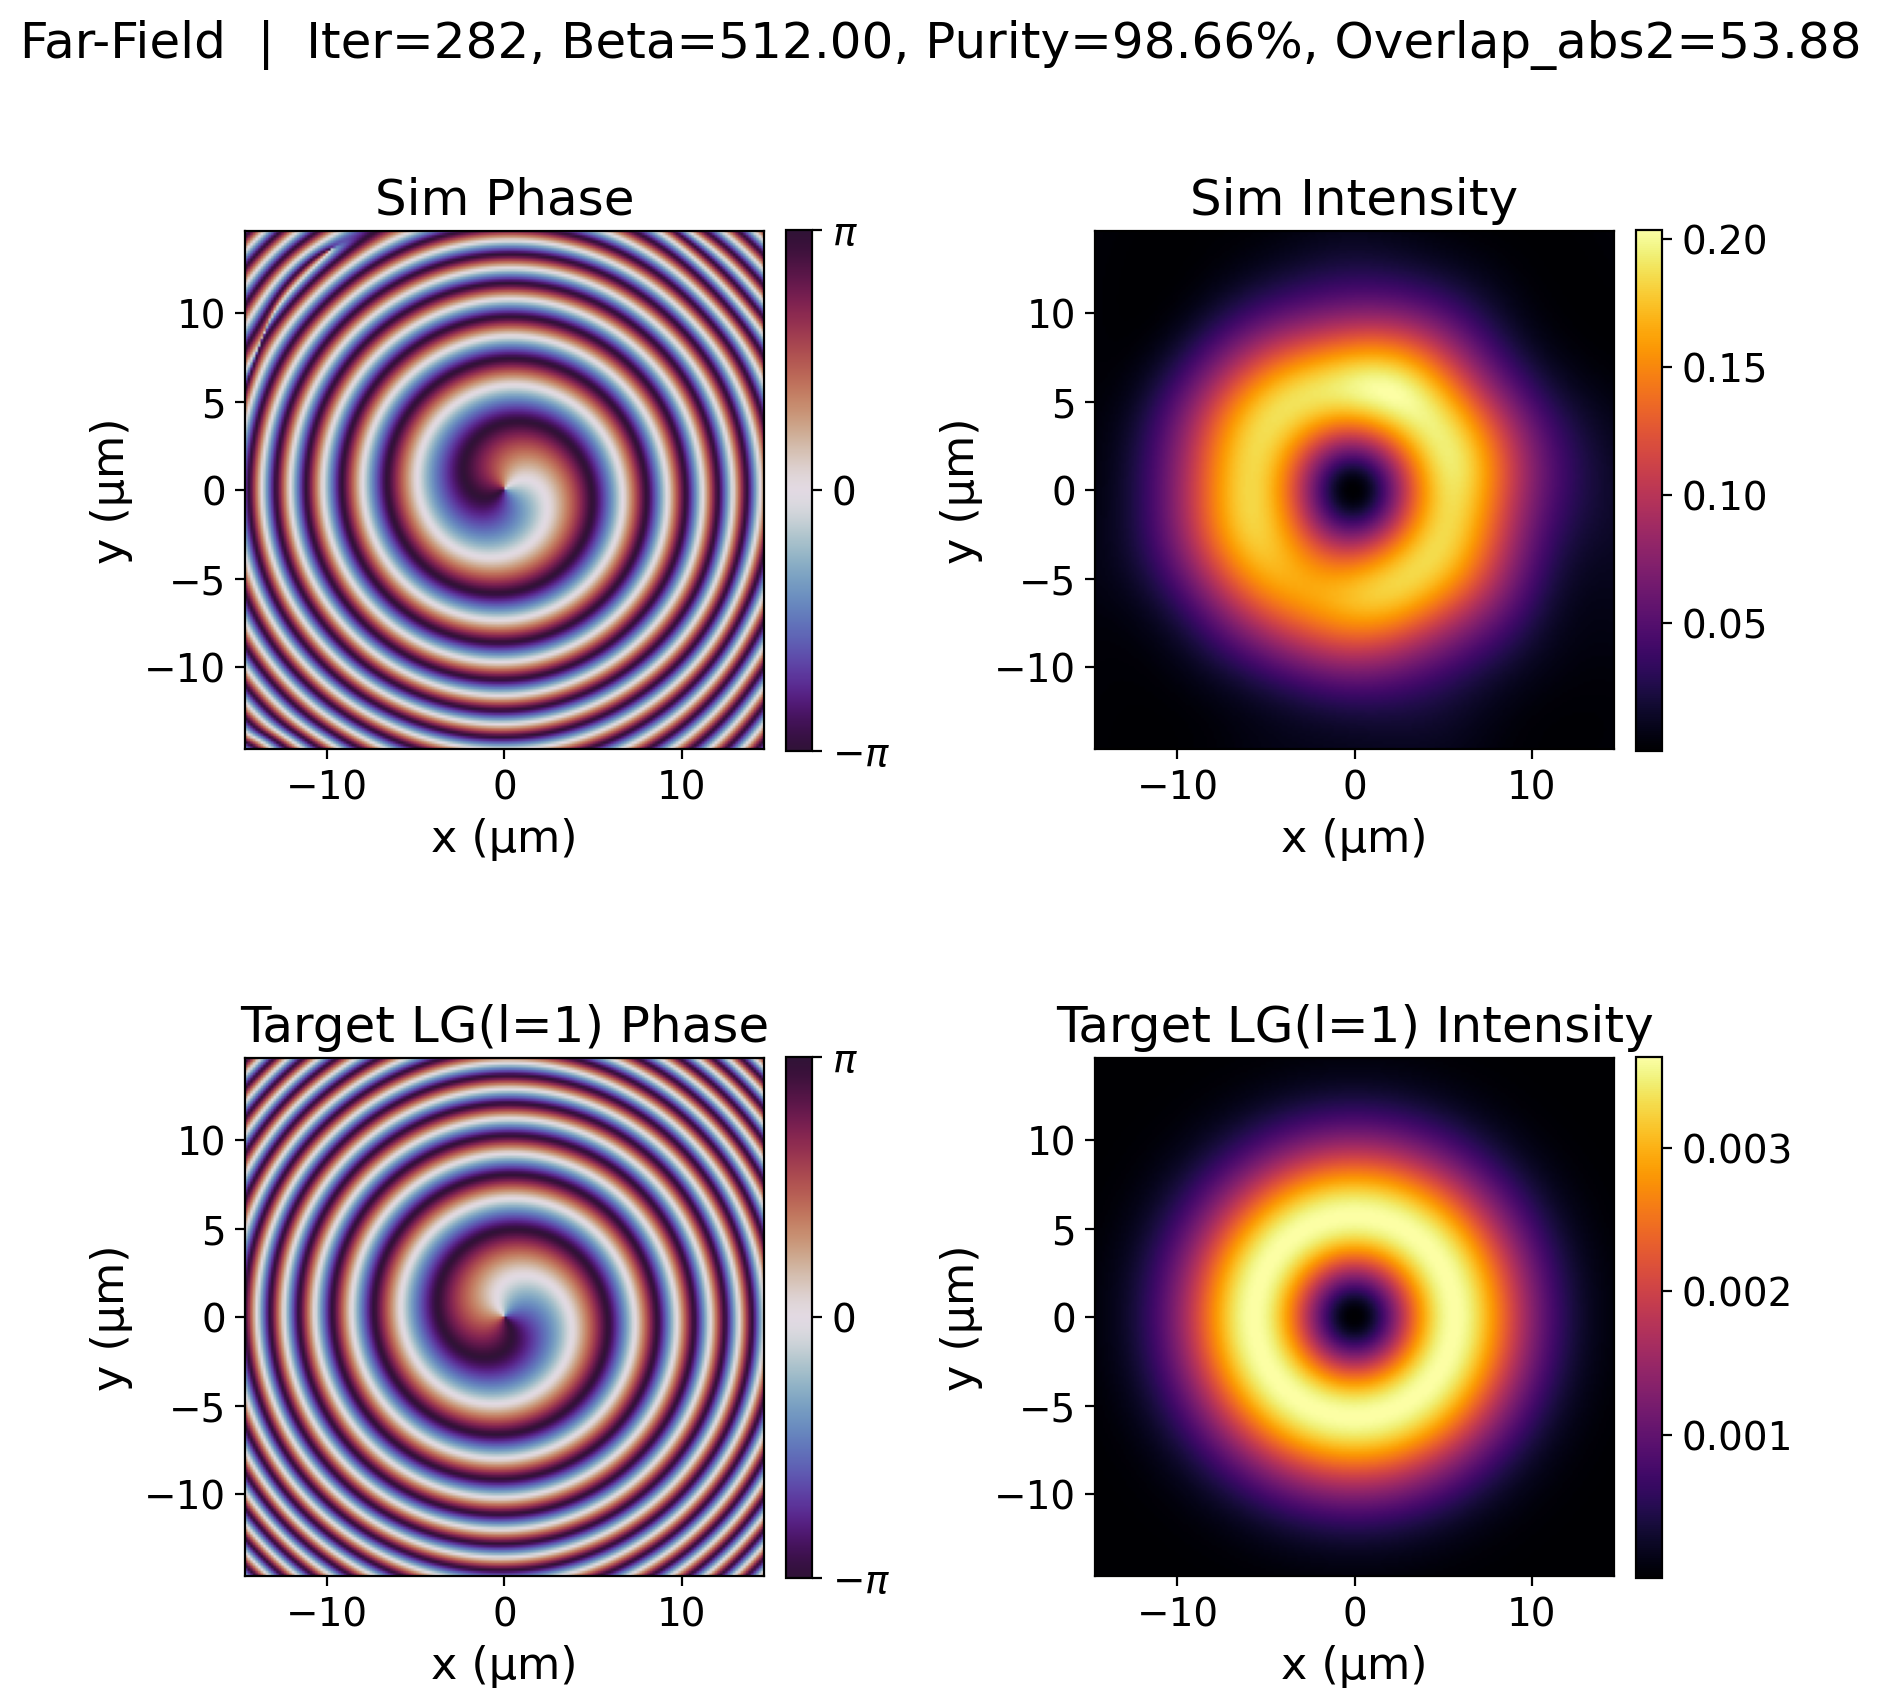
\includegraphics[width=0.23\textwidth,height=3.3cm,keepaspectratio]{img/018_ff_iter_282_beta_512.00.png} & 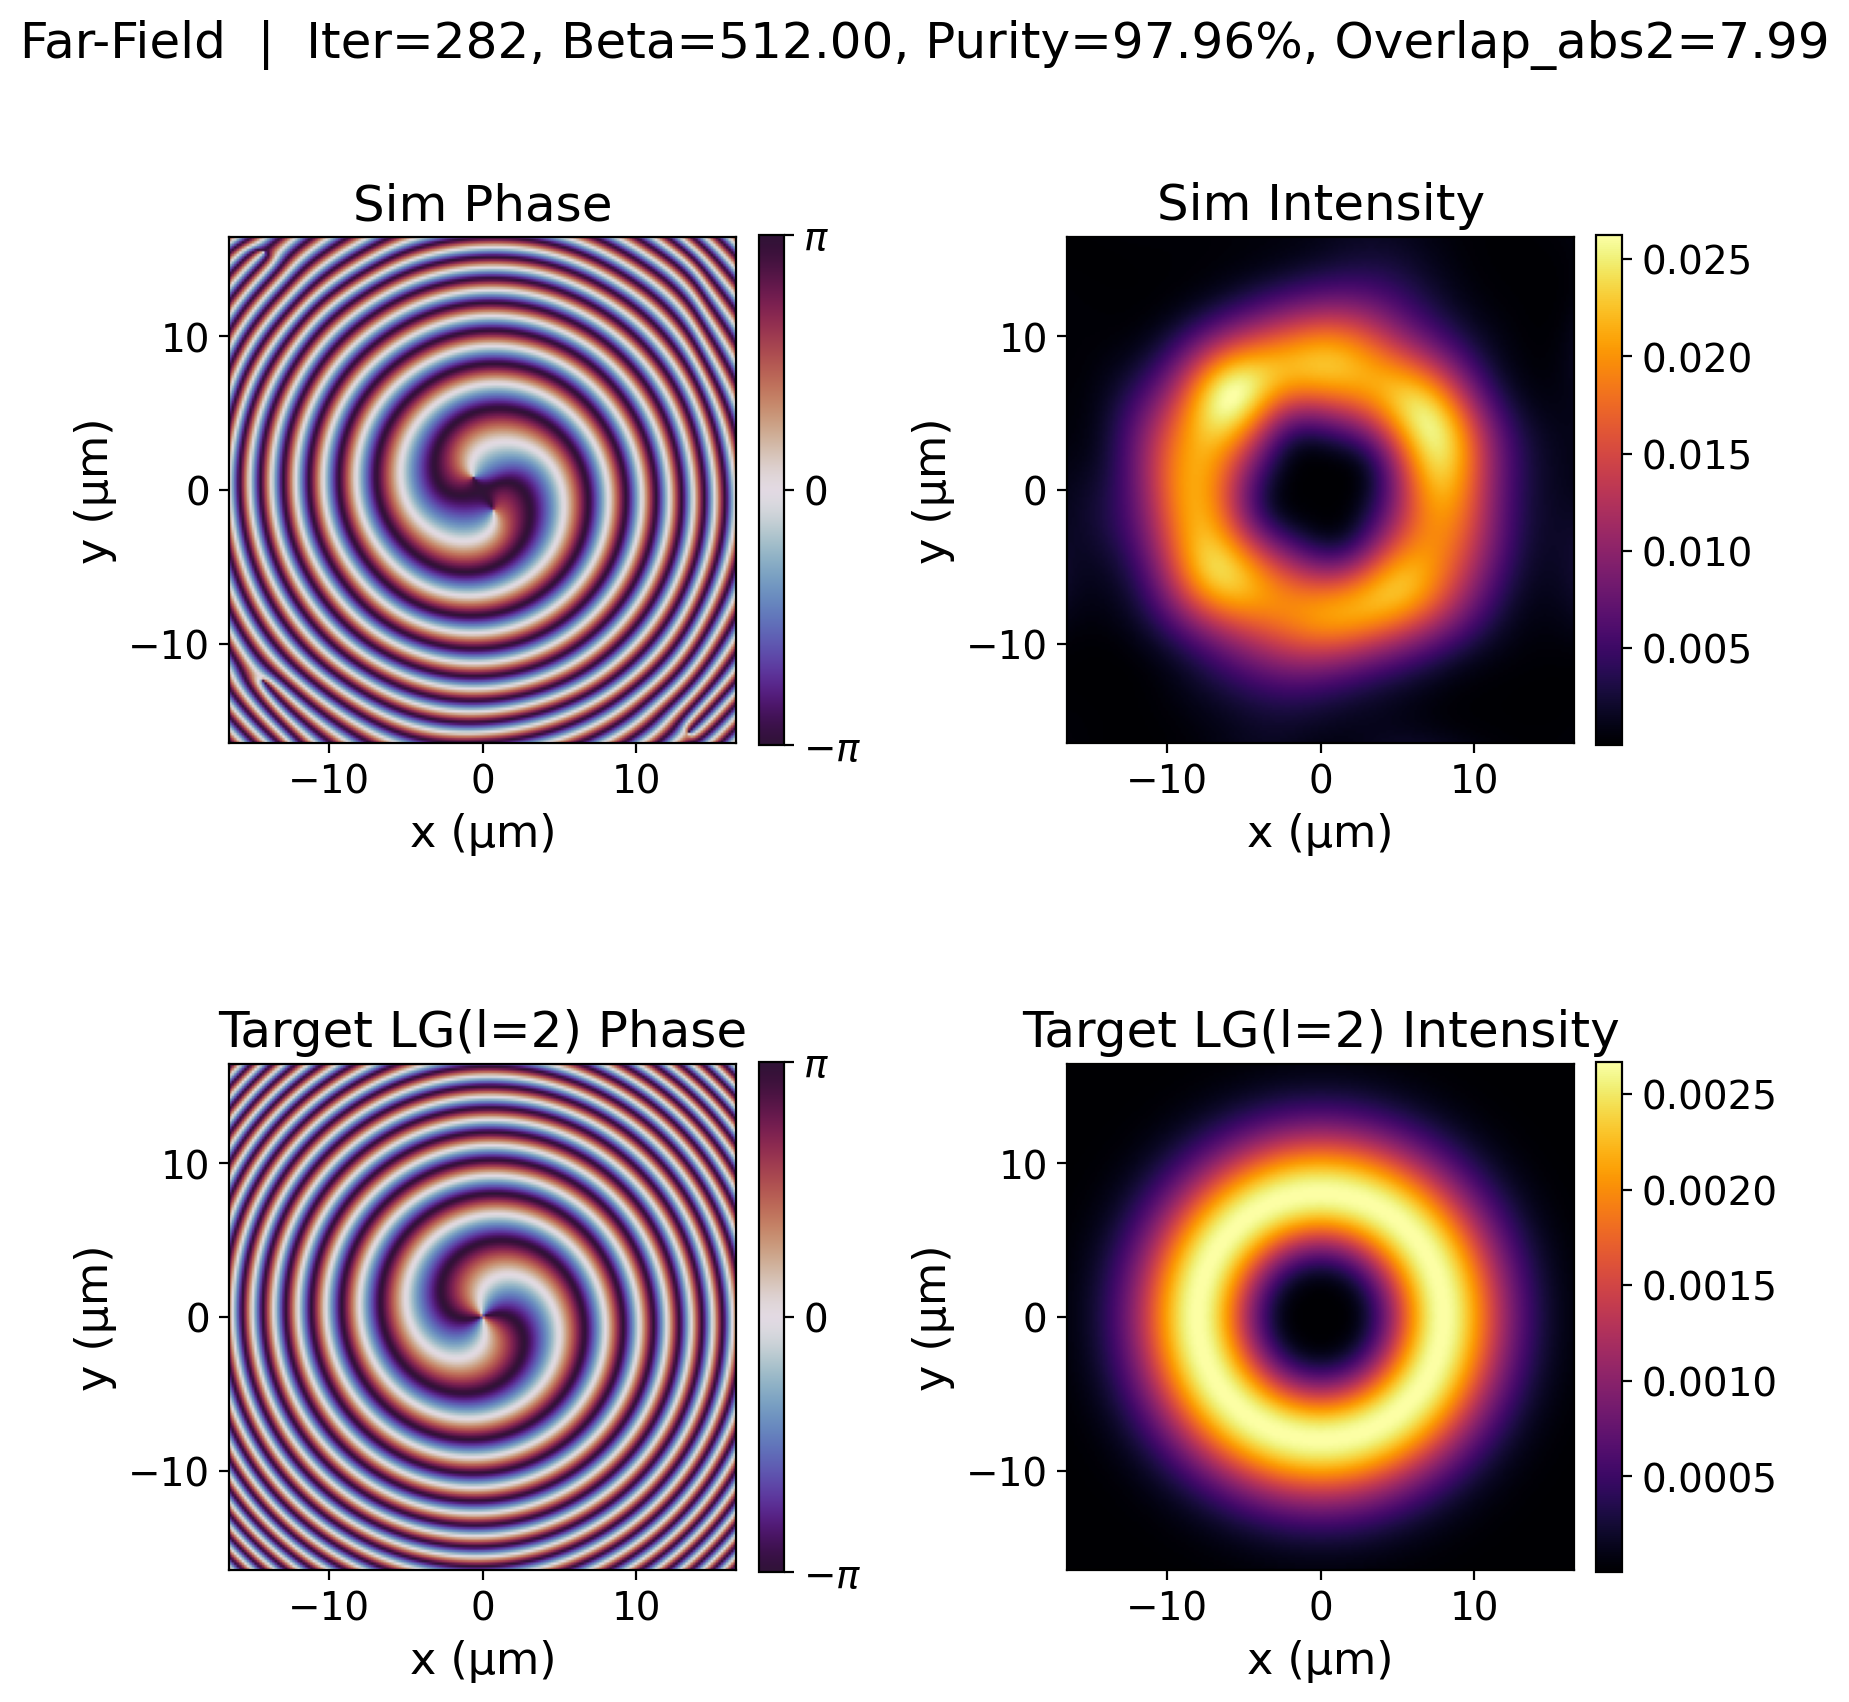
\includegraphics[width=0.23\textwidth,height=3.3cm,keepaspectratio]{img/013_ff_iter_282_beta_512.00.png} & 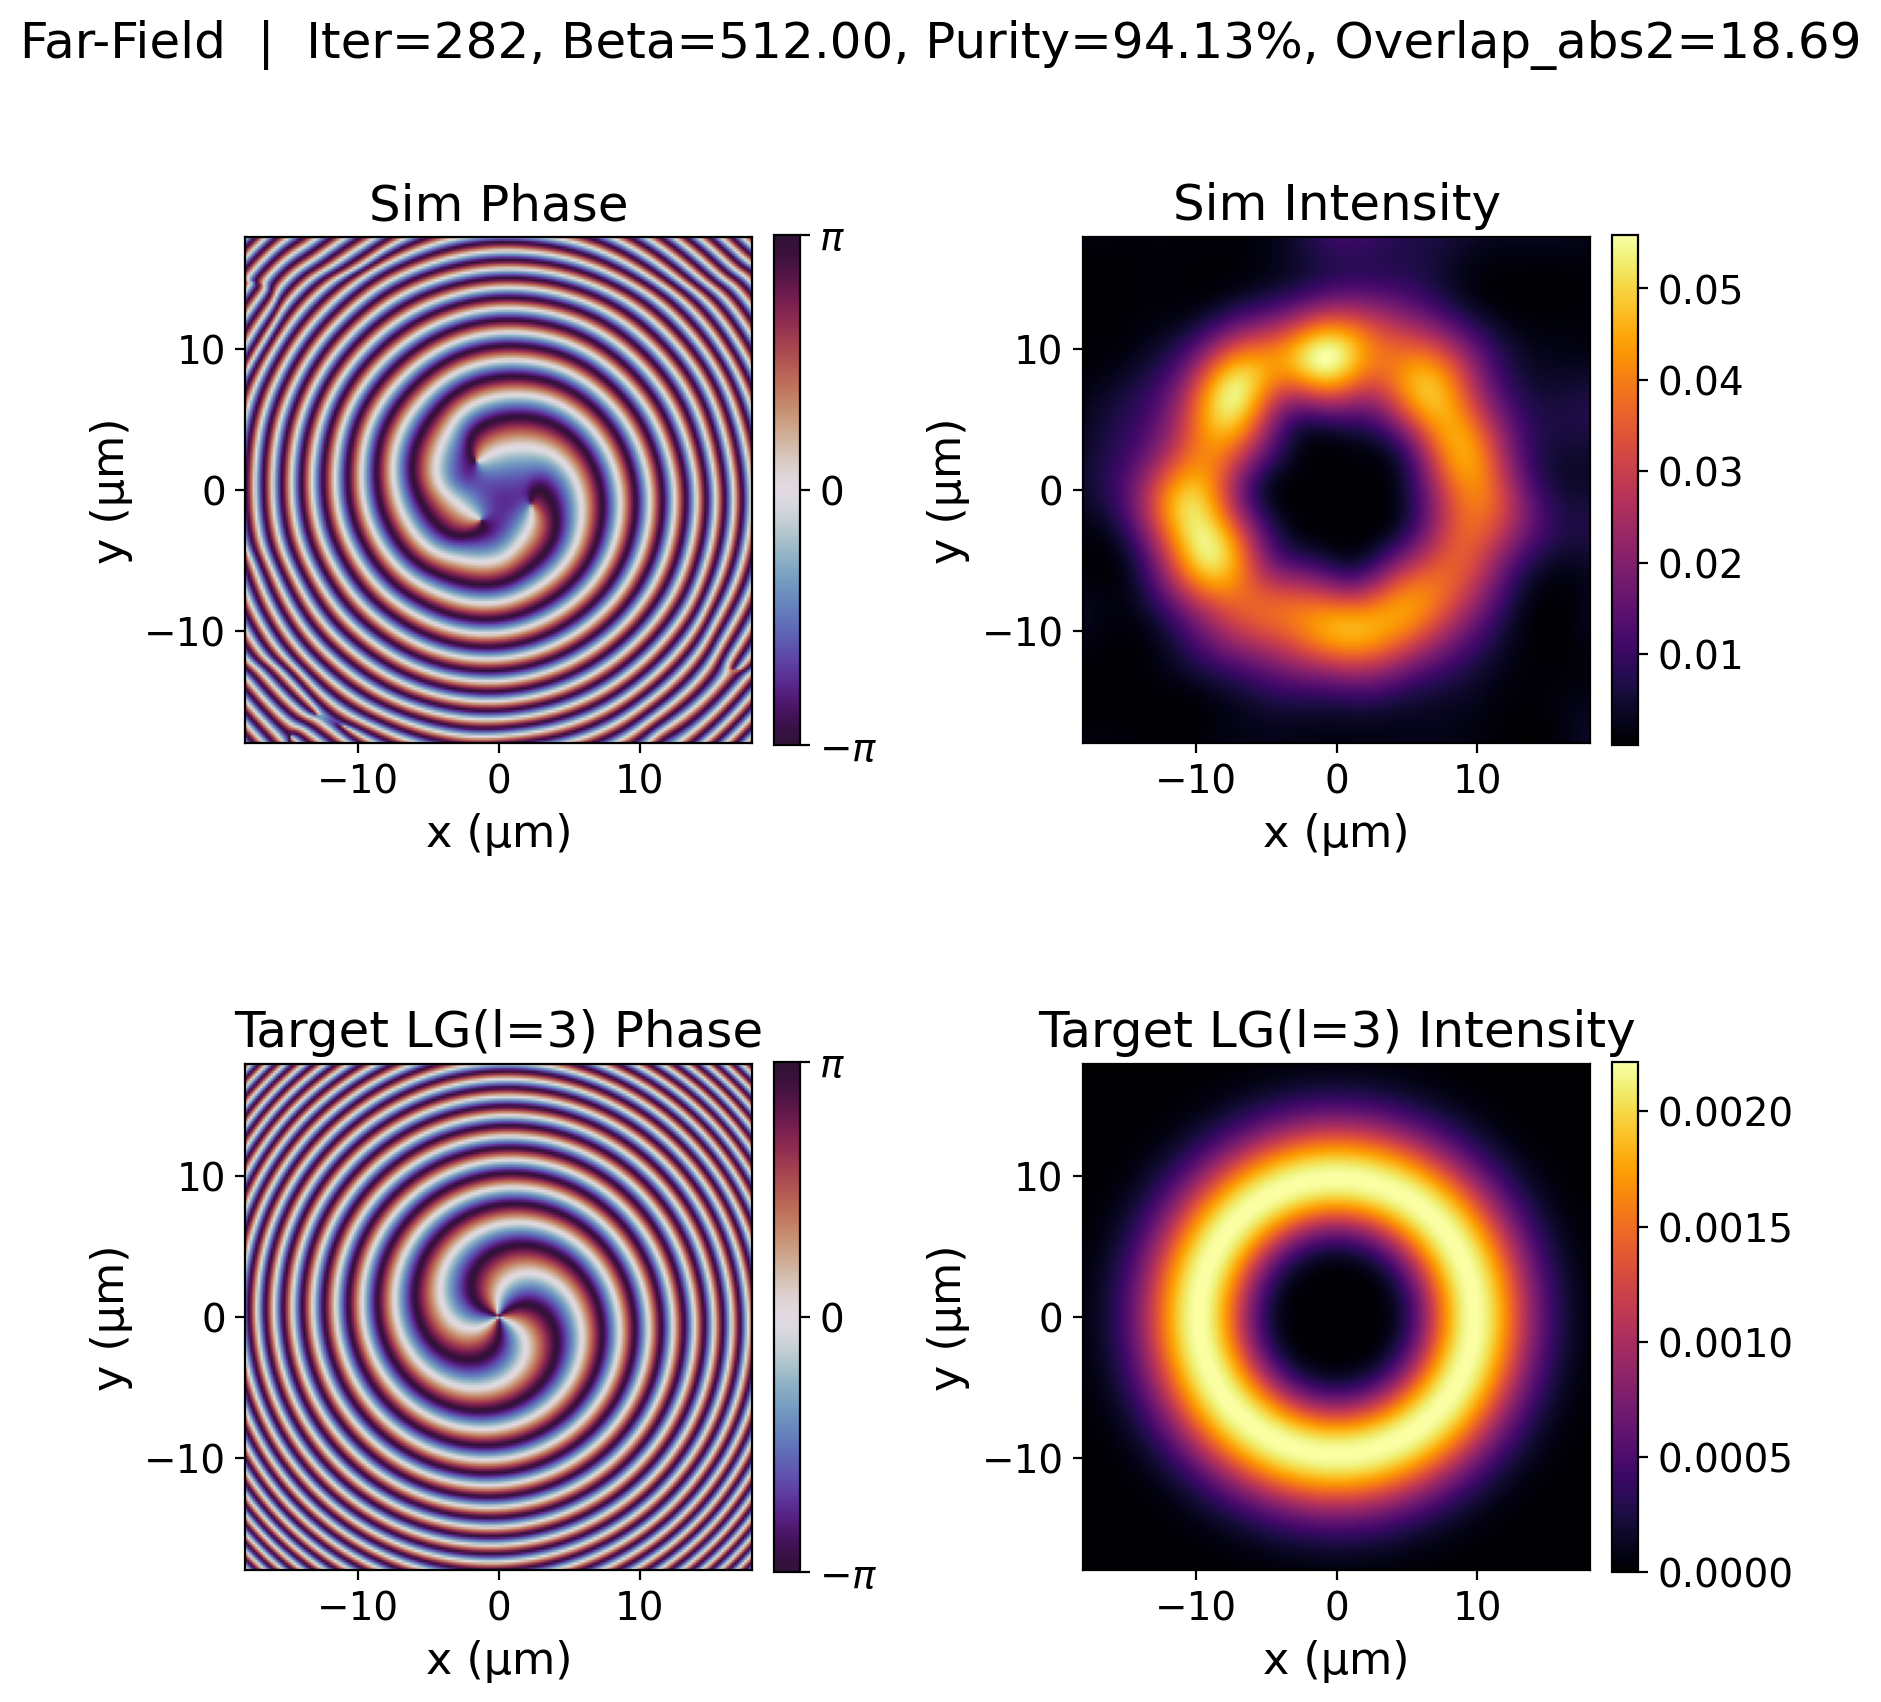
\includegraphics[width=0.23\textwidth,height=3.3cm,keepaspectratio]{img/020_ff_iter_282_beta_512.00.png} \\ {\small (a) $\ell=0$} & {\small (b) $\ell=1$} & {\small (c) $\ell=2$} & {\small (d) $\ell=3$} \\ 
\end{tabular}\\[6pt] 
\small\renewcommand{\arraystretch}{1.15} 
\begin{tabular}{ccccc} 
\toprule 
$\ell$ & Mode & Purity (\%) & $|\text{Ov}|^2$ & FOM \\
\midrule 
\rowcolor{accentgreen!20} 0 & $\text{LG}_{0,0}$ & 96.81 & 60.92 & 0.38 \\
\rowcolor{accentgreen!20} 1 & $\text{LG}_{1,0}$ & \textbf{98.66} & 53.88 & 0.39 \\
\rowcolor{accentgreen!20} 2 & $\text{LG}_{2,0}$ & 97.96 & 7.99 & 0.19 \\ 
\rowcolor{accentgreen!20} 3 & $\text{LG}_{3,0}$ & 94.13 & 18.69 & 0.23 \\
\bottomrule
\end{tabular}
{\small All four designs: purity $\ge94\%$ --- high LG mode fidelity}
\end{frame}

% [R-2] Far-Field: low-purity group

\begin{frame}{Far-Field LG Mode ($\ell=4,5$) at $z=10\,z_R$}
\begin{columns}[c]
\column{0.55\textwidth}
\centering
\begin{tabular}{cc}
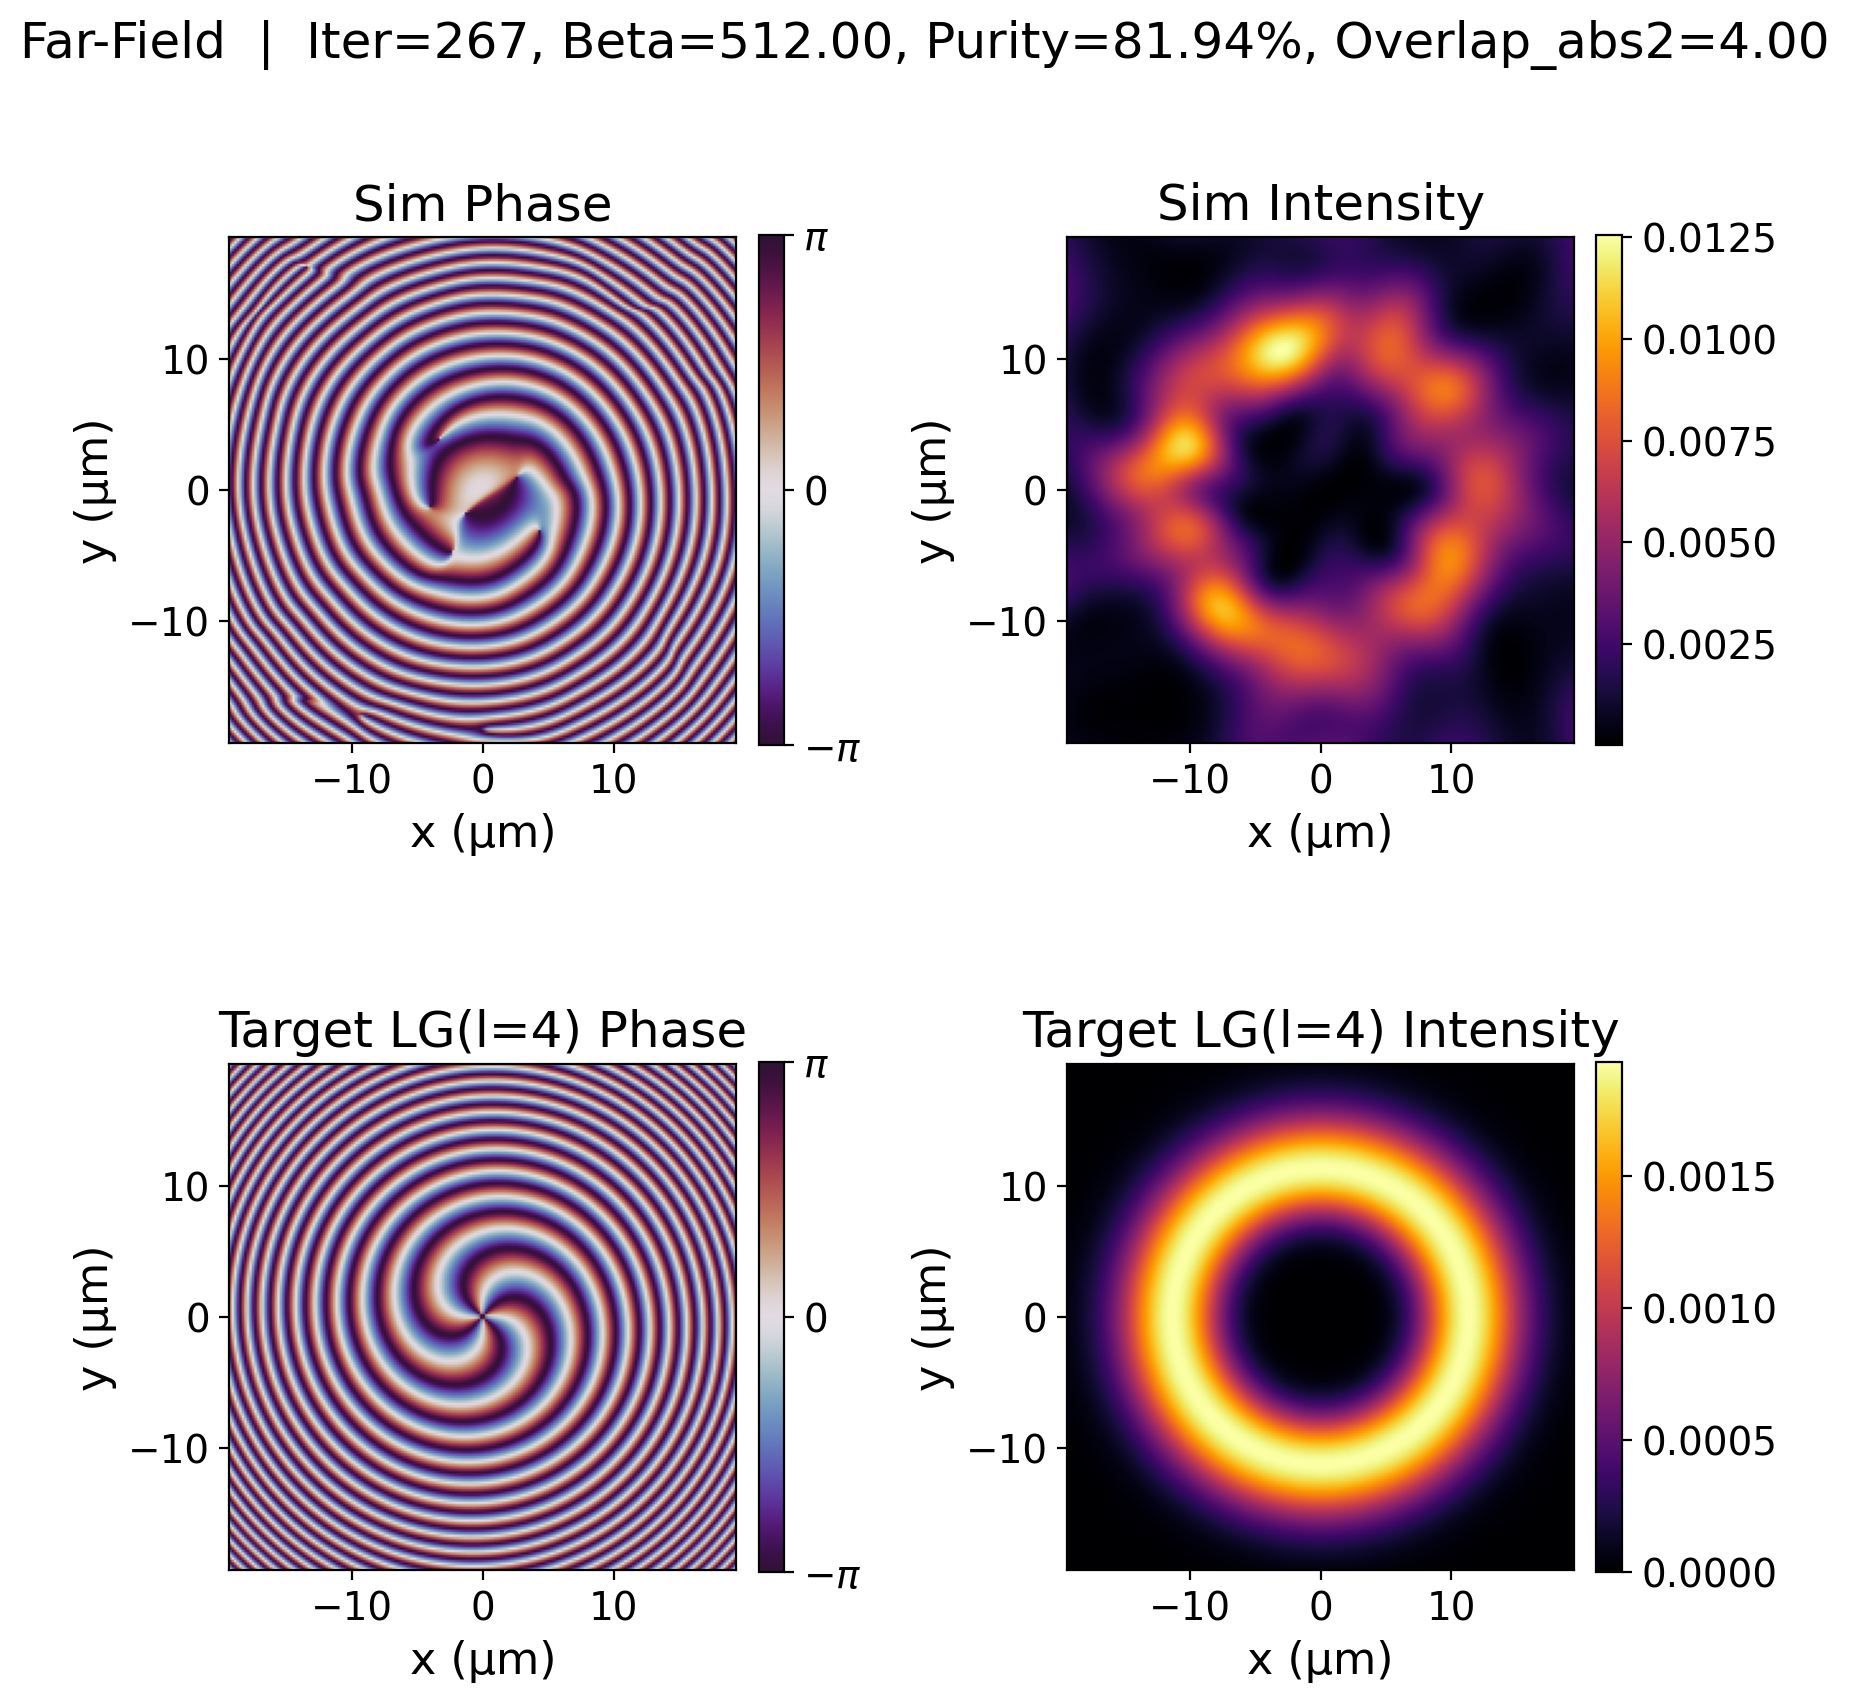
\includegraphics[width=0.46\columnwidth,height=3.0cm,keepaspectratio]{img/021_ff_iter_267_beta_512.00.png} &
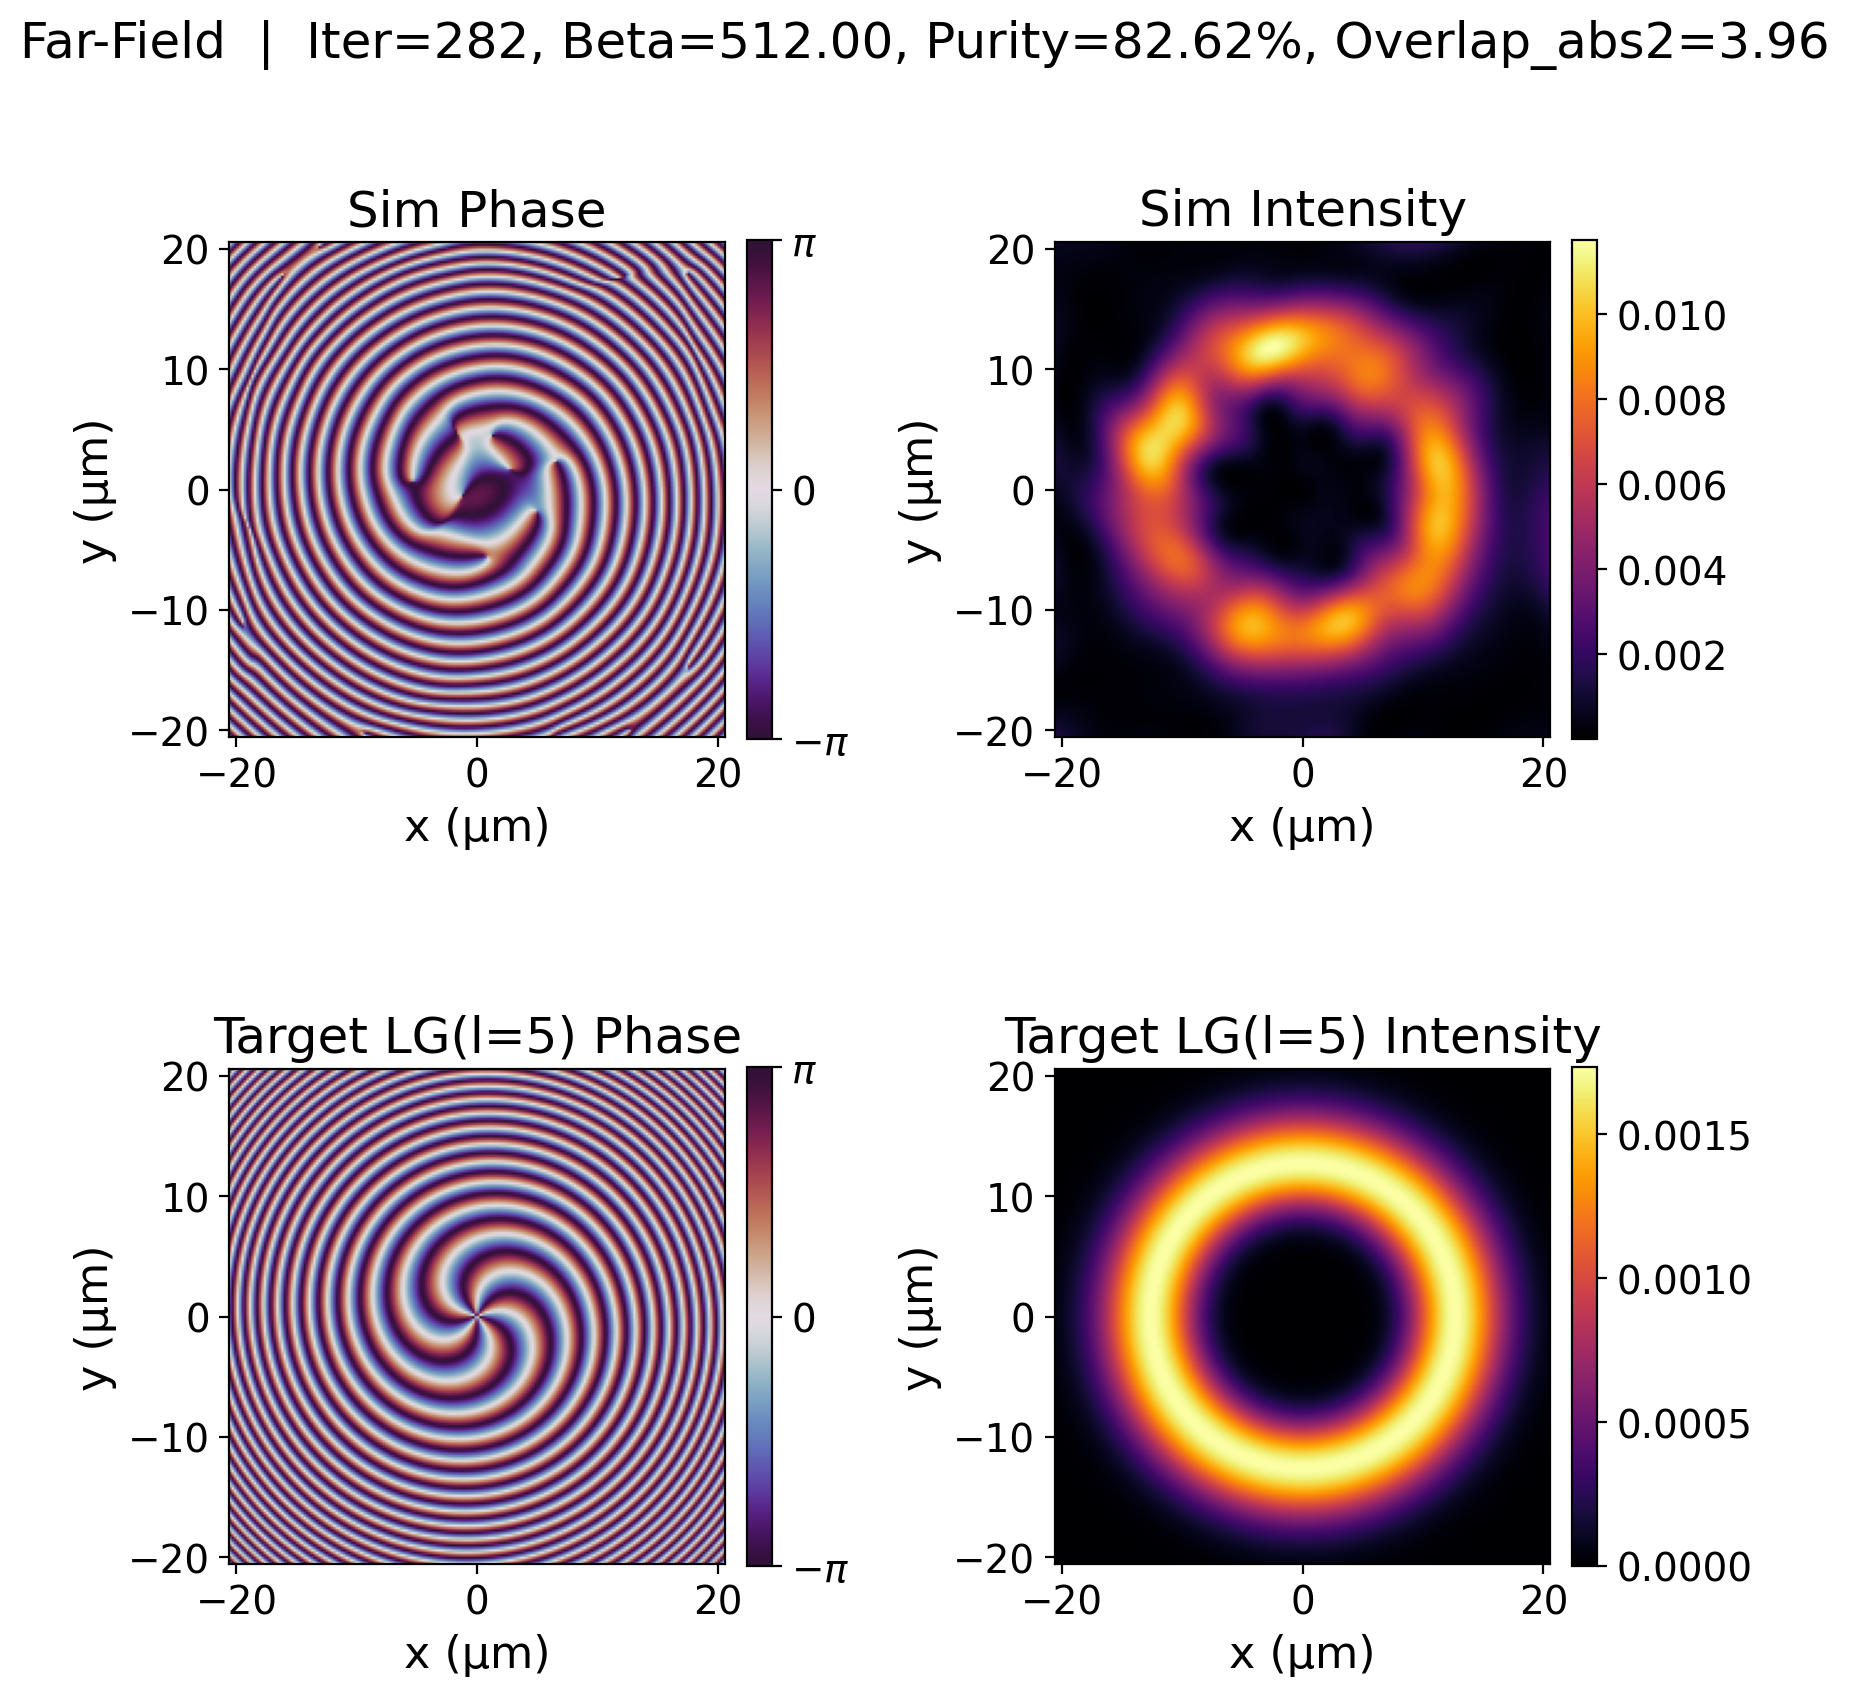
\includegraphics[width=0.46\columnwidth,height=3.0cm,keepaspectratio]{img/022_ff_iter_282_beta_512.00.png} \\
{\small (e) $\ell=4$} & {\small (f) $\ell=5$} \\
\end{tabular}\\[8pt]

\column{0.40\textwidth}
\centering
\small\renewcommand{\arraystretch}{1.15}
\begin{tabular}{ccccc}
\toprule
$\ell$ & Mode & Purity (\%) & $|\text{Ov}|^2$ & FOM \\
\midrule
\rowcolor{accentgreen!15} 0 & $\text{LG}_{0,0}$ & 96.81 & 60.92 & 0.38 \\
\rowcolor{accentgreen!15} 1 & $\text{LG}_{1,0}$ & \textbf{98.66} & 53.88 & 0.39 \\
\rowcolor{accentgreen!15} 2 & $\text{LG}_{2,0}$ & 97.96 & 7.99  & 0.19 \\
\rowcolor{accentgreen!15} 3 & $\text{LG}_{3,0}$ & 94.13 & 18.69 & 0.23 \\
\rowcolor{NYCUgold!25}  4 & $\text{LG}_{4,0}$ & 81.94 & 4.00  & -0.06 \\
\rowcolor{NYCUgold!25}  5 & $\text{LG}_{5,0}$ & 82.62 & 3.96  & -0.05 \\
\bottomrule
\end{tabular}\\[6pt]

{\small Constrained by design area degrees of freedom, purity drops to $\sim 82\%$.}
\end{columns}
\end{frame}


% [R-6] Phase Winding

\begin{frame}{Phase Winding: Topological Charge Accuracy}
  \begin{columns}[T]
    \column{0.60\textwidth}
      \centering
      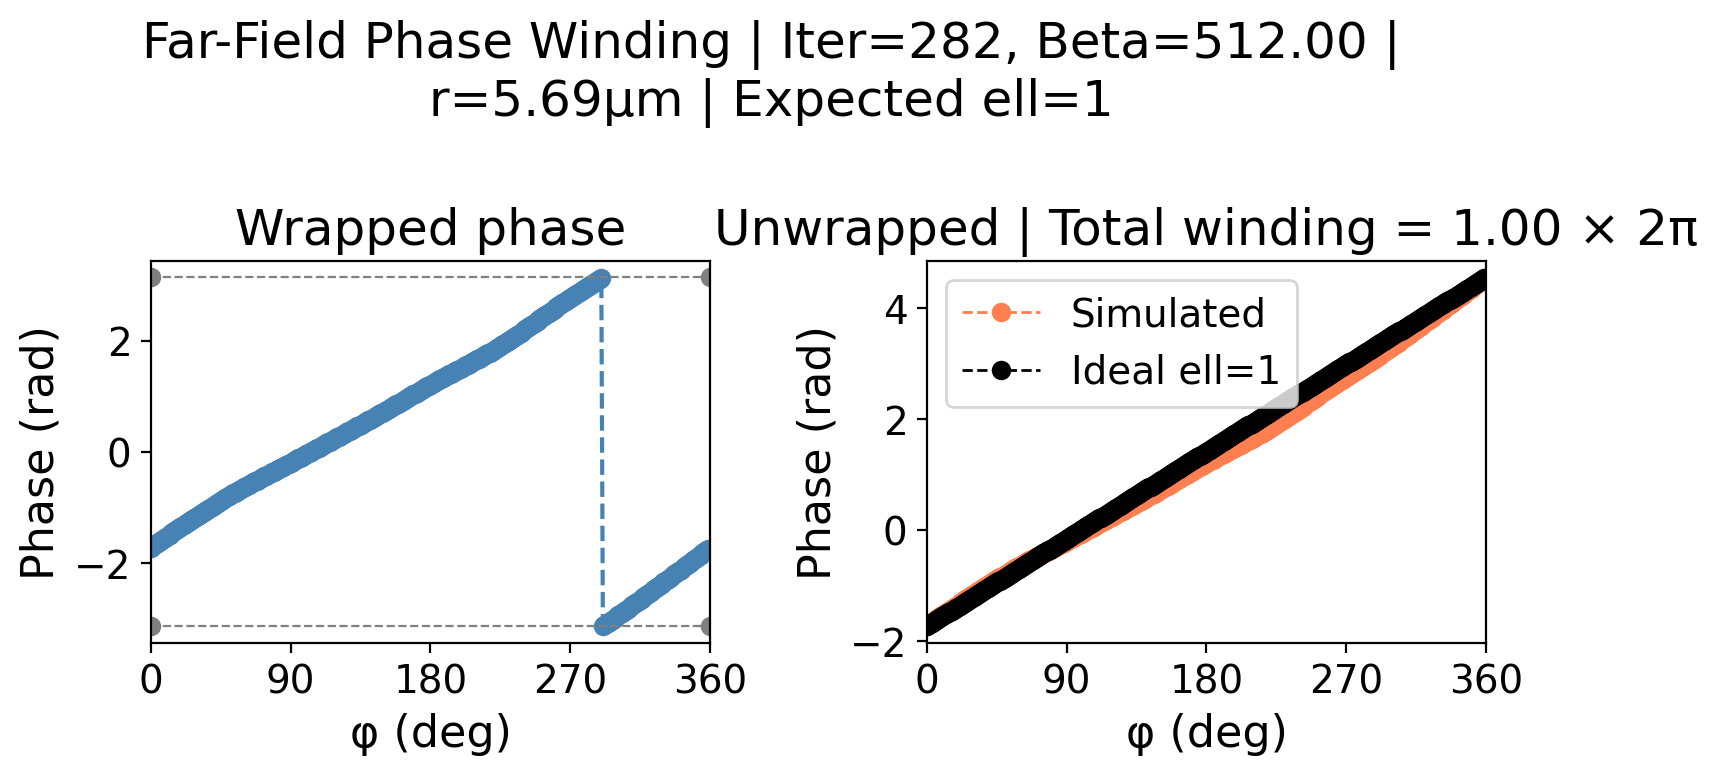
\includegraphics[width=\textwidth,height=3.5cm,keepaspectratio]{img/018_ff_winding_iter_282_beta_512.00_rfraction_0.3885.png}\\
      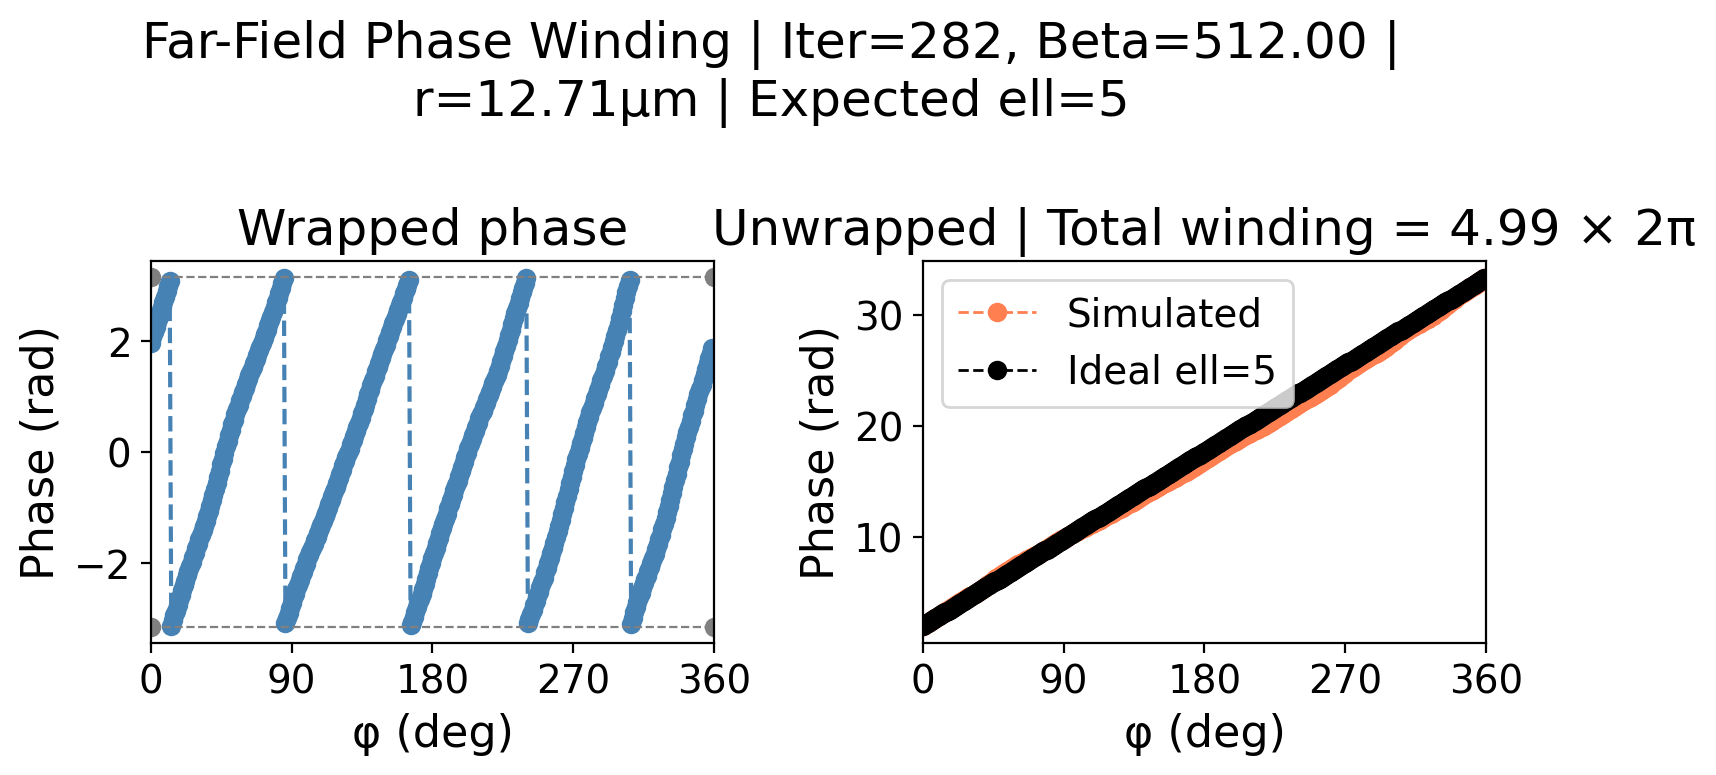
\includegraphics[width=\textwidth,height=3.5cm,keepaspectratio]{img/022_ff_winding_iter_282_beta_512.00_rfraction_0.6176.png}
	  \column{0.37\textwidth}
	  \centering
	  \vspace{1cm}
	  \begin{exampleblock}{All Six Designs}
		\small\centering
		\begin{tabular}{lr}
		  \toprule
		  $\ell$ & Error \\
		  \midrule
		  0 & $\approx0$ \\
		  1 & $<0.1\%$ \\
		  2 & $0.5\%$ \\
		  3 & $<1\%$ \\
		  4 & $<1\%$ \\
		  5 & $<1\%$ \\
		  \bottomrule
		\end{tabular}
	  \end{exampleblock}
  \end{columns}
\end{frame}

  

% [R-7] Chirality

\begin{frame}{Chirality Propagation}
  \begin{columns}[T]
    \column{0.7\textwidth}
      \centering
      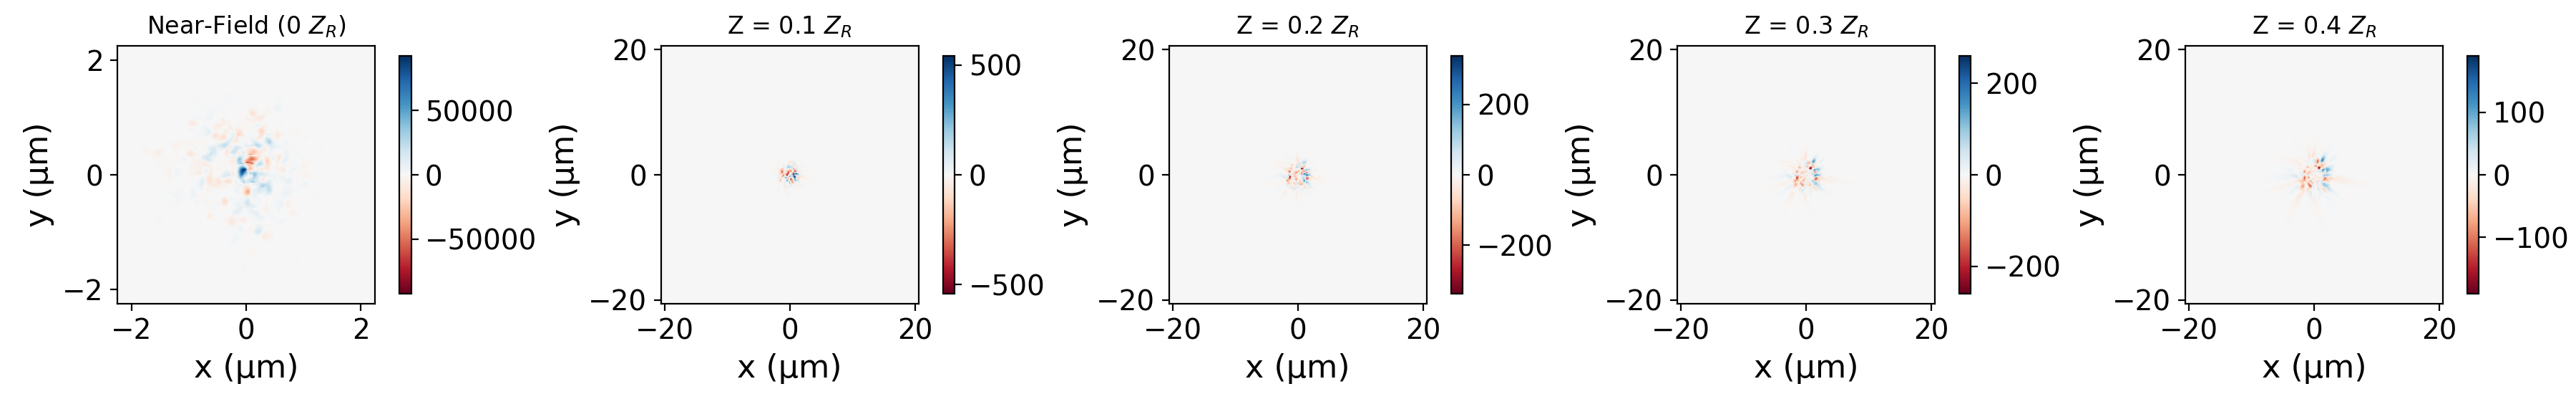
\includegraphics[width=\textwidth,height=2.1cm,keepaspectratio]{img/chirality_prop_0p0to0p9zr_Fixed_XY_360_1.png}\\[1pt]
      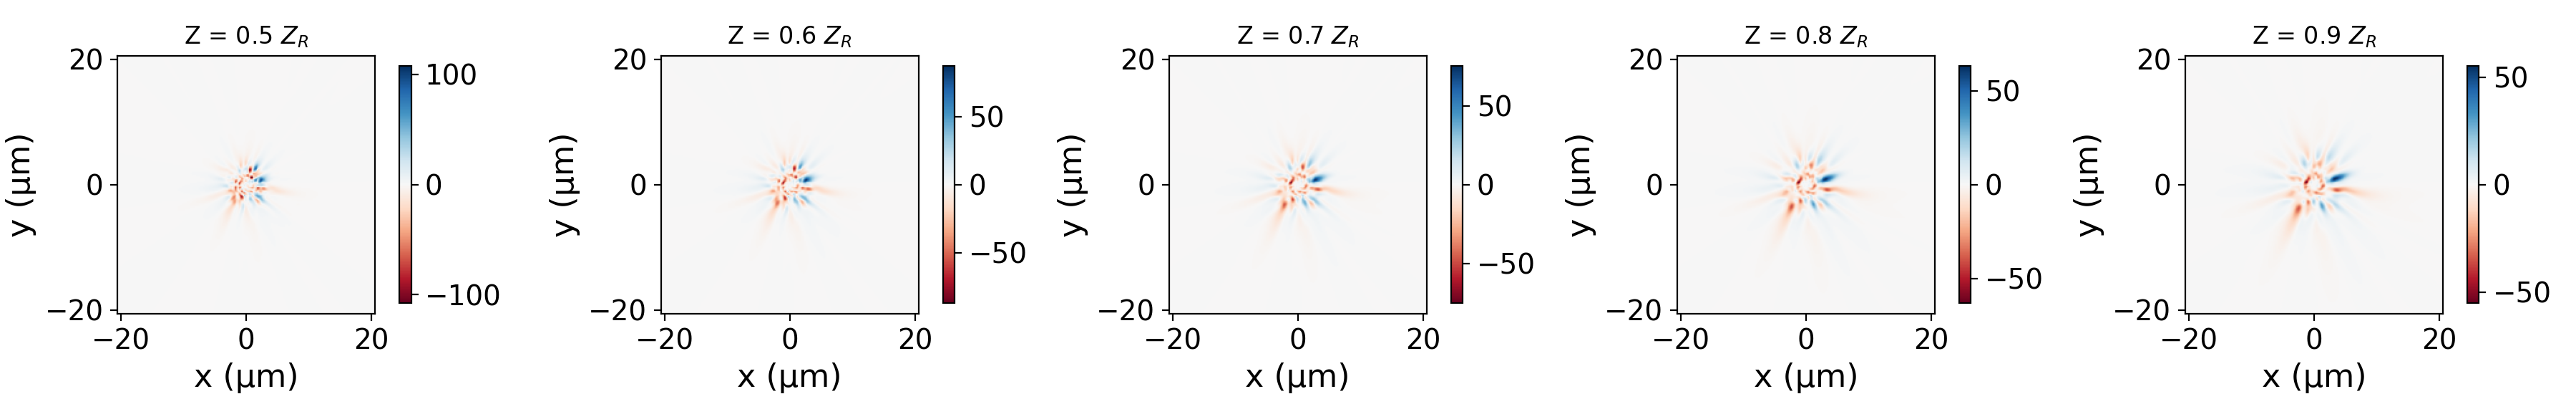
\includegraphics[width=\textwidth,height=2.1cm,keepaspectratio]{img/chirality_prop_0p0to0p9zr_Fixed_XY_360_2.png}\\[1pt]
      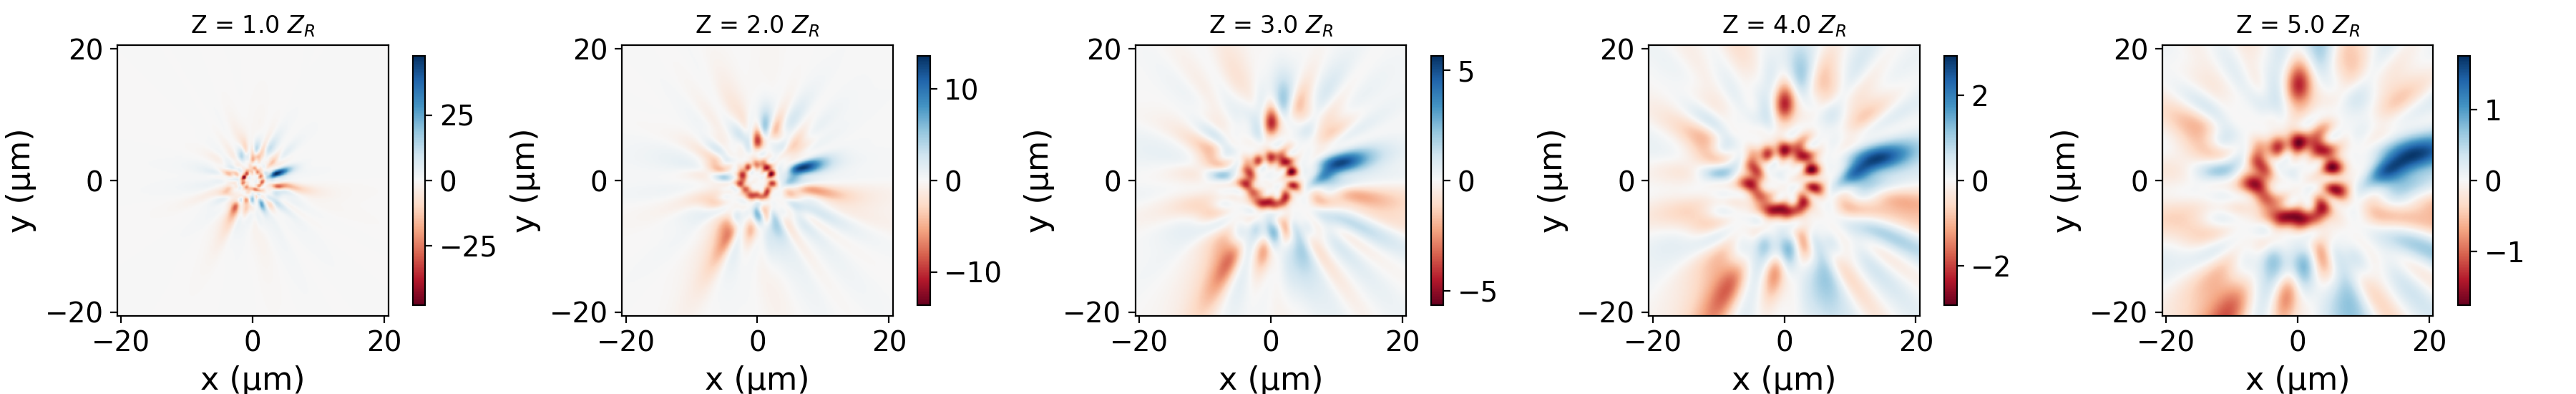
\includegraphics[width=\textwidth,height=2.1cm,keepaspectratio]{img/chirality_prop_1to10zr_Fixed_XY_360_1.png}\\[1pt]
      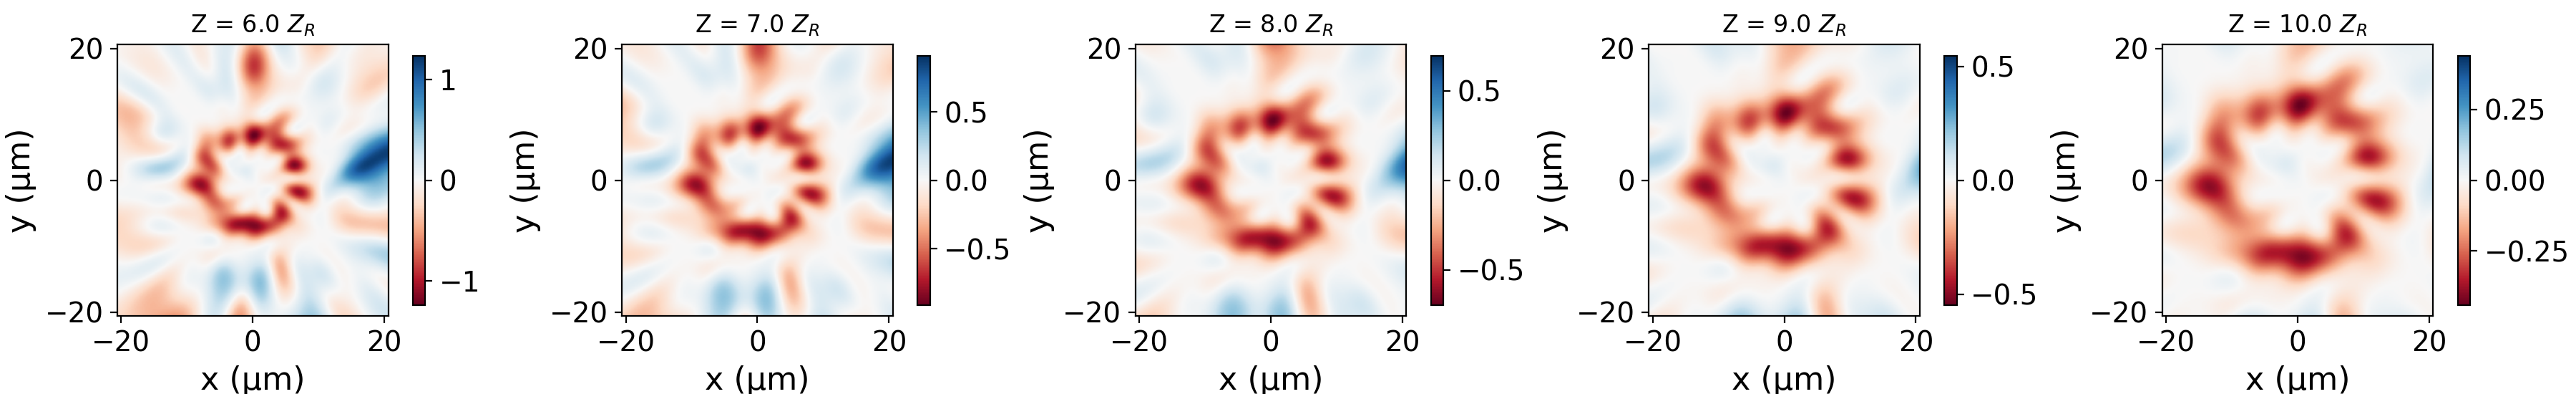
\includegraphics[width=\textwidth,height=2.1cm,keepaspectratio]{img/chirality_prop_1to10zr_Fixed_XY_360_2.png}
    \column{0.30\textwidth}
    \vspace{2cm}
    {\large \textbf{Chirality}: }\\[4pt]
    {$C=\pi f\,\mathrm{Im}(\mathbf{E}^*\cdot\mathbf{H})$}\\[12pt]
    \textbf{\textcolor{red}{Red ($C<0$): LCP}}\\[6pt]
    \textbf{\textcolor{blue}{Blue ($C>0$): RCP}}
  \end{columns}
\end{frame}

  

% [R-8] Valley Selectivity -- "Physical Origin" block filled (Results
% section, kept detailed per instruction). Grounded in the D3h selection
% rules already used in Backup: Valley Selection Rule.

\begin{frame}{Valley Selectivity: Cross-Polarization Test}
  \begin{columns}[T]
    \column{0.48\textwidth}
      \centering
      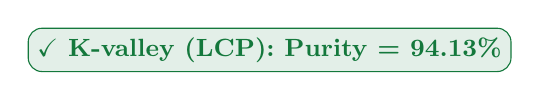
\begin{tikzpicture}
        \node[draw=accentgreen,fill=accentgreen!12,rounded corners=5pt,minimum width=5.5cm,minimum height=0.5cm,font=\small\bfseries]{\grn{\checkmark\ K-valley (LCP): Purity = 94.13\%}};
      \end{tikzpicture}\\[1pt]
      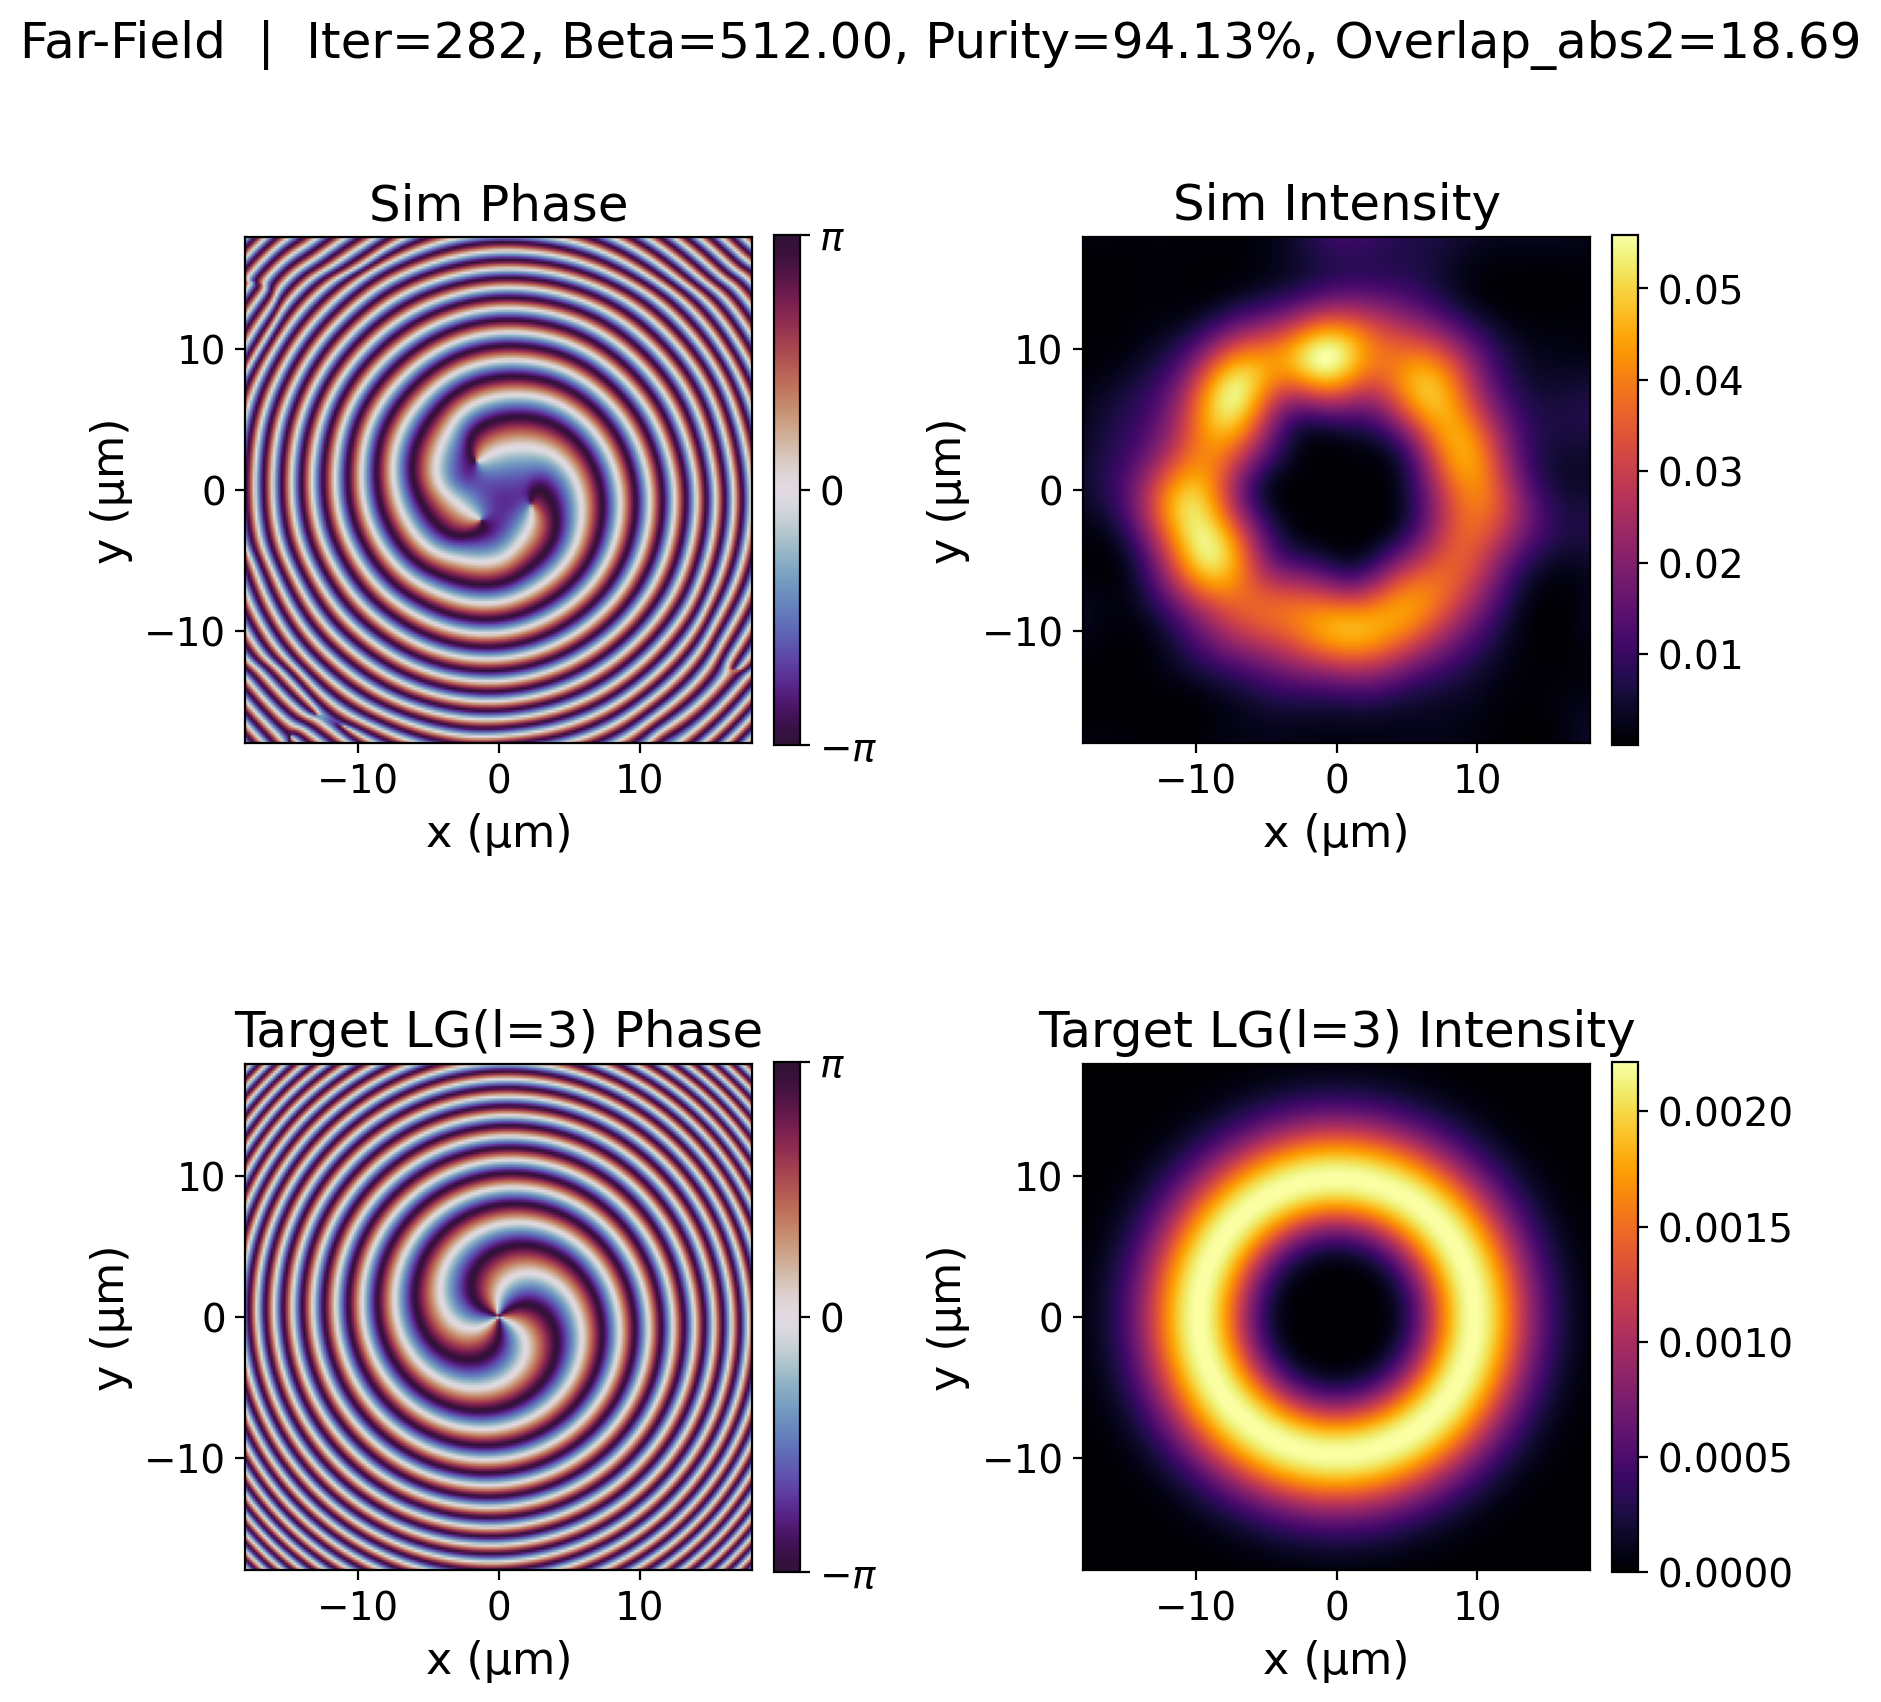
\includegraphics[width=1\textwidth,height=5.5cm,keepaspectratio]{img/020_ff_iter_282_beta_512.00.png}\\
    \column{0.48\textwidth}
      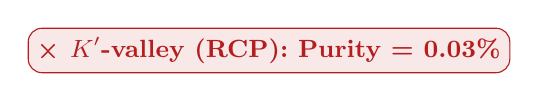
\begin{tikzpicture}
        \node[draw=accentred,fill=accentred!10,rounded corners=5pt,minimum width=5.5cm,minimum height=0.5cm,font=\small\bfseries]{\red{\texttimes\ $K'$-valley (RCP): Purity = 0.03\%}};
      \end{tikzpicture}\\[1pt]
      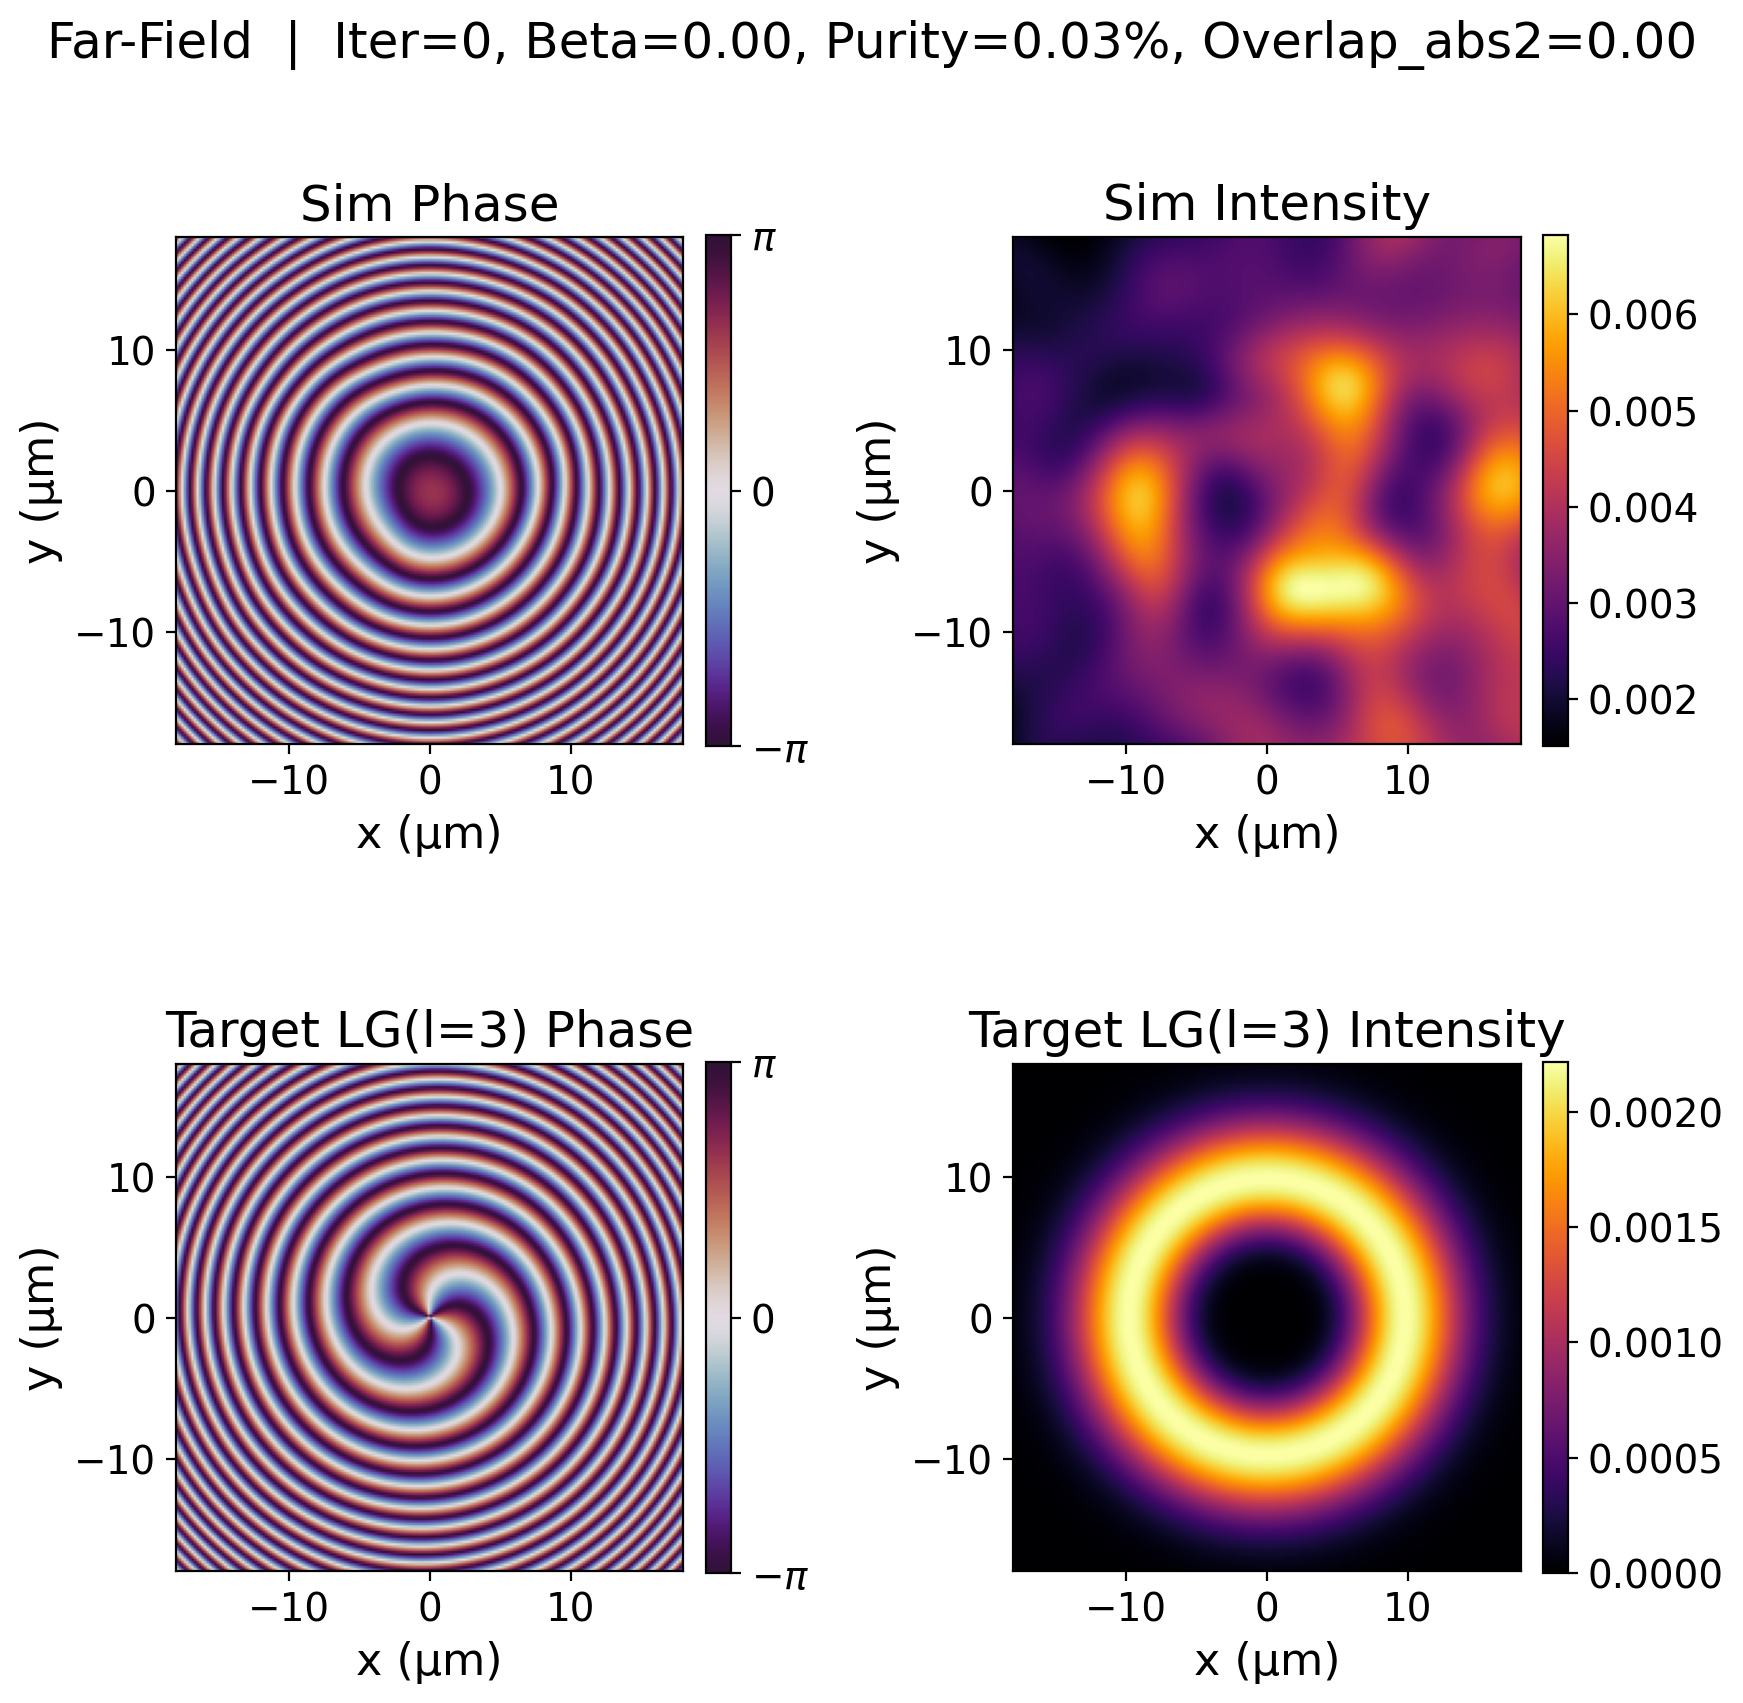
\includegraphics[width=1\textwidth,height=5.5cm,keepaspectratio]{img/rcp.png}\\
\end{columns}
\vspace{0.3cm}
\begin{center}
{\small Valley Contrast Ratio: \textcolor{NYCUblue}{$\approx \textbf{3143: 1}$}}
\end{center}
\end{frame}

% [R-4.5] Device Physical Conversion Efficiency -- NEW FRAME (student request)
% VERIFY: numbers below are for ell=5 only (purity 82.62% matches the
% ell=5 far-field result on R-4/R-5). Confirm whether this frame should
% represent (a) ell=5 as the worst-case/representative example, or
% (b) all six designs as a summary table -- currently drafted as (a).

\begin{frame}{Device Energy Efficiency}
\begin{columns}[T]
\begin{column}{0.46\textwidth}
\centering
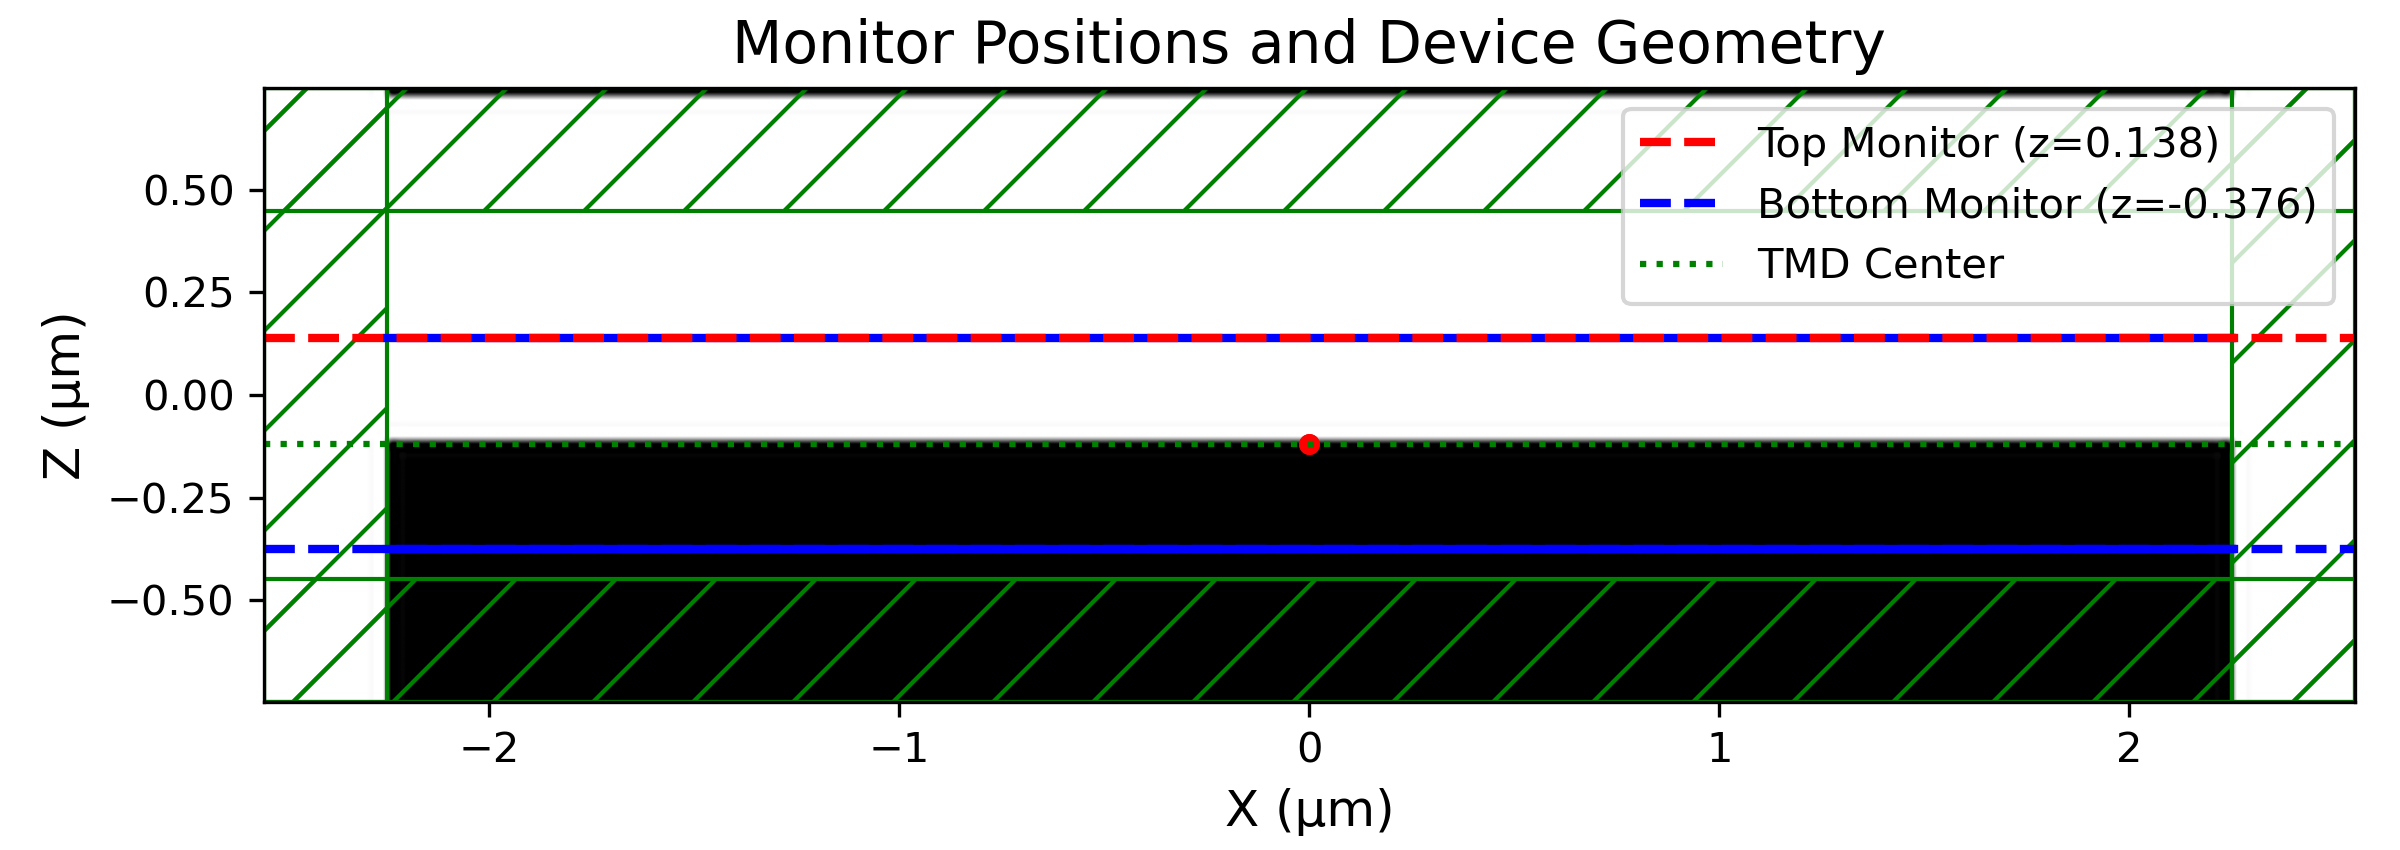
\includegraphics[width=\linewidth,height=3.3cm,keepaspectratio]{img/monitor_positions_air.png}\\[4pt]
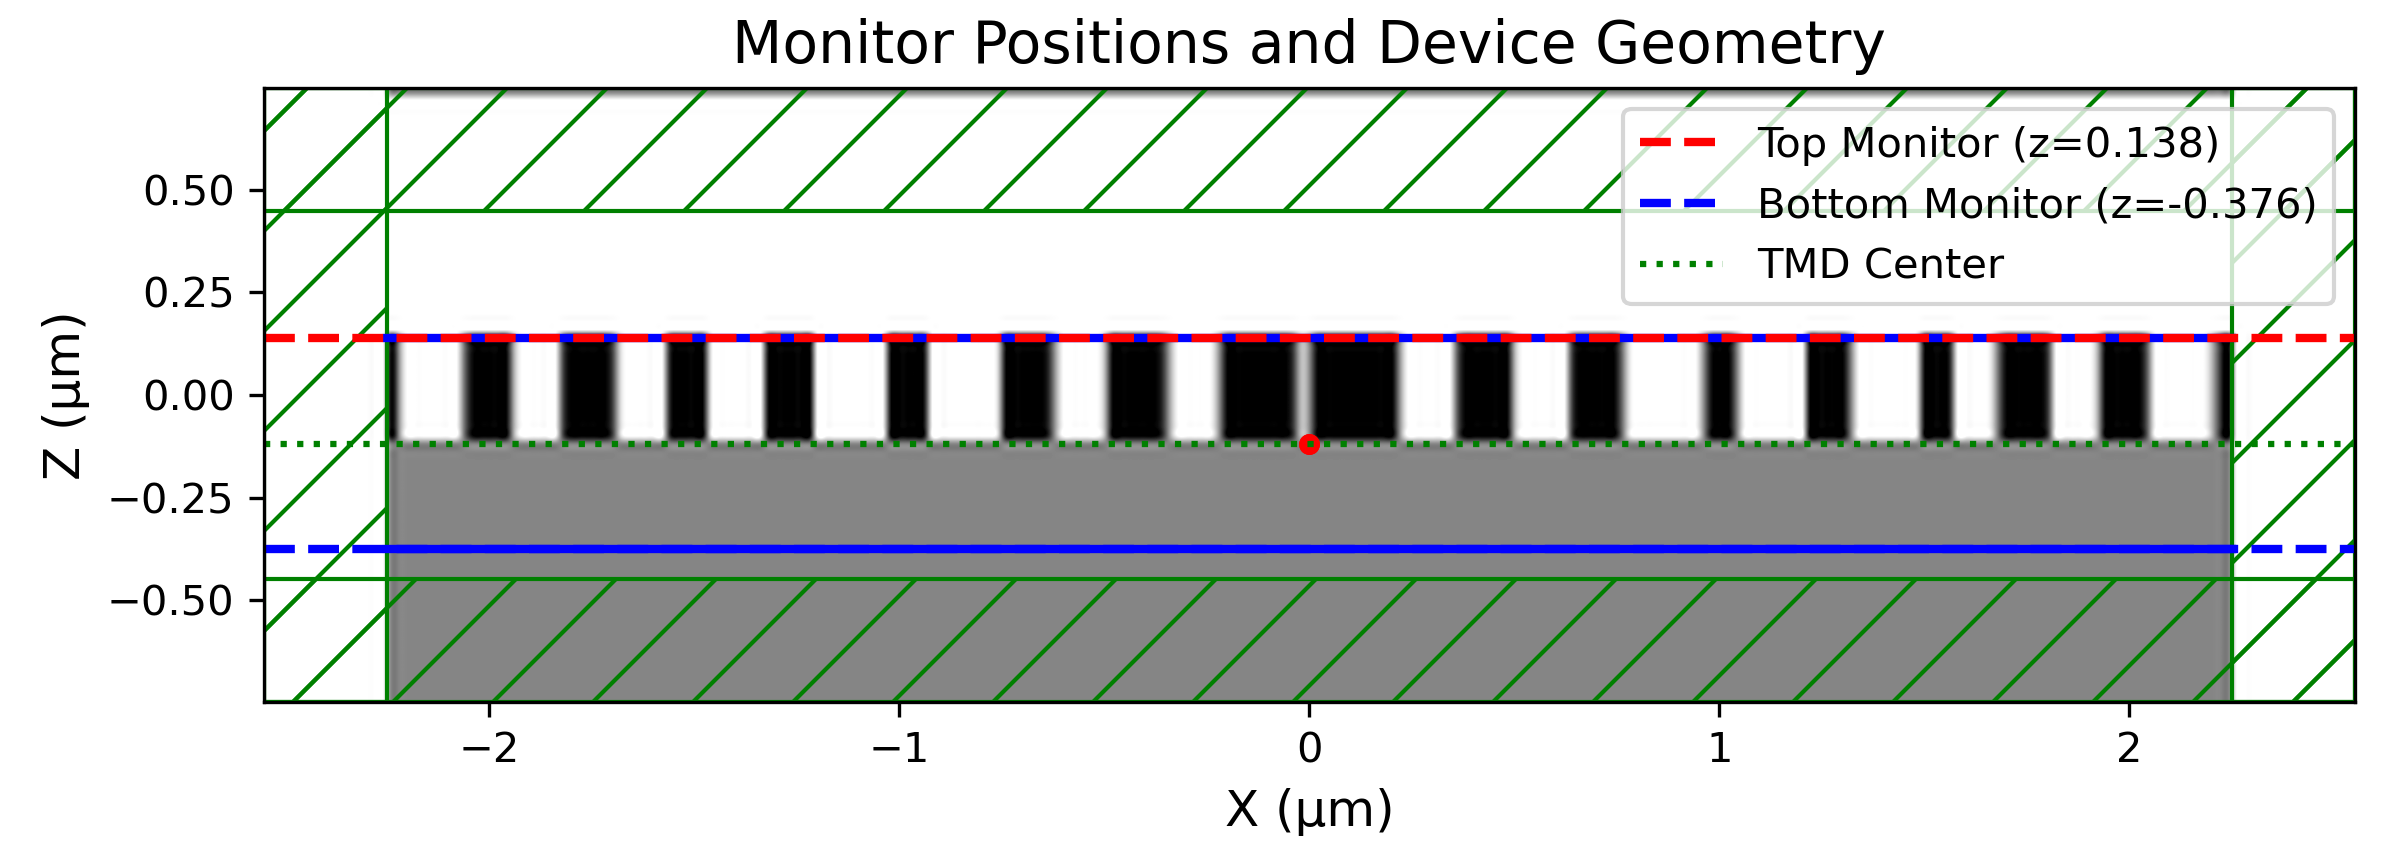
\includegraphics[width=\linewidth,height=3.3cm,keepaspectratio]{img/monitor_positions_ell2.png}
\end{column}
\begin{column}{0.54\textwidth}
\begin{block}{Efficiency Evaluation}
\scriptsize
\begin{itemize}
    \item $X$ (Upward Fraction): $X = (P_{\text{up}} / P_{\text{total}}) \times 100\%$
    \item $Y$ (Far-Field Purity): Measured modal purity (\%)
    \item $Z$ (Device Efficiency): $Z = X \times Y$
\end{itemize}
\centering
\end{block}
\resizebox{\linewidth}{!}{%
\begin{tabular}{cccccc}
\toprule
Structure & $P_{\text{up}}$ (W) & $P_{\text{total}}$ (W) & X (\%) & Y (\%) & Z (\%) \\
\midrule
 Pure Air & $5.0 \times 10^1$ & $1.0 \times 10^3$ & 5.04  & 100.00 & 5.04  \\
\rowcolor{accentgreen!20} $\ell = 0$          & $1.6 \times 10^2$ & $9.2 \times 10^2$ & 17.67 & 96.81  & 17.11 \\
\rowcolor{accentgreen!20} $\ell = 1$          & $9.2 \times 10^1$ & $9.5 \times 10^2$ & 9.67  & 98.66  & 9.54  \\
\rowcolor{accentgreen!20} $\ell = 2$          & $3.5 \times 10^1$ & $1.2 \times 10^3$ & 2.93  & 96.76  & 2.84  \\
\rowcolor{accentgreen!20} $\ell = 3$          & $6.3 \times 10^1$ & $1.5 \times 10^3$ & 4.22  & 94.13  & 3.97  \\
\rowcolor{NYCUgold!25} $\ell = 4$          & $3.5 \times 10^1$ & $1.2 \times 10^3$ & 2.93  & 81.94  & 2.40  \\
\rowcolor{NYCUgold!25} $\ell = 5$          & $2.4 \times 10^1$ & $1.1 \times 10^3$ & 2.14  & 82.62  & 1.77  \\
\bottomrule
\end{tabular}% 
}
\end{column}
\end{columns}
\centering
\vspace{0.5cm}
{\small Overall efficiency (Z) is bottlenecked by upward extraction (X), not modal purity (Y).}
\end{frame}


% [R-10] Comparison

\begin{frame}{Comparison with Prior Work}

  \centering\small\renewcommand{\arraystretch}{1.25}

\begin{columns}[T]
    \column{0.32\textwidth}
      \begin{exampleblock}{\centering Advantage (i)}
        \centering\footnotesize \textbf{Active source} + high LG purity ($>$94\% for $\ell\le3$) simultaneously
      \end{exampleblock}
    \column{0.32\textwidth}
      \begin{exampleblock}{\centering Advantage (ii)}
        \centering\footnotesize \textbf{Quantified} valley contrast: RCP 0.03\% vs.\ LCP 94.13\%
      \end{exampleblock}
    \column{0.32\textwidth}
      \begin{exampleblock}{\centering Advantage (iii)}
        \centering\footnotesize \textbf{Compact footprint:} $20.25 \mu m^2$ PIC-compatible
      \end{exampleblock}
  \end{columns}
  \vspace{4pt}
  \begin{tabular}{lccccc}
    \toprule
    \textbf{Work} & \textbf{Design} & Footprint & \textbf{Purity} & \textbf{Source} & \textbf{Valley sel.} \\
    \midrule
    Karimi 2014 & Forward (PB)      & $9 \times 10^2 \mu m^2$ & $\sim$64\%  & Passive PW & \red{None} \\
    Sroor 2020  & Forward, $\text{TiO}_2$  & $4 \times 10^4 \mu m^2$ & $\sim90\%$ ($\ell\!\le\!100$) & Intracavity & \red{None} \\
    Rong 2023 & Rashba Kagome BIC & $3.28 \times 10^2 \mu m^2$ & Not quantified & Active ($\text{WS}_2$) & Valley coherent \\
    Li 2023     & BIC photonic crystal & $2.89 \times 10^2 \mu m^2$ & Not quantified & Active ($\text{WSe}_2$) & Fixed $\ell$ \\
    \midrule
    \rowcolor{NYCUblue!15}
    \textbf{This work} & \textbf{Inverse (topo.\ opt.)} & $20.25 \mu m^2$ & \textbf{82--98\%} & \textbf{Active $\text{WS}_2$} & \makecell{\textbf{Valley coherent} \\ \textcolor{green!60!black}{\textbf{$>$1000:1}}} \\
    \bottomrule
  \end{tabular}
\end{frame}



\section{Conclusions \& Future Work}



% [DIVIDER-4]
\begin{frame}[plain]

  \begin{tikzpicture}[remember picture,overlay]
    \fill[NYCUblue](current page.south west) rectangle (current page.north east);
    \node[white,font=\Huge\bfseries] at (current page.center){4.\ Conclusions \& Future Work};
  \end{tikzpicture}
\end{frame}



% [C-1] Conclusions -- kept as full sentences (exception to keyword rule),
% UNCHANGED per instruction.

\begin{frame}{Conclusions}
  \begin{enumerate}
    \setlength\itemsep{7pt}
    \item \textbf{High-purity OAM from an active valley source}\\
      Purity $\ge94\%$ for $\ell\le3$; peak \highlight{98.66\%} at $\ell=1$; phase winding error $<1\%$ for all six designs.
    \item \textbf{Topology-driven structural diversity} \\ 
    $\ell=2$ uniquely forms a two-arm SPP-like spiral, while other designs exhibit non-intuitive free-form geometries.\\
    \item \textbf{Strong valley selectivity}\\
      K-valley (LCP) 94.13\% vs.\ K'-valley (RCP) 0.03\% (ratio $>1000:1$).
    \item \textbf{Chirality Propagation}\\
      Mixed LCP/RCP near field $\to$ pure LCP far field as evanescent waves decay. OAM reshaping and SAM decoupled.
      \item \textbf{Device energy efficiency}\\
	  Device efficiency peaks at \highlight{17.11\%} ($\ell=0$, $3.4\times$ pure air) and 9.54\% ($\ell=1$); efficiency is bottlenecked by upward extraction, not purity.
  \end{enumerate}
\end{frame}

 

% [C-2] Future Work -- block (iii) filled. "Substracts" in your draft was
% assumed to be a typo for "Substrates"; VERIFY and edit if you meant
% something else (e.g. fabrication tolerance study specifically).

\begin{frame}{Future Work}
  \begin{columns}[T]
    \column{0.8\textwidth}
      \begin{block}{(i) Expand Design Domain}
        Target $\ge6.5\,\mu$m + higher resolution\\
        Expected: purity $>85\%$ for $\ell=4,5$
      \end{block}
      \vspace{1pt}
	\begin{block}{(ii) Complete Topological-Charge Coverage ($\ell \in [-5, 5]$)} 
		Expanded Simulation Scope: Include negative OAM modes ($\ell = -1 \text{ to } -5$).
	\end{block}
      \vspace{1pt}
      \begin{block}{(iii) Alternative Substrates}
        lower-index substrate, e.g.\ $\text{MgF}_2$ ($n\approx1.38$) $\Rightarrow$ higher device energy efficiency
      \end{block}
  \end{columns}
\end{frame}

  

% [THANK-YOU]

\begin{frame}[plain]
  \vspace{0.5cm}
  \begin{center}
    {\large\textcolor{darkgray}{Q \& A}}\\[0.7cm]
    {\color{NYCUblue}\rule{10cm}{1.5pt}}\\[0.5cm]
    {\normalsize \textbf{Yin-Jie Cheng}\quad|\quad Advisor: Prof.\ Jhih-Sheng Wu\\[4pt] Department of Photonics, NYCU\quad|\quad August 2026}\\[0.5cm]
  \end{center}
  \begin{columns}[c]
    \column{0.30\textwidth}
      \centering
      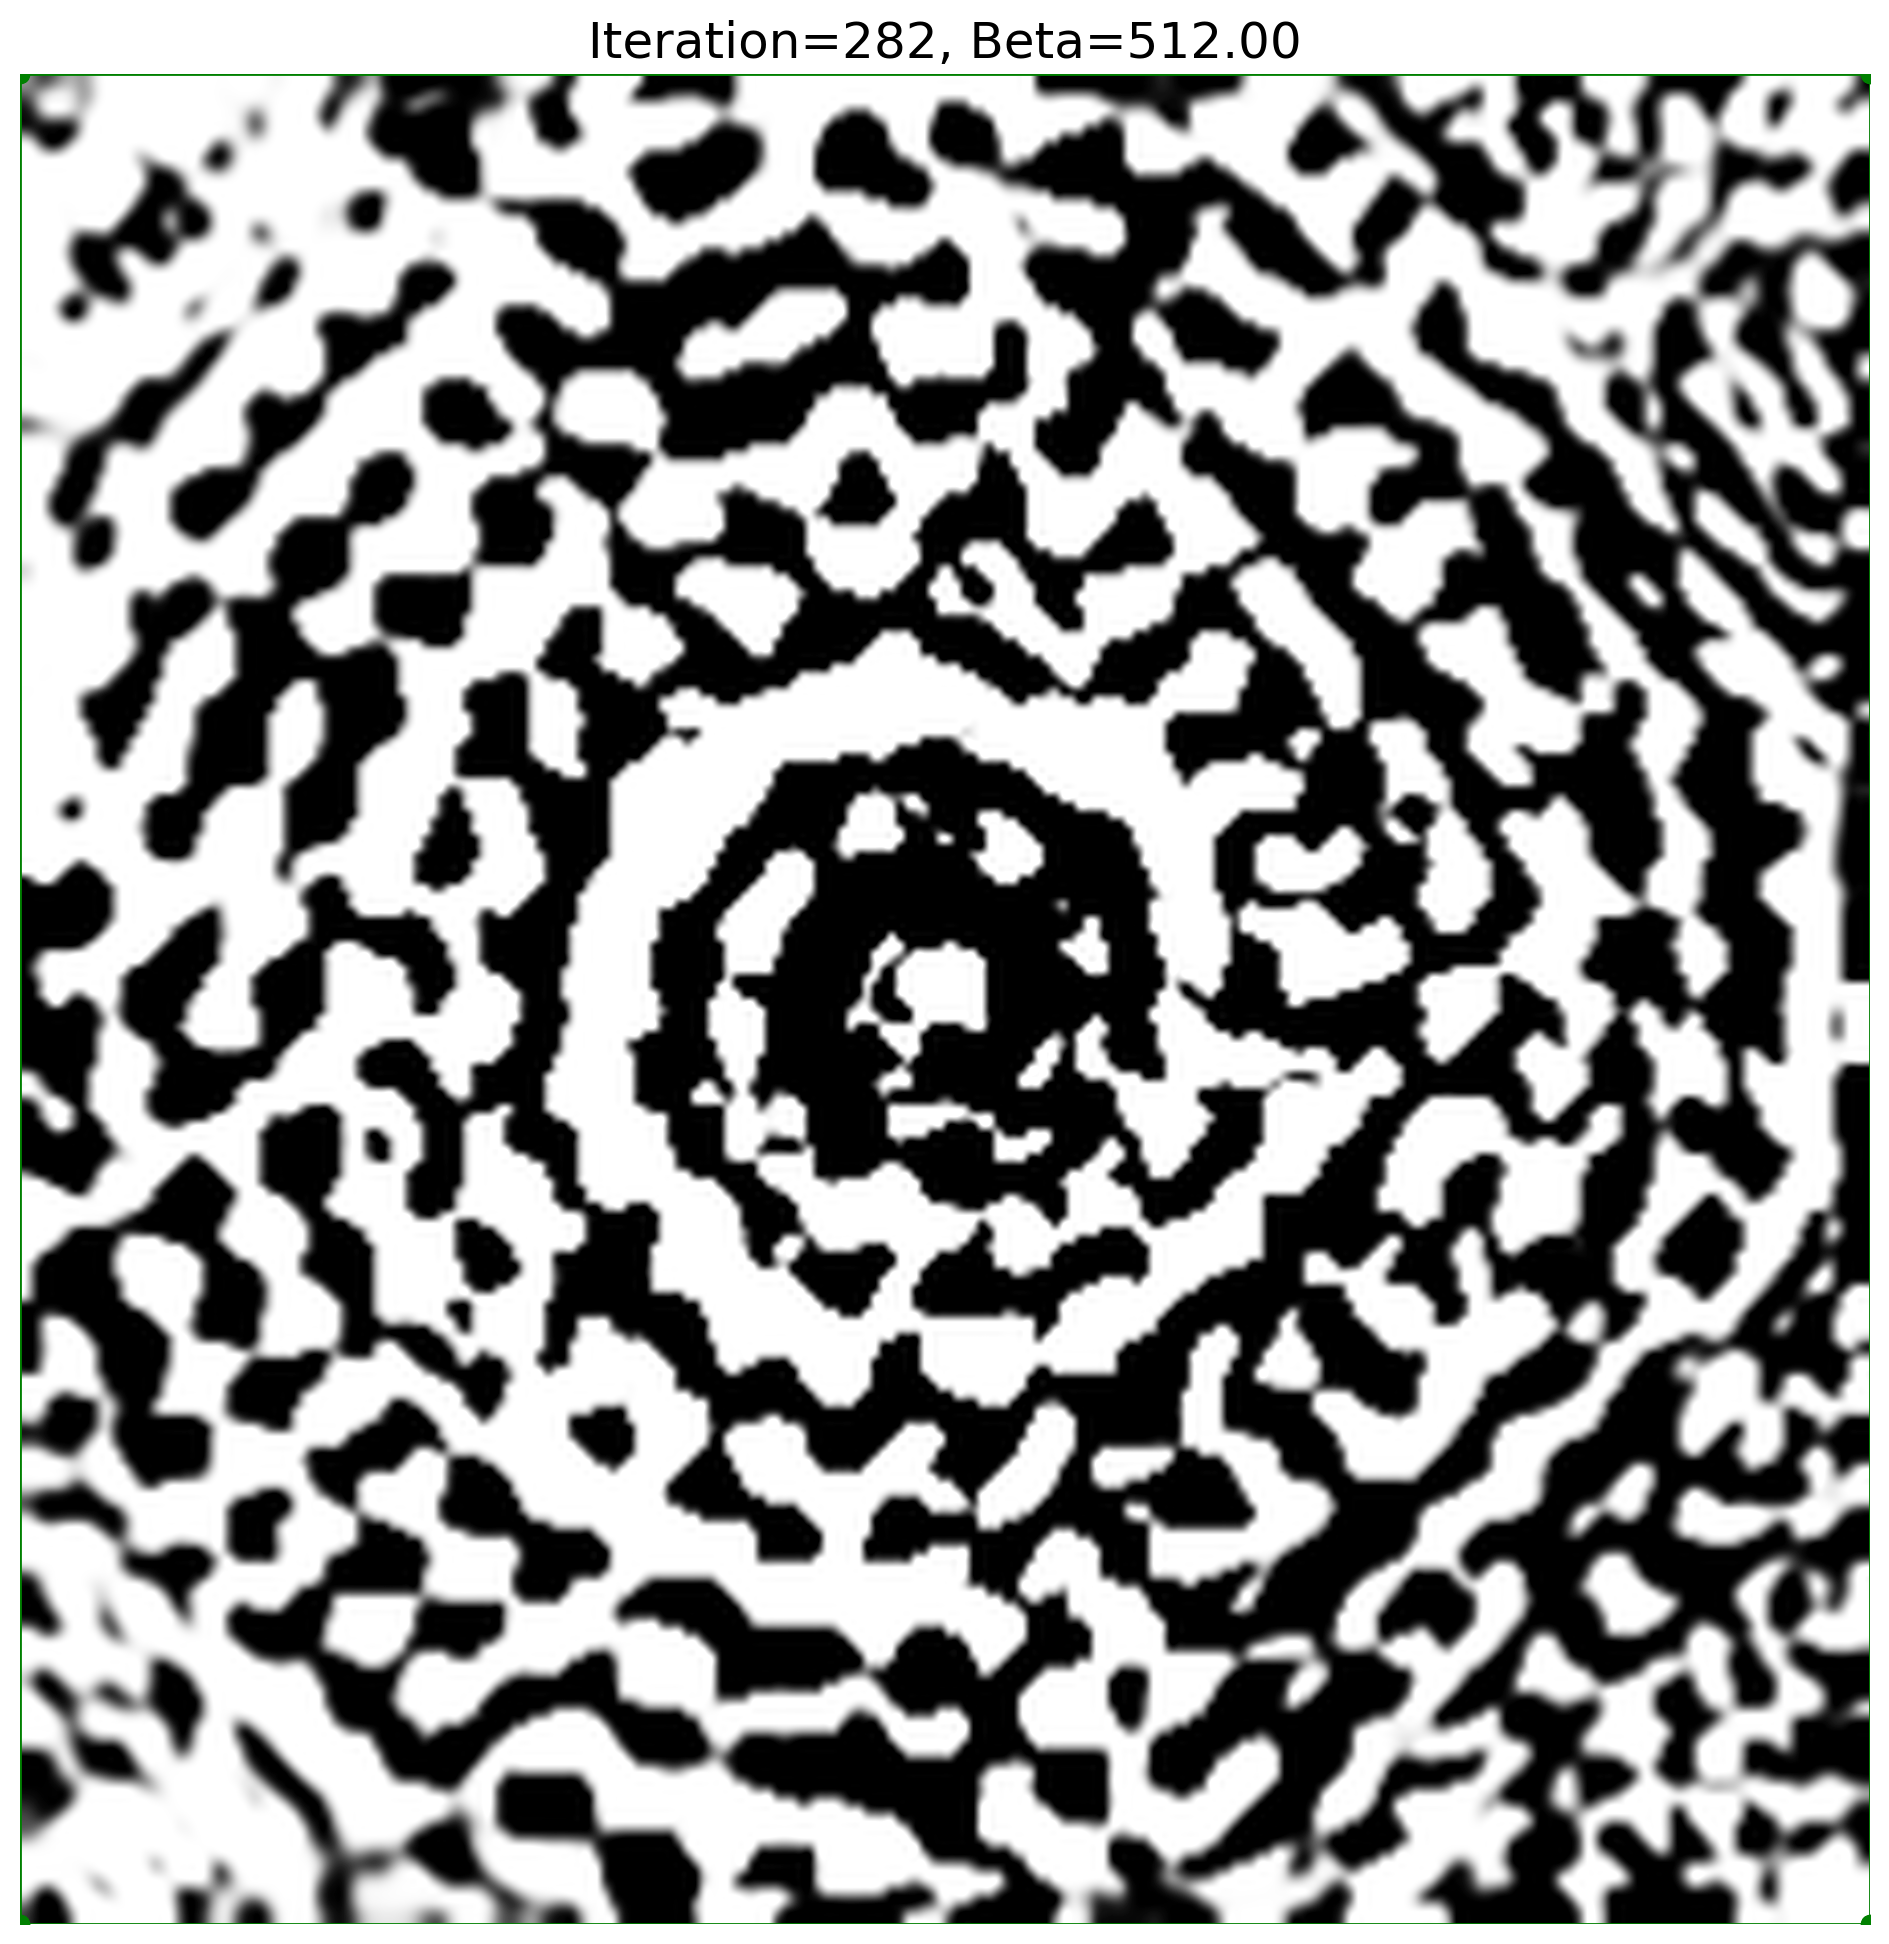
\includegraphics[width=\textwidth,height=2.4cm,keepaspectratio]{img/018_structure_iter_282_beta_512.00.png}\\
      {\tiny Optimized structure ($\ell=1$)}
    \column{0.38\textwidth}
      \centering
      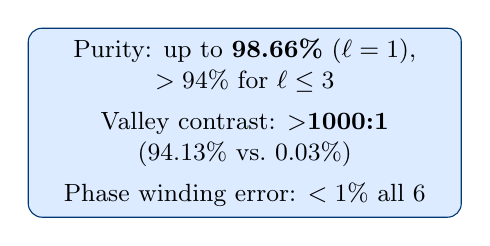
\begin{tikzpicture}
        \node[draw=NYCUblue,fill=lightblue,rounded corners=5pt,minimum width=5.5cm,minimum height=2.4cm,font=\small,align=center]{Purity: up to \textbf{98.66\%} ($\ell=1$),\\ $>94\%$ for $\ell\le3$\\[4pt] Valley contrast: \textbf{$>$1000:1}\\ (94.13\% vs.\ 0.03\%)\\[4pt] Phase winding error: \textbf{$<1\%$} all 6};
      \end{tikzpicture}
    \column{0.30\textwidth}
      \centering
      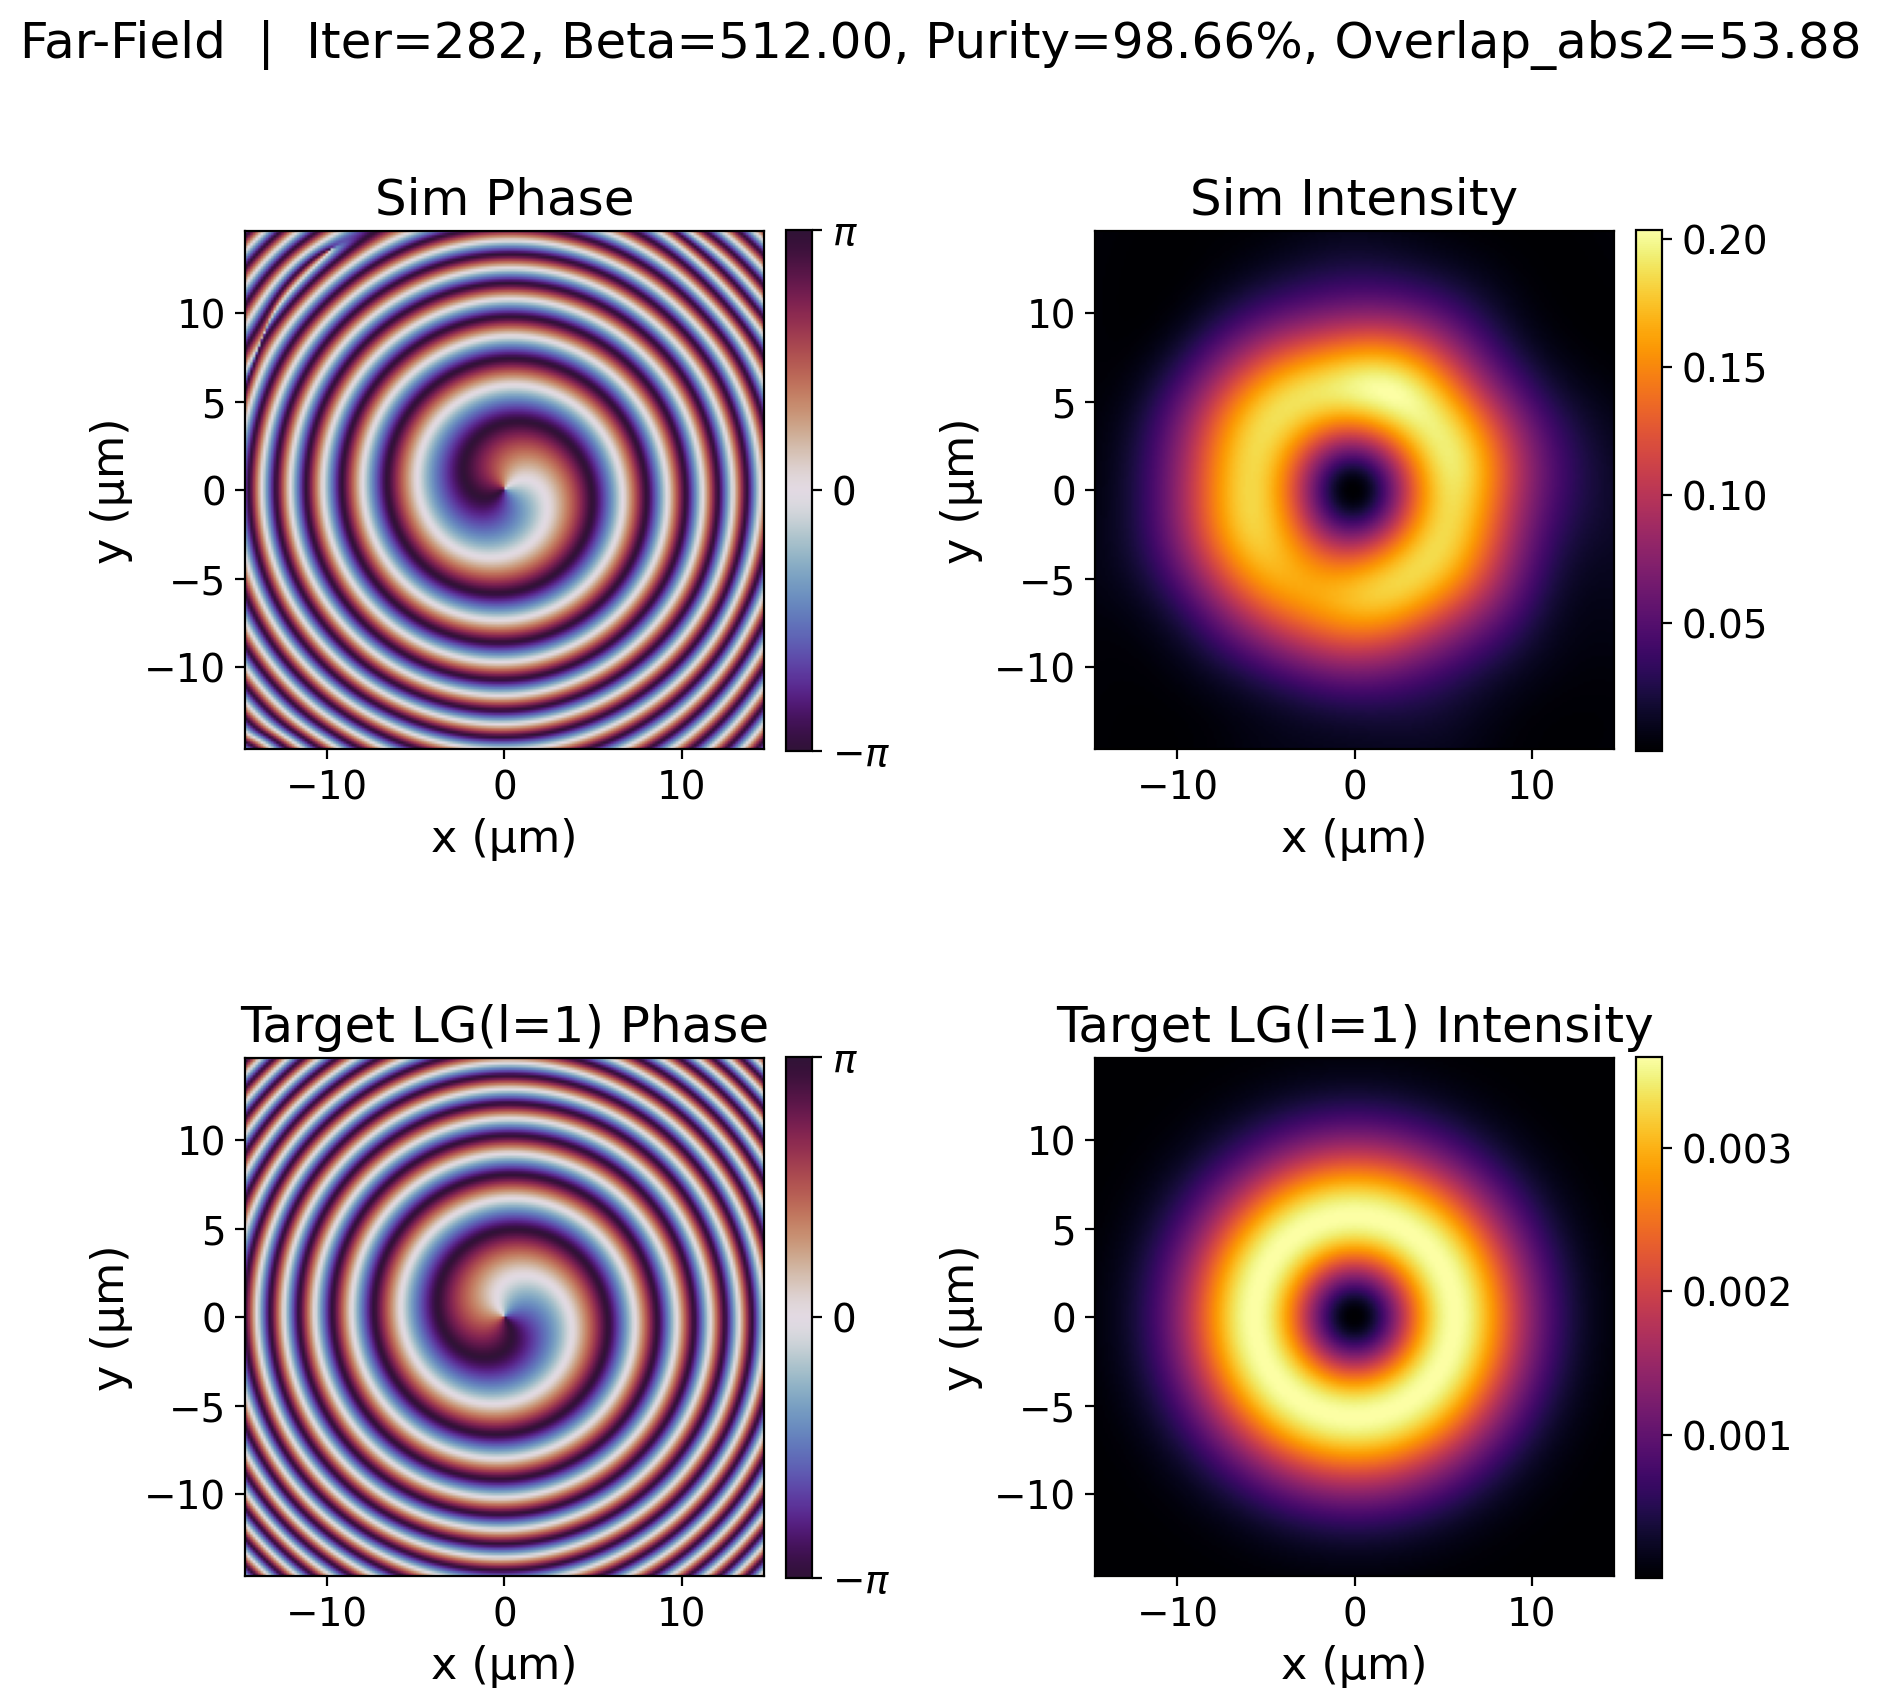
\includegraphics[width=\textwidth,height=2.4cm,keepaspectratio]{img/018_ff_iter_282_beta_512.00.png}\\
      {\tiny Far-field LG$_{1,0}$ (98.66\%)}
  \end{columns}
\end{frame}

  

% Backup Slides

\appendix

% ------------------------------------------------------------
% Backup: Extended literature preserved from the original three
% timeline tables.
% ------------------------------------------------------------

\begin{frame}{Backup: Extended Literature I --- Metasurface-Based OAM Generation}
  \begin{columns}[T]
    \column{0.90\textwidth}
      \small\renewcommand{\arraystretch}{1.15}
      \begin{tabularx}{\linewidth}{>{\bfseries}c X c}
        \toprule
        Year & Key Contribution & Purity \\
        \midrule
        \rowcolor{lightblue}
        2014 & Karimi --- L-shaped Au arrays, geometric-phase OAM (visible) & $\sim$64\% \\
        2016 & Guo --- combined geometric + propagation phase, continuous shape & $>$90\% \\
        \rowcolor{lightblue}
        2017 & Liu --- \textit{perfect vortex} (ring size $\perp \ell$) & --- \\
        2018 & Bi --- metasurface OAM multiplexing in mm-wave & --- \\
        \rowcolor{lightblue}
        2020 & Sroor --- TiO$_2$ inside laser cavity; $\ell=100$ & $\sim$90\% \\
        2021 & Zhou --- TiO$_2$ perfect vortex, tunable ring and ellipticity & --- \\
        \bottomrule
      \end{tabularx}
  \end{columns}
\end{frame}

\begin{frame}{Backup: Extended Literature II --- Valley-Chiral Photonics}
  \begin{columns}[T]
    \column{0.90\textwidth}
      \small\renewcommand{\arraystretch}{1.15}
	  \begin{tabularx}{\linewidth}{>{\bfseries}c X}
        \toprule
        Year & Key Contribution \\
        \midrule
        \rowcolor{lightblue}
        2012 & Mak, Zeng --- experimental valley polarization in MoS$_2$ / WSe$_2$ \\
        2013 & Gan --- first 2D material on GaP photonic crystal microcavity \\
        \rowcolor{lightblue}
        2018 & Gong --- $\text{WS}_2$ + Ag nanowire; valley directional coupling 90\% \\
        2019 & Sortino --- GaP nanoantenna + WSe$_2$; PL enhancement $10^4\times$ \\
        \rowcolor{lightblue}
        2020 & Rong --- Si metasurface, photonic Rashba; directional valley beam \\
        2025 & Pan --- Si chiral metasurface + quasi-BIC; room-T valley-selective CP \\
        \bottomrule
      \end{tabularx}
  \end{columns}
\end{frame}

\begin{frame}{Backup: Extended Literature III --- Inverse-Designed Nanophotonics}
  \begin{columns}[T]
    \column{0.90\textwidth}
      \small\renewcommand{\arraystretch}{1.15}
	  \begin{tabularx}{\linewidth}{>{\bfseries}c X}
        \toprule
        Year & Key Contribution \\
        \midrule
        \rowcolor{lightblue}
        2011 & Jensen --- topology optimization framework for nanophotonics \\
        2022 & Li --- topology-optimized metasurface, asymmetric beam deflection \\
        \rowcolor{lightblue}
        2023 & Gelly --- inverse design + TMD for cavity coupling \\
        2023 & White --- inverse-designed Si OAM emitter (passive; no valley selectivity) \\
        \rowcolor{lightblue}
        2024 & Wang --- full-Stokes polarimetry via inverse-designed metasurface \\
        2025 & Choi --- large-NA achromatic metalens by inverse design \\
        \bottomrule
      \end{tabularx}
  \end{columns}
\end{frame}



% ------------------------------------------------------------
% Backup: Pancharatnam-Berry phase formalism (removed from main
% deck; preserved here in case committee asks about the
% resemblance noted on the Structures slide).
% ------------------------------------------------------------

\begin{frame}{Backup: SAM $\to$ OAM, Pancharatnam--Berry Phase}
  \begin{columns}[T]
    \column{0.52\textwidth}
      \begin{block}{Geometric (PB) Phase}
        Nanoantenna rotated by $\theta$:
        $\Phi_{\rm PB} = 2 \sigma \theta$, 
        $\sigma = \pm 1$: incident circular polarization.
        \begin{itemize}
          \item Opposite SAM states $\to$ opposite geometric phases
          \item Phase set by geometry, not material dispersion
        \end{itemize}
      \end{block}
      \vspace{1pt}
      \begin{exampleblock}{OAM Encoding}
		Rotation angle:
		$\theta(\phi)=q\phi$
		PB phase:
		$\Phi_{PB}=2\sigma q\phi$
		Equivalent helical phase:
		$e^{i\ell\phi},\qquad \ell=2\sigma q.$
      \end{exampleblock}
      \vspace{1pt}
      \begin{alertblock}{Relation to This Work}
        This work does \textbf{not} prescribe $\theta(\phi)$: topology optimization finds the phase profile freely. Emergent spiral geometry (Structures slide) qualitatively resembles a PB-phase pattern as a byproduct, not a design choice.
      \end{alertblock}
    \column{0.45\textwidth}
      \centering
      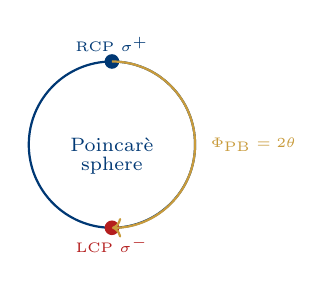
\begin{tikzpicture}[scale=0.88, font=\footnotesize]
        \draw[thick, NYCUblue] (0,0) circle (1.2);
        \fill[NYCUblue]  (0, 1.2) circle (3pt) node[above]{\tiny RCP $\sigma^+$};
        \fill[accentred] (0,-1.2) circle (3pt) node[below]{\tiny LCP $\sigma^-$};
        \draw[NYCUgold, thick, ->](0,1.2) arc[start angle=90,end angle=-90,radius=1.2] node[midway,right=2pt]{\tiny $\Phi_{\rm PB}=2\theta$};
        \node[NYCUblue,font=\scriptsize] at (0, 0.0) {Poincar\`{e}};
        \node[NYCUblue,font=\scriptsize] at (0,-0.3) {sphere};
      \end{tikzpicture}
  \end{columns}
\end{frame}



\begin{frame}{Backup: LG Mode Definition \& Performance Metrics}

  \[ u_{p,\ell}(r,\phi,z) = \sqrt{\frac{2p!}{\pi(p+|\ell|)!}} \frac{1}{w}\!\left(\frac{\sqrt{2}r}{w}\right)^{|\ell|} L_p^{|\ell|}\!\!\left(\frac{2r^2}{w^2}\right) e^{-r^2/w^2}\,e^{ikr^2/2R}\,e^{i\ell\phi}\,e^{-i(2p+|\ell|+1)\psi} \]

  \begin{columns}[T]
    \column{0.48\textwidth}
      \begin{block}{Overlap Integral}
        \[ \text{Overlap}=\int_A(E_{ff,x}E_{t,x}^*+E_{ff,y}E_{t,y}^*)\,dA \]
      \end{block}
    \column{0.48\textwidth}
      \begin{block}{Mode Purity}
        \[ \text{Purity}=\frac{|\text{Overlap}|^2}{P_{\rm sim}\cdot P_{\rm target}},\;P_{\rm target}=1 \]
      \end{block}
  \end{columns}
  \vspace{1pt}
  \begin{block}{Phase Winding \& Chirality}
    Winding: sample $\phi(r_{\rm peak},\theta)$, unwrap, compare with $\ell\times2\pi$.\\
    Chirality: $C=\pi f\,\mathrm{Im}(\mathbf{E}^*\cdot\mathbf{H})$.
  \end{block}
\end{frame}

  

\begin{frame}{Backup: Valley Selection Rule}
  Under $D_{3h}$ symmetry:
  \[ |\langle u_{c,K}|\hat{p}_+|u_{v,K}\rangle|^2\neq0,\quad |\langle u_{c,K}|\hat{p}_-|u_{v,K}\rangle|^2=0 \]
  \[ |\langle u_{c,K'}|\hat{p}_-|u_{v,K'}\rangle|^2\neq0,\quad |\langle u_{c,K'}|\hat{p}_+|u_{v,K'}\rangle|^2=0 \]
  \begin{columns}[T]
    \column{0.48\textwidth}
      \begin{block}{Valley Polarization Degree}
        \[ P_c=\frac{I(\sigma^+)-I(\sigma^-)}{I(\sigma^+)+I(\sigma^-)} \]
        Experimentally: 20--50\% at RT; Purcell $\to\sim80\%$
      \end{block}
    \column{0.48\textwidth}
      \begin{alertblock}{Impact on Experiment}
        \[ \text{Purity}_{\rm exp}\approx P_c^2\times\text{Purity}_{\rm sim} \]
        $P_c=80\%$: Purity$_{\rm exp}\approx63\%$
      \end{alertblock}
  \end{columns}
\end{frame}

  

\begin{frame}{Backup: Complete Simulation Parameters}
  \centering
  \begin{tabular}{ll}
    \toprule
    \textbf{Parameter} & \textbf{Value} \\
    \midrule
    Wavelength $\lambda$ & $0.593\;\mu$m ($\text{WS}_2$ A-exciton) \\
    $n_{\rm GaP}$ & $3.31$ \\
    $n_{\rm Diamond}$ & $2.40$ \\
    Design layer $t$ & $0.257\;\mu$m \\
    Design area & $4.5\times4.5\;\mu\text{m}^2$ \\
    Resolution & $50\;\text{pts}/\mu$m \\
    Design variables $N$ & $226^2\approx5.1\times10^4$ \\
    PML thickness & $0.3\;\mu$m \\
    Min.\ feature size & $0.05\;\mu$m \\
    $\beta$ schedule & $4\to512$ (geometric then $\times2$) \\
    FOM weight $\alpha$ & $0.10$ \\
    Far-field plane & $z=10\,z_R$ \\
    Optimizer & MMA (via NLopt) \\
    Targets & 6 ($\ell=0,1,2,3,4,5$) \\
    \bottomrule
  \end{tabular}
\end{frame}

  

\begin{frame}{Backup: Near-Field Phase \& Intensity (All 6)}
  \centering
  {\footnotesize Near-field monitor plane. Each panel: phase(L)+intensity(R).}\\[4pt]

  \begin{tabular}{ccc}
    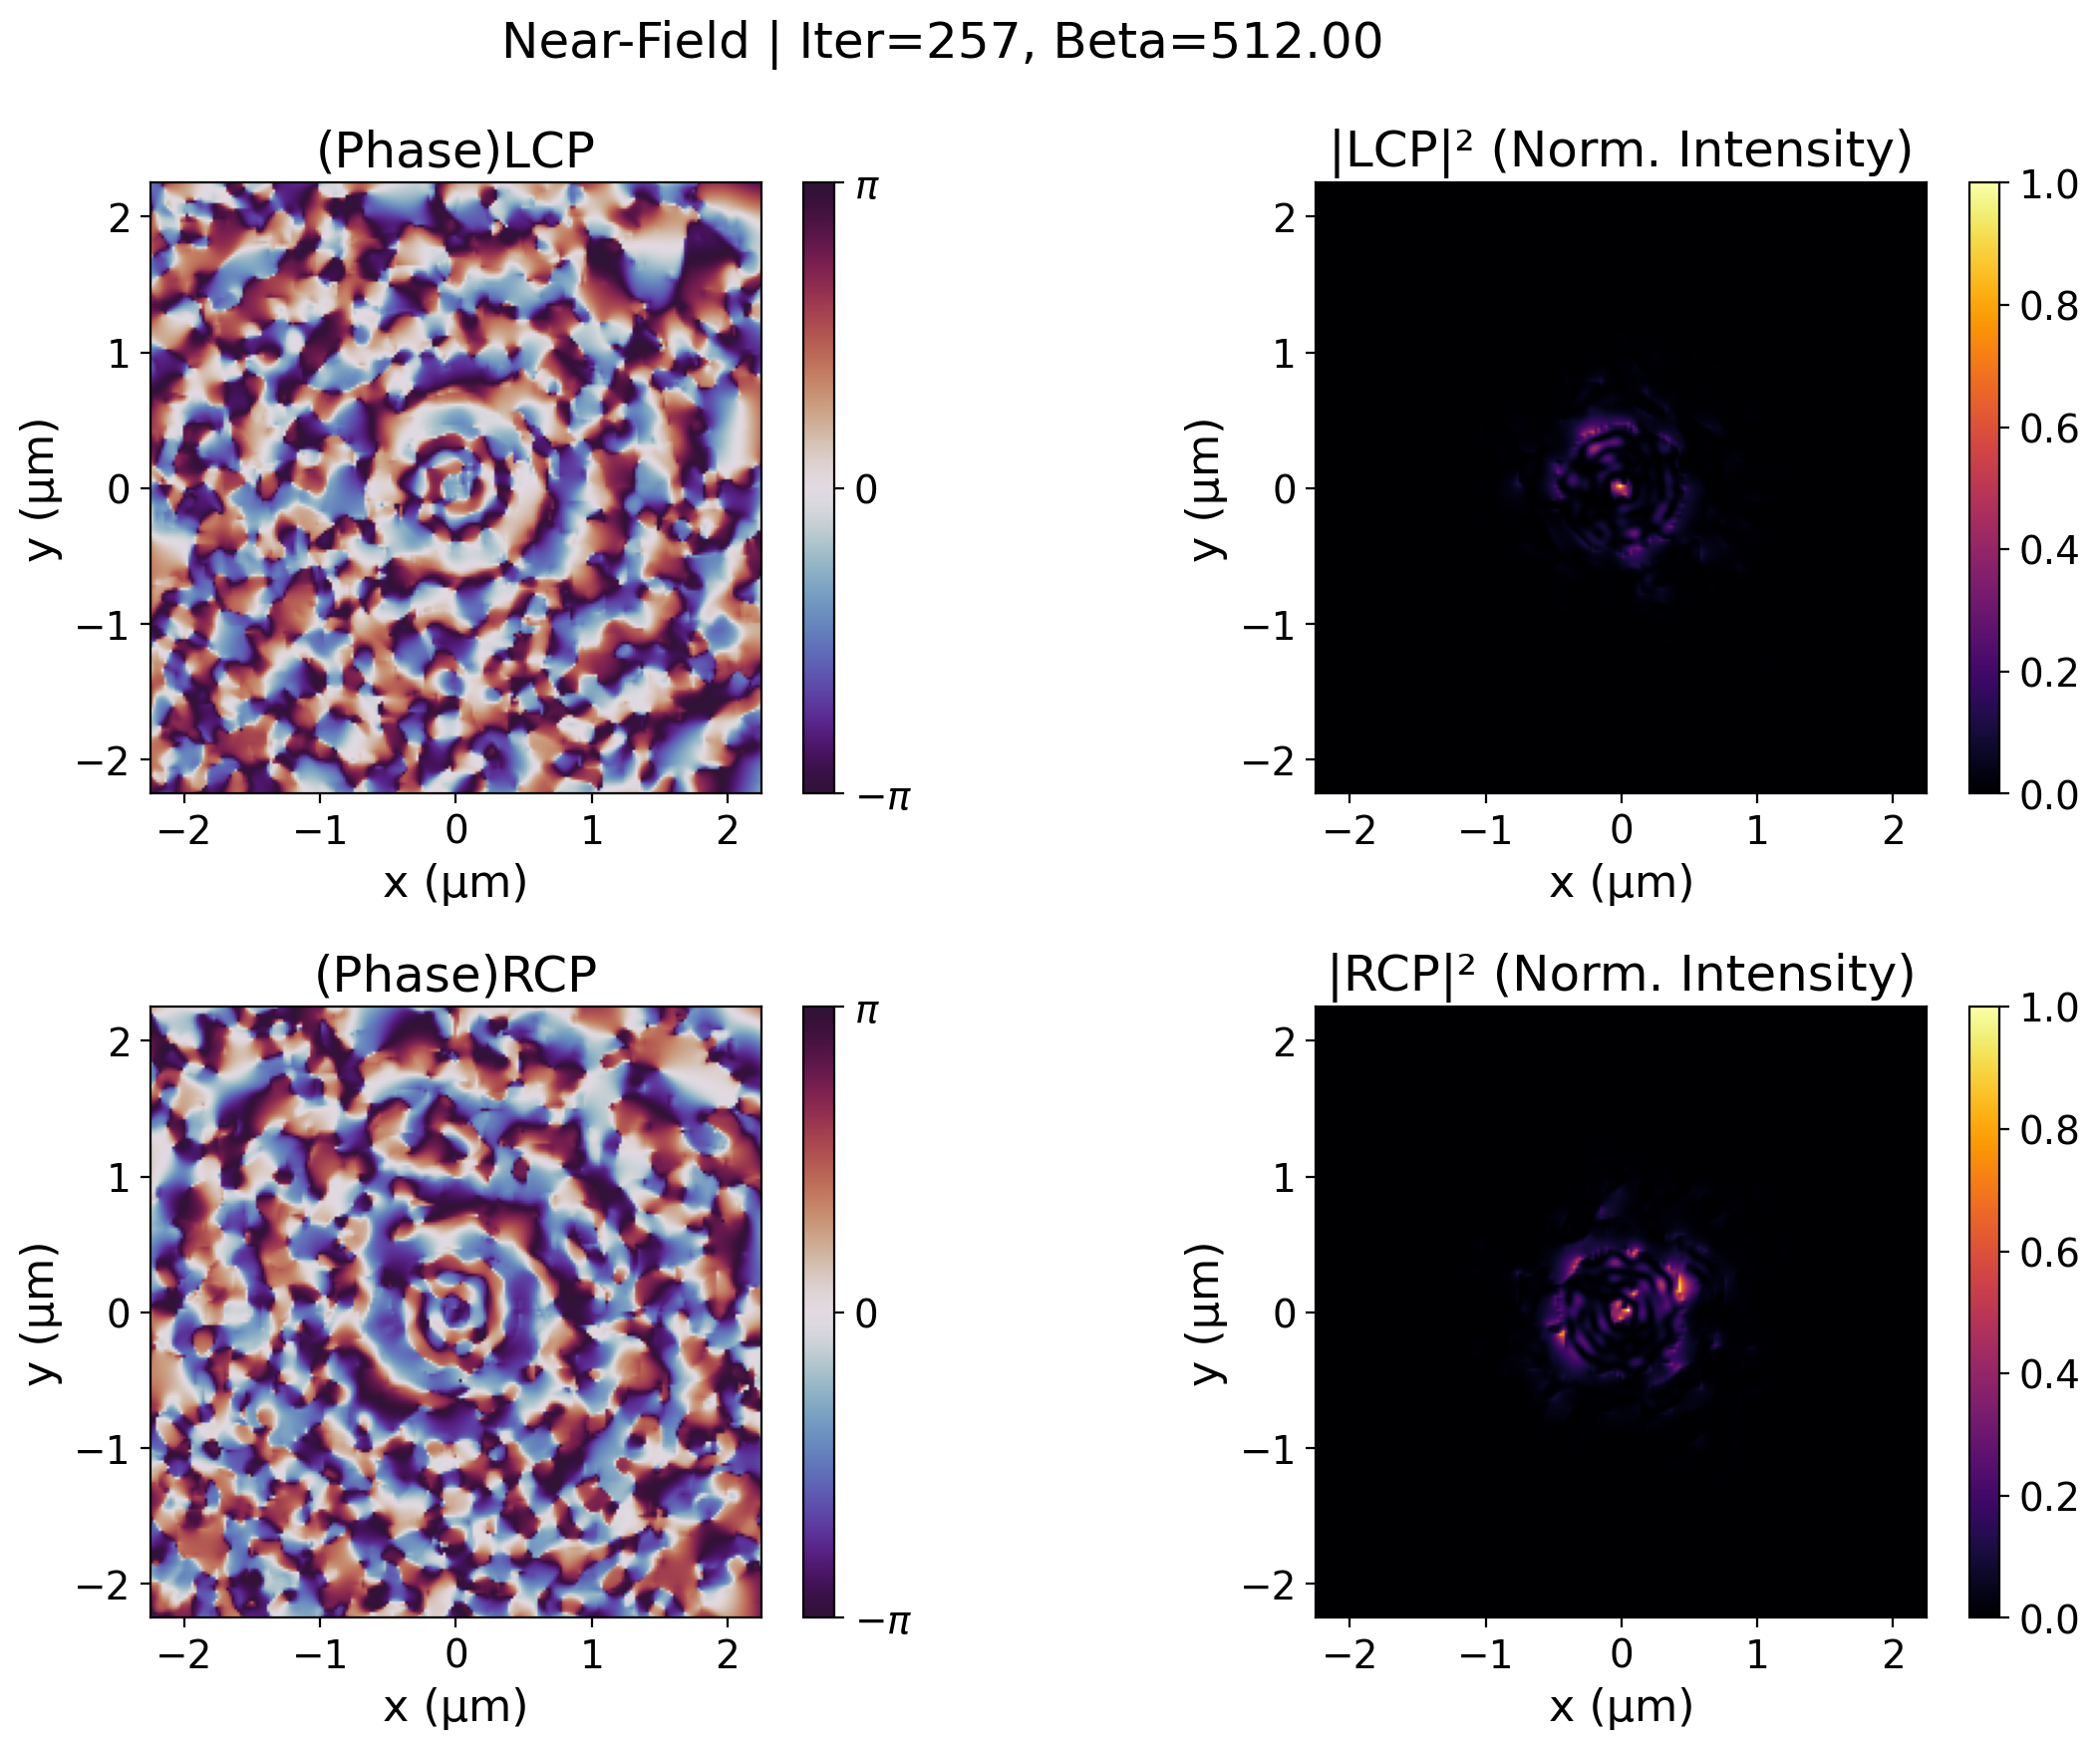
\includegraphics[width=0.31\textwidth,keepaspectratio]{img/017_phase_iter_257_beta_512.00.png} &
    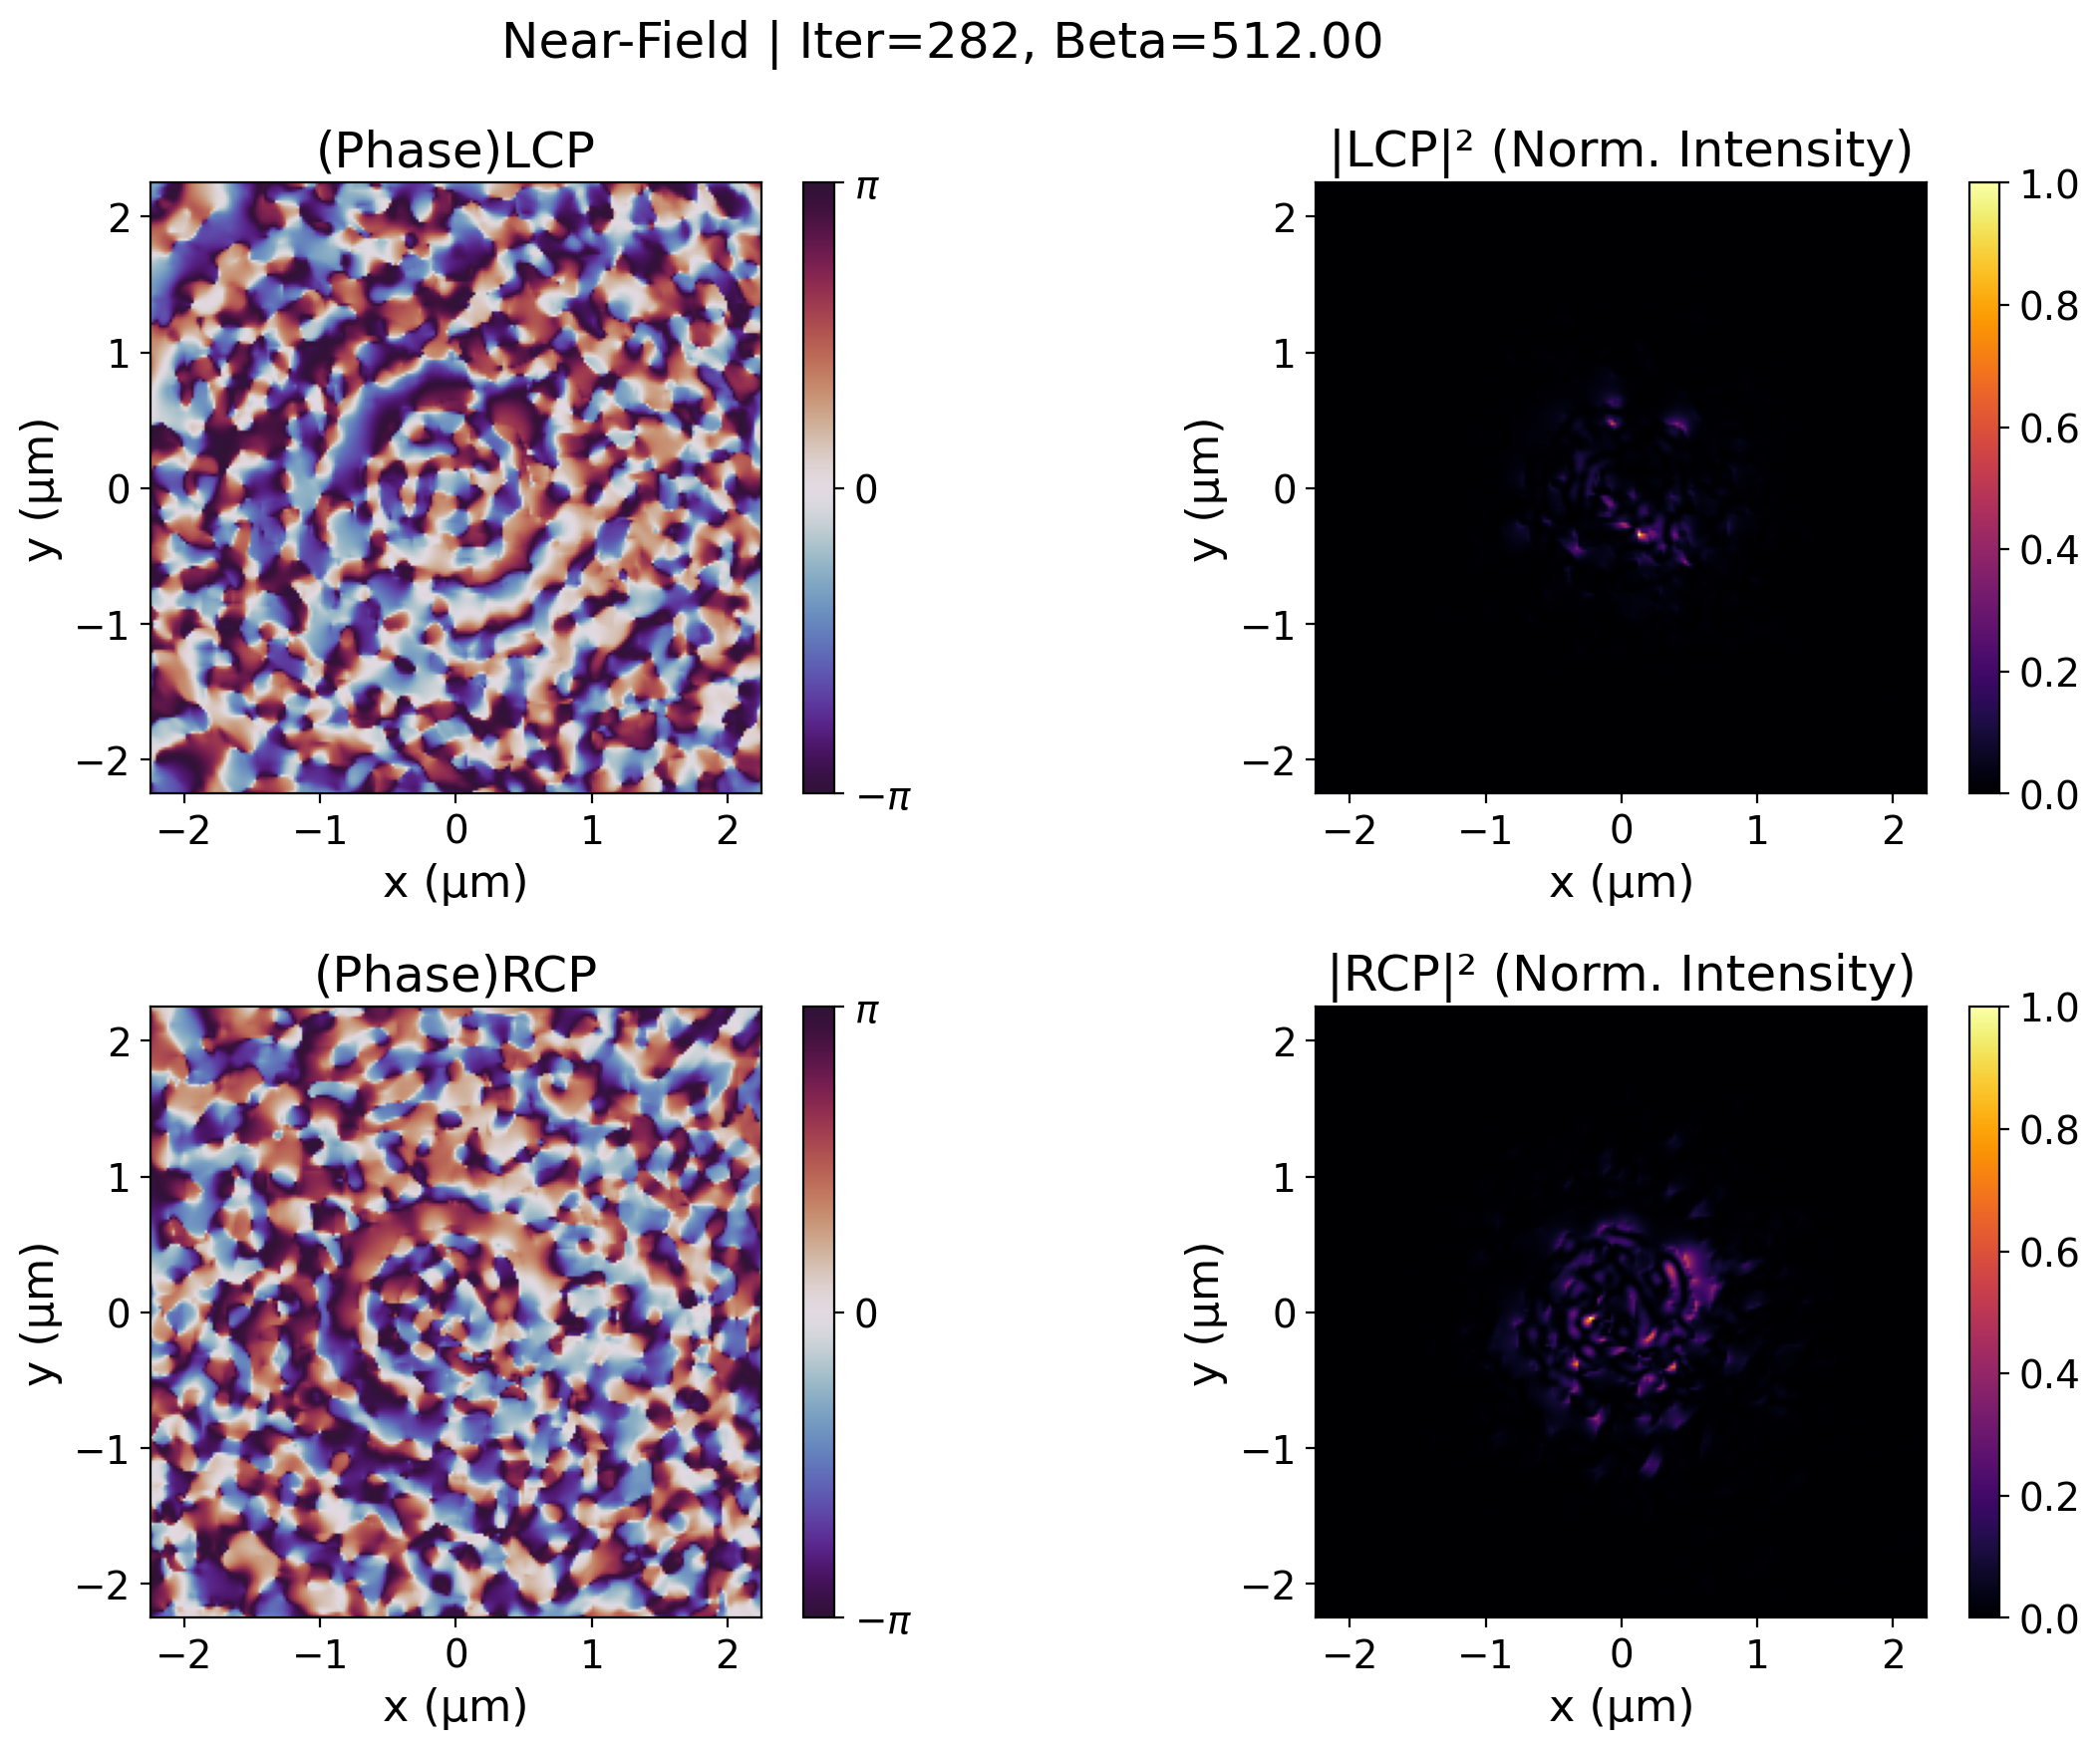
\includegraphics[width=0.31\textwidth,keepaspectratio]{img/018_phase_iter_282_beta_512.00.png} &
    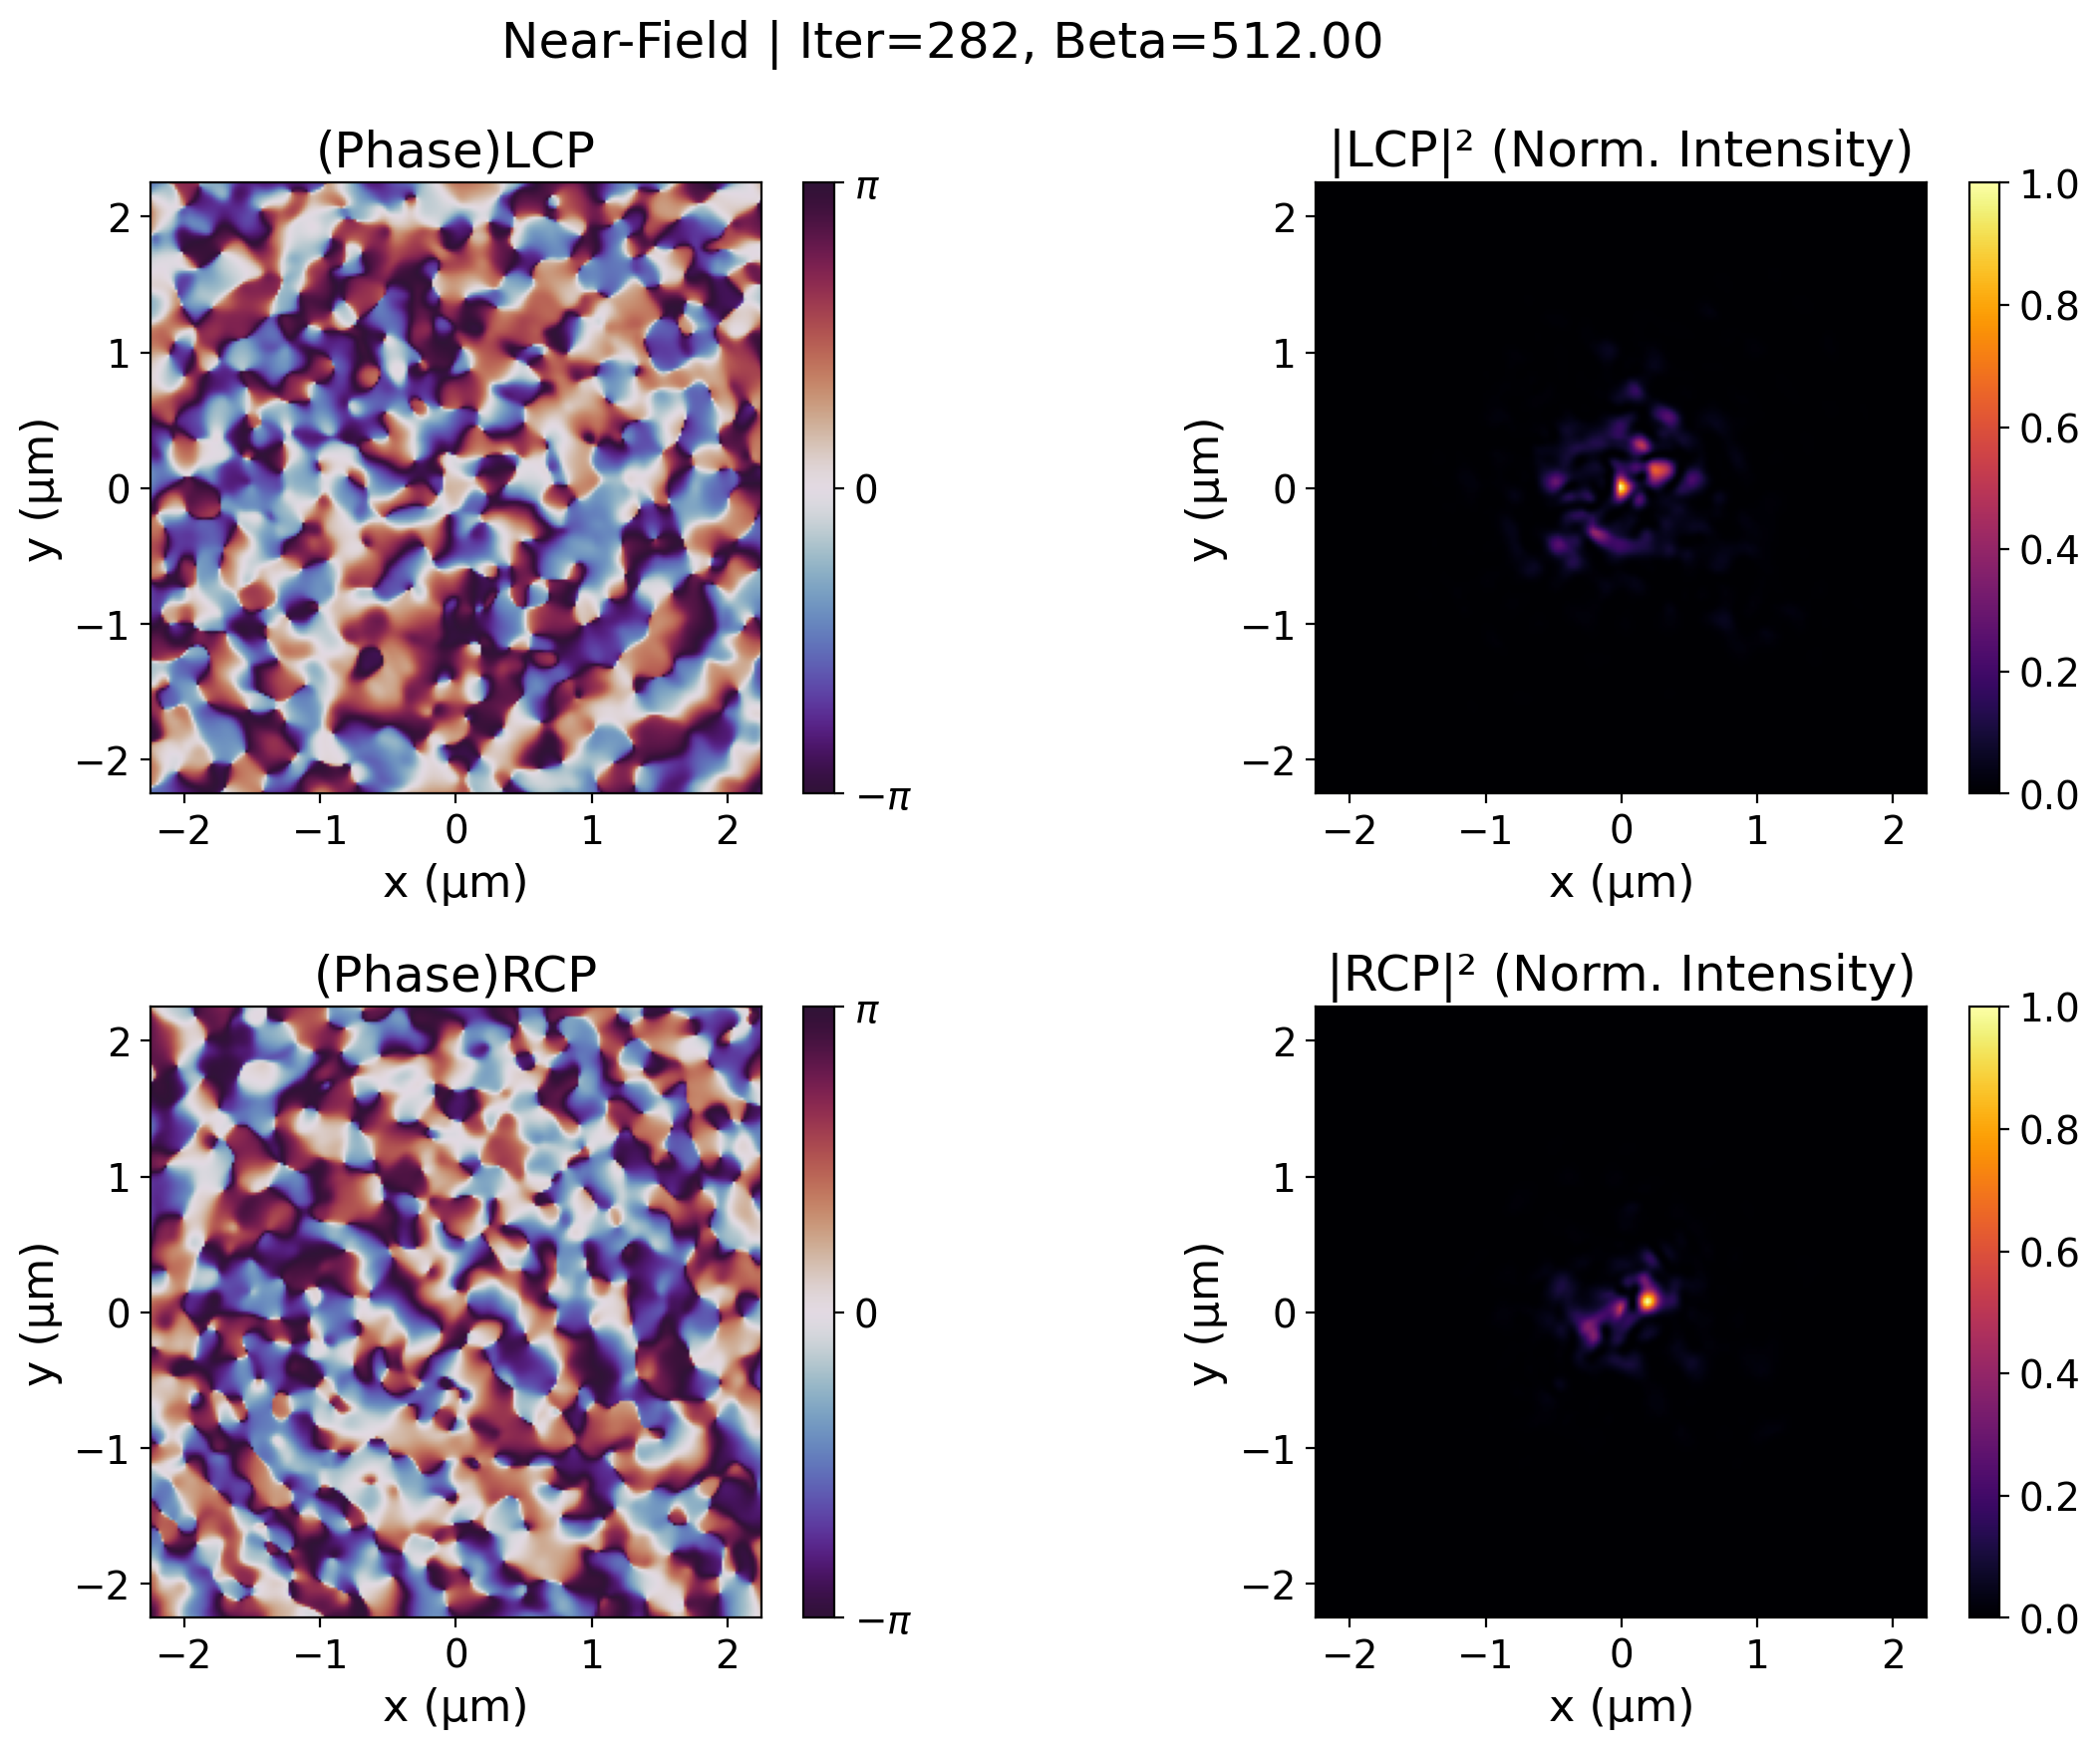
\includegraphics[width=0.31\textwidth,keepaspectratio]{img/013_phase_iter_282_beta_512.00.png} \\
    {\tiny (a) $\ell=0$} & {\tiny (b) $\ell=1$} & {\tiny (c) $\ell=2$} \\[4pt]
    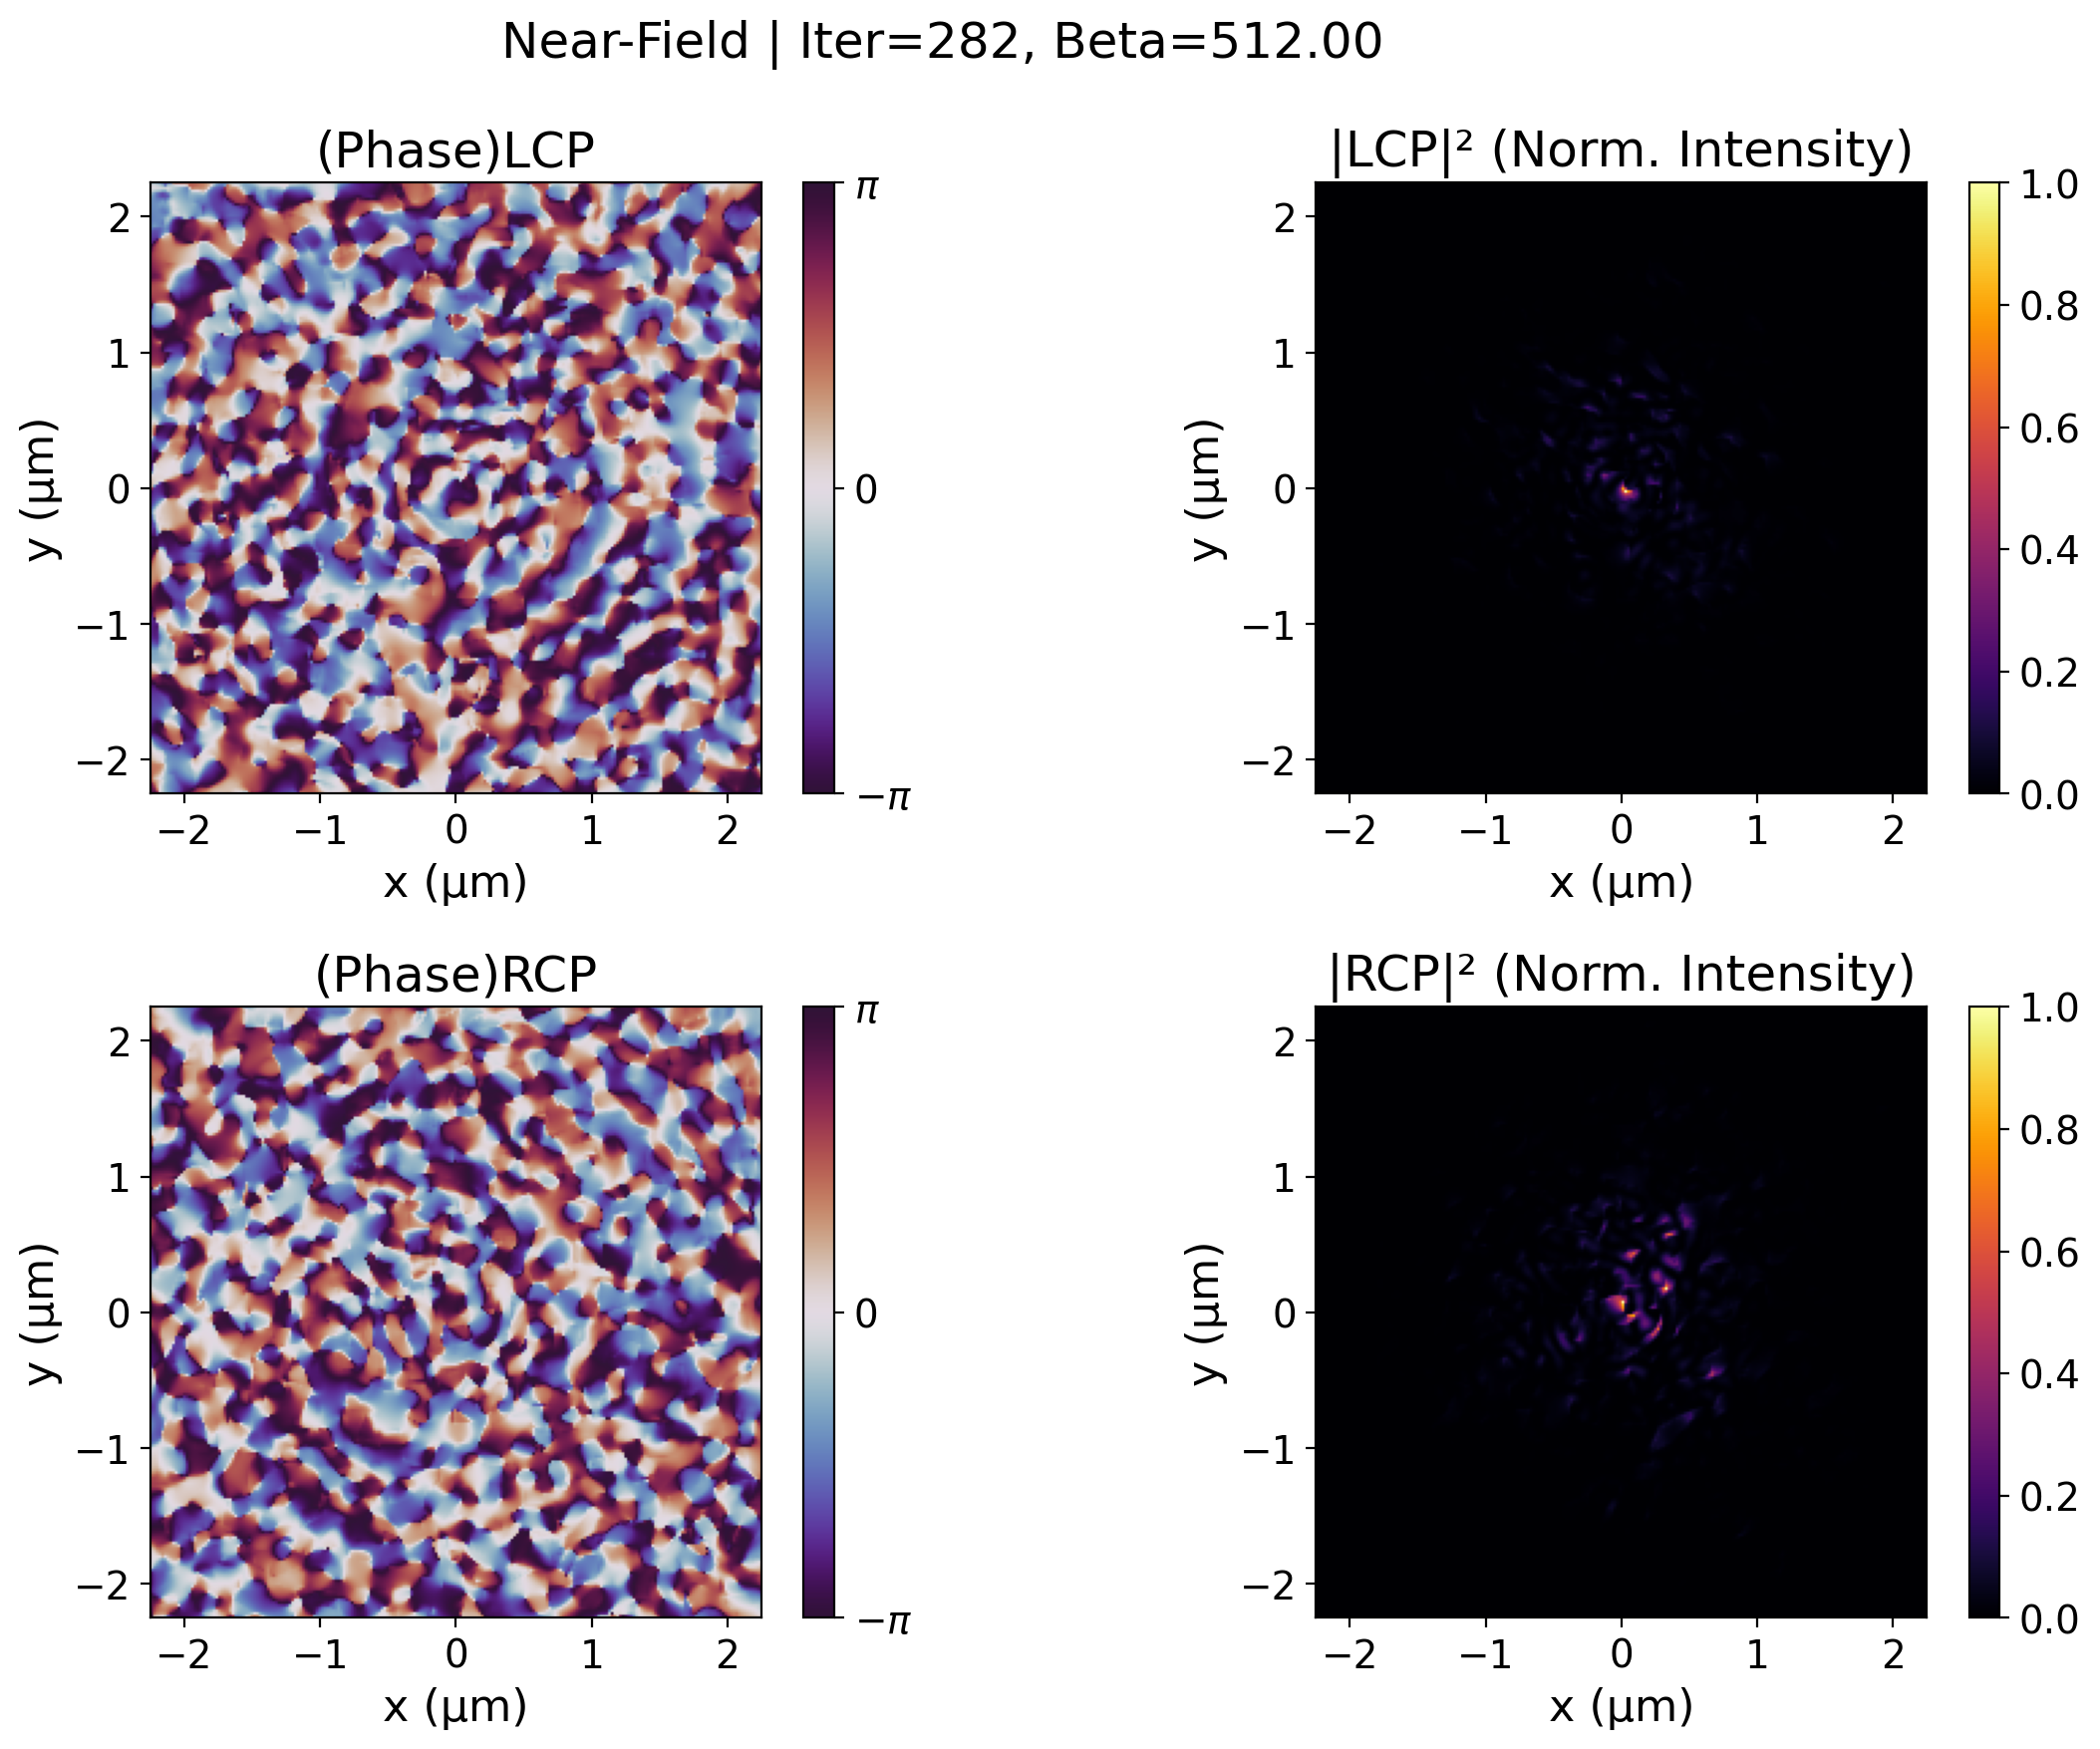
\includegraphics[width=0.31\textwidth,keepaspectratio]{img/020_phase_iter_282_beta_512.00.png} &
    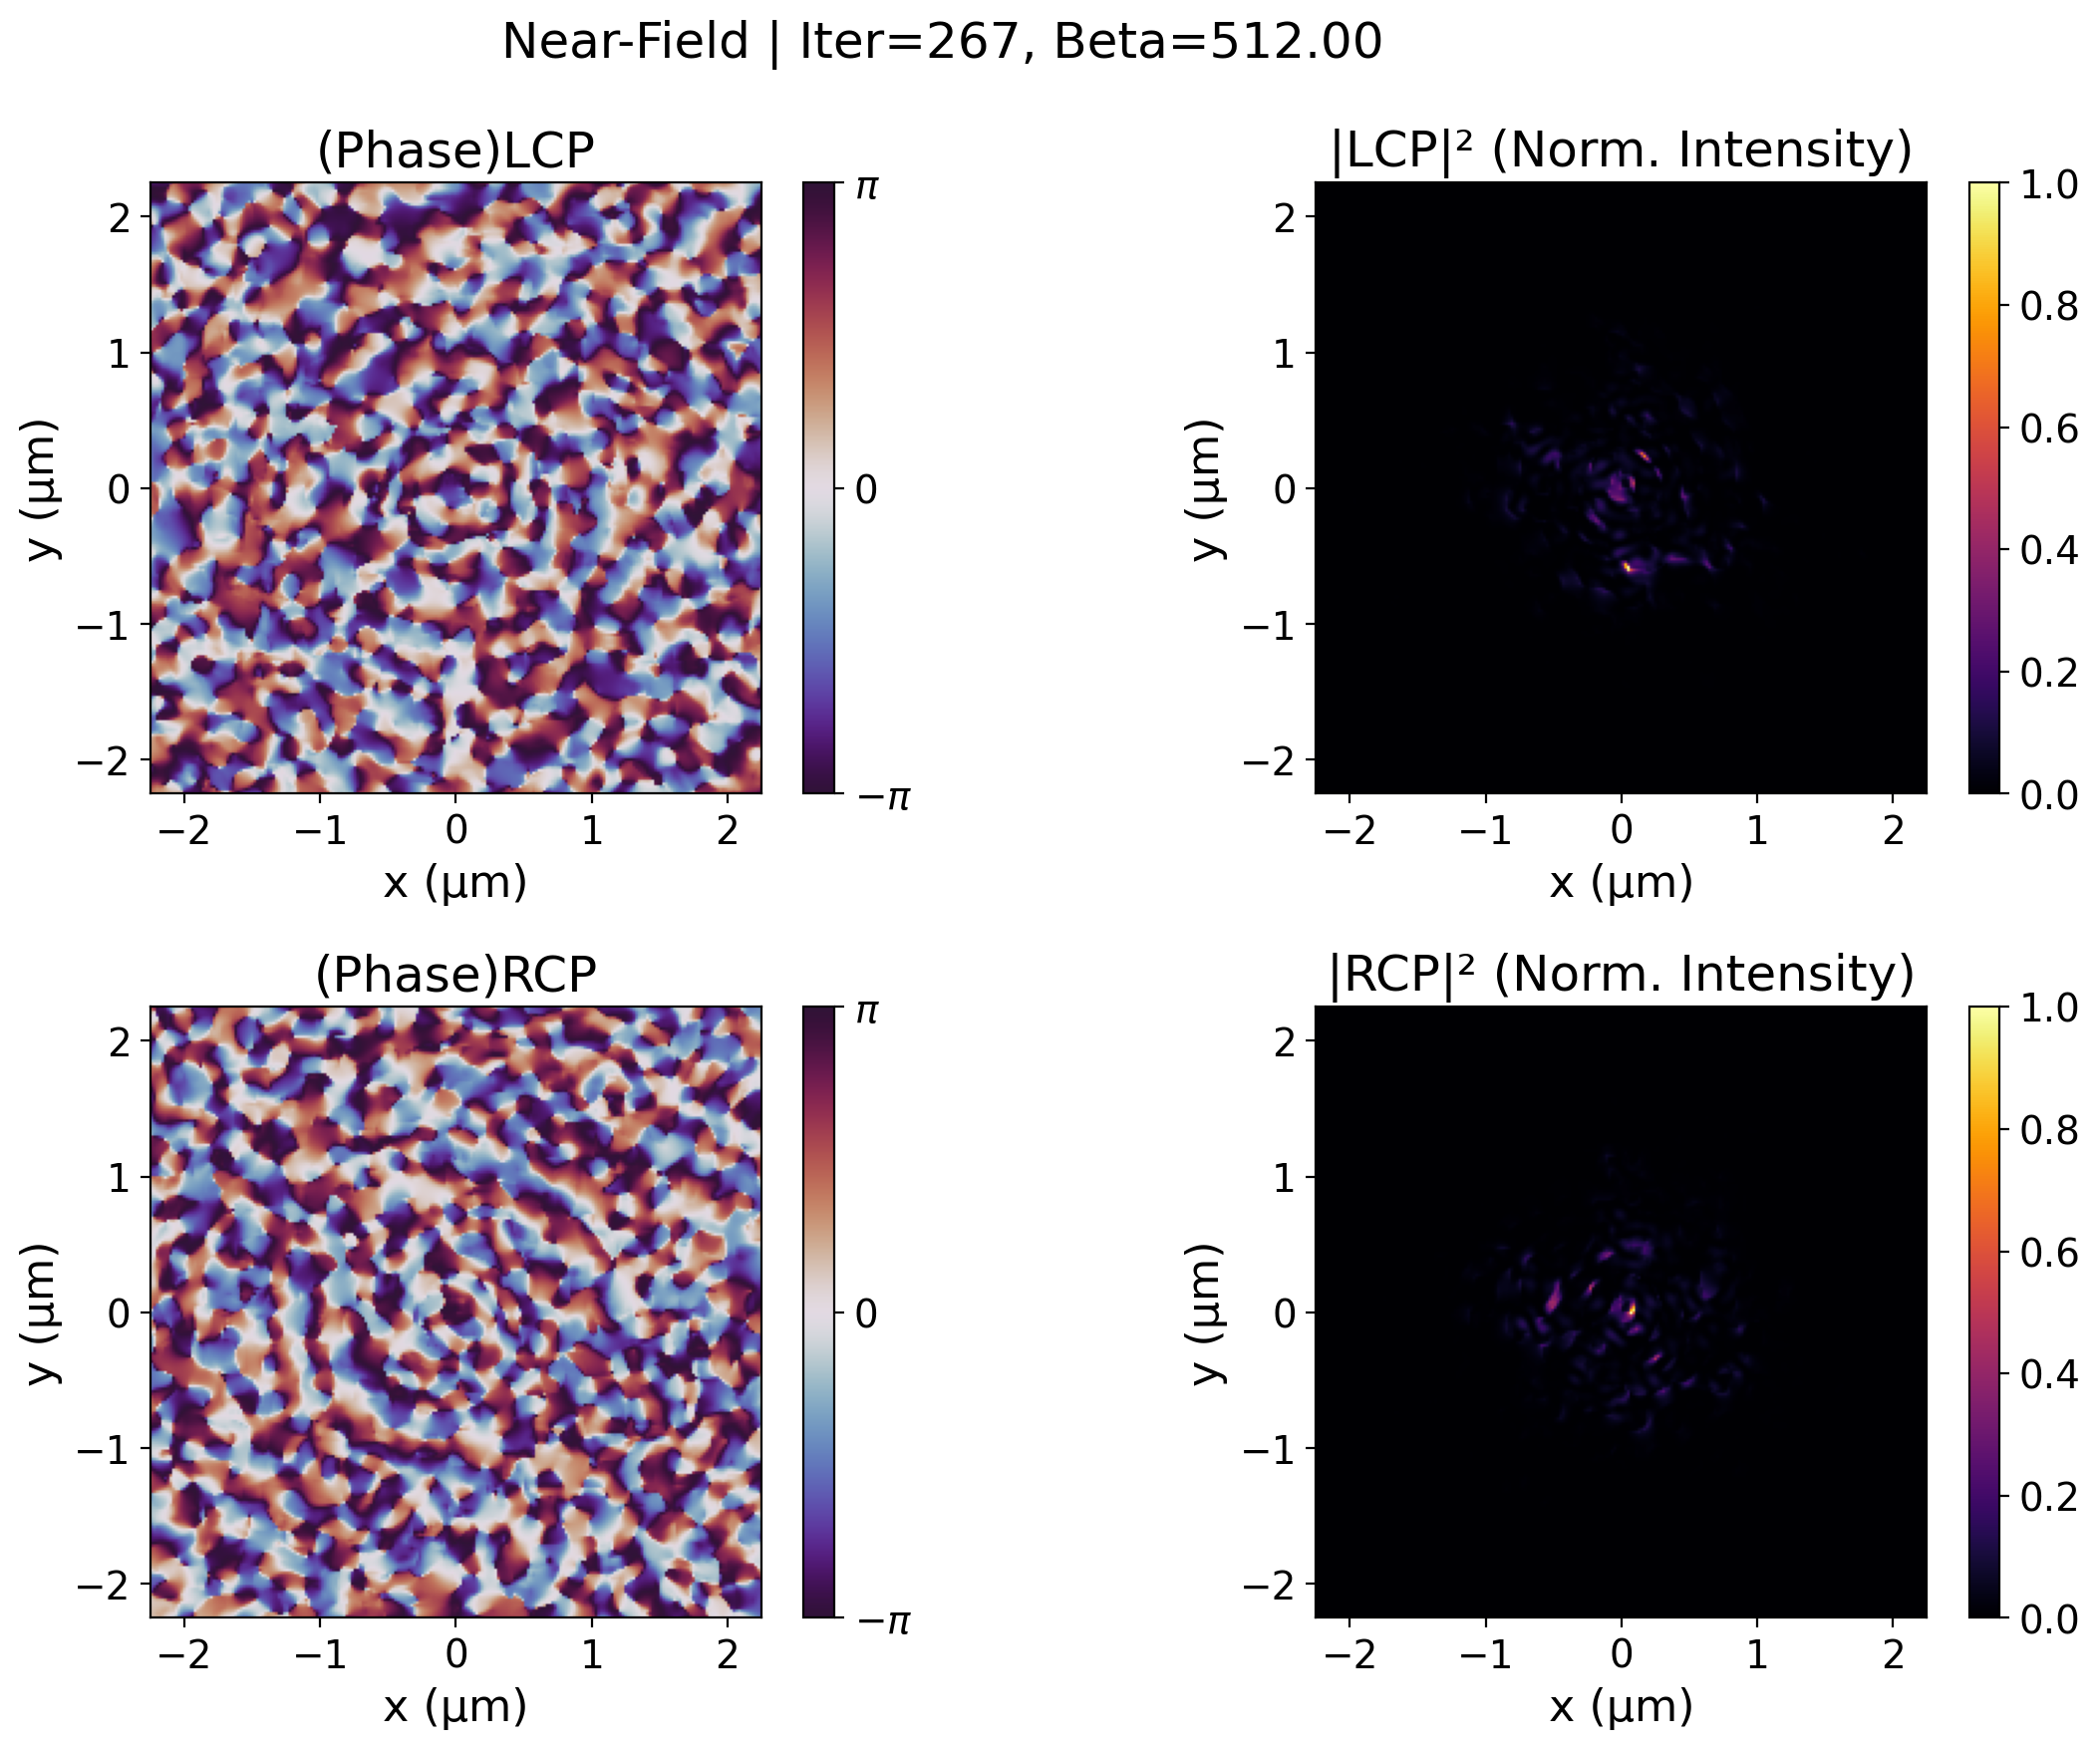
\includegraphics[width=0.31\textwidth,keepaspectratio]{img/021_phase_iter_267_beta_512.00.png} &
    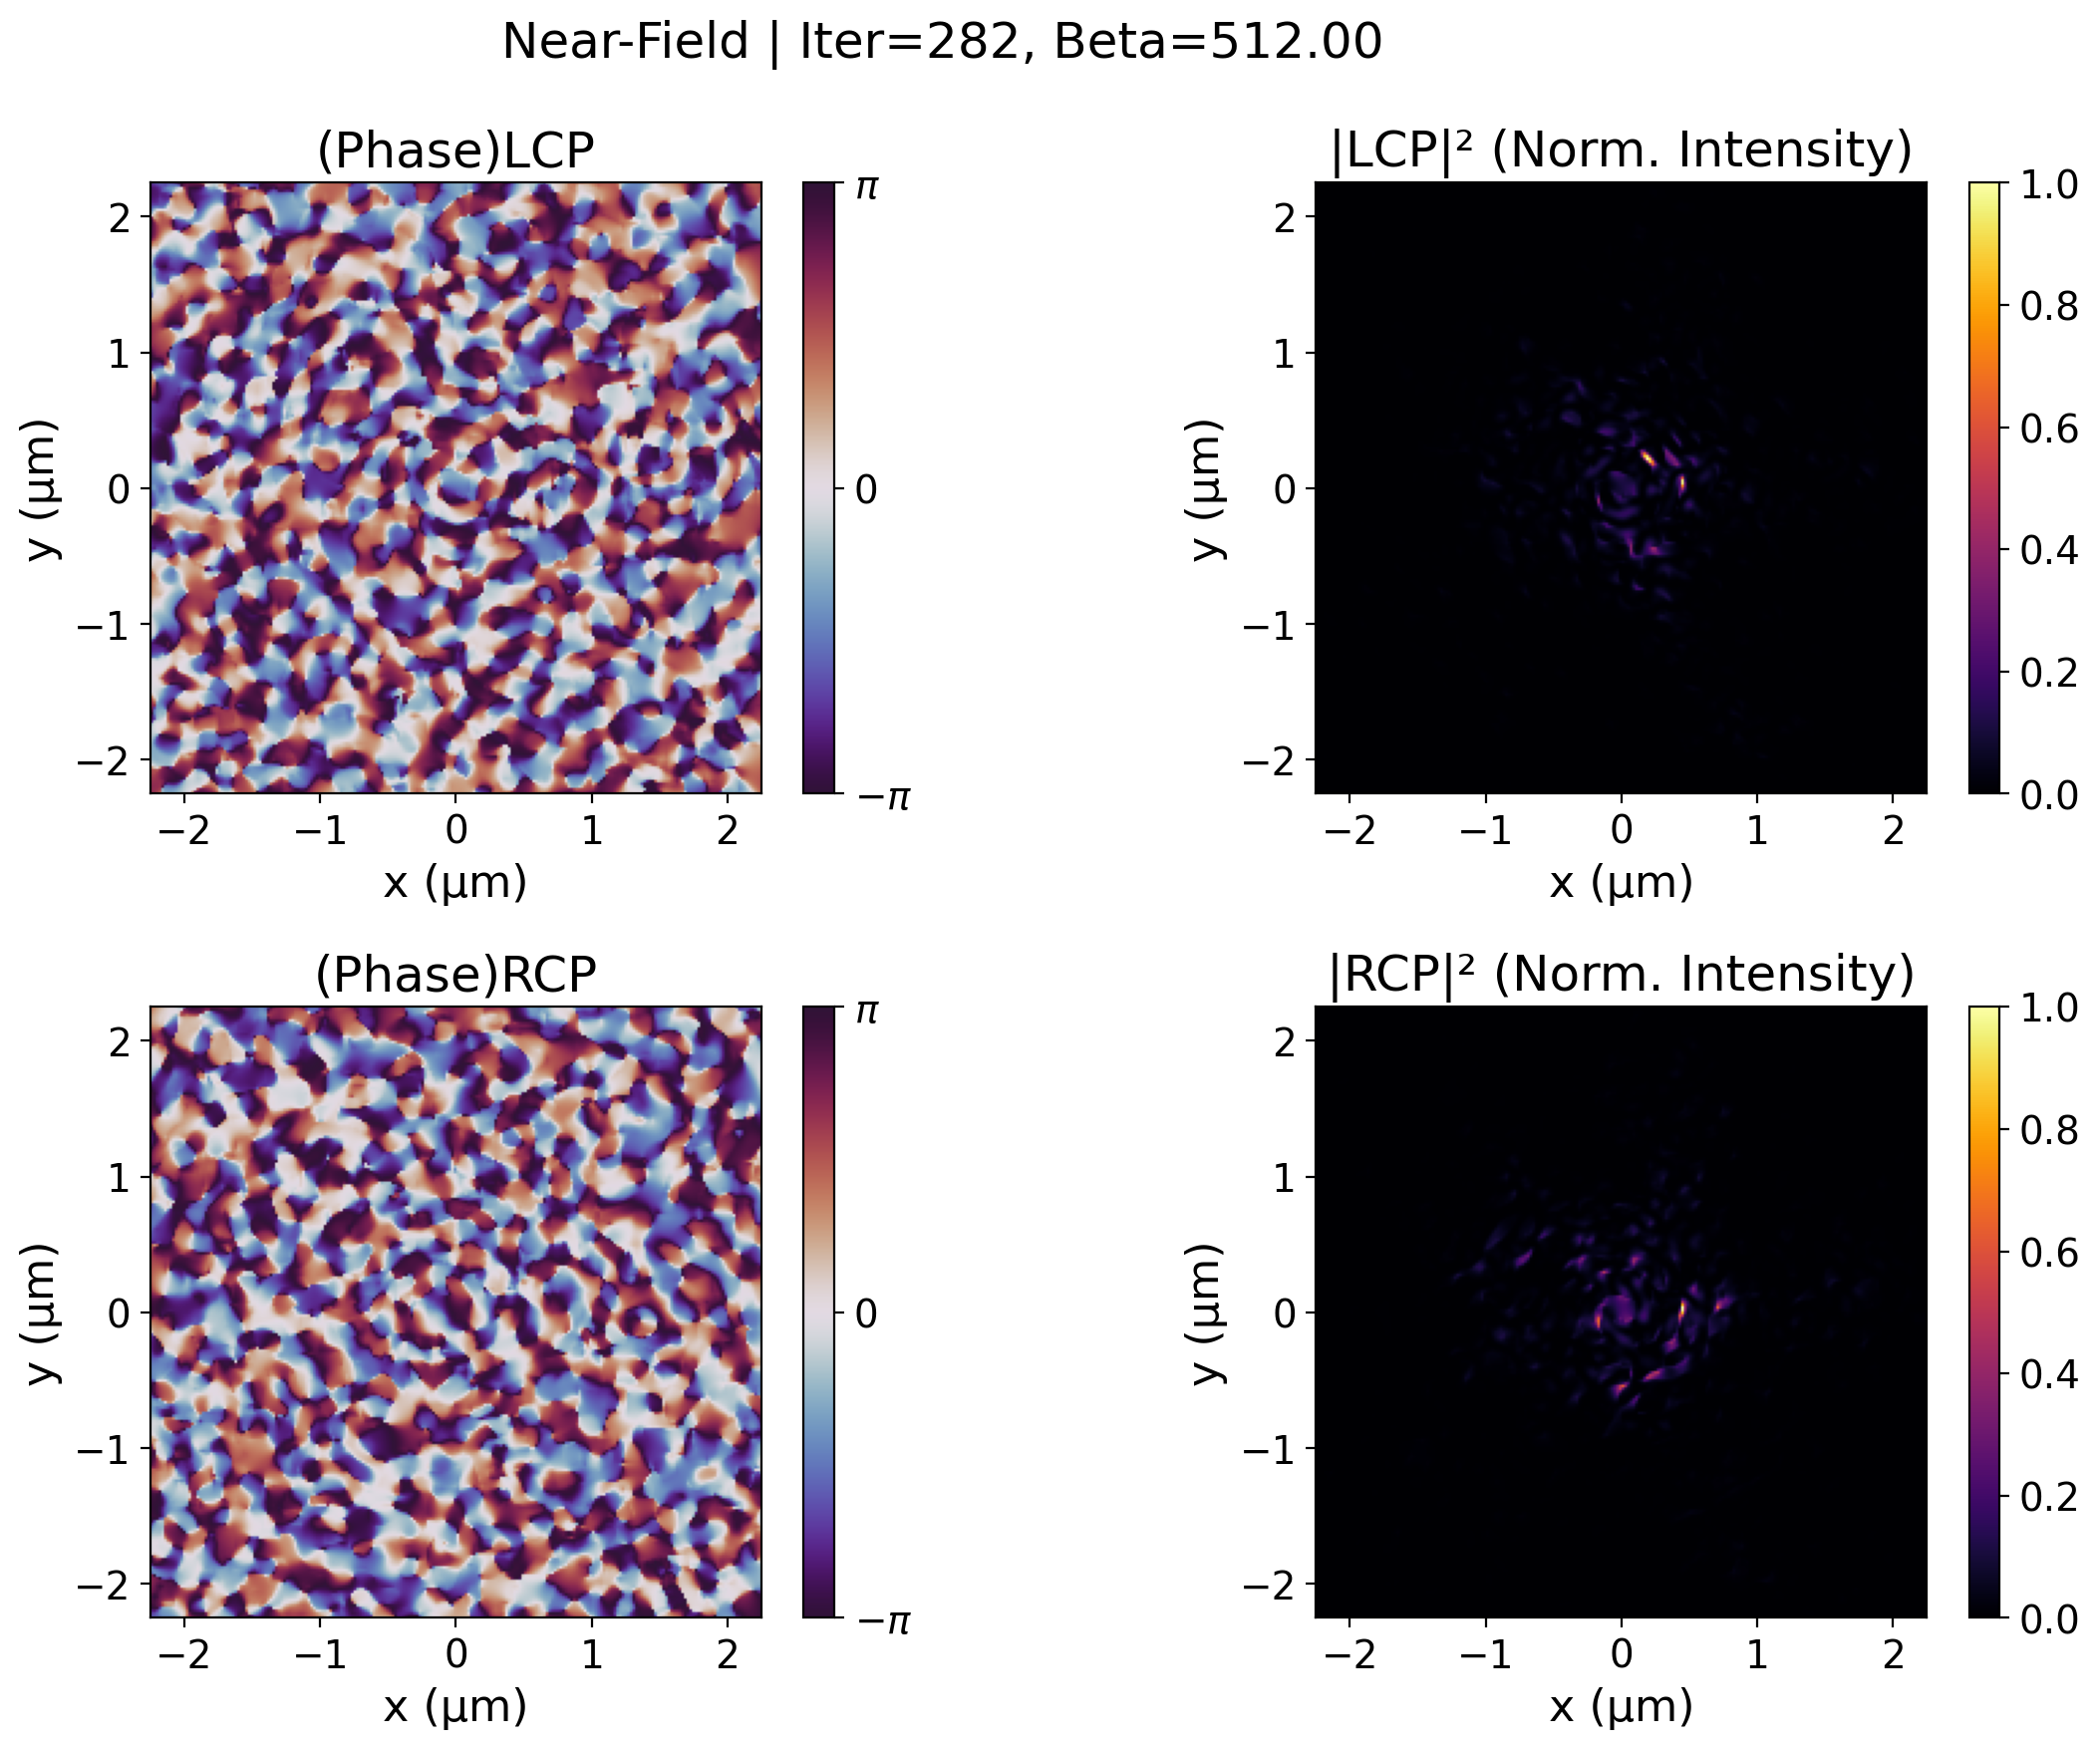
\includegraphics[width=0.31\textwidth,keepaspectratio]{img/022_phase_iter_282_beta_512.00.png} \\
    {\tiny (d) $\ell=3$} & {\tiny (e) $\ell=4$} & {\tiny (f) $\ell=5$} \\
  \end{tabular}
\end{frame}

  

\begin{frame}{Backup: Far-Field Chirality (All 6)}
  \centering
  {\footnotesize Far-field chirality at $z=10\,z_R$. Pure RCP in beam spot for all designs.}\\[4pt]
  \begin{tabular}{ccc}
    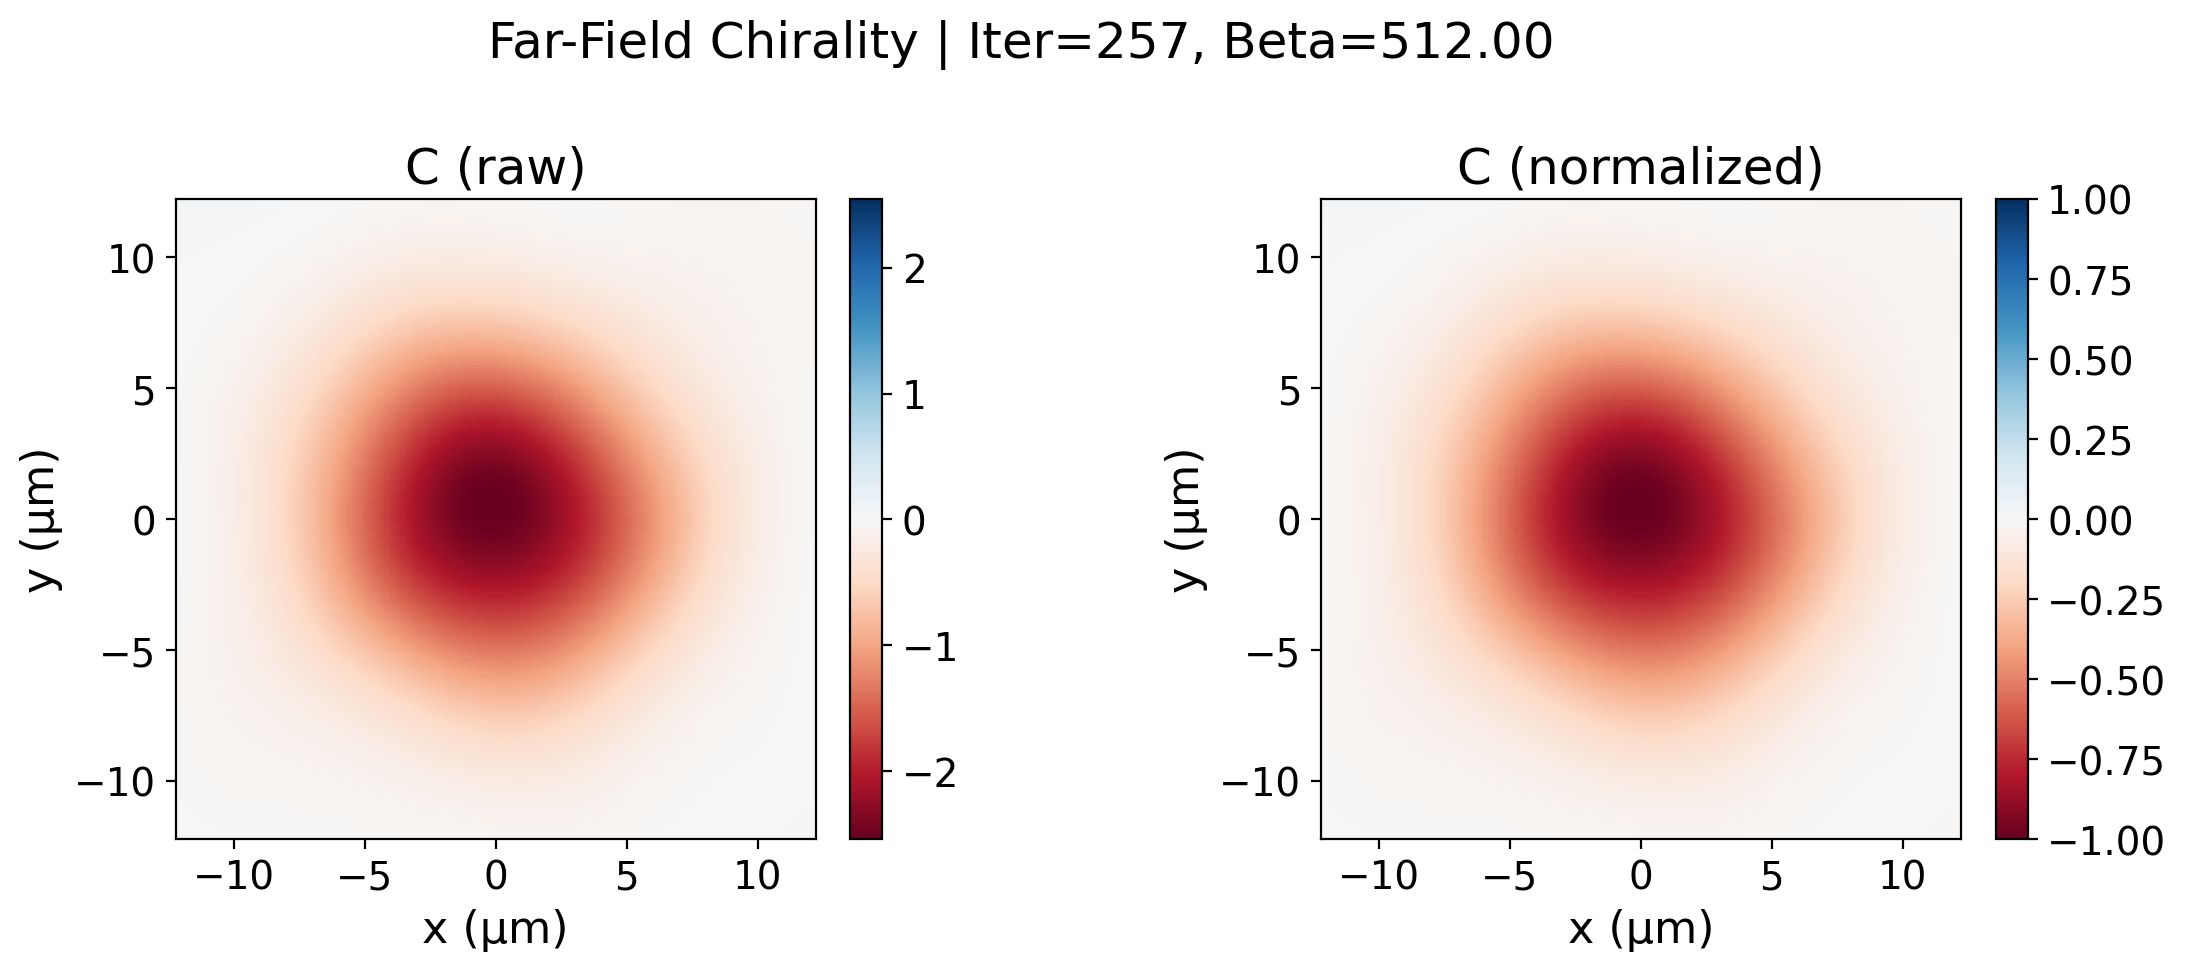
\includegraphics[width=0.31\textwidth,keepaspectratio]{img/017_ff_chirality_257_beta_512.00.png} &
    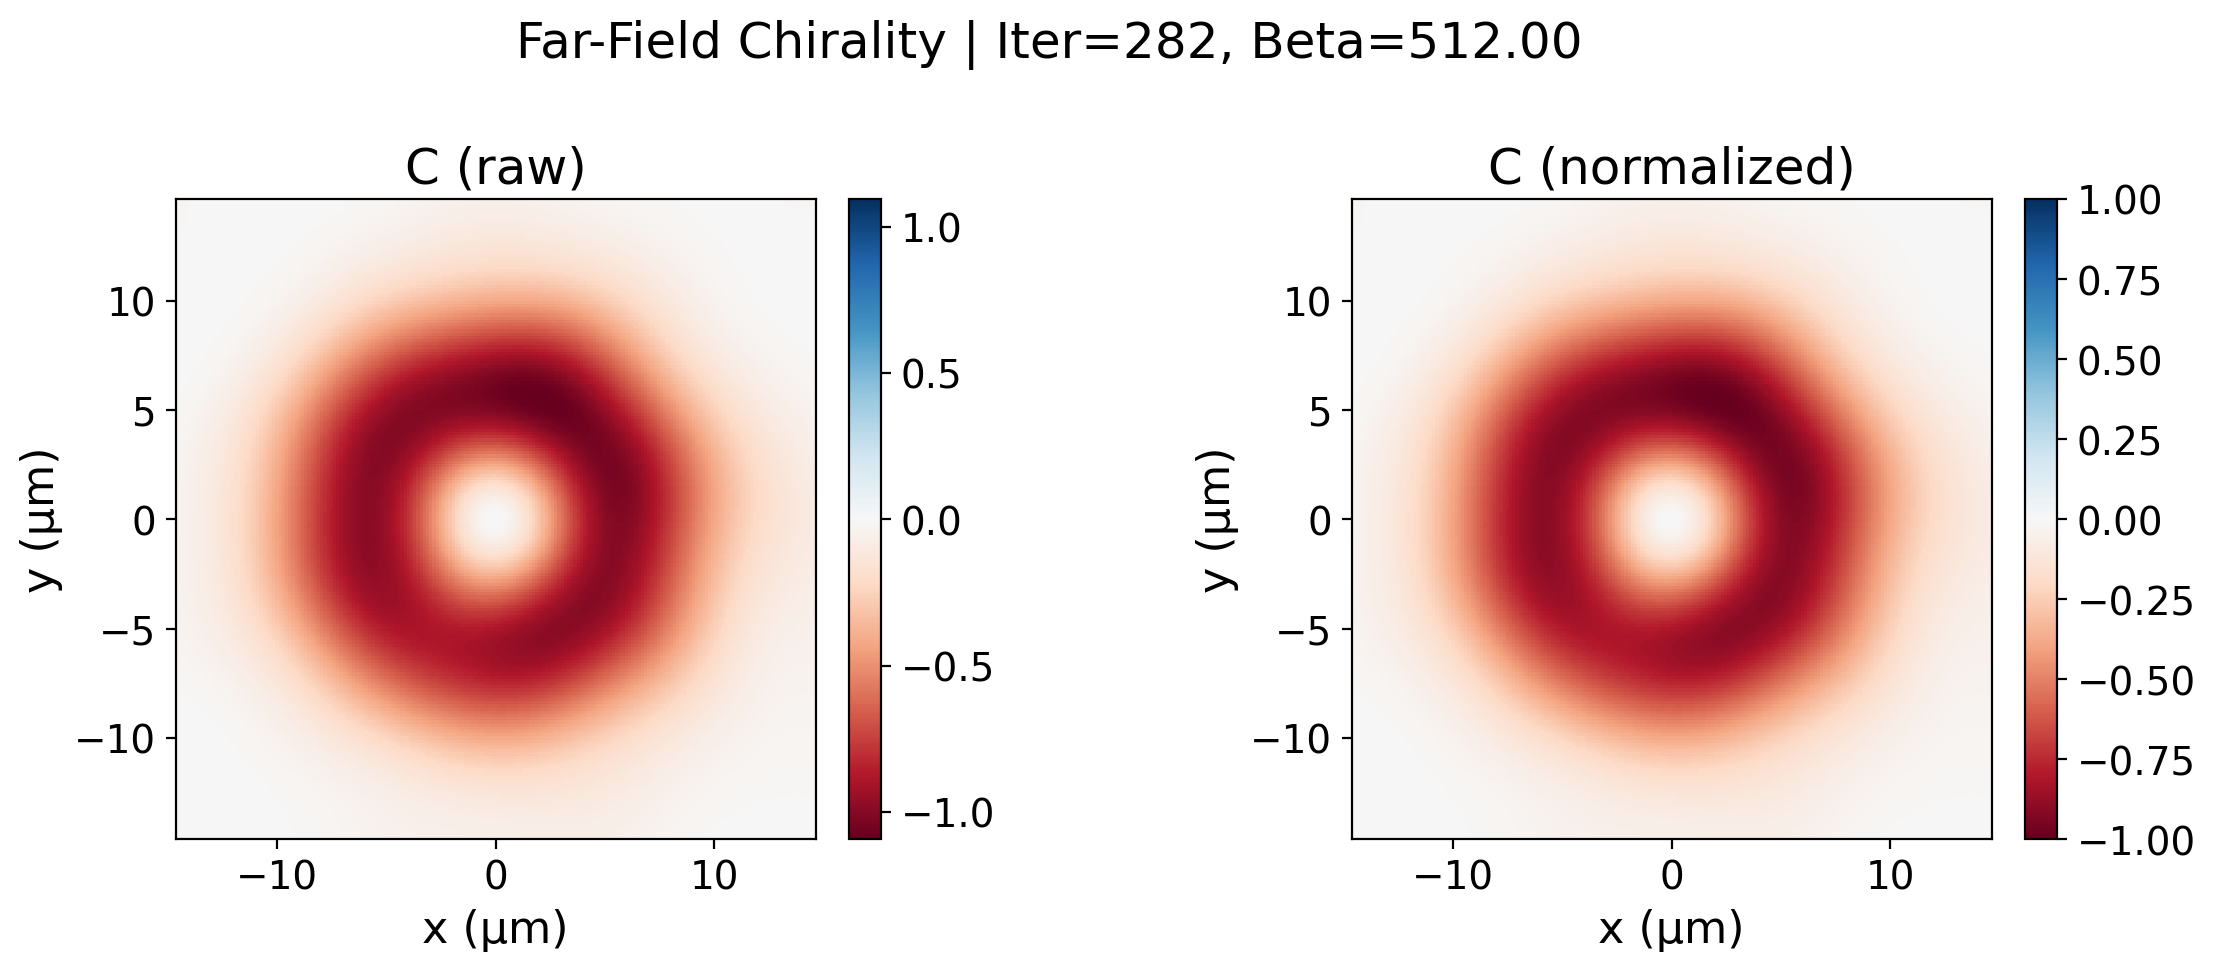
\includegraphics[width=0.31\textwidth,keepaspectratio]{img/018_ff_chirality_282_beta_512.00.png} &
    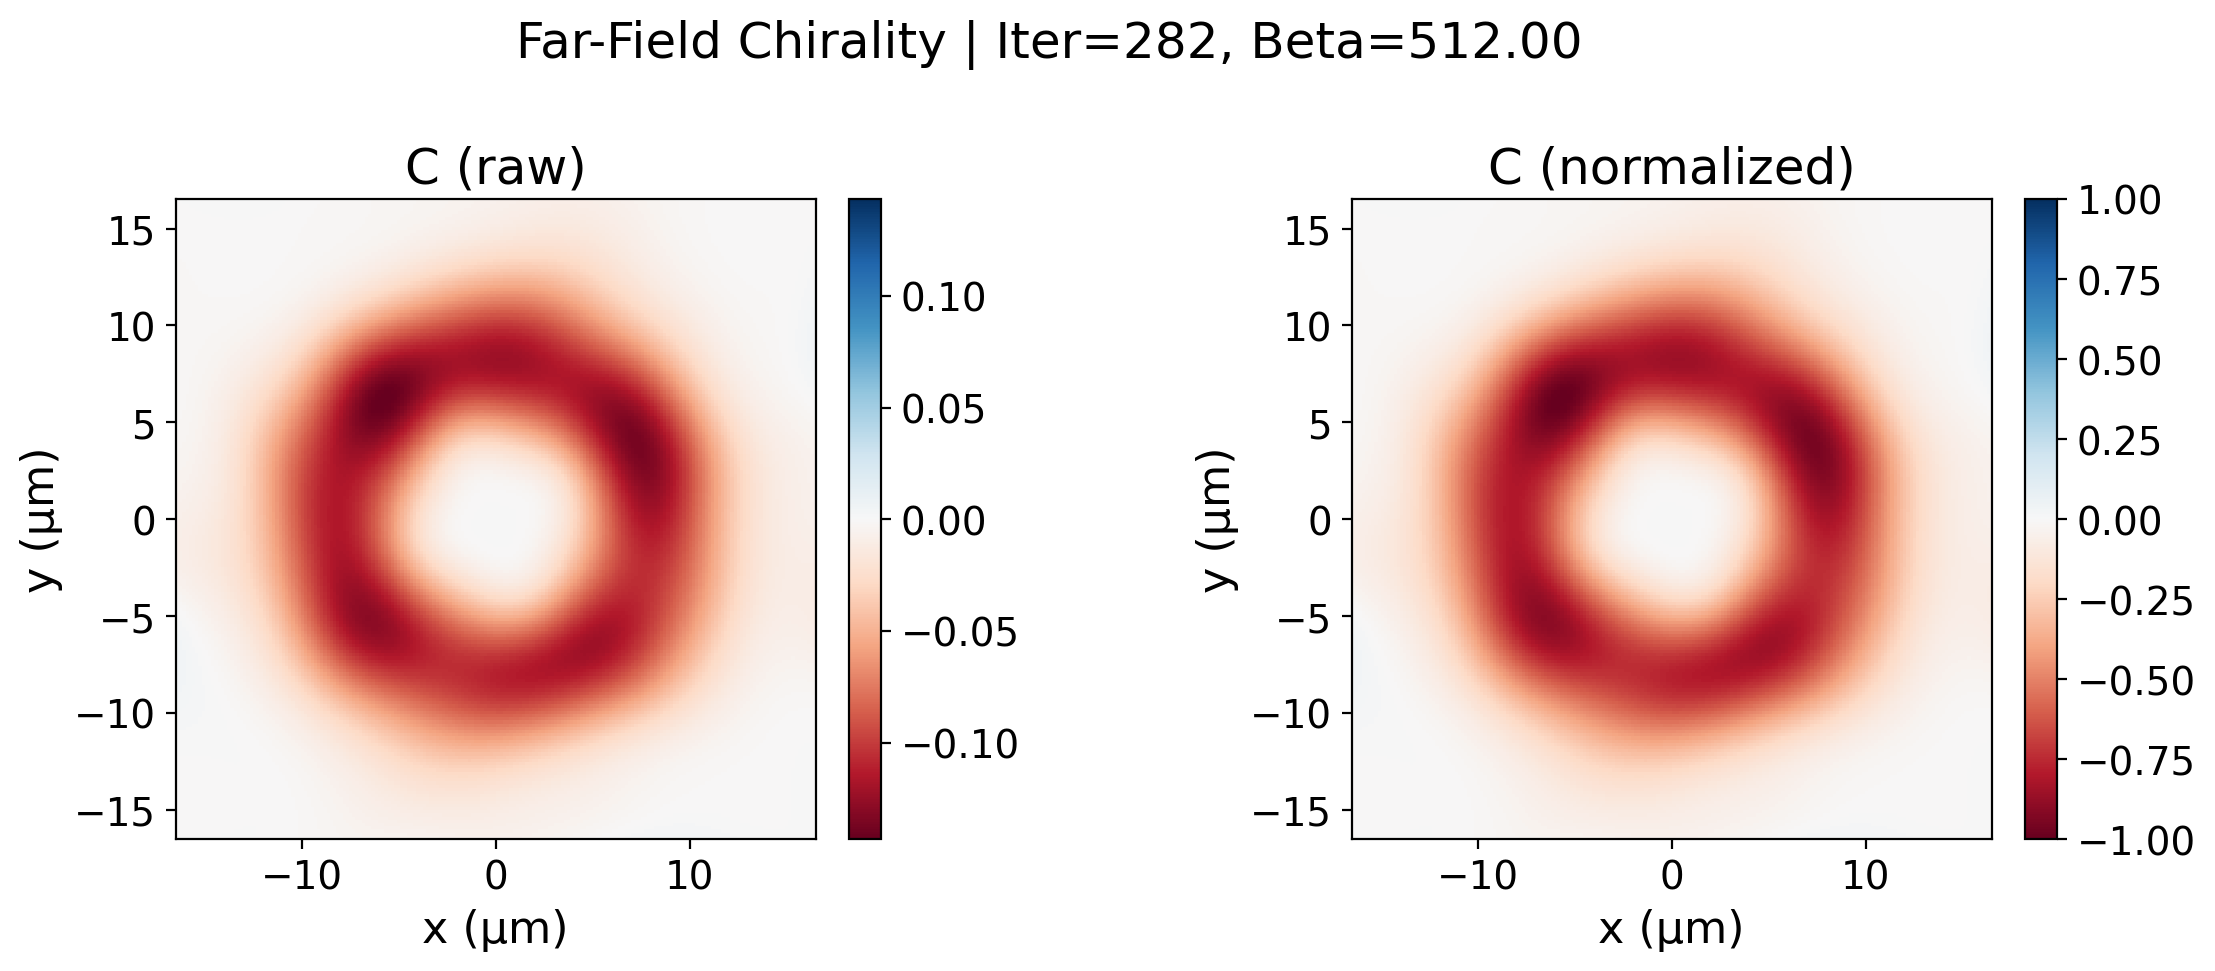
\includegraphics[width=0.31\textwidth,keepaspectratio]{img/013_ff_chirality_282_beta_512.00.png} \\
    {\tiny (a) $\ell=0$} & {\tiny (b) $\ell=1$} & {\tiny (c) $\ell=2$} \\[4pt]
    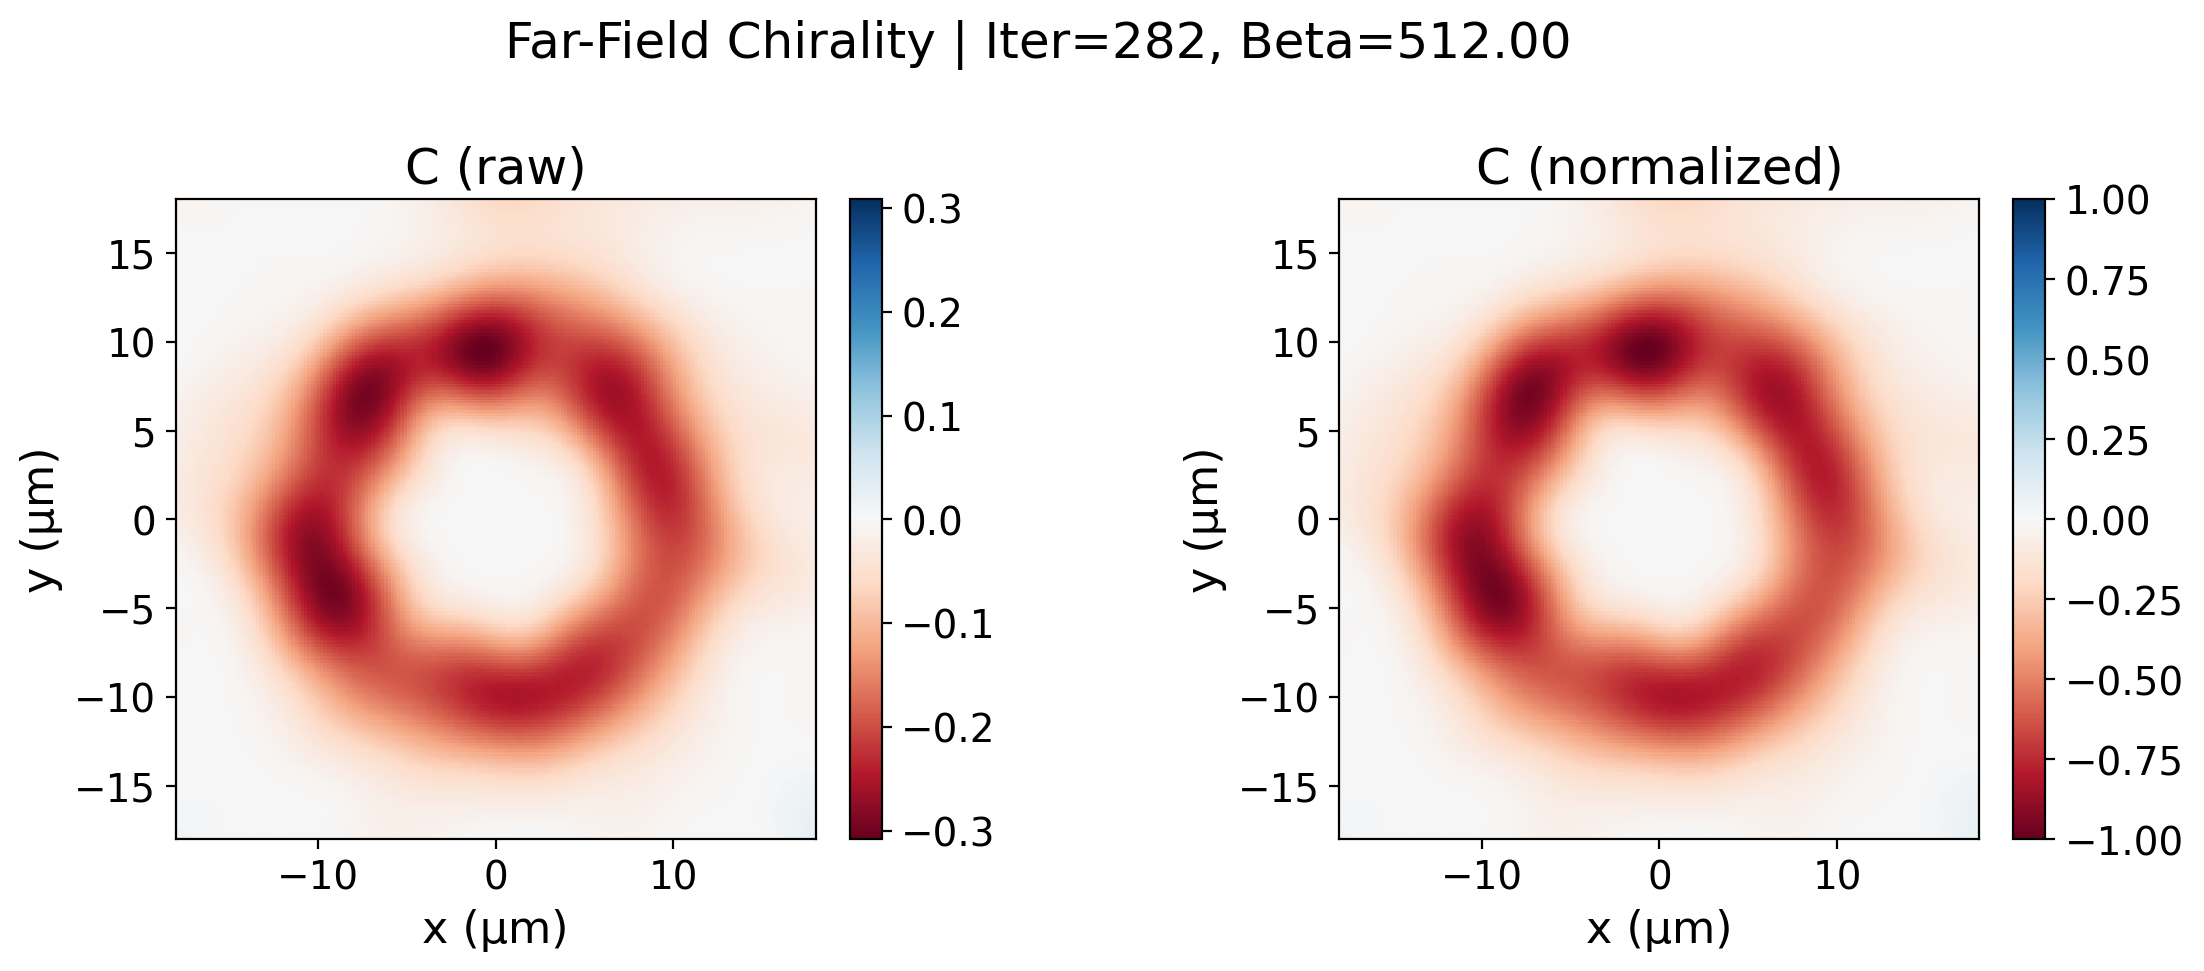
\includegraphics[width=0.31\textwidth,keepaspectratio]{img/020_ff_chirality_282_beta_512.00.png} &
    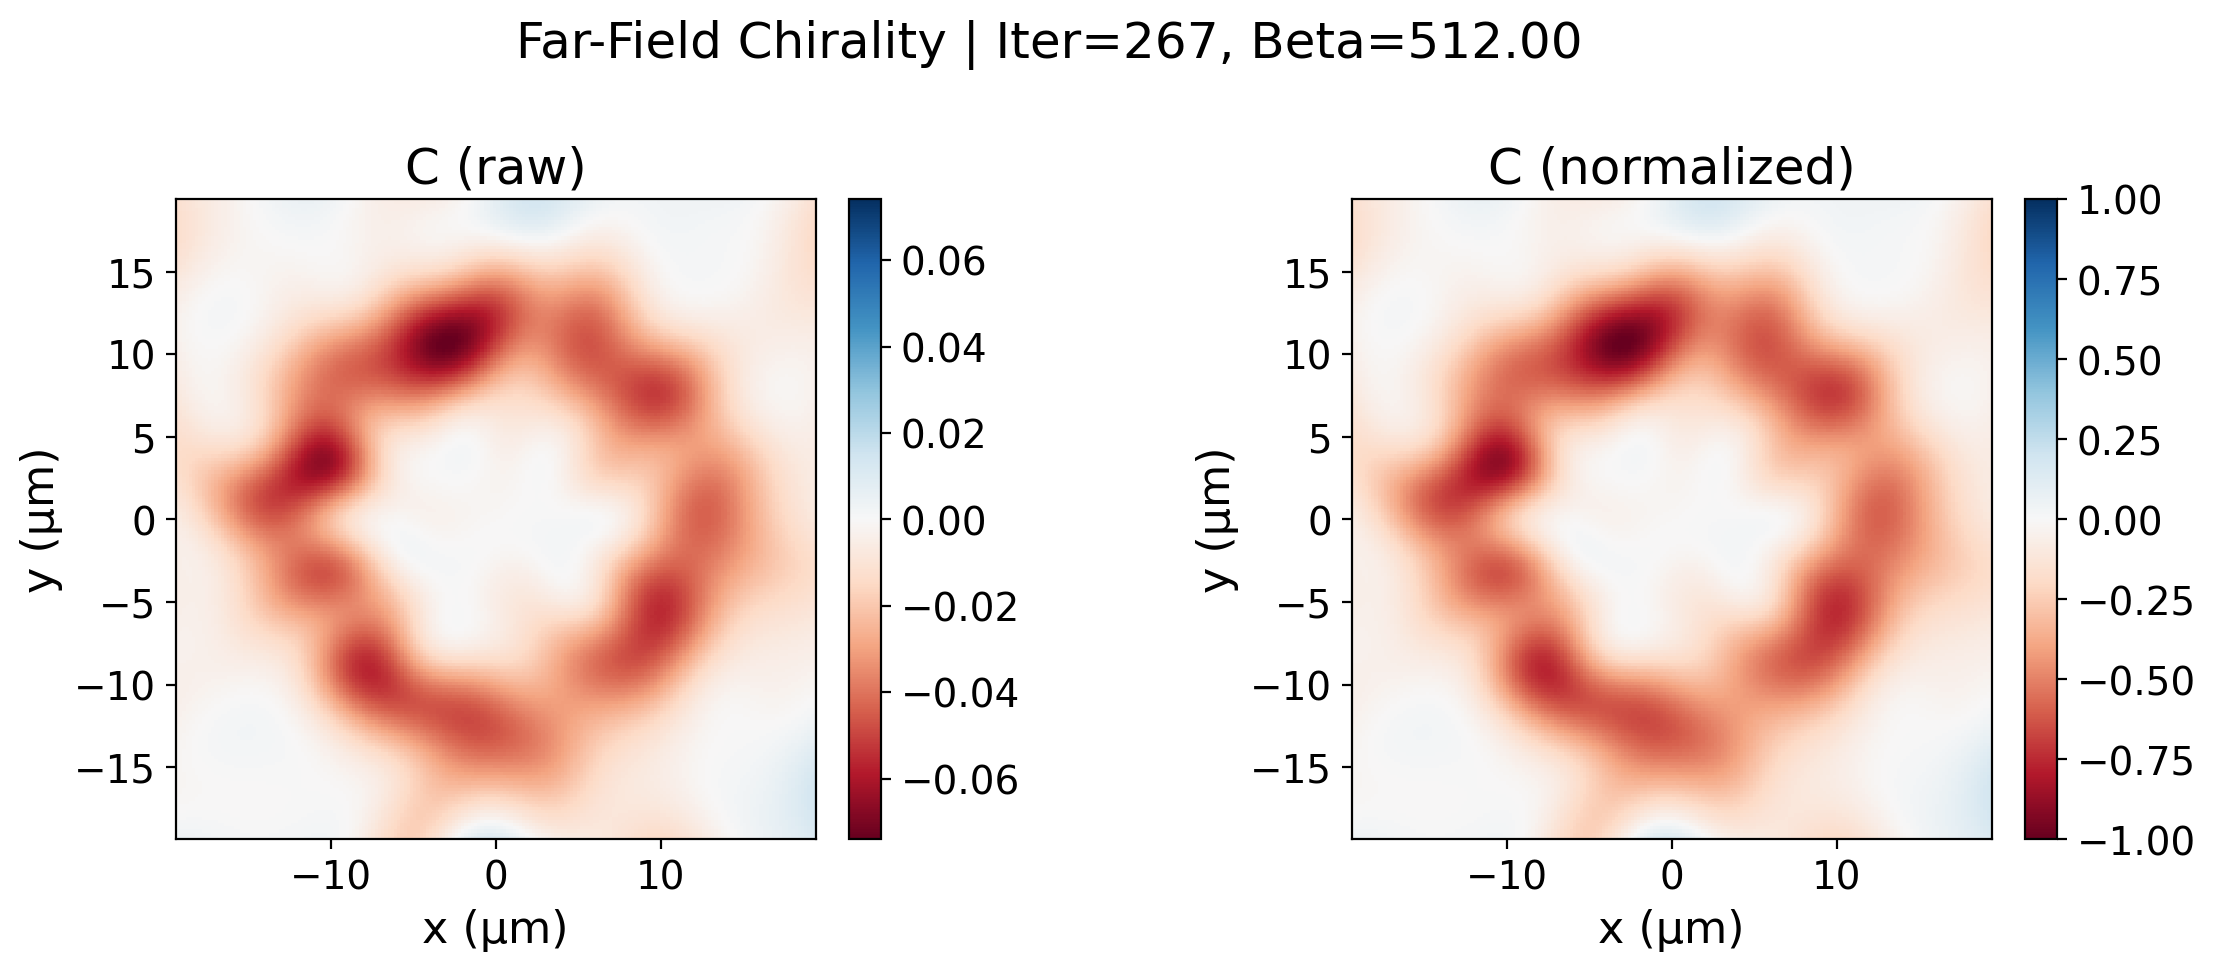
\includegraphics[width=0.31\textwidth,keepaspectratio]{img/021_ff_chirality_267_beta_512.00.png} &
    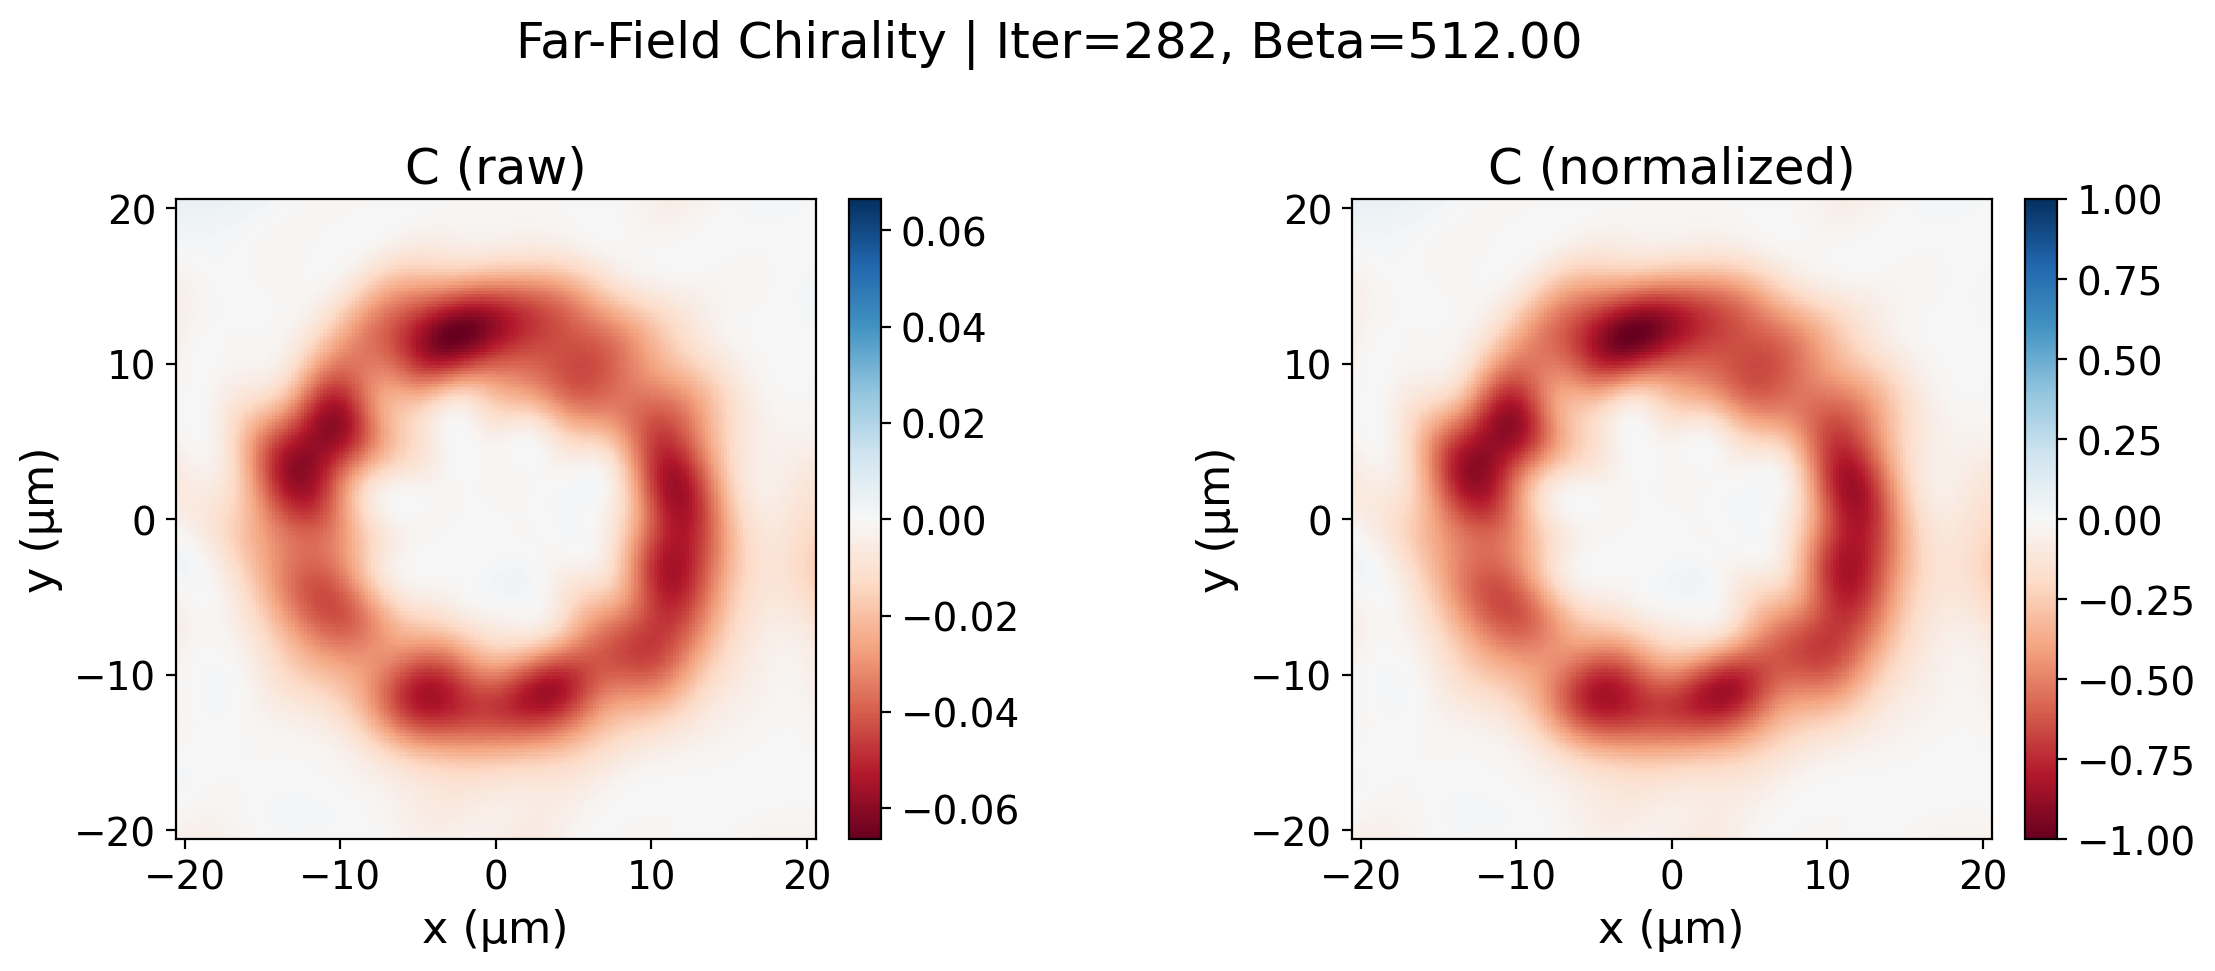
\includegraphics[width=0.31\textwidth,keepaspectratio]{img/022_ff_chirality_282_beta_512.00.png} \\
    {\tiny (d) $\ell=3$} & {\tiny (e) $\ell=4$} & {\tiny (f) $\ell=5$} \\
  \end{tabular}
\end{frame}

\begin{frame}{Backup: Compare FoMs}
  \begin{center}
    {\small $\ell=5$ , for example}\\[2pt]
    \begin{tabular}{cc}
    {\small Purity = 72.89\%, $|\text{Overlap}|^2$ = 0.89} & {\small Purity = 82.62\%, $|\text{Overlap}|^2$ = 3.96}\\
    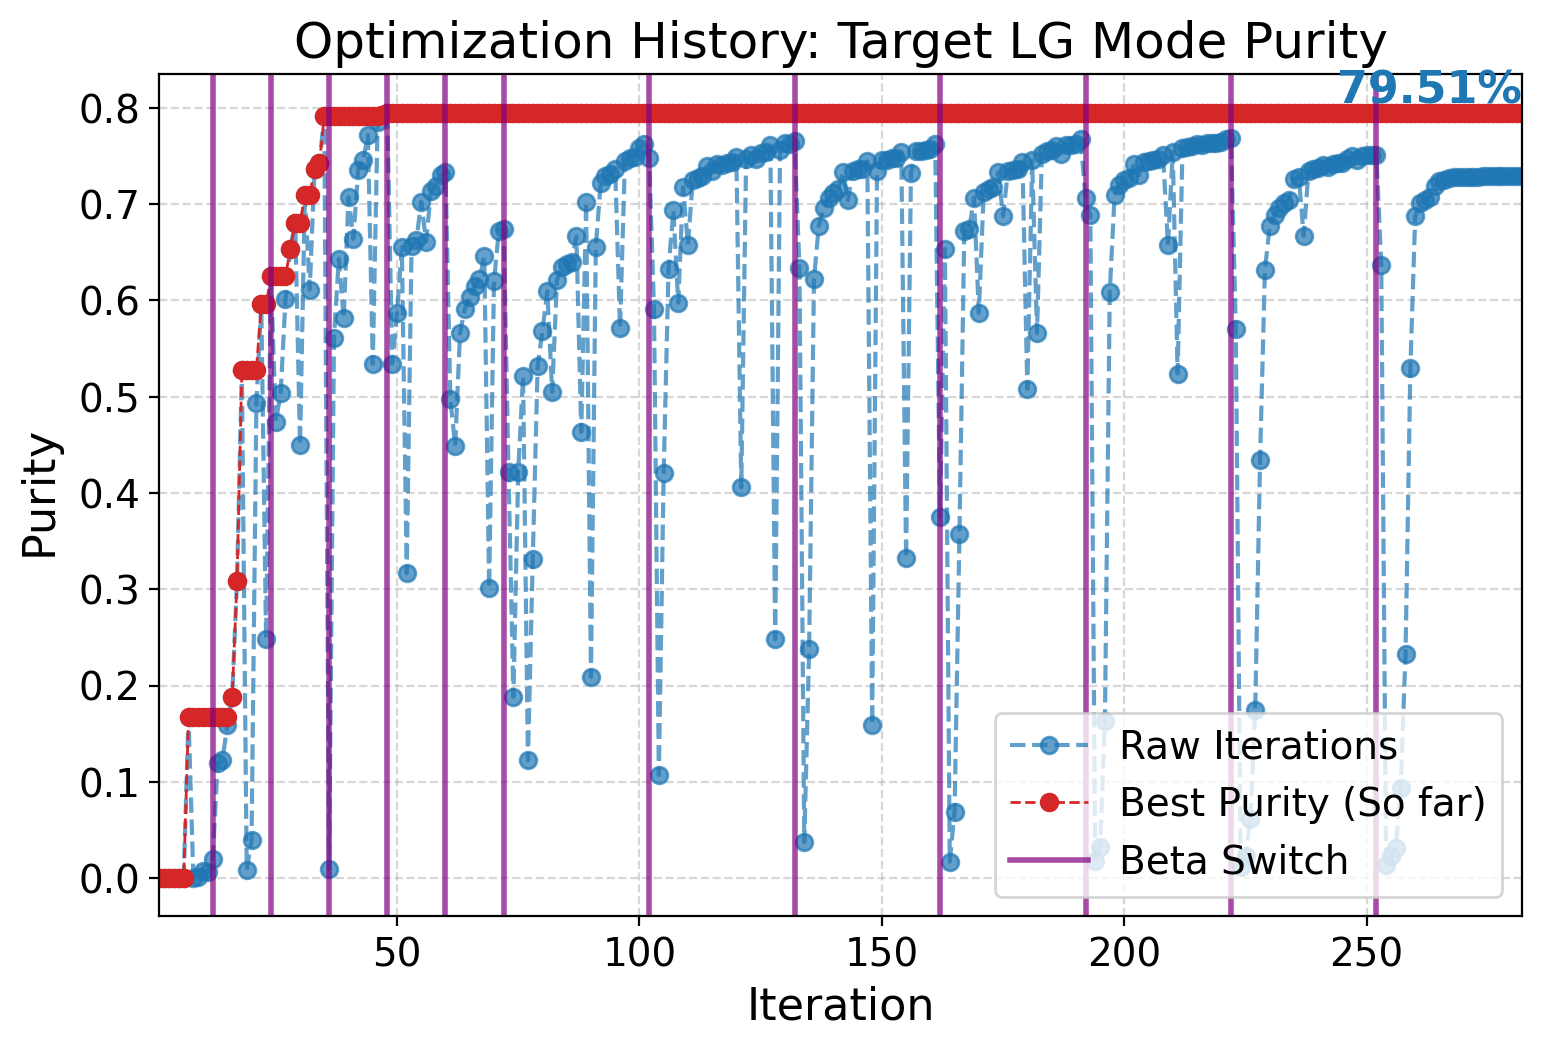
\includegraphics[width=1.0\linewidth,height=5.0cm,keepaspectratio]{img/016_purity_history_staircase.png} &
    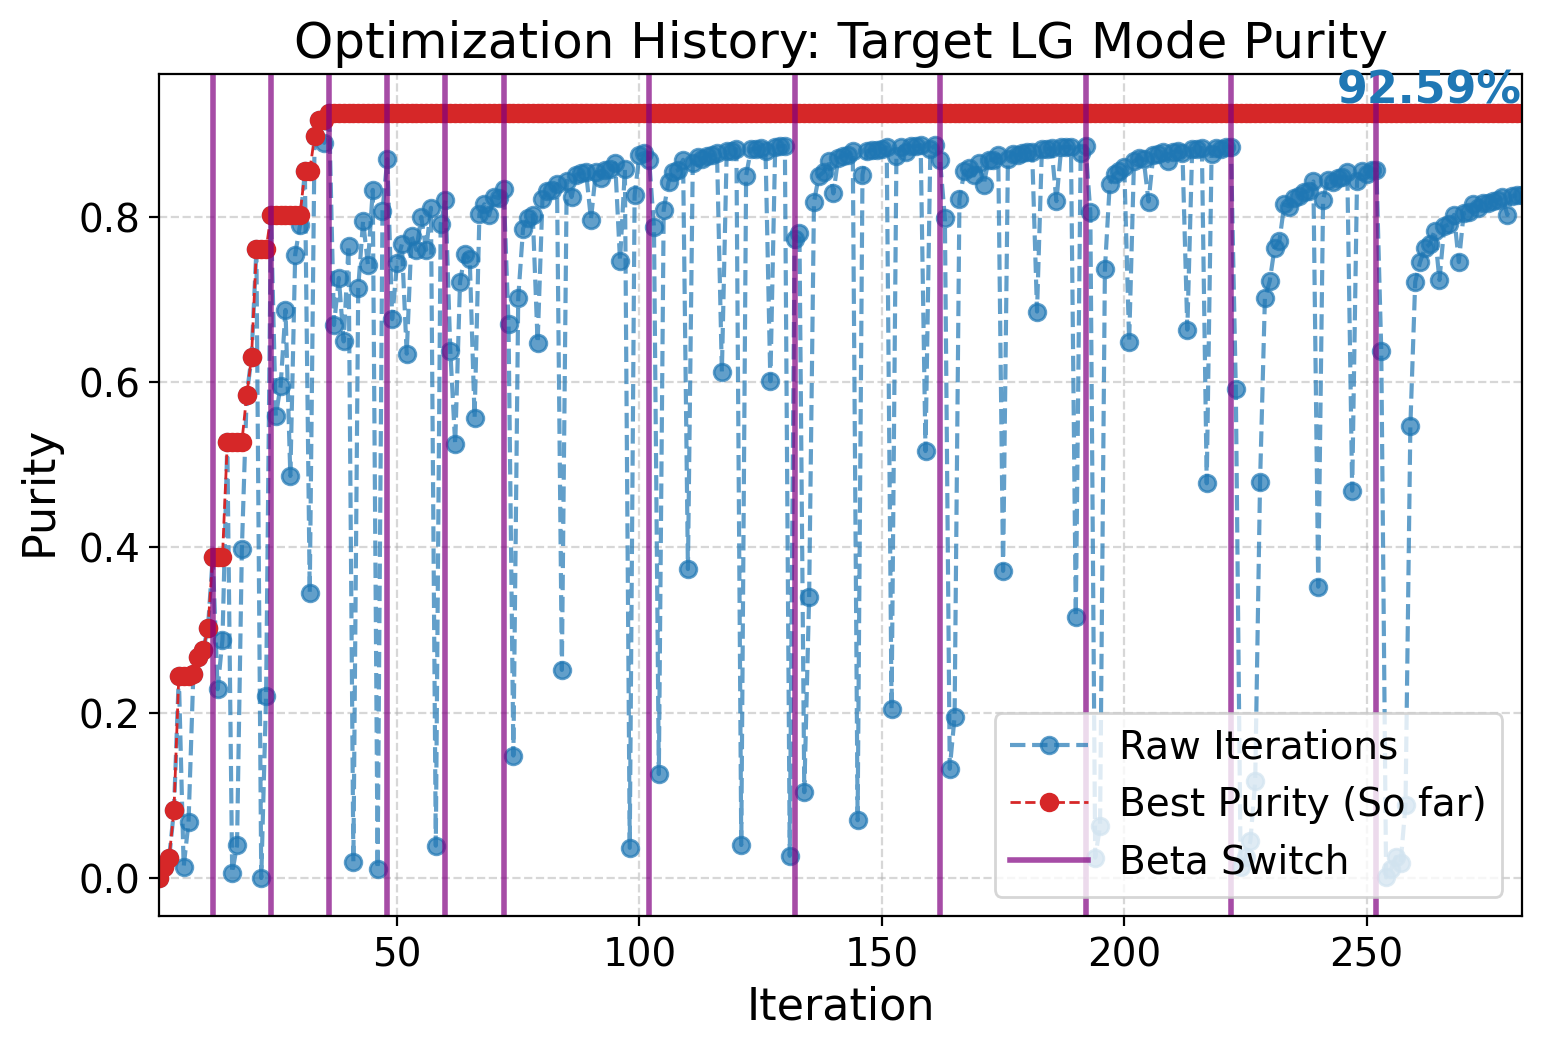
\includegraphics[width=1.0\linewidth,height=5.0cm,keepaspectratio]{img/022_purity_history_staircase.png} \\
    {\small (a) FoM I =$\dfrac{|\text{Overlap}|^{2}}{P_\text{sim} P_\text{target}}$} & {\small (b) FoM II = $\log \dfrac{|\text{Overlap}|^{2}}{P_\text{sim} P_\text{target}} +\alpha \log|\text{Overlap}|^2$}
    \end{tabular}
  \end{center}
\end{frame}

\begin{frame}[allowframebreaks]{References} 
\bibliographystyle{unsrt} 
\bibliography{ref} 
\end{frame}

\end{document}

